\documentclass[12]{ansnse}
\usepackage{authblk}
\usepackage{layouts}
\usepackage{verbatim}
\usepackage{todonotes}
\usepackage[margin=1in]{geometry}
\usepackage{lipsum}
\usepackage[tbtags]{amsmath}
\usepackage[lofdepth=2]{subfig}
\usepackage{siunitx}
\usepackage{hyperref}
\usepackage{bm}
\usepackage[nolists]{endfloat}

\hypersetup{colorlinks=true,
citecolor=black,
linkcolor=black}

% \usepackage[urw-garamond]{mathdesign}
% \usepackage[sc]{mathpazo}
% \linespread{1.05}         % Palatino needs more leading (space between lines)

\newcommand{\A}{\ensuremath{\mathcal{A}}}
\newcommand{\qp}{q^{(+)}(x)}
\newcommand{\qm}{q^{(-)}(x)}
\newcommand{\op}[1]{\ensuremath{\bm{\mathsf{#1}}}}
\newcommand{\dd}{\ensuremath{\mathop{}\!\mathrm{d}}}
\newcommand{\vP}{\ensuremath{v_{\Pi}}}
\newcommand{\Lx}{\ensuremath{\Lin_b(x)}}
\newcommand{\Lin}{\ensuremath{\mathcal{L}}}
\newcommand{\vL}{\ensuremath{v_{\Lin}}}
\newcommand{\xmid}{\ensuremath{x_{b,\mathrm{mid}}}}

\setlipsumdefault{1}

\author[1,2]{Jeremy Lloyd Conlin\footnote{\texttt{jlconlin@lanl.gov}}}
\author[2]{James Paul Holloway}
\affil[1]{\normalsize\emph{Los Alamos National Laboratory\authorcr}
\emph{PO Box 1663, MS F663, Los Alamos, NM 87545}}
\affil[2]{\normalsize\emph{University of Michigan, College of Engineering\authorcr}
\emph{Department of Nuclear Engineering and Radiological Sciences\authorcr}
\emph{1221 Beal Avenue, Ann Arbor, MI  48109-2106}}

\title{\sffamily\bfseries\Large Monte Carlo Application of Arnoldi's Method for Acceleration of Eigenvalue and Fission Source Convergence}

\date{}

\begin{document}
\maketitle
\ansabstract{This paper introduces the explicitly restarted Arnoldi's method for calculating eigenvalues and eigenvectors in a Monte Carlo criticality calculation.  Arnoldi's method is described along with the power method.  The power method has been used for decades for Monte Carlo criticality calculations despite the availability of other algorithms with better convergence properties.  The Monte Carlo application of the transport-fission operator of the Boltzmann transport equation is defined and the Monte Carlo implementation of both Arnoldi's method and the power method are described.  A brief discussion of eigenvalue and fission source convergence is given.  Numerical simulations of 1-D slab geometries are presented, demonstrating the convergence of both the eigenvalue and fission source (as measured by the Shannon entropy) for both Arnoldi's method and the power method.  The results show that Arnoldi's method does not need to discard iterations like the power method because both the eigenvalue and fission source appear to converge immediately, even for problems with high dominance ratios.
}

\begin{doublespace}
%\begin{multicols}{2}
\begin{comment}
 \pagediagram
\currentpage
\pagedesign

The textwidth is \printinunitsof{pt}\prntlen{\textwidth} which is also \printinunitsof{in}\prntlen{\textwidth} or \printinunitsof{mm}\prntlen{\textwidth}. 

The textheight is \printinunitsof{pt}\prntlen{\textheight} which is also \printinunitsof{in}\prntlen{\textheight} or \printinunitsof{mm}\prntlen{\textheight}. 
\end{comment}

\section{Introduction}
For decades\cite{Goad:1959A-Mon-0,Kaplan:1958Monte-0,Lieberoth:1968A-Mon-0,Mendelson:1968Monte-0} the power method has been the algorithm of choice for estimating the fundamental eigenvalue and eigenvector of the transport-fission operator of the Boltzmann transport equation in Monte Carlo criticality calculations.  The power method is a robust application of a Krylov subspace method.  A Krylov subspace method is one where only the knowledge of the application of a linear operator to a vector is required to estimate the eigenvalues and eigenvectors of the linear operator; an explicit (e.g. matrix) form of the linear operator is not necessary.  The Monte Carlo implementation of the power method for neutral particle transport applications is straightforward making it desirable for criticality applications.

Despite the robust and uncomplicated features of the power method, it suffers from slow convergence to the desired eigenvalue and fission source.  The convergence rate is proportional the dominance ratio, the ratio of the first higher-order eigenvalue to the fundamental eigenvalue, \[DR = \lambda_1/\lambda_0.\]  For many particle transport calculations of interest, this ratio is close to unity causing slow convergence.

Much work\cite{Brown:2009A-Rev-0} has been done during the last decade investigating the convergence of the both the eigenvalue and fission source in Monte Carlo criticality applications.  \citet{Ueki:2003Infor-0,Ueki:2005Stati-0} have shown the necessity of performing many discarded power iterations before the results from the power method iterations can be used for estimating the fundamental eigenvalue without biasing the results with bad eigenvalue estimates or a poorly converged fission source.

Arnoldi's method\cite{Arnoldi:1951The-P-0} is another Krylov subspace method commonly used to estimate eigenvalues and eigenvectors of linear operators for which an explicit form of the operator is not known or is expensive to calculate and/or store.  \citet{Warsa:2004Krylo-0} have shown Arnoldi's method to provide a significant improvement over the power method in deterministic calculations, achieving cost savings of 1--2 orders of magnitude using Arnoldi's method over the power method.  For Monte Carlo criticality calculations, we have demonstrated\cite{Conlin:2008Arnol-0} the capability of Arnoldi's method in calculating multiple eigenvalues and eigenvectors for 1-D geometries.  

In this paper we will describe Arnoldi's method can be used to accelerate the convergence of the eigenvalue and the fission source as compared to the power method in a Monte Carlo criticality application.  In Section \ref{sec:KrylovMethods}, we review the power method (Section \ref{sec:PowerMethod}) and introduce Arnoldi's method and our one-dimensional implementation will be described (Section \ref{sec:ArnoldiExplanation}).  In Section \ref{sec:Convergence}, we briefly review how fission source convergence is quantified and describe how it is done with Arnoldi's method.  In Section \ref{sec:Numerical}, we will compare Arnoldi's method to the power method for a few problems with high dominance ratios.  In Section \ref{sec:Conclusions} we conclude and propose future research for Arnoldi's method.  %These problems were chosen because their eigenvalues have been published and the difficulties in converging to the correct eigenvalue and fission source have been investigated; we will be able to compare our results to those previously published.

\section{Monte Carlo Eigenvalue Calculations with Krylov Subspace Methods}\label{sec:KrylovMethods}
Krylov subspace methods\cite{Saad:1992Numer-0} approximate solutions (i.e. eigenvalues and eigenvectors) from a subspace of the form
\begin{equation}
    \mathcal{K}_m~=~\mathrm{span}\left\{v, \op{A} v, \op{A}^2v, \ldots , \op{A}^{m-1}v\right\},
    \label{eq:Krylov}
\end{equation}
where $v$ is some function or vector and $\op{A}$ is a linear operator.  The basis vectors of the Krylov subspace,
\begin{equation}
    \mathcal{K}_m~=~\mathrm{span}\left\{v_1, v_2, \ldots, v_{m}\right\},
    \label{eq:KrylovBasisVectors}
\end{equation}
are the results of applying the linear operator to $v$ multiple times, $v_i = \op{A}^{i-1}$.  Note that to calculate the $n$-th basis vector, one doesn't need to apply \op{A} \mbox{$(n-1)$} times; it is sufficient to apply \op{A} to the previously calculated basis vector.  Knowing this, we can see that Krylov subspace is calculated iteratively with one basis vector calculated at each iteration.

Krylov subspace methods do not require an explicit form of the operator $\op{A}$, but do rely on the existence of a procedure or algorithm to apply the linear operator, $\op{A}$, to a vector, $v$.

The iterative process of creating a Krylov subspace by the application of the linear operator on a vector makes Krylov subspace techniques attractive to Monte Carlo particle transport calculations.  To define the linear operator for Monte Carlo criticality applications we begin with the Boltzmann transport eigenvalue equation
\begin{multline}
    \mathbf{\Omega}\cdot\mathbf{\nabla}\psi(\mathbf{r},\mathbf{\Omega})+\Sigma_t\psi(\mathbf{r},\mathbf{\Omega}) = \\
    \frac{\Sigma_s}{4\pi}\int \psi(\mathbf{r},\mathbf{\Omega})\;d\Omega + \frac{1}{k}\frac{\nu\Sigma_f}{4\pi}\int \psi(\mathbf{r},\mathbf{\Omega})\;d\Omega,
\end{multline}
and write it in operator form
\begin{subequations}\begin{align}
    (\op{L} + \op{C} - \op{S})\psi &= \frac{1}{k}\op{F}\psi \\
    \op{T}\psi &= \frac{1}{k}\op{F}\psi \label{eq:Opr}
\end{align}\end{subequations}
where $\op{L}, \op{C},$ and $\op{S}$ are the leakage, collision, and scattering operators respectively and $\op{F}$ is the fission operator.  The operator $\op{T}$ is the transport-collision operator.  The left-hand side represents the neutron loss and scattering mechanisms and the right-hand side represents the neutron gain mechanism.  We define
\begin{equation}
    v \equiv \op{F}\psi
\end{equation}
as the Monte Carlo fission source and
\begin{equation}
    \A \equiv \op{F}\,\op{T}^{-1}
\end{equation}
as the transport-fission operator.  We can manipulate \eqref{eq:Opr} to obtain
\begin{equation}
    \A v = kv. \label{eq:evalue}
\end{equation}
This is a standard eigenvalue problem with $k$ and $v$ the eigenvalue and eigenvector of the transport-fission operator, \A.  The operation of \A{} on any fission source can be evaluated by Monte Carlo, as described next.
\subsection{Monte Carlo Application of Transport- Fission Operator on Fission Source}\label{sec:AApplication}
A fission source, $v$, is a distribution of fission neutrons, or---in the case of the first iteration---a predefined list of locations where fission neutrons may be found.  The Monte Carlo application of \A{} to $v$ is done by randomly picking fission neutrons from the fission source, transporting them through the medium and storing any new neutrons created by fission.  These new fission neutrons make up a new fission source and are the result of the operation of \A{} on $v$.  It is important to note that any of the standard variance reduction techniques can be used to reduce the statistical uncertainty of the application of \A.  

This application of the transport-fission operator will be used in both the power method and Arnoldi's method.  The only difference between the two applications is the way that fission neutrons are sampled from the fission source; in the power method, fission neutrons are sampled from discrete fission sites while in Arnoldi's method, fission neutrons are sampled from a discretized fission source.  The specifics of each method are described in the following two sections.

\subsection{Power Method}\label{sec:PowerMethod}
The power method is a straightforward implementation of a Krylov subspace method.  It begins with an estimate of the fundamental eigenvalue, $k$, and eigenvector $v$.  At each iteration the linear operator, \A, is applied to a fission source, which is then normalized by the estimate of the eigenvalue,
\begin{equation}
    v_{j+1} = \frac{1}{k_j}\A v_j.
    \label{eq:PowerMethodVector}
\end{equation}
Here $v_{j}$ is the estimate of the fundamental eigenvector calculated in the \mbox{$j$-th} iteration of the power method.  The fundamental eigenvalue is estimated in the \mbox{$\left(j+1\right)$-th} iteration as
\begin{equation}
    k_{j+1} = k_j\frac{\int \A v_j}{\int v_j} = k_j \frac{\int v_{j+1}}{\int v_j}.
    \label{eq:PowerMethodValue}
\end{equation}
Using Eqs. \eqref{eq:PowerMethodVector}--\eqref{eq:PowerMethodValue} and knowing how to apply the transport-fission operator as discussed in the previous section, we can use the power method to estimate the fundamental eigenvalue and eigenvector of the transport-fission operator, \A.  Note that the power method only stores the previous fission source and so discards information about the previously calculated basis vectors of the Krylov subspace.

The eigenvalue estimates calculated at the end of each power iteration are stored.  The mean, $\overline{k}$, and variance, $\sigma^2$, of these eigenvalue estimates can be estimated as
\begin{align}
    \overline{k} &= \frac{1}{N}\sum_{j=1}^N k_j \label{eq:meanEigenvalue} \\
    \sigma^2 &= \frac{1}{N}\frac{1}{N-1} \sum_{j=1}^N \left(k_j - \overline{k}\right)^2, \label{eq:varEigenvalue}
\end{align}
where $N$ is the number of eigenvalue estimates.  The standard deviation, $\sigma$, of the mean of the eigenvalue estimates is a measure of the statistical uncertainty in the mean eigenvalue estimate.

\begin{comment}
The figure of merit (FOM) is a measure of the efficiency of the calculation.  The FOM is calculated as
\begin{equation}
    \mathrm{FOM} = \frac{1}{\sigma^2 T}.
    \label{eq:FOM}
\end{equation}
where $T$ is the computational time spent and $\sigma^2$ is the variance.
\end{comment}

To examine the convergence rate of the power method we note that in Eq. \eqref{eq:PowerMethodVector}, $v_{j} = \A^{j}v$.  We can write $v_j$ as a linear combination of the eigenvectors of \A
\begin{align}
    v_{j+1} &= c_0\A^{j+1}x_0 + \cdots + c_{n-1}\A^{j+1}x_{n-1} \\
    \A v_{j} &= c_0\lambda_0^{j+1}x_0 + \cdots + c_{n-1}\lambda_{n-1}^{j+1}x_{n-1}
    \label{eq:LinearCombination}
\end{align}
where $\lambda_0, \ldots, \lambda_{n-1}$ and $x_0, \ldots, x_{n-1}$ are the \mbox{$n-1$} eigenvalues and eigenvectors of \A{} with $\left(\lambda_0, x_0\right)$ being the fundamental eigenpair; $c_0, \ldots, c_{n-1}$ are just some constants.

With a little bit of algebra we can rewrite Eq. \eqref{eq:LinearCombination} as
\begin{equation}
    \A v_j = c_0x_0 + \mathcal{O}(\lambda_1/\lambda_0)^j.
    \label{eq:PowerMethodOrderDemonstration}
\end{equation}
Eq. \eqref{eq:PowerMethodOrderDemonstration} is equivalent to Eq. \eqref{eq:PowerMethodVector} and shows that the power method converges no faster than the dominance ratio $\lambda_1/\lambda_0$.

\subsection{Arnoldi's Method}\label{sec:ArnoldiExplanation}
Arnoldi's method\cite{Arnoldi:1951The-P-0} iteratively builds a Krylov subspace by applying the linear operator to a vector in the same manner as in the power method.  However, Arnoldi's method retains, orthogonalizes, and normalizes the basis vectors at each iteration.  Arnoldi's method stores all the computed basis vectors, and uses the information so retained to improve the convergence compared to the power method.  The orthonormalized basis vectors are called Arnoldi vectors.

Arnoldi's method begins like the power method with a vector which is then normalized
\begin{equation}
    v_1 = \frac{v}{\|v\|_2},
\end{equation}
where
\begin{equation}
    \|v\|_2 = \langle v, v\rangle^{1/2}
\end{equation}
is just the Euclidean norm of the vector $v$.  $v_1$ is the first basis vector of the Krylov subspace.

At the $m$-th iteration of Arnoldi's method the linear operator is applied to a vector, $v_m$, giving $\A v_m$.  This result is then orthogonalized against all previously calculated Arnoldi vectors
\begin{equation}
    \tilde{v}_{m+1} = \A v_m - \sum_{j=1}^m h_{jm}v_j,
    \label{eq:ArnoldiOrthogonalization}
\end{equation}
where
\begin{equation}
    h_{jm} = \langle \A v_m, v_j\rangle
    \label{eq:h_jm}
\end{equation}
is the inner product between $\A v_m$ and $v_j$,
\begin{equation}
    \langle \A v_m, v_j\rangle = \int \left[\A v_m(x)\right]v_j(x) \dd x.
    \label{eq:hInnerProduct}
\end{equation}
The orthogonalization utilizing Eqs. \eqref{eq:ArnoldiOrthogonalization} and \eqref{eq:h_jm} is a Gram-Schmidt orthogonalization.  At the end of the iteration, $\tilde{v}_{m+1}$ is normalized,
\begin{equation}
    v_{m+1} = \frac{\tilde{v}_{m+1}}{h_{m+1, m}},
    \label{eq:ArnoldiNormalization}
\end{equation}
where
\begin{equation}
    h_{m+1,m} = \|\tilde{v}_{m+1}\|_{2}.
    \label{eq:FinalNormalization}
\end{equation}
\begin{comment}
In Eqs. \eqref{eq:ArnoldiOrthogonalization}--\eqref{eq:ArnoldiNormalization}
\begin{equation}
    h_{jm} = \langle \A v_m, v_j\rangle
    \label{eq:h_jm}
\end{equation}
\end{comment}

The orthogonalization and normalization of the Arnoldi vectors involves taking the inner product between vectors.  The results of these inner products ($h_{jm}$ and $h_{m+1,m}$ in Eqs. \eqref{eq:h_jm} and \eqref{eq:FinalNormalization} respectively) form an upper-Hessenberg matrix, $H_{m+1,m}$.  (An upper-Hessenberg matrix is upper triangular but with the first subdiagonal non-zero.)  The upper-Hessenberg matrix, $H_{m+1, m}$, is the projection of \A{} onto the Krylov subspace.

We can write the $m$-th Arnoldi iteration in matrix form as
\begin{equation}
    \A V_m = V_{m+1} H_{m+1,m}.
\end{equation}
The elements of $H_{m+1,m}$ are the results of the inner product calculations and the columns of $V$ are the orthonormalized Arnoldi vectors.  If we separate the last column of $V_{m+1}$ and the last row of $H_{m+1,m}$ we can also write this as\cite{Watkins:2002Funda-0}
\begin{equation}
    \A V_m = V_mH_m + v_{m+1}h_{m+1,m}e_m^T
    \label{eq:ArnoldiFactorization}
\end{equation}
where $v_{m+1}$ is the Arnoldi vector calculated during the $m$-th iteration, $h_{m+1,m}$ is the normalization factor for $v_{m+1}$ and $e_m$ is the $m$-th standard basis vector.  Eq. \eqref{eq:ArnoldiFactorization} is called the Arnoldi factorization.  During the $m$-th Arnoldi iteration, we add a row and a column to the Arnoldi factorization.  

Using the Arnoldi factorization we can calculate estimates of the eigenvalues and eigenvectors of \A.  The upper-Hessenberg matrix $H_m$ is the projection of \A{} onto the Krylov subspace.  In practice, $H_m$ is generated after a small number of iterations and thus is small and its eigenvalue and eigenvectors can easily be calculated with whatever method is desired, such as the standard QR method which we have used for all our calculations.  The eigenpairs of $H_m$, $\left(\mu_i,x_i\right)$, can be used to find the Ritz pairs---approximate eigenpairs---of \A.  

To calculate the Ritz pairs of \A, we multiply the Arnoldi factorization on the right by an eigenvector of $H_m$, $x_i$
\begin{align}
    \A V_mx_i &= V_m\left( H_mx_i \right) + v_{m+1}h_{m+1,m}e_m^Tx_i \\
    \A V_mx_i &= V_m\left( \mu_ix_i \right) + v_{m+1}h_{m+1,m}e_m^Tx_i \\
    \A y_i &= \mu_iy_i + v_{m+1}h_{m+1,m}e_m^Tx_i,
    \label{eq:ArnoldiFactorizationRitzPair}
\end{align}
where $y_i = V_mx_i$.  We can see that the Ritz pair $\left(\mu_i, y_i\right)$ is an estimate of an eigenpair of \A.  Note that we can calculate multiple Ritz pairs of \A{} from multiple eigenpairs of $H_m$.

The term, $v_{m+1}h_{m+1,m}e_m^Tx_i$ in Eq. \eqref{eq:ArnoldiFactorizationRitzPair} is the residual of the calculation; the absolute value of the residual can give an estimate of how well the Arnoldi process has converged.  As the residual becomes increasingly small, the Ritz pair more nearly satisfies the eigenvector equation, and will converge to an exact eigenpair.

If the initial guess $v$ is an eigenvector of \A{} then the magnitude of the residual will be zero after one iteration.  If the initial guess is a linear combination of $n$ eigenvectors of \A{} then the magnitude of the residual will become zero after $n$ iterations.  The closer our initial guess is to our desired eigenvectors, the faster Arnoldi's method will converge to the desired answer.  

% The residual will not be discussed in this paper.  In a previous paper\cite{Conlin:2009Relax-0} we have shown how the residual can be used to accelerate the Arnoldi calculation by reducing the precision of the application of the transport-fission operator to a fission source.

\subsection{Monte Carlo Implementation of Arnoldi's Method}\label{sec:MCImplementation}
A Monte Carlo implementation of Arnoldi's method follows from the mathematical description given in the previous section with a definition of how to take the inner product of two fission sources.  Additionally, a normalization of the Monte Carlo application of the transport-fission operator must be performed before orthogonalization of the Arnoldi vectors.  Consideration must also be given to sampling from a potentially negative fission source.

\subsubsection{Normalization of Fission Sources}
In Arnoldi's method, the application of the transport-fission operator, \A, is applied in the same manner as it was in the power method; particles are sampled from a fission source, the particles are transported, and a new fission source is created from the induced fission neutrons produced during the transport of the source neutrons.  When the application of \A{} is complete, the new fission source is normalized by multiplying by the integral of the absolute value of the previous source
\begin{equation}
    v'_{m+1}(x) = \A v_m(x) \frac{1}{N}\int \left|v_m(x)\right| \dd x.
    \label{eq:ArnoldiFissionSourceNormalization}
\end{equation}
Here $v_m(x)$ is the source we sample from, $\A v_{m}(x)$ is the new source created after sampling from $v_{m}(x)$ and transporting.  This normalization is similar to the normalization performed in the power method by multiplying the previous eigenvalue estimate as shown in Eq. \eqref{eq:PowerMethodValue}.

Using $v'_{m+1}(x)$ as the result of applying the transport-fission operator, Arnoldi's method continues with the orthogonalization of the fission source
\begin{equation}
    \tilde{v}_{m+1} = v'_{m+1}(x) - \sum_{j=1}^m h_{jm}v_j,
    \label{eq:MCArnoldiOrthogonalization}
\end{equation}
and the inner product of one Arnoldi vector to the new Arnoldi vector 
\begin{equation}
    h_{jm} = \langle v'_{m+1}, v_j\rangle.
    \label{eq:MCh_jm}
\end{equation}
The normalization of the fission source is unchanged from Eq. \eqref{eq:ArnoldiNormalization} in the Monte Carlo implementation with the above definitions.

\subsubsection{Inner Product of Two Fission Sources}\label{sec:InnerProduct}
The inner product of two vectors is just the sum of element-wise multiplication of the two vectors.  No simple definition exists for the inner product of two fission sources.  


In order to define the inner product of two fission sources, we have taken the simple approach and discretized our fission source into $B$ equally spaced spatial bins and represent the fission source in each bin with a first-order accurate spatial approximation
\begin{equation}
    \vL(x) = \sum_{b=1}^B \Lx,
    \label{eq:LinearSource}
\end{equation}
where
\begin{equation}
    \Lx = \begin{cases}
        \alpha_b + \beta_b x, & x_b \leq x < x_{b+1} \\
        0, & \mathrm{otherwise}.
    \end{cases}
    \label{eq:SecondOrderApproximation}
\end{equation}

Representing the fission source with $\vL(x)$, the Arnoldi vector corresponding to a fission source is
\begin{equation}
    \vL \left[\alpha_1, \beta_1, \alpha_2, \beta_2, \ldots, \alpha_B, \beta_B\right]^T, 
    \label{eq:DiscretizedArnoldiVector}
\end{equation}
and the inner product between two vectors is simply the sum of element-wise multiplication of two vectors as before
\begin{align}
    h_{jm} &= \langle\vL^{(m)}, \vL^{(j)}\rangle \\
    &= \sum_{b=1}^B \alpha_b^{(m)}\alpha_b^{(j)} + \beta_b^{(m)}\beta_b^{(j)}
    \label{eq:DiscretizedInnerProduct}
\end{align}

To determine the coefficients $\alpha_b$ and $\beta_b$ for each bin we must evaluate two integrals, something that is is well suited for Monte Carlo methods.  We first define the midpoint of bin $b$
\begin{equation}
    \xmid = \frac{x_{b+1}+x_b}{2}.
    \label{eq:xmid}
\end{equation}
Taking the zeroth and first spatial moments over the bin
\begin{subequations}
    \begin{align}
        \int_{x_b}^{x_{b+1}} \Lx \dd x &= \frac{1}{2}\left(x_{b+1} - x_b\right)\left[2\alpha_b + \beta_b\left(x_{b+1} + x_b\right)\right] \label{eq:ZerothMoment} \\
        \int_{x_b}^{x_{b+1}} \left(x-\xmid\right)\Lx \dd x &= \frac{\beta_b}{12}\left(x_{b+1} - x_b\right)^3, \label{eq:FirstMoment}
    \end{align}
        \label{eq:SpatialMoments}
\end{subequations}
gives two equations for $\alpha_b$ and $\beta_b$.  The left-hand side of equations \ref{eq:SpatialMoments} can be evaluated via Monte Carlo
\begin{subequations}\label{eq:SpatialMomentsMC}
    \begin{align}
        \int_{x_b}^{x_{b+1}} \Lx \dd x &= \frac{1}{N}\sum_{i=1}^N \omega_i  \label{eq:ZerothMomentMC} \\
        \int_{x_b}^{x_{b+1}} \left(x_i-\xmid\right)\Lx \dd x &= \frac{1}{N}\sum_{i=1}^N \left(x-\xmid\right)\omega_i \label{eq:FirstMomentMC}
    \end{align}
\end{subequations}
where $N$ is the number of source particles and $\omega_i$ and $x_i$ are the weight and position of the particle that induces fission in bin $b$.  By equating equation \ref{eq:ZerothMoment} with equation \ref{eq:ZerothMomentMC} and equation \ref{eq:FirstMoment} with equation \ref{eq:FirstMomentMC} we can obtain expressions for $\alpha_b$ and $\beta_b$ respectively
\begin{subequations}
    \begin{align}
        \alpha_b &= \frac{1}{x_{b+1}-x_b}\frac{1}{N} \sum_{i=1}^N \omega_i - \frac{\beta_b}{2}\left(x_{b+1}+x_b\right) \label{eq:alpha_b} \\
        \beta_b &= \frac{12}{\left(x_{b+1}-x_b\right)^3}\frac{1}{N} \sum_{i=1}^N \left(x_i-\xmid\right)\omega_i. \label{eq:beta_b}
    \end{align}
    \label{eq:ExpansionCoefficients}
\end{subequations}
For Monte Carlo particle transport this means every time a fission occurs in bin $b$ the tallies $\omega_i$ and  $\left(x_i - \xmid\right)\omega_i$ are recorded.  

The discretization of the fission source is a simple way of providing a way to calculate the inner product between fission sources.  The discretization of the fission source can introduce a bias into the result and so care must be taken with how the geometry is discretized.  Using a first-order accurate approximation to the fission source allows us to compute the inner product between two fission sources.  Using a first-order accurate approximation greatly improves the estimate of the eigenvectors of \A{} as well as reducing the statistical uncertainty in the estimated eigenvalues as reported by \citet{Conlin:2009Secon-0}.  Some ideas have been proposed\cite{Booth:2010Exact-0} that may eliminate the need to discretize the fission source in order to define the inner product, however this has not yet been fully investigated.

\subsubsection{Negative Fission Sources}\label{sec:NegativeSources}
During the orthogonalization and normalization steps of Arnoldi's method, the fission source will inevitably have regions that are negative.  This occurs because we are orthogonalizing multiple basis vectors, so only one of them can be single-signed.  This requires that the Monte Carlo procedure sample a multi-signed source and work with negative weight particles.  

To sample from a distribution, it must be everywhere positive and integrate to 1.  If $p(x)$ is a probability distribution function, the quantity $p(x)\dd x$ is the probability of choosing a point in $\dd x$ about $x$.  For a fission source $v(x)$ which may have negative regions it is first normalized such that
\begin{subequations}\begin{align}
    \int \left|v(x)\right| \dd x &= q \\
    p(x) = \frac{\left|v(x)\right|}{q}.
    \label{eq:FissionSourceNormalization}
\end{align}\end{subequations}
With this normalization, the quantity $p(x) \dd x$ is the probability of choosing a point in $\dd x$ about $x$.  A neutron position $x_s$ is sampled from $p(x)$ and is given an initial weight of
\begin{equation}
    \omega = \frac{v(x_s)}{\left|v(x_s)\right|}, 
    \label{eq:InitialWeight}
\end{equation}
or, alternatively
\begin{equation}
    \omega = \begin{cases}
        1, & v(x_s) > 0 \\
        -1, & v(x_s) < 1.
    \end{cases}
    \label{eq:OtherInitialWeight}
\end{equation}
Neutrons sampled where \mbox{$v(x_s) < 0$} reduce the tally where they score; neutrons sampled where \mbox{$v(x_s) > 0$} contribute positively to the tally where they score.  A neutron is never sampled where \mbox{$v(x_s) = 0$} because there the probability of choosing this point is exactly zero.  

Once a particle has been sampled, Monte Carlo transport proceeds as usual, with the neutron scoring $\omega\left(\nu\Sigma_f/\Sigma_T\right)$ in the proper bin at each collision.  If non-analog Monte Carlo is being done, particle weight is reduced at each collision and Russian Roulette is played if the absolute value of the weight becomes small.  Giving a neutron a signed weight does not interfere with any of the standard variance reduction or tallying techniques.

\subsubsection{Explicitly Restarted Arnoldi's Method}
As the Arnoldi process proceeds, the estimate of the fundamental eigenvalue and eigenvector improves with each iteration.  After a few iterations we have a better estimate of the fundamental eigenpair than what we started with.  However with each additional iteration the new Arnoldi vector must be orthogonalized against one more vector increasing the computational expense.  In addition, one more Arnoldi vector must be stored, increasing the memory requirements.  

To reduce the computational and memory requirements Arnoldi's method can be restarted\cite{Saad:1980Varia-0} after a set number of iterations.  This is known as explicitly restarted Arnoldi's method.  Arnoldi's method is restarted with a linear combination of the best estimate of the desired eigenvectors as the starting vector for the next set of iterations.  Each set of iterations will be referred to as an Arnoldi \emph{restart} and each restart consists of the same number of Arnoldi \emph{iterations}.  At the end of every restart, estimates of the desired Ritz pairs of \A{} are calculated and stored; the mean and variance can be calculated just like in the power method.  

\section{Eigenvalue and Fission Source Convergence}\label{sec:Convergence}
Before a Monte Carlo criticality code can begin to calculate the mean and variance of the eigenvalue estimates, the eigenvalue estimates must be converged.  If the estimates are not converged, the mean will include poor estimates of the eigenvalue.  These poor estimates affect the may cause the mean eigenvalue estimate to be biased.  For this reason, all Monte Carlo codes\cite{Team:2002MCNP--0} will discard some iterations before the eigenvalue estimates are stored.  However it is often difficult to determine convergence and Monte Carlo codes do not determine this internally; the number of iterations to discard must be input by the user.

In addition to the eigenvalue convergence, the fission source must also be converged.  \citet{Ueki:2005Stati-0} have demonstrated that the apparent convergence of the eigenvalue estimates does not imply that the fission source has converged.  If a fission source has not converged, then the modeled system is not being adequately sampled and the estimated eigenvalue and eigenvector of the transport-fission operator may be incorrect.  

\citet{Ueki:2005Stati-0} have come up with a way to quantify the convergence of the fission source, thus assisting the Monte Carlo user in identifying when their simulation has converged.  They have used the Shannon entropy
\begin{equation}
    H\left(S(x)\right) \equiv -\sum_{b=1}^B S_b \log\left(S_b\right)
    \label{eq:ShannonEntropy}
\end{equation}
as a measure of the convergence of the fission source.  Here $H$ is the Shannon entropy and $S_b$ is number of fission neutrons in spatial bin $b$ of the fission source $v$,
\begin{equation}
    S_b = \int_{x_{b}}^{x_{b+1}} v(x) \dd x.
\end{equation}
As the calculation proceeds, the Shannon entropy will converge to some value; the actual value of the Shannon entropy is not important (as we will see later).  What is important is that it converges to some value.

Calculating the Shannon entropy requires discretizing the fission source and counting the number of neutrons in each spatial bin.  This does not affect the transport of the source since the discretization is only used for calculating the Shannon entropy.  In Arnoldi's method, we calculate the Shannon entropy from the Ritz vectors of \A, and not from the fission source or Arnoldi vector.  Using a first-order accurate spatial approximation as described in Section \ref{sec:InnerProduct} we can define
\begin{equation}
    S_b = \int_{x_b}^{x_{b+1}} \left|\Lin_b(x)\right| \dd x.
\end{equation}

With this definition of the Shannon entropy, the convergence of the fission source can be quantified.  The value to which the Shannon entropy converges is not critical; what is critical is that the Shannon entropy converges to some value.  In a Monte Carlo application, a converged value (i.e. Shannon entropy, eigenvalue estimates) is one where the individual values are randomly scattered about the mean of the individual values.

\section{Numerical Calculations}\label{sec:Numerical}
To demonstrate the differences in convergence rates between Arnoldi's method and the power method, we have performed a few 1-D Monte Carlo simulations; one homogeneous slab and two heterogeneous.  In all of these simulations, the number of histories tracked and the number of iterations is the same between the power method and Arnoldi's method.  However, the number of eigenvalue estimates and Shannon entropy measurements are much less for Arnoldi's method than for the power method; Arnoldi's method estimates an eigenvalue at the end of a restart (several iterations) while the power method estimates an eigenvalue at every iteration.  In these simulations, we don't differentiate between active or inactive iterations since we are only interested in the convergence.  The eigenvalues plotted are the eigenvalue estimates and \emph{not} the mean of the eigenvalue estimates.

The geometries and materials for these examples were picked from published results\cite{Rathkopf:1986The-F-0,Ueki:2005Stati-0} so that the estimated eigenvalue from the power method and Arnoldi's method could be compared to known results.

\subsection{Homogeneous Slab}
The first simulation we show here is a homogeneous 1-D slab with vacuum boundary conditions with \mbox{$\nu\Sigma_f = 1.0$}, \mbox{$\Sigma_a = 0.2$}, \mbox{$\Sigma_s = 0.8$}, and  \mbox{$\Sigma_t = 1.0$}.  This is the same material used in published results\cite{Rathkopf:1986The-F-0}, but we have set our slab to be 50 mfp thick.  A reference fundamental eigenvalue was calculated using an $S_N$ code with 32 quadrature set and 200 equally spaced regions.  The fundamental eigenvalue was calculated as $\lambda_0 = 0.997520$.  Arnoldi's method had 25 iterations per restart and both Arnoldi and the power methods track \num{5E5} particles per iteration.

The convergence of the eigenvalue and Shannon entropy are shown in Figure \ref{fig:Homogeneous}; the eigenvalue estimates are shown on the bottom and the Shannon entropy is shown on top.  The dashed black line shows either the reference eigenvalue (\num[group-digits=false]{0.997520} or the Shannon entropy at the end of the simulation for the power method, or the mean Shannon entropy for Arnoldi's method.  The results from the power method are shown in Figure \ref{fig:50mfpPower} and in Figure \ref{fig:50mfpArnoldi} for Arnoldi's method.  
\begin{figure*}[h]\centering
    \subfloat[Power method.]{\label{fig:50mfpPower}% GNUPLOT: LaTeX picture with Postscript
\begingroup%
\makeatletter%
\newcommand{\GNUPLOTspecial}{%
  \@sanitize\catcode`\%=14\relax\special}%
\setlength{\unitlength}{0.0500bp}%
\begin{picture}(8640,5760)(0,0)%
  {\GNUPLOTspecial{"
%!PS-Adobe-2.0 EPSF-2.0
%%Title: 50mfpPower.tex
%%Creator: gnuplot 4.4 patchlevel 0
%%CreationDate: Wed Jul 28 09:34:07 2010
%%DocumentFonts: 
%%BoundingBox: 0 0 432 288
%%EndComments
%%BeginProlog
/gnudict 256 dict def
gnudict begin
%
% The following true/false flags may be edited by hand if desired.
% The unit line width and grayscale image gamma correction may also be changed.
%
/Color false def
/Blacktext true def
/Solid false def
/Dashlength 1 def
/Landscape false def
/Level1 false def
/Rounded false def
/ClipToBoundingBox false def
/TransparentPatterns false def
/gnulinewidth 5.000 def
/userlinewidth gnulinewidth def
/Gamma 1.0 def
%
/vshift -66 def
/dl1 {
  10.0 Dashlength mul mul
  Rounded { currentlinewidth 0.75 mul sub dup 0 le { pop 0.01 } if } if
} def
/dl2 {
  10.0 Dashlength mul mul
  Rounded { currentlinewidth 0.75 mul add } if
} def
/hpt_ 31.5 def
/vpt_ 31.5 def
/hpt hpt_ def
/vpt vpt_ def
Level1 {} {
/SDict 10 dict def
systemdict /pdfmark known not {
  userdict /pdfmark systemdict /cleartomark get put
} if
SDict begin [
  /Title (50mfpPower.tex)
  /Subject (gnuplot plot)
  /Creator (gnuplot 4.4 patchlevel 0)
  /Author (jlconlin)
%  /Producer (gnuplot)
%  /Keywords ()
  /CreationDate (Wed Jul 28 09:34:07 2010)
  /DOCINFO pdfmark
end
} ifelse
/doclip {
  ClipToBoundingBox {
    newpath 0 0 moveto 432 0 lineto 432 288 lineto 0 288 lineto closepath
    clip
  } if
} def
%
% Gnuplot Prolog Version 4.4 (January 2010)
%
%/SuppressPDFMark true def
%
/M {moveto} bind def
/L {lineto} bind def
/R {rmoveto} bind def
/V {rlineto} bind def
/N {newpath moveto} bind def
/Z {closepath} bind def
/C {setrgbcolor} bind def
/f {rlineto fill} bind def
/Gshow {show} def   % May be redefined later in the file to support UTF-8
/vpt2 vpt 2 mul def
/hpt2 hpt 2 mul def
/Lshow {currentpoint stroke M 0 vshift R 
	Blacktext {gsave 0 setgray show grestore} {show} ifelse} def
/Rshow {currentpoint stroke M dup stringwidth pop neg vshift R
	Blacktext {gsave 0 setgray show grestore} {show} ifelse} def
/Cshow {currentpoint stroke M dup stringwidth pop -2 div vshift R 
	Blacktext {gsave 0 setgray show grestore} {show} ifelse} def
/UP {dup vpt_ mul /vpt exch def hpt_ mul /hpt exch def
  /hpt2 hpt 2 mul def /vpt2 vpt 2 mul def} def
/DL {Color {setrgbcolor Solid {pop []} if 0 setdash}
 {pop pop pop 0 setgray Solid {pop []} if 0 setdash} ifelse} def
/BL {stroke userlinewidth 2 mul setlinewidth
	Rounded {1 setlinejoin 1 setlinecap} if} def
/AL {stroke userlinewidth 2 div setlinewidth
	Rounded {1 setlinejoin 1 setlinecap} if} def
/UL {dup gnulinewidth mul /userlinewidth exch def
	dup 1 lt {pop 1} if 10 mul /udl exch def} def
/PL {stroke userlinewidth setlinewidth
	Rounded {1 setlinejoin 1 setlinecap} if} def
% Default Line colors
/LCw {1 1 1} def
/LCb {0 0 0} def
/LCa {0 0 0} def
/LC0 {1 0 0} def
/LC1 {0 1 0} def
/LC2 {0 0 1} def
/LC3 {1 0 1} def
/LC4 {0 1 1} def
/LC5 {1 1 0} def
/LC6 {0 0 0} def
/LC7 {1 0.3 0} def
/LC8 {0.5 0.5 0.5} def
% Default Line Types
/LTw {PL [] 1 setgray} def
/LTb {BL [] LCb DL} def
/LTa {AL [1 udl mul 2 udl mul] 0 setdash LCa setrgbcolor} def
/LT0 {PL [] LC0 DL} def
/LT1 {PL [4 dl1 2 dl2] LC1 DL} def
/LT2 {PL [2 dl1 3 dl2] LC2 DL} def
/LT3 {PL [1 dl1 1.5 dl2] LC3 DL} def
/LT4 {PL [6 dl1 2 dl2 1 dl1 2 dl2] LC4 DL} def
/LT5 {PL [3 dl1 3 dl2 1 dl1 3 dl2] LC5 DL} def
/LT6 {PL [2 dl1 2 dl2 2 dl1 6 dl2] LC6 DL} def
/LT7 {PL [1 dl1 2 dl2 6 dl1 2 dl2 1 dl1 2 dl2] LC7 DL} def
/LT8 {PL [2 dl1 2 dl2 2 dl1 2 dl2 2 dl1 2 dl2 2 dl1 4 dl2] LC8 DL} def
/Pnt {stroke [] 0 setdash gsave 1 setlinecap M 0 0 V stroke grestore} def
/Dia {stroke [] 0 setdash 2 copy vpt add M
  hpt neg vpt neg V hpt vpt neg V
  hpt vpt V hpt neg vpt V closepath stroke
  Pnt} def
/Pls {stroke [] 0 setdash vpt sub M 0 vpt2 V
  currentpoint stroke M
  hpt neg vpt neg R hpt2 0 V stroke
 } def
/Box {stroke [] 0 setdash 2 copy exch hpt sub exch vpt add M
  0 vpt2 neg V hpt2 0 V 0 vpt2 V
  hpt2 neg 0 V closepath stroke
  Pnt} def
/Crs {stroke [] 0 setdash exch hpt sub exch vpt add M
  hpt2 vpt2 neg V currentpoint stroke M
  hpt2 neg 0 R hpt2 vpt2 V stroke} def
/TriU {stroke [] 0 setdash 2 copy vpt 1.12 mul add M
  hpt neg vpt -1.62 mul V
  hpt 2 mul 0 V
  hpt neg vpt 1.62 mul V closepath stroke
  Pnt} def
/Star {2 copy Pls Crs} def
/BoxF {stroke [] 0 setdash exch hpt sub exch vpt add M
  0 vpt2 neg V hpt2 0 V 0 vpt2 V
  hpt2 neg 0 V closepath fill} def
/TriUF {stroke [] 0 setdash vpt 1.12 mul add M
  hpt neg vpt -1.62 mul V
  hpt 2 mul 0 V
  hpt neg vpt 1.62 mul V closepath fill} def
/TriD {stroke [] 0 setdash 2 copy vpt 1.12 mul sub M
  hpt neg vpt 1.62 mul V
  hpt 2 mul 0 V
  hpt neg vpt -1.62 mul V closepath stroke
  Pnt} def
/TriDF {stroke [] 0 setdash vpt 1.12 mul sub M
  hpt neg vpt 1.62 mul V
  hpt 2 mul 0 V
  hpt neg vpt -1.62 mul V closepath fill} def
/DiaF {stroke [] 0 setdash vpt add M
  hpt neg vpt neg V hpt vpt neg V
  hpt vpt V hpt neg vpt V closepath fill} def
/Pent {stroke [] 0 setdash 2 copy gsave
  translate 0 hpt M 4 {72 rotate 0 hpt L} repeat
  closepath stroke grestore Pnt} def
/PentF {stroke [] 0 setdash gsave
  translate 0 hpt M 4 {72 rotate 0 hpt L} repeat
  closepath fill grestore} def
/Circle {stroke [] 0 setdash 2 copy
  hpt 0 360 arc stroke Pnt} def
/CircleF {stroke [] 0 setdash hpt 0 360 arc fill} def
/C0 {BL [] 0 setdash 2 copy moveto vpt 90 450 arc} bind def
/C1 {BL [] 0 setdash 2 copy moveto
	2 copy vpt 0 90 arc closepath fill
	vpt 0 360 arc closepath} bind def
/C2 {BL [] 0 setdash 2 copy moveto
	2 copy vpt 90 180 arc closepath fill
	vpt 0 360 arc closepath} bind def
/C3 {BL [] 0 setdash 2 copy moveto
	2 copy vpt 0 180 arc closepath fill
	vpt 0 360 arc closepath} bind def
/C4 {BL [] 0 setdash 2 copy moveto
	2 copy vpt 180 270 arc closepath fill
	vpt 0 360 arc closepath} bind def
/C5 {BL [] 0 setdash 2 copy moveto
	2 copy vpt 0 90 arc
	2 copy moveto
	2 copy vpt 180 270 arc closepath fill
	vpt 0 360 arc} bind def
/C6 {BL [] 0 setdash 2 copy moveto
	2 copy vpt 90 270 arc closepath fill
	vpt 0 360 arc closepath} bind def
/C7 {BL [] 0 setdash 2 copy moveto
	2 copy vpt 0 270 arc closepath fill
	vpt 0 360 arc closepath} bind def
/C8 {BL [] 0 setdash 2 copy moveto
	2 copy vpt 270 360 arc closepath fill
	vpt 0 360 arc closepath} bind def
/C9 {BL [] 0 setdash 2 copy moveto
	2 copy vpt 270 450 arc closepath fill
	vpt 0 360 arc closepath} bind def
/C10 {BL [] 0 setdash 2 copy 2 copy moveto vpt 270 360 arc closepath fill
	2 copy moveto
	2 copy vpt 90 180 arc closepath fill
	vpt 0 360 arc closepath} bind def
/C11 {BL [] 0 setdash 2 copy moveto
	2 copy vpt 0 180 arc closepath fill
	2 copy moveto
	2 copy vpt 270 360 arc closepath fill
	vpt 0 360 arc closepath} bind def
/C12 {BL [] 0 setdash 2 copy moveto
	2 copy vpt 180 360 arc closepath fill
	vpt 0 360 arc closepath} bind def
/C13 {BL [] 0 setdash 2 copy moveto
	2 copy vpt 0 90 arc closepath fill
	2 copy moveto
	2 copy vpt 180 360 arc closepath fill
	vpt 0 360 arc closepath} bind def
/C14 {BL [] 0 setdash 2 copy moveto
	2 copy vpt 90 360 arc closepath fill
	vpt 0 360 arc} bind def
/C15 {BL [] 0 setdash 2 copy vpt 0 360 arc closepath fill
	vpt 0 360 arc closepath} bind def
/Rec {newpath 4 2 roll moveto 1 index 0 rlineto 0 exch rlineto
	neg 0 rlineto closepath} bind def
/Square {dup Rec} bind def
/Bsquare {vpt sub exch vpt sub exch vpt2 Square} bind def
/S0 {BL [] 0 setdash 2 copy moveto 0 vpt rlineto BL Bsquare} bind def
/S1 {BL [] 0 setdash 2 copy vpt Square fill Bsquare} bind def
/S2 {BL [] 0 setdash 2 copy exch vpt sub exch vpt Square fill Bsquare} bind def
/S3 {BL [] 0 setdash 2 copy exch vpt sub exch vpt2 vpt Rec fill Bsquare} bind def
/S4 {BL [] 0 setdash 2 copy exch vpt sub exch vpt sub vpt Square fill Bsquare} bind def
/S5 {BL [] 0 setdash 2 copy 2 copy vpt Square fill
	exch vpt sub exch vpt sub vpt Square fill Bsquare} bind def
/S6 {BL [] 0 setdash 2 copy exch vpt sub exch vpt sub vpt vpt2 Rec fill Bsquare} bind def
/S7 {BL [] 0 setdash 2 copy exch vpt sub exch vpt sub vpt vpt2 Rec fill
	2 copy vpt Square fill Bsquare} bind def
/S8 {BL [] 0 setdash 2 copy vpt sub vpt Square fill Bsquare} bind def
/S9 {BL [] 0 setdash 2 copy vpt sub vpt vpt2 Rec fill Bsquare} bind def
/S10 {BL [] 0 setdash 2 copy vpt sub vpt Square fill 2 copy exch vpt sub exch vpt Square fill
	Bsquare} bind def
/S11 {BL [] 0 setdash 2 copy vpt sub vpt Square fill 2 copy exch vpt sub exch vpt2 vpt Rec fill
	Bsquare} bind def
/S12 {BL [] 0 setdash 2 copy exch vpt sub exch vpt sub vpt2 vpt Rec fill Bsquare} bind def
/S13 {BL [] 0 setdash 2 copy exch vpt sub exch vpt sub vpt2 vpt Rec fill
	2 copy vpt Square fill Bsquare} bind def
/S14 {BL [] 0 setdash 2 copy exch vpt sub exch vpt sub vpt2 vpt Rec fill
	2 copy exch vpt sub exch vpt Square fill Bsquare} bind def
/S15 {BL [] 0 setdash 2 copy Bsquare fill Bsquare} bind def
/D0 {gsave translate 45 rotate 0 0 S0 stroke grestore} bind def
/D1 {gsave translate 45 rotate 0 0 S1 stroke grestore} bind def
/D2 {gsave translate 45 rotate 0 0 S2 stroke grestore} bind def
/D3 {gsave translate 45 rotate 0 0 S3 stroke grestore} bind def
/D4 {gsave translate 45 rotate 0 0 S4 stroke grestore} bind def
/D5 {gsave translate 45 rotate 0 0 S5 stroke grestore} bind def
/D6 {gsave translate 45 rotate 0 0 S6 stroke grestore} bind def
/D7 {gsave translate 45 rotate 0 0 S7 stroke grestore} bind def
/D8 {gsave translate 45 rotate 0 0 S8 stroke grestore} bind def
/D9 {gsave translate 45 rotate 0 0 S9 stroke grestore} bind def
/D10 {gsave translate 45 rotate 0 0 S10 stroke grestore} bind def
/D11 {gsave translate 45 rotate 0 0 S11 stroke grestore} bind def
/D12 {gsave translate 45 rotate 0 0 S12 stroke grestore} bind def
/D13 {gsave translate 45 rotate 0 0 S13 stroke grestore} bind def
/D14 {gsave translate 45 rotate 0 0 S14 stroke grestore} bind def
/D15 {gsave translate 45 rotate 0 0 S15 stroke grestore} bind def
/DiaE {stroke [] 0 setdash vpt add M
  hpt neg vpt neg V hpt vpt neg V
  hpt vpt V hpt neg vpt V closepath stroke} def
/BoxE {stroke [] 0 setdash exch hpt sub exch vpt add M
  0 vpt2 neg V hpt2 0 V 0 vpt2 V
  hpt2 neg 0 V closepath stroke} def
/TriUE {stroke [] 0 setdash vpt 1.12 mul add M
  hpt neg vpt -1.62 mul V
  hpt 2 mul 0 V
  hpt neg vpt 1.62 mul V closepath stroke} def
/TriDE {stroke [] 0 setdash vpt 1.12 mul sub M
  hpt neg vpt 1.62 mul V
  hpt 2 mul 0 V
  hpt neg vpt -1.62 mul V closepath stroke} def
/PentE {stroke [] 0 setdash gsave
  translate 0 hpt M 4 {72 rotate 0 hpt L} repeat
  closepath stroke grestore} def
/CircE {stroke [] 0 setdash 
  hpt 0 360 arc stroke} def
/Opaque {gsave closepath 1 setgray fill grestore 0 setgray closepath} def
/DiaW {stroke [] 0 setdash vpt add M
  hpt neg vpt neg V hpt vpt neg V
  hpt vpt V hpt neg vpt V Opaque stroke} def
/BoxW {stroke [] 0 setdash exch hpt sub exch vpt add M
  0 vpt2 neg V hpt2 0 V 0 vpt2 V
  hpt2 neg 0 V Opaque stroke} def
/TriUW {stroke [] 0 setdash vpt 1.12 mul add M
  hpt neg vpt -1.62 mul V
  hpt 2 mul 0 V
  hpt neg vpt 1.62 mul V Opaque stroke} def
/TriDW {stroke [] 0 setdash vpt 1.12 mul sub M
  hpt neg vpt 1.62 mul V
  hpt 2 mul 0 V
  hpt neg vpt -1.62 mul V Opaque stroke} def
/PentW {stroke [] 0 setdash gsave
  translate 0 hpt M 4 {72 rotate 0 hpt L} repeat
  Opaque stroke grestore} def
/CircW {stroke [] 0 setdash 
  hpt 0 360 arc Opaque stroke} def
/BoxFill {gsave Rec 1 setgray fill grestore} def
/Density {
  /Fillden exch def
  currentrgbcolor
  /ColB exch def /ColG exch def /ColR exch def
  /ColR ColR Fillden mul Fillden sub 1 add def
  /ColG ColG Fillden mul Fillden sub 1 add def
  /ColB ColB Fillden mul Fillden sub 1 add def
  ColR ColG ColB setrgbcolor} def
/BoxColFill {gsave Rec PolyFill} def
/PolyFill {gsave Density fill grestore grestore} def
/h {rlineto rlineto rlineto gsave closepath fill grestore} bind def
%
% PostScript Level 1 Pattern Fill routine for rectangles
% Usage: x y w h s a XX PatternFill
%	x,y = lower left corner of box to be filled
%	w,h = width and height of box
%	  a = angle in degrees between lines and x-axis
%	 XX = 0/1 for no/yes cross-hatch
%
/PatternFill {gsave /PFa [ 9 2 roll ] def
  PFa 0 get PFa 2 get 2 div add PFa 1 get PFa 3 get 2 div add translate
  PFa 2 get -2 div PFa 3 get -2 div PFa 2 get PFa 3 get Rec
  gsave 1 setgray fill grestore clip
  currentlinewidth 0.5 mul setlinewidth
  /PFs PFa 2 get dup mul PFa 3 get dup mul add sqrt def
  0 0 M PFa 5 get rotate PFs -2 div dup translate
  0 1 PFs PFa 4 get div 1 add floor cvi
	{PFa 4 get mul 0 M 0 PFs V} for
  0 PFa 6 get ne {
	0 1 PFs PFa 4 get div 1 add floor cvi
	{PFa 4 get mul 0 2 1 roll M PFs 0 V} for
 } if
  stroke grestore} def
%
/languagelevel where
 {pop languagelevel} {1} ifelse
 2 lt
	{/InterpretLevel1 true def}
	{/InterpretLevel1 Level1 def}
 ifelse
%
% PostScript level 2 pattern fill definitions
%
/Level2PatternFill {
/Tile8x8 {/PaintType 2 /PatternType 1 /TilingType 1 /BBox [0 0 8 8] /XStep 8 /YStep 8}
	bind def
/KeepColor {currentrgbcolor [/Pattern /DeviceRGB] setcolorspace} bind def
<< Tile8x8
 /PaintProc {0.5 setlinewidth pop 0 0 M 8 8 L 0 8 M 8 0 L stroke} 
>> matrix makepattern
/Pat1 exch def
<< Tile8x8
 /PaintProc {0.5 setlinewidth pop 0 0 M 8 8 L 0 8 M 8 0 L stroke
	0 4 M 4 8 L 8 4 L 4 0 L 0 4 L stroke}
>> matrix makepattern
/Pat2 exch def
<< Tile8x8
 /PaintProc {0.5 setlinewidth pop 0 0 M 0 8 L
	8 8 L 8 0 L 0 0 L fill}
>> matrix makepattern
/Pat3 exch def
<< Tile8x8
 /PaintProc {0.5 setlinewidth pop -4 8 M 8 -4 L
	0 12 M 12 0 L stroke}
>> matrix makepattern
/Pat4 exch def
<< Tile8x8
 /PaintProc {0.5 setlinewidth pop -4 0 M 8 12 L
	0 -4 M 12 8 L stroke}
>> matrix makepattern
/Pat5 exch def
<< Tile8x8
 /PaintProc {0.5 setlinewidth pop -2 8 M 4 -4 L
	0 12 M 8 -4 L 4 12 M 10 0 L stroke}
>> matrix makepattern
/Pat6 exch def
<< Tile8x8
 /PaintProc {0.5 setlinewidth pop -2 0 M 4 12 L
	0 -4 M 8 12 L 4 -4 M 10 8 L stroke}
>> matrix makepattern
/Pat7 exch def
<< Tile8x8
 /PaintProc {0.5 setlinewidth pop 8 -2 M -4 4 L
	12 0 M -4 8 L 12 4 M 0 10 L stroke}
>> matrix makepattern
/Pat8 exch def
<< Tile8x8
 /PaintProc {0.5 setlinewidth pop 0 -2 M 12 4 L
	-4 0 M 12 8 L -4 4 M 8 10 L stroke}
>> matrix makepattern
/Pat9 exch def
/Pattern1 {PatternBgnd KeepColor Pat1 setpattern} bind def
/Pattern2 {PatternBgnd KeepColor Pat2 setpattern} bind def
/Pattern3 {PatternBgnd KeepColor Pat3 setpattern} bind def
/Pattern4 {PatternBgnd KeepColor Landscape {Pat5} {Pat4} ifelse setpattern} bind def
/Pattern5 {PatternBgnd KeepColor Landscape {Pat4} {Pat5} ifelse setpattern} bind def
/Pattern6 {PatternBgnd KeepColor Landscape {Pat9} {Pat6} ifelse setpattern} bind def
/Pattern7 {PatternBgnd KeepColor Landscape {Pat8} {Pat7} ifelse setpattern} bind def
} def
%
%
%End of PostScript Level 2 code
%
/PatternBgnd {
  TransparentPatterns {} {gsave 1 setgray fill grestore} ifelse
} def
%
% Substitute for Level 2 pattern fill codes with
% grayscale if Level 2 support is not selected.
%
/Level1PatternFill {
/Pattern1 {0.250 Density} bind def
/Pattern2 {0.500 Density} bind def
/Pattern3 {0.750 Density} bind def
/Pattern4 {0.125 Density} bind def
/Pattern5 {0.375 Density} bind def
/Pattern6 {0.625 Density} bind def
/Pattern7 {0.875 Density} bind def
} def
%
% Now test for support of Level 2 code
%
Level1 {Level1PatternFill} {Level2PatternFill} ifelse
%
/Symbol-Oblique /Symbol findfont [1 0 .167 1 0 0] makefont
dup length dict begin {1 index /FID eq {pop pop} {def} ifelse} forall
currentdict end definefont pop
end
%%EndProlog
gnudict begin
gsave
doclip
0 0 translate
0.050 0.050 scale
0 setgray
newpath
1.000 UL
LTb
1340 640 M
63 0 V
-63 697 R
63 0 V
-63 697 R
63 0 V
-63 697 R
63 0 V
-63 697 R
63 0 V
-63 697 R
63 0 V
-63 697 R
63 0 V
-63 697 R
63 0 V
1340 640 M
0 63 V
0 4816 R
0 -63 V
1948 640 M
0 63 V
0 4816 R
0 -63 V
2556 640 M
0 63 V
0 4816 R
0 -63 V
3164 640 M
0 63 V
0 4816 R
0 -63 V
3772 640 M
0 63 V
0 4816 R
0 -63 V
4380 640 M
0 63 V
0 4816 R
0 -63 V
4987 640 M
0 63 V
0 4816 R
0 -63 V
5595 640 M
0 63 V
0 4816 R
0 -63 V
6203 640 M
0 63 V
0 4816 R
0 -63 V
6811 640 M
0 63 V
0 4816 R
0 -63 V
7419 640 M
0 63 V
0 4816 R
0 -63 V
0 -4816 R
-63 0 V
63 813 R
-63 0 V
63 813 R
-63 0 V
63 814 R
-63 0 V
63 813 R
-63 0 V
63 813 R
-63 0 V
63 813 R
-63 0 V
stroke
1340 5519 N
0 -4879 V
6079 0 V
0 4879 V
-6079 0 V
Z stroke
LCb setrgbcolor
LTb
LCb setrgbcolor
LTb
LCb setrgbcolor
LTb
LCb setrgbcolor
LTb
1.000 UP
1.000 UL
LTb
1.000 UL
LT0
1340 4209 M
2 -1008 V
3 450 V
2 -38 V
3 742 V
2 -1003 V
3 -153 V
2 1651 V
2 -1575 V
3 505 V
2 -717 V
3 337 V
2 505 V
3 25 V
2 -583 V
2 147 V
3 -448 V
2 1278 V
3 -1012 V
2 -36 V
3 -13 V
2 -481 V
2 859 V
3 160 V
2 436 V
3 -607 V
2 488 V
3 -355 V
2 -161 V
3 -266 V
2 643 V
2 -11 V
3 -481 V
2 35 V
3 126 V
2 372 V
3 -257 V
2 3 V
2 -355 V
3 -94 V
2 -490 V
3 1249 V
2 -719 V
3 -29 V
2 -260 V
2 163 V
3 417 V
2 -605 V
3 573 V
2 -928 V
3 1294 V
2 -1026 V
2 688 V
3 -508 V
2 808 V
3 -1711 V
2 510 V
3 -378 V
2 476 V
2 1127 V
3 -878 V
2 -490 V
3 573 V
2 -229 V
3 669 V
2 -623 V
2 -111 V
3 1040 V
2 -104 V
3 -733 V
2 199 V
3 -313 V
2 -284 V
3 1176 V
2 -553 V
2 177 V
3 498 V
2 -1061 V
3 150 V
2 5 V
3 -69 V
2 -107 V
2 870 V
3 -522 V
2 -271 V
3 493 V
2 -385 V
3 -667 V
2 25 V
2 -139 V
3 1208 V
2 -74 V
3 -802 V
2 -71 V
3 298 V
2 177 V
2 -149 V
3 809 V
2 -1178 V
3 418 V
2 676 V
3 -1035 V
2 783 V
2 -159 V
3 -63 V
stroke 1593 3142 M
2 -534 V
3 51 V
2 306 V
3 -550 V
2 1013 V
2 52 V
3 -728 V
2 763 V
3 -321 V
2 -247 V
3 -237 V
2 -176 V
2 -452 V
3 1095 V
2 -463 V
3 284 V
2 -590 V
3 -264 V
2 664 V
3 -48 V
2 -546 V
2 1152 V
3 -732 V
2 584 V
3 -650 V
2 241 V
3 -117 V
2 -114 V
2 196 V
3 -225 V
2 38 V
3 126 V
2 231 V
3 -669 V
2 -14 V
2 -322 V
3 718 V
2 117 V
3 -430 V
2 -433 V
3 596 V
2 126 V
2 -257 V
3 1240 V
2 -1467 V
3 443 V
2 -105 V
3 673 V
2 -321 V
2 -309 V
3 58 V
2 33 V
3 -684 V
2 -179 V
3 68 V
2 1256 V
2 -505 V
3 -14 V
2 154 V
3 -63 V
2 -620 V
3 411 V
2 371 V
3 -174 V
2 188 V
2 145 V
3 342 V
2 -563 V
3 664 V
2 -1206 V
3 262 V
2 553 V
2 -446 V
3 614 V
2 94 V
3 -765 V
2 -1051 V
3 1599 V
2 -886 V
2 22 V
3 426 V
2 198 V
3 -689 V
2 917 V
3 734 V
2 -558 V
2 -740 V
3 519 V
2 -1011 V
3 106 V
2 588 V
3 436 V
2 -566 V
2 461 V
3 -397 V
2 -28 V
3 149 V
2 -204 V
3 122 V
2 277 V
2 -659 V
3 1133 V
2 -1219 V
3 326 V
stroke 1846 2529 M
2 201 V
3 478 V
2 -174 V
2 -153 V
3 366 V
2 98 V
3 -240 V
2 -759 V
3 48 V
2 -281 V
3 542 V
2 783 V
2 -608 V
3 11 V
2 -689 V
3 1208 V
2 -925 V
3 968 V
2 -889 V
2 88 V
3 -21 V
2 -230 V
3 -79 V
2 400 V
3 -113 V
2 760 V
2 95 V
3 -789 V
2 908 V
3 -1301 V
2 299 V
3 -289 V
2 450 V
2 -85 V
3 -581 V
2 304 V
3 365 V
2 89 V
3 246 V
2 303 V
2 -362 V
3 -470 V
2 -229 V
3 261 V
2 4 V
3 -255 V
2 885 V
2 60 V
3 -856 V
2 757 V
3 -951 V
2 10 V
3 727 V
2 461 V
3 -589 V
2 438 V
2 -327 V
3 -426 V
2 -377 V
3 369 V
2 599 V
3 -466 V
2 -243 V
2 447 V
3 -459 V
2 1017 V
3 -1226 V
2 412 V
3 -673 V
2 852 V
2 362 V
3 -240 V
2 -27 V
3 -335 V
2 687 V
3 478 V
2 -801 V
2 -554 V
3 265 V
2 -7 V
3 1107 V
2 -70 V
3 -692 V
2 -1400 V
2 1013 V
3 -195 V
2 -18 V
3 501 V
2 -250 V
3 -163 V
2 -321 V
2 299 V
3 114 V
2 926 V
3 -154 V
2 -309 V
3 -309 V
2 -229 V
3 -575 V
2 862 V
2 530 V
3 -656 V
2 329 V
3 -541 V
stroke 2099 2350 M
2 396 V
3 -475 V
2 -5 V
2 647 V
3 -313 V
2 304 V
3 -360 V
2 -140 V
3 214 V
2 -271 V
2 428 V
3 -250 V
2 157 V
3 -417 V
2 539 V
3 -505 V
2 491 V
2 579 V
3 -1876 V
2 1095 V
3 348 V
2 -81 V
3 107 V
2 -286 V
2 -595 V
3 360 V
2 -324 V
3 202 V
2 -446 V
3 684 V
2 -17 V
2 35 V
3 73 V
2 116 V
3 -835 V
2 1085 V
3 -679 V
2 380 V
2 -791 V
3 952 V
2 -372 V
3 671 V
2 -181 V
3 -645 V
2 15 V
3 104 V
2 -90 V
2 460 V
3 -845 V
2 542 V
3 193 V
2 -172 V
3 274 V
2 -275 V
2 79 V
3 551 V
2 -167 V
3 -781 V
2 599 V
3 -80 V
2 -16 V
2 153 V
3 -276 V
2 -253 V
3 152 V
2 -97 V
3 113 V
2 668 V
2 -1136 V
3 411 V
2 98 V
3 -256 V
2 -69 V
3 1049 V
2 -1120 V
2 413 V
3 83 V
2 -783 V
3 735 V
2 141 V
3 231 V
2 -765 V
2 806 V
3 -308 V
2 -915 V
3 1176 V
2 -419 V
3 -275 V
2 971 V
3 -544 V
2 -576 V
2 1104 V
3 -278 V
2 -814 V
3 -355 V
2 1238 V
3 -650 V
2 -220 V
2 433 V
3 -343 V
2 25 V
3 465 V
2 -352 V
3 115 V
stroke 2352 2516 M
2 -93 V
2 -183 V
3 433 V
2 -527 V
3 309 V
2 -358 V
3 1256 V
2 -935 V
2 284 V
3 -498 V
2 290 V
3 -455 V
2 262 V
3 728 V
2 -125 V
2 -119 V
3 -454 V
2 -181 V
3 31 V
2 480 V
3 -361 V
2 306 V
2 240 V
3 -238 V
2 -126 V
3 -43 V
2 447 V
3 570 V
2 -944 V
2 -228 V
3 635 V
2 -30 V
3 -413 V
2 4 V
3 341 V
2 -286 V
3 464 V
2 -912 V
2 1411 V
3 -1176 V
2 772 V
3 -418 V
2 239 V
3 -237 V
2 -583 V
2 414 V
3 -181 V
2 -116 V
3 424 V
2 -196 V
3 72 V
2 542 V
2 -209 V
3 -578 V
2 196 V
3 752 V
2 -264 V
3 -948 V
2 422 V
2 211 V
3 -673 V
2 1143 V
3 -1353 V
2 670 V
3 275 V
2 -135 V
2 682 V
3 -1649 V
2 329 V
3 977 V
2 -533 V
3 936 V
2 -1377 V
2 524 V
3 387 V
2 -501 V
3 -157 V
2 1554 V
3 -767 V
2 25 V
3 -749 V
2 -91 V
2 963 V
3 -543 V
2 -559 V
3 279 V
2 205 V
3 268 V
2 -968 V
2 655 V
3 809 V
2 -1181 V
3 281 V
2 1129 V
3 -1339 V
2 390 V
2 -339 V
3 285 V
2 -629 V
3 816 V
2 -213 V
3 263 V
2 -338 V
2 267 V
stroke 2604 2654 M
3 138 V
2 139 V
3 -833 V
2 1069 V
3 -334 V
2 -694 V
2 1070 V
3 -1414 V
2 781 V
3 -694 V
2 582 V
3 408 V
2 -823 V
2 652 V
3 13 V
2 -695 V
3 102 V
2 -266 V
3 386 V
2 596 V
2 -412 V
3 207 V
2 331 V
3 266 V
2 -956 V
3 -39 V
2 561 V
3 -790 V
2 440 V
2 751 V
3 -526 V
2 410 V
3 -42 V
2 -714 V
3 644 V
2 -389 V
2 -476 V
3 371 V
2 -470 V
3 293 V
2 446 V
3 -40 V
2 -333 V
2 167 V
3 -82 V
2 363 V
3 -419 V
2 20 V
3 491 V
2 -238 V
2 -268 V
3 -679 V
2 -27 V
3 1224 V
2 -388 V
3 144 V
2 559 V
2 -434 V
3 291 V
2 491 V
3 -1283 V
2 21 V
3 457 V
2 -16 V
2 -119 V
3 -710 V
2 584 V
3 -57 V
2 713 V
3 -635 V
2 13 V
3 771 V
2 -920 V
2 -138 V
3 713 V
2 -1142 V
3 466 V
2 342 V
3 -117 V
2 -218 V
2 -13 V
3 -398 V
2 870 V
3 229 V
2 -101 V
3 -28 V
2 84 V
2 98 V
3 -296 V
2 -463 V
3 341 V
2 85 V
3 -314 V
2 -559 V
2 1067 V
3 -904 V
2 274 V
3 731 V
2 -752 V
3 -52 V
2 209 V
2 137 V
3 301 V
2 -801 V
stroke 2857 2055 M
3 520 V
2 -109 V
3 -283 V
2 747 V
2 -344 V
3 -172 V
2 353 V
3 -284 V
2 -9 V
3 564 V
2 -625 V
2 -32 V
3 594 V
2 -1436 V
3 875 V
2 85 V
3 80 V
2 404 V
3 170 V
2 -734 V
2 483 V
3 -54 V
2 -109 V
3 -181 V
2 374 V
3 -638 V
2 -70 V
2 186 V
3 -282 V
2 -6 V
3 715 V
2 -264 V
3 692 V
2 -367 V
2 -120 V
3 -569 V
2 231 V
3 290 V
2 -599 V
3 348 V
2 -27 V
2 -216 V
3 973 V
2 -950 V
3 381 V
2 212 V
3 -924 V
2 275 V
2 619 V
3 -564 V
2 400 V
3 -79 V
2 -381 V
3 -45 V
2 983 V
2 -1094 V
3 604 V
2 -619 V
3 817 V
2 -171 V
3 -642 V
2 865 V
3 -104 V
2 -433 V
2 -43 V
3 507 V
2 531 V
3 -1415 V
2 721 V
3 -690 V
2 610 V
2 -387 V
3 403 V
2 -327 V
3 468 V
2 -82 V
3 -739 V
2 110 V
2 901 V
3 -371 V
2 463 V
3 -650 V
2 330 V
3 32 V
2 -169 V
2 205 V
3 390 V
2 -1095 V
3 471 V
2 205 V
3 -145 V
2 541 V
2 95 V
3 -967 V
2 -252 V
3 9 V
2 505 V
3 165 V
2 -667 V
2 340 V
3 966 V
2 -1451 V
3 1100 V
2 94 V
stroke 3110 3071 M
3 -203 V
2 -336 V
2 -221 V
3 864 V
2 -733 V
3 -516 V
2 724 V
3 -210 V
2 -298 V
3 436 V
2 -104 V
2 3 V
3 137 V
2 -634 V
3 867 V
2 131 V
3 -765 V
2 397 V
2 -340 V
3 258 V
2 -174 V
3 700 V
2 -923 V
3 188 V
2 110 V
2 -347 V
3 125 V
2 655 V
3 -638 V
2 -11 V
3 353 V
2 336 V
2 295 V
3 -151 V
2 -797 V
3 552 V
2 -136 V
3 530 V
2 -637 V
2 477 V
3 -265 V
2 -241 V
3 235 V
2 -405 V
3 635 V
2 115 V
2 -711 V
3 -316 V
2 516 V
3 -54 V
2 -636 V
3 717 V
2 -539 V
3 671 V
2 -112 V
2 290 V
3 -293 V
2 766 V
3 -1353 V
2 803 V
3 147 V
2 -279 V
2 -854 V
3 900 V
2 -536 V
3 519 V
2 -586 V
3 534 V
2 330 V
2 -526 V
3 434 V
2 -670 V
3 131 V
2 452 V
3 -234 V
2 -1024 V
2 -166 V
3 1155 V
2 -6 V
3 -371 V
2 9 V
3 235 V
2 -28 V
2 -245 V
3 876 V
2 -610 V
3 417 V
2 -281 V
3 108 V
2 354 V
2 -809 V
3 571 V
2 -209 V
3 582 V
2 -626 V
3 -113 V
2 546 V
3 -27 V
2 -188 V
2 295 V
3 -888 V
2 437 V
3 16 V
2 189 V
stroke 3363 2819 M
3 -172 V
2 -84 V
2 272 V
3 19 V
2 -112 V
3 -347 V
2 438 V
3 -393 V
2 745 V
2 -791 V
3 535 V
2 -179 V
3 -316 V
2 -15 V
3 78 V
2 43 V
2 -188 V
3 233 V
2 -885 V
3 1671 V
2 -1097 V
3 13 V
2 -20 V
2 362 V
3 -312 V
2 63 V
3 228 V
2 447 V
3 23 V
2 -156 V
2 -1097 V
3 1181 V
2 -384 V
3 573 V
2 -423 V
3 -193 V
2 -92 V
2 -190 V
3 249 V
2 264 V
3 -156 V
2 353 V
3 -780 V
2 -95 V
3 918 V
2 -188 V
2 -620 V
3 294 V
2 -91 V
3 -104 V
2 21 V
3 760 V
2 -1392 V
2 517 V
3 -30 V
2 490 V
3 -413 V
2 463 V
3 -746 V
2 472 V
2 224 V
3 83 V
2 370 V
3 -373 V
2 -312 V
3 57 V
2 -295 V
2 960 V
3 -1004 V
2 367 V
3 -579 V
2 239 V
3 21 V
2 592 V
2 205 V
3 -101 V
2 -857 V
3 998 V
2 42 V
3 -882 V
2 -68 V
2 1004 V
3 -973 V
2 -15 V
3 567 V
2 -174 V
3 -46 V
2 580 V
3 -137 V
2 -252 V
2 -25 V
3 -217 V
2 391 V
3 -832 V
2 284 V
3 -519 V
2 1307 V
2 -550 V
3 -635 V
2 -48 V
3 528 V
2 -13 V
3 651 V
2 -84 V
stroke 3616 2962 M
2 -505 V
3 -148 V
2 548 V
3 88 V
2 -217 V
3 169 V
2 -765 V
2 618 V
3 244 V
2 -723 V
3 386 V
2 -516 V
3 196 V
2 931 V
2 -1268 V
3 342 V
2 395 V
3 -240 V
2 467 V
3 -623 V
2 157 V
2 -155 V
3 -161 V
2 543 V
3 188 V
2 -173 V
3 655 V
2 -962 V
2 365 V
3 -258 V
2 -149 V
3 -294 V
2 289 V
3 228 V
2 669 V
3 -1133 V
2 486 V
2 -150 V
3 -38 V
2 594 V
3 -694 V
2 401 V
3 226 V
2 -231 V
2 -782 V
3 1360 V
2 -596 V
3 622 V
2 -1296 V
3 970 V
2 -975 V
2 53 V
3 493 V
2 -439 V
3 217 V
2 114 V
3 115 V
2 -521 V
2 164 V
3 153 V
2 -91 V
3 -397 V
2 1038 V
3 -472 V
2 781 V
2 53 V
3 -689 V
2 703 V
3 -233 V
2 -214 V
3 -100 V
2 280 V
2 261 V
3 -1196 V
2 -267 V
3 911 V
2 -622 V
3 480 V
2 1074 V
3 -1056 V
2 -96 V
2 -247 V
3 -323 V
2 357 V
3 684 V
2 -440 V
3 368 V
2 -346 V
2 299 V
3 -764 V
2 404 V
3 173 V
2 60 V
3 -141 V
2 -265 V
2 1044 V
3 -742 V
2 41 V
3 393 V
2 -416 V
3 -148 V
2 -555 V
2 129 V
3 32 V
stroke 3869 2141 M
2 334 V
3 -136 V
2 113 V
3 437 V
2 -890 V
2 -411 V
3 596 V
2 799 V
3 120 V
2 -523 V
3 -577 V
2 692 V
2 109 V
3 -217 V
2 243 V
3 368 V
2 -283 V
3 -284 V
2 275 V
2 -224 V
3 6 V
2 -1025 V
3 614 V
2 1235 V
3 -933 V
2 143 V
3 -14 V
2 -307 V
2 458 V
3 -849 V
2 658 V
3 -348 V
2 362 V
3 -222 V
2 469 V
2 203 V
3 -536 V
2 -637 V
3 841 V
2 359 V
3 -591 V
2 -498 V
2 833 V
3 -669 V
2 304 V
3 -63 V
2 483 V
3 -406 V
2 -421 V
2 -118 V
3 210 V
2 92 V
3 461 V
2 -132 V
3 -338 V
2 1178 V
2 -1057 V
3 661 V
2 -620 V
3 154 V
2 281 V
3 218 V
2 -58 V
2 -596 V
3 39 V
2 69 V
3 363 V
2 -438 V
3 547 V
2 -803 V
3 901 V
2 -597 V
2 -477 V
3 857 V
2 -1004 V
3 303 V
2 57 V
3 148 V
2 -74 V
2 160 V
3 -668 V
2 1157 V
3 -566 V
2 118 V
3 -416 V
2 559 V
2 359 V
3 -543 V
2 748 V
3 -964 V
2 22 V
3 498 V
2 513 V
2 -167 V
3 -1208 V
2 318 V
3 493 V
2 213 V
3 -339 V
2 -38 V
2 -70 V
3 221 V
2 -517 V
3 832 V
stroke 4122 3073 M
2 23 V
3 -852 V
2 97 V
2 -684 V
3 1066 V
2 196 V
3 -1568 V
2 241 V
3 1057 V
2 -633 V
2 740 V
3 -25 V
2 -273 V
3 46 V
2 42 V
3 333 V
2 -140 V
3 -207 V
2 530 V
2 -1056 V
3 432 V
2 -332 V
3 -226 V
2 810 V
3 -404 V
2 607 V
2 -931 V
3 742 V
2 -479 V
3 359 V
2 -131 V
3 25 V
2 334 V
2 159 V
3 155 V
2 -470 V
3 -416 V
2 703 V
3 -297 V
2 -82 V
2 265 V
3 -731 V
2 -27 V
3 369 V
2 633 V
3 -169 V
2 -317 V
2 -60 V
3 -771 V
2 181 V
3 539 V
2 -663 V
3 974 V
2 -169 V
2 306 V
3 -16 V
2 -590 V
3 257 V
2 -284 V
3 465 V
2 138 V
3 -24 V
2 -88 V
2 -403 V
3 -53 V
2 289 V
3 -416 V
2 269 V
3 345 V
2 -229 V
2 -397 V
3 121 V
2 -286 V
3 686 V
2 -325 V
3 875 V
2 -573 V
2 -704 V
3 315 V
2 1156 V
3 -1443 V
2 157 V
3 466 V
2 -14 V
2 74 V
3 -714 V
2 1321 V
3 -950 V
2 814 V
3 -94 V
2 93 V
2 -983 V
3 707 V
2 -159 V
3 223 V
2 343 V
3 -448 V
2 -42 V
2 -720 V
3 1083 V
2 -772 V
3 114 V
2 -571 V
3 720 V
stroke 4375 2657 M
2 258 V
3 -767 V
2 -133 V
2 777 V
3 218 V
2 180 V
3 -411 V
2 -323 V
3 166 V
2 -1009 V
2 1002 V
3 371 V
2 -752 V
3 708 V
2 -54 V
3 -8 V
2 -811 V
2 215 V
3 778 V
2 -736 V
3 475 V
2 -81 V
3 18 V
2 -60 V
2 -689 V
3 969 V
2 281 V
3 213 V
2 -891 V
3 -445 V
2 620 V
2 -107 V
3 -702 V
2 1256 V
3 -445 V
2 -971 V
3 1290 V
2 318 V
2 -1077 V
3 308 V
2 -436 V
3 -598 V
2 -167 V
3 418 V
2 1086 V
2 -19 V
3 -152 V
2 -793 V
3 1173 V
2 -1119 V
3 1017 V
2 -1 V
3 -69 V
2 -697 V
2 211 V
3 262 V
2 373 V
3 -897 V
2 -46 V
3 136 V
2 519 V
2 348 V
3 -1310 V
2 484 V
3 -29 V
2 536 V
3 89 V
2 80 V
2 -865 V
3 -565 V
2 528 V
3 980 V
2 -312 V
3 -342 V
2 -270 V
2 636 V
3 -145 V
2 -309 V
3 291 V
2 21 V
3 -170 V
2 416 V
2 -921 V
3 669 V
2 237 V
3 -449 V
2 141 V
3 -285 V
2 1336 V
2 -946 V
3 -362 V
2 502 V
3 -468 V
2 592 V
3 221 V
2 -685 V
3 -75 V
2 -344 V
2 356 V
3 -411 V
2 946 V
3 22 V
2 -391 V
3 605 V
stroke 4628 3189 M
2 -477 V
2 -838 V
3 105 V
2 1122 V
3 -660 V
2 -159 V
3 -49 V
2 1089 V
2 -1321 V
3 -43 V
2 708 V
3 41 V
2 -115 V
3 65 V
2 32 V
2 -321 V
3 1262 V
2 -1401 V
3 681 V
2 -794 V
3 145 V
2 488 V
2 -1033 V
3 579 V
2 -429 V
3 620 V
2 -345 V
3 197 V
2 -84 V
2 316 V
3 63 V
2 -623 V
3 244 V
2 615 V
3 98 V
2 768 V
2 -1633 V
3 612 V
2 37 V
3 -19 V
2 66 V
3 -863 V
2 481 V
3 507 V
2 -13 V
2 181 V
3 -791 V
2 621 V
3 524 V
2 -761 V
3 -227 V
2 -377 V
2 130 V
3 301 V
2 184 V
3 -22 V
2 -43 V
3 341 V
2 -1066 V
2 505 V
3 -354 V
2 812 V
3 -403 V
2 156 V
3 -225 V
2 -24 V
2 -403 V
3 722 V
2 -18 V
3 -143 V
2 114 V
3 43 V
2 -731 V
2 69 V
3 811 V
2 -395 V
3 -70 V
2 -83 V
3 283 V
2 678 V
2 -806 V
3 500 V
2 -558 V
3 517 V
2 -187 V
3 -236 V
2 1109 V
3 -1027 V
2 386 V
2 134 V
3 -448 V
2 -366 V
3 95 V
2 138 V
3 336 V
2 -52 V
2 487 V
3 -577 V
2 -501 V
3 -151 V
2 721 V
3 -795 V
2 1175 V
2 -351 V
stroke 4880 2792 M
3 -405 V
2 280 V
3 742 V
2 -691 V
3 -244 V
2 40 V
2 271 V
3 -232 V
2 -168 V
3 97 V
2 429 V
3 -474 V
2 135 V
2 -498 V
3 -98 V
2 1391 V
3 -1170 V
2 241 V
3 551 V
2 -144 V
2 106 V
3 272 V
2 127 V
3 -703 V
2 42 V
3 -1151 V
2 1002 V
2 226 V
3 -262 V
2 158 V
3 639 V
2 -626 V
3 -76 V
2 14 V
3 -405 V
2 473 V
2 33 V
3 50 V
2 -384 V
3 400 V
2 -824 V
3 1330 V
2 -854 V
2 -225 V
3 588 V
2 -276 V
3 -241 V
2 766 V
3 -823 V
2 -74 V
2 764 V
3 -74 V
2 -442 V
3 -11 V
2 -71 V
3 628 V
2 -646 V
2 753 V
3 -1541 V
2 382 V
3 972 V
2 3 V
3 -80 V
2 260 V
2 -606 V
3 -132 V
2 265 V
3 319 V
2 -859 V
3 533 V
2 -473 V
2 349 V
3 -234 V
2 572 V
3 -545 V
2 -130 V
3 -498 V
2 880 V
3 234 V
2 -97 V
2 -521 V
3 636 V
2 -153 V
3 -25 V
2 107 V
3 -497 V
2 293 V
2 370 V
3 -216 V
2 -138 V
3 1041 V
2 -1180 V
3 -185 V
2 1156 V
2 -694 V
3 242 V
2 -600 V
3 -152 V
2 479 V
3 -566 V
2 906 V
2 -758 V
3 1285 V
2 -1395 V
stroke 5133 2057 M
3 311 V
2 29 V
3 23 V
2 -544 V
2 864 V
3 -5 V
2 496 V
3 -41 V
2 -189 V
3 338 V
2 -1521 V
2 760 V
3 -233 V
2 -269 V
3 480 V
2 -683 V
3 547 V
2 610 V
2 -879 V
3 765 V
2 -418 V
3 466 V
2 -164 V
3 64 V
2 -478 V
3 84 V
2 450 V
2 -425 V
3 789 V
2 -236 V
3 -302 V
2 -73 V
3 309 V
2 86 V
2 -1239 V
3 510 V
2 -449 V
3 1491 V
2 -550 V
3 -116 V
2 -635 V
2 388 V
3 808 V
2 -1060 V
3 372 V
2 487 V
3 -1015 V
2 78 V
2 755 V
3 172 V
2 -770 V
3 206 V
2 217 V
3 332 V
2 -1183 V
2 769 V
3 -401 V
2 818 V
3 -223 V
2 34 V
3 -325 V
2 -246 V
2 630 V
3 -264 V
2 -270 V
3 381 V
2 296 V
3 -137 V
2 -170 V
3 231 V
2 80 V
2 -918 V
3 137 V
2 8 V
3 -441 V
2 434 V
3 -583 V
2 926 V
2 -568 V
3 1203 V
2 -760 V
3 136 V
2 -7 V
3 -294 V
2 488 V
2 -139 V
3 -47 V
2 -4 V
3 552 V
2 -909 V
3 398 V
2 427 V
2 -76 V
3 -701 V
2 -223 V
3 70 V
2 -37 V
3 590 V
2 -1175 V
2 854 V
3 401 V
2 -71 V
3 65 V
2 -624 V
stroke 5386 2182 M
3 -35 V
2 394 V
2 -3 V
3 153 V
2 1068 V
3 -1223 V
2 -508 V
3 447 V
2 -188 V
2 429 V
3 -427 V
2 -492 V
3 59 V
2 1034 V
3 -156 V
2 -592 V
3 523 V
2 -1 V
2 151 V
3 -445 V
2 118 V
3 -502 V
2 627 V
3 157 V
2 -183 V
2 -181 V
3 47 V
2 34 V
3 262 V
2 426 V
3 -509 V
2 -642 V
2 8 V
3 709 V
2 -310 V
3 69 V
2 329 V
3 -548 V
2 466 V
2 -551 V
3 138 V
2 290 V
3 -114 V
2 -106 V
3 -845 V
2 1374 V
2 -556 V
3 -358 V
2 480 V
3 -39 V
2 178 V
3 362 V
2 -1225 V
2 -148 V
3 1317 V
2 -474 V
3 -96 V
2 709 V
3 -1026 V
2 668 V
3 -471 V
2 327 V
2 -64 V
3 252 V
2 -448 V
3 431 V
2 -246 V
3 -210 V
2 1275 V
2 -1188 V
3 271 V
2 205 V
3 -376 V
2 129 V
3 -606 V
2 921 V
2 -823 V
3 1226 V
2 -564 V
3 -294 V
2 28 V
3 -86 V
2 85 V
2 285 V
3 -268 V
2 46 V
3 115 V
2 -201 V
3 531 V
2 672 V
2 -1910 V
3 -132 V
2 722 V
3 -534 V
2 1084 V
3 -153 V
2 -393 V
2 401 V
3 -27 V
2 92 V
3 132 V
2 -1205 V
3 -78 V
2 2454 V
stroke 5639 4132 M
3 -1322 V
2 -344 V
2 -128 V
3 -642 V
2 1416 V
3 -654 V
2 112 V
3 425 V
2 -733 V
2 -104 V
3 276 V
2 51 V
3 -565 V
2 857 V
3 -474 V
2 659 V
2 -527 V
3 329 V
2 -471 V
3 -550 V
2 186 V
3 618 V
2 417 V
2 -482 V
3 217 V
2 -550 V
3 557 V
2 -689 V
3 772 V
2 213 V
2 -695 V
3 -306 V
2 737 V
3 167 V
2 80 V
3 -133 V
2 -992 V
2 241 V
3 -226 V
2 1089 V
3 -893 V
2 479 V
3 649 V
2 -254 V
2 -1255 V
3 725 V
2 -1122 V
3 1355 V
2 78 V
3 8 V
2 270 V
3 -525 V
2 -905 V
2 891 V
3 497 V
2 -308 V
3 372 V
2 -168 V
3 -60 V
2 -1096 V
2 957 V
3 146 V
2 422 V
3 30 V
2 -876 V
3 67 V
2 -56 V
2 391 V
3 -332 V
2 -57 V
3 -642 V
2 294 V
3 785 V
2 -424 V
2 310 V
3 15 V
2 -389 V
3 -63 V
2 -112 V
3 -183 V
2 511 V
2 196 V
3 290 V
2 30 V
3 -413 V
2 273 V
3 53 V
2 -1023 V
2 733 V
3 -68 V
2 -818 V
3 735 V
2 -384 V
3 735 V
2 -237 V
3 18 V
2 353 V
2 162 V
3 56 V
2 -553 V
3 416 V
2 -794 V
3 143 V
2 -560 V
stroke 5892 1839 M
2 439 V
3 304 V
2 -179 V
3 205 V
2 -49 V
3 82 V
2 -455 V
2 399 V
3 -504 V
2 -39 V
3 527 V
2 -30 V
3 384 V
2 -849 V
2 42 V
3 -185 V
2 1057 V
3 -444 V
2 -10 V
3 524 V
2 -689 V
2 20 V
3 31 V
2 79 V
3 -402 V
2 791 V
3 -316 V
2 208 V
2 74 V
3 -916 V
2 607 V
3 119 V
2 -581 V
3 522 V
2 -735 V
2 1273 V
3 -1188 V
2 1217 V
3 -501 V
2 792 V
3 -1241 V
2 442 V
3 6 V
2 -689 V
2 1176 V
3 -23 V
2 -314 V
3 -555 V
2 979 V
3 -208 V
2 -843 V
2 -93 V
3 306 V
2 322 V
3 -370 V
2 -81 V
3 0 V
2 479 V
2 -487 V
3 1021 V
2 -534 V
3 -546 V
2 -190 V
3 294 V
2 358 V
2 154 V
3 -491 V
2 -1 V
3 1136 V
2 -1111 V
3 372 V
2 81 V
2 -159 V
3 -274 V
2 98 V
3 -17 V
2 475 V
3 89 V
2 123 V
2 -533 V
3 395 V
2 -366 V
3 -860 V
2 943 V
3 246 V
2 -1045 V
3 156 V
2 1123 V
2 -434 V
3 -340 V
2 13 V
3 241 V
2 -703 V
3 919 V
2 -868 V
2 146 V
3 309 V
2 -722 V
3 1234 V
2 -1033 V
3 691 V
2 -672 V
2 1178 V
3 -1019 V
stroke 6145 2146 M
2 978 V
3 -1359 V
2 1134 V
3 -1042 V
2 356 V
2 126 V
3 -4 V
2 -363 V
3 962 V
2 -409 V
3 66 V
2 363 V
2 -202 V
3 -170 V
2 56 V
3 -576 V
2 753 V
3 18 V
2 -687 V
2 233 V
3 282 V
2 -509 V
3 -322 V
2 1179 V
3 -479 V
2 241 V
2 -445 V
3 -137 V
2 755 V
3 -46 V
2 -456 V
3 437 V
2 -486 V
3 443 V
2 -356 V
2 43 V
3 -261 V
2 -92 V
3 773 V
2 -1118 V
3 -323 V
2 630 V
2 1051 V
3 -887 V
2 61 V
3 728 V
2 -1497 V
3 1754 V
2 -167 V
2 -612 V
3 -170 V
2 -13 V
3 263 V
2 271 V
3 195 V
2 -1007 V
2 329 V
3 588 V
2 -458 V
3 287 V
2 22 V
3 -208 V
2 -573 V
2 294 V
3 395 V
2 -377 V
3 213 V
2 -808 V
3 -259 V
2 121 V
2 683 V
3 814 V
2 -626 V
3 -164 V
2 -886 V
3 1421 V
2 -426 V
3 -3 V
2 64 V
2 314 V
3 -126 V
2 -1149 V
3 733 V
2 850 V
3 -478 V
2 100 V
2 -1028 V
3 792 V
2 22 V
3 339 V
2 329 V
3 -62 V
2 -453 V
2 -128 V
3 94 V
2 22 V
3 184 V
2 -14 V
3 -668 V
2 -176 V
2 952 V
3 -1305 V
2 807 V
3 133 V
stroke 6398 2629 M
2 -164 V
3 -70 V
2 388 V
2 300 V
3 -754 V
2 -637 V
3 245 V
2 576 V
3 -3 V
2 -738 V
2 1247 V
3 37 V
2 -343 V
3 -140 V
2 320 V
3 14 V
2 -107 V
2 -229 V
3 500 V
2 -544 V
3 -279 V
2 -92 V
3 -160 V
2 593 V
3 277 V
2 -393 V
2 -1 V
3 228 V
2 -165 V
3 -8 V
2 589 V
3 -540 V
2 422 V
2 -409 V
3 46 V
2 42 V
3 -271 V
2 545 V
3 -208 V
2 -753 V
2 1501 V
3 -911 V
2 296 V
3 61 V
2 -593 V
3 1083 V
2 -290 V
2 -1150 V
3 534 V
2 -290 V
3 1392 V
2 -1092 V
3 435 V
2 -881 V
2 192 V
3 365 V
2 -85 V
3 -170 V
2 -298 V
3 129 V
2 -611 V
2 992 V
3 -125 V
2 117 V
3 -329 V
2 -380 V
3 923 V
2 -53 V
3 465 V
2 -268 V
2 324 V
3 -190 V
2 -769 V
3 578 V
2 -1244 V
3 812 V
2 18 V
2 -304 V
3 614 V
2 538 V
3 -864 V
2 -128 V
3 428 V
2 -531 V
2 180 V
3 -56 V
2 136 V
3 847 V
2 -812 V
3 -675 V
2 941 V
2 -349 V
3 67 V
2 388 V
3 -338 V
2 -118 V
3 596 V
2 -446 V
2 -1098 V
3 718 V
2 182 V
3 608 V
2 -702 V
3 45 V
stroke 6651 2345 M
2 501 V
2 -734 V
3 972 V
2 -316 V
3 -437 V
2 644 V
3 -818 V
2 229 V
2 43 V
3 847 V
2 -432 V
3 -556 V
2 712 V
3 -715 V
2 121 V
3 209 V
2 -746 V
2 78 V
3 -57 V
2 1037 V
3 -297 V
2 -290 V
3 424 V
2 112 V
2 9 V
3 -432 V
2 87 V
3 551 V
2 -791 V
3 -133 V
2 132 V
2 462 V
3 -239 V
2 -580 V
3 -4 V
2 400 V
3 -92 V
2 373 V
2 -454 V
3 760 V
2 152 V
3 -637 V
2 467 V
3 -365 V
2 155 V
2 -414 V
3 714 V
2 -248 V
3 -399 V
2 428 V
3 -331 V
2 507 V
2 -623 V
3 444 V
2 -353 V
3 -412 V
2 9 V
3 191 V
2 1004 V
3 -1279 V
2 958 V
2 -8 V
3 71 V
2 -655 V
3 76 V
2 394 V
3 -58 V
2 -448 V
2 -293 V
3 270 V
2 477 V
3 101 V
2 -128 V
3 -619 V
2 -184 V
2 151 V
3 747 V
2 197 V
3 -898 V
2 -161 V
3 53 V
2 1012 V
2 -361 V
3 -701 V
2 193 V
3 498 V
2 224 V
3 -432 V
2 333 V
2 -234 V
3 -387 V
2 661 V
3 -549 V
2 411 V
3 101 V
2 -53 V
2 -150 V
3 22 V
2 -27 V
3 603 V
2 57 V
3 -412 V
2 -482 V
3 102 V
stroke 6904 2407 M
2 83 V
2 441 V
3 -159 V
2 624 V
3 -704 V
2 -43 V
3 -375 V
2 -20 V
2 392 V
3 -836 V
2 662 V
3 -255 V
2 512 V
3 -919 V
2 847 V
2 -202 V
3 782 V
2 -1582 V
3 905 V
2 -334 V
3 803 V
2 -659 V
2 111 V
3 -86 V
2 1068 V
3 -690 V
2 187 V
3 -834 V
2 1933 V
2 -1138 V
3 -624 V
2 -275 V
3 412 V
2 76 V
3 -492 V
2 229 V
2 -414 V
3 878 V
2 -818 V
3 1112 V
2 -258 V
3 -2 V
2 -815 V
2 346 V
3 250 V
2 172 V
3 -475 V
2 79 V
3 -147 V
2 494 V
3 -961 V
2 1157 V
2 -28 V
3 -794 V
2 361 V
3 321 V
2 -445 V
3 -721 V
2 1704 V
2 -234 V
3 -402 V
2 -52 V
3 -142 V
2 -129 V
3 71 V
2 370 V
2 -491 V
3 590 V
2 -755 V
3 100 V
2 685 V
3 -559 V
2 275 V
2 -1686 V
3 1890 V
2 -317 V
3 216 V
2 -349 V
3 93 V
2 253 V
2 362 V
3 66 V
2 -1263 V
3 620 V
2 859 V
3 -599 V
2 -92 V
2 -402 V
3 113 V
2 476 V
3 -326 V
2 -741 V
3 -45 V
2 1109 V
3 26 V
2 -185 V
2 -53 V
3 -241 V
2 473 V
3 -666 V
2 -140 V
3 884 V
2 -118 V
2 33 V
stroke 7156 2820 M
3 -500 V
2 554 V
3 -618 V
2 -123 V
3 409 V
2 1165 V
2 -776 V
3 -768 V
2 328 V
3 182 V
2 272 V
3 182 V
2 -1265 V
2 417 V
3 438 V
2 -132 V
3 -374 V
2 859 V
3 -710 V
2 504 V
2 -1176 V
3 673 V
2 182 V
3 154 V
2 -669 V
3 846 V
2 -357 V
2 776 V
3 -258 V
2 -355 V
3 -370 V
2 451 V
3 -223 V
2 -308 V
2 88 V
3 860 V
2 -1126 V
3 706 V
2 347 V
3 -775 V
2 578 V
3 -615 V
2 530 V
2 -501 V
3 696 V
2 -841 V
3 460 V
2 75 V
3 553 V
2 -1393 V
2 83 V
3 201 V
2 756 V
3 -109 V
2 563 V
3 -152 V
2 -1076 V
2 345 V
3 607 V
2 -1101 V
3 604 V
2 404 V
3 -154 V
2 -188 V
2 18 V
3 -123 V
2 181 V
3 -197 V
2 -612 V
3 682 V
2 -324 V
2 893 V
3 -975 V
2 101 V
3 -194 V
2 81 V
3 64 V
2 -525 V
2 414 V
3 -186 V
2 903 V
3 -184 V
2 97 V
3 24 V
2 -788 V
3 -63 V
2 782 V
2 -124 V
3 290 V
2 -343 V
3 -107 V
2 112 V
3 85 V
2 -377 V
2 335 V
3 -1115 V
2 525 V
3 861 V
2 297 V
3 -938 V
2 237 V
2 727 V
3 -1028 V
2 582 V
stroke 7409 2743 M
3 -347 V
2 529 V
3 -416 V
2 -56 V
stroke
LT1
LCb setrgbcolor
1340 2564 M
61 0 V
62 0 V
61 0 V
62 0 V
61 0 V
61 0 V
62 0 V
61 0 V
62 0 V
61 0 V
61 0 V
62 0 V
61 0 V
62 0 V
61 0 V
61 0 V
62 0 V
61 0 V
62 0 V
61 0 V
61 0 V
62 0 V
61 0 V
62 0 V
61 0 V
62 0 V
61 0 V
61 0 V
62 0 V
61 0 V
62 0 V
61 0 V
61 0 V
62 0 V
61 0 V
62 0 V
61 0 V
61 0 V
62 0 V
61 0 V
62 0 V
61 0 V
61 0 V
62 0 V
61 0 V
62 0 V
61 0 V
61 0 V
62 0 V
61 0 V
62 0 V
61 0 V
61 0 V
62 0 V
61 0 V
62 0 V
61 0 V
61 0 V
62 0 V
61 0 V
62 0 V
61 0 V
61 0 V
62 0 V
61 0 V
62 0 V
61 0 V
61 0 V
62 0 V
61 0 V
62 0 V
61 0 V
61 0 V
62 0 V
61 0 V
62 0 V
61 0 V
62 0 V
61 0 V
61 0 V
62 0 V
61 0 V
62 0 V
61 0 V
61 0 V
62 0 V
61 0 V
62 0 V
61 0 V
61 0 V
62 0 V
61 0 V
62 0 V
61 0 V
61 0 V
62 0 V
61 0 V
62 0 V
61 0 V
stroke
LTb
1340 961 M
2 808 V
3 407 V
2 270 V
3 203 V
2 160 V
3 139 V
2 120 V
2 97 V
3 90 V
2 77 V
3 73 V
2 68 V
3 61 V
2 55 V
2 54 V
3 45 V
2 45 V
3 43 V
2 46 V
3 40 V
2 33 V
2 36 V
3 37 V
2 32 V
3 34 V
2 30 V
3 29 V
2 30 V
3 26 V
2 27 V
2 28 V
3 27 V
2 25 V
3 26 V
2 25 V
3 18 V
2 21 V
2 20 V
3 18 V
2 17 V
3 18 V
2 17 V
3 15 V
2 17 V
2 15 V
3 15 V
2 14 V
3 13 V
2 16 V
3 15 V
2 14 V
2 13 V
3 13 V
2 12 V
3 12 V
2 9 V
3 11 V
2 8 V
2 10 V
3 10 V
2 10 V
3 6 V
2 9 V
3 12 V
2 9 V
2 4 V
3 8 V
2 7 V
3 6 V
2 8 V
3 7 V
2 6 V
3 4 V
2 7 V
2 4 V
3 8 V
2 8 V
3 7 V
2 6 V
3 4 V
2 5 V
2 4 V
3 2 V
2 5 V
3 7 V
2 2 V
3 4 V
2 7 V
2 7 V
3 5 V
2 3 V
3 2 V
2 0 V
3 5 V
2 6 V
2 4 V
3 3 V
2 3 V
3 6 V
2 3 V
3 6 V
2 2 V
2 3 V
3 5 V
stroke 1593 4907 M
2 3 V
3 2 V
2 1 V
3 3 V
2 1 V
2 5 V
3 2 V
2 0 V
3 2 V
2 2 V
3 4 V
2 4 V
2 3 V
3 1 V
2 3 V
3 2 V
2 5 V
3 1 V
2 2 V
3 2 V
2 1 V
2 0 V
3 4 V
2 1 V
3 4 V
2 0 V
3 3 V
2 -2 V
2 0 V
3 3 V
2 0 V
3 0 V
2 1 V
3 -1 V
2 2 V
2 -2 V
3 2 V
2 0 V
3 1 V
2 0 V
3 1 V
2 2 V
2 2 V
3 -1 V
2 3 V
3 3 V
2 2 V
3 1 V
2 0 V
2 4 V
3 0 V
2 -2 V
3 -2 V
2 0 V
3 2 V
2 -2 V
2 -1 V
3 4 V
2 -1 V
3 -1 V
2 2 V
3 1 V
2 -1 V
3 0 V
2 1 V
2 2 V
3 1 V
2 0 V
3 0 V
2 1 V
3 -1 V
2 -1 V
2 1 V
3 3 V
2 2 V
3 0 V
2 -2 V
3 0 V
2 -2 V
2 0 V
3 -2 V
2 1 V
3 1 V
2 2 V
3 0 V
2 1 V
2 -1 V
3 -1 V
2 2 V
3 1 V
2 -1 V
3 0 V
2 1 V
2 2 V
3 0 V
2 3 V
3 1 V
2 0 V
3 2 V
2 -1 V
2 -1 V
3 2 V
2 1 V
3 -2 V
stroke 1846 5004 M
2 0 V
3 -2 V
2 3 V
2 2 V
3 0 V
2 1 V
3 2 V
2 -1 V
3 2 V
2 -1 V
3 1 V
2 -1 V
2 -1 V
3 1 V
2 1 V
3 -2 V
2 2 V
3 -1 V
2 1 V
2 1 V
3 -2 V
2 1 V
3 -1 V
2 0 V
3 -3 V
2 1 V
2 1 V
3 -1 V
2 -1 V
3 1 V
2 1 V
3 0 V
2 3 V
2 -1 V
3 1 V
2 -1 V
3 -1 V
2 1 V
3 0 V
2 0 V
2 -1 V
3 0 V
2 1 V
3 3 V
2 -2 V
3 -1 V
2 0 V
2 1 V
3 0 V
2 0 V
3 0 V
2 1 V
3 -1 V
2 -2 V
3 -2 V
2 3 V
2 -1 V
3 -1 V
2 2 V
3 -1 V
2 1 V
3 0 V
2 -1 V
2 3 V
3 0 V
2 2 V
3 1 V
2 -2 V
3 -1 V
2 1 V
2 1 V
3 2 V
2 0 V
3 2 V
2 2 V
3 0 V
2 2 V
2 0 V
3 -3 V
2 -1 V
3 -2 V
2 1 V
3 0 V
2 -2 V
2 1 V
3 1 V
2 1 V
3 1 V
2 0 V
3 2 V
2 0 V
2 -1 V
3 1 V
2 0 V
3 -1 V
2 -1 V
3 -1 V
2 1 V
3 0 V
2 0 V
2 -1 V
3 1 V
2 2 V
3 0 V
stroke 2099 5022 M
2 0 V
3 -1 V
2 2 V
2 -1 V
3 -2 V
2 0 V
3 -2 V
2 1 V
3 0 V
2 -2 V
2 3 V
3 1 V
2 -1 V
3 1 V
2 0 V
3 -3 V
2 3 V
2 -1 V
3 3 V
2 1 V
3 -1 V
2 -2 V
3 -1 V
2 0 V
2 0 V
3 0 V
2 1 V
3 2 V
2 1 V
3 0 V
2 1 V
2 -1 V
3 2 V
2 -2 V
3 1 V
2 2 V
3 -3 V
2 2 V
2 -1 V
3 2 V
2 -2 V
3 -3 V
2 1 V
3 0 V
2 -1 V
3 -1 V
2 -2 V
2 1 V
3 0 V
2 4 V
3 0 V
2 0 V
3 -1 V
2 2 V
2 0 V
3 1 V
2 1 V
3 1 V
2 -2 V
3 -2 V
2 0 V
2 1 V
3 1 V
2 1 V
3 -1 V
2 0 V
3 -1 V
2 -1 V
2 0 V
3 -1 V
2 2 V
3 -1 V
2 0 V
3 -2 V
2 0 V
2 -1 V
3 -1 V
2 -1 V
3 -2 V
2 0 V
3 1 V
2 -1 V
2 0 V
3 0 V
2 1 V
3 1 V
2 0 V
3 1 V
2 -2 V
3 -1 V
2 0 V
2 0 V
3 -1 V
2 1 V
3 3 V
2 2 V
3 -2 V
2 -1 V
2 1 V
3 2 V
2 -3 V
3 4 V
2 -1 V
3 1 V
stroke 2352 5023 M
2 0 V
2 -1 V
3 1 V
2 1 V
3 1 V
2 -1 V
3 0 V
2 0 V
2 0 V
3 -2 V
2 1 V
3 1 V
2 -1 V
3 1 V
2 -1 V
2 -1 V
3 -2 V
2 3 V
3 1 V
2 1 V
3 1 V
2 2 V
2 -2 V
3 2 V
2 1 V
3 0 V
2 -2 V
3 -1 V
2 0 V
2 0 V
3 1 V
2 1 V
3 0 V
2 -3 V
3 0 V
2 0 V
3 0 V
2 0 V
2 -1 V
3 1 V
2 0 V
3 0 V
2 -1 V
3 0 V
2 1 V
2 1 V
3 -1 V
2 1 V
3 -1 V
2 1 V
3 -2 V
2 -1 V
2 -1 V
3 1 V
2 -1 V
3 -1 V
2 0 V
3 1 V
2 -1 V
2 0 V
3 0 V
2 0 V
3 -1 V
2 0 V
3 -2 V
2 0 V
2 -1 V
3 1 V
2 -1 V
3 -1 V
2 0 V
3 1 V
2 -2 V
2 2 V
3 -1 V
2 0 V
3 1 V
2 0 V
3 1 V
2 -1 V
3 0 V
2 -1 V
2 0 V
3 -1 V
2 -2 V
3 1 V
2 -1 V
3 0 V
2 -1 V
2 -1 V
3 -1 V
2 0 V
3 0 V
2 0 V
3 1 V
2 -1 V
2 1 V
3 0 V
2 1 V
3 -2 V
2 0 V
3 1 V
2 1 V
2 -1 V
stroke 2604 5011 M
3 2 V
2 2 V
3 -2 V
2 -1 V
3 2 V
2 2 V
2 1 V
3 0 V
2 1 V
3 3 V
2 0 V
3 0 V
2 0 V
2 2 V
3 0 V
2 -1 V
3 0 V
2 0 V
3 0 V
2 -1 V
2 -1 V
3 -2 V
2 0 V
3 -3 V
2 3 V
3 3 V
2 -1 V
3 1 V
2 -2 V
2 -2 V
3 -1 V
2 3 V
3 2 V
2 1 V
3 -1 V
2 1 V
2 0 V
3 3 V
2 -1 V
3 -1 V
2 0 V
3 3 V
2 0 V
2 -1 V
3 0 V
2 1 V
3 1 V
2 -1 V
3 0 V
2 -1 V
2 -1 V
3 1 V
2 0 V
3 -1 V
2 -1 V
3 0 V
2 -2 V
2 -3 V
3 2 V
2 1 V
3 1 V
2 0 V
3 1 V
2 0 V
2 3 V
3 2 V
2 0 V
3 0 V
2 -1 V
3 0 V
2 0 V
3 0 V
2 -2 V
2 -1 V
3 -2 V
2 -2 V
3 1 V
2 -1 V
3 0 V
2 -1 V
2 0 V
3 0 V
2 0 V
3 0 V
2 1 V
3 3 V
2 0 V
2 1 V
3 2 V
2 0 V
3 0 V
2 3 V
3 -1 V
2 -1 V
2 2 V
3 -1 V
2 -1 V
3 -1 V
2 -1 V
3 3 V
2 0 V
2 2 V
3 -1 V
2 0 V
stroke 2857 5029 M
3 0 V
2 -1 V
3 1 V
2 1 V
2 1 V
3 0 V
2 2 V
3 0 V
2 -2 V
3 0 V
2 -1 V
2 1 V
3 1 V
2 1 V
3 -1 V
2 -1 V
3 0 V
2 -3 V
3 3 V
2 0 V
2 0 V
3 -2 V
2 -1 V
3 0 V
2 -2 V
3 -1 V
2 1 V
2 0 V
3 0 V
2 -1 V
3 -1 V
2 -2 V
3 1 V
2 -2 V
2 0 V
3 0 V
2 0 V
3 0 V
2 -2 V
3 1 V
2 -1 V
2 0 V
3 4 V
2 1 V
3 -1 V
2 0 V
3 0 V
2 0 V
2 -1 V
3 -1 V
2 2 V
3 0 V
2 -2 V
3 1 V
2 2 V
2 -1 V
3 1 V
2 0 V
3 -1 V
2 2 V
3 -1 V
2 0 V
3 0 V
2 0 V
2 -2 V
3 -2 V
2 1 V
3 -1 V
2 0 V
3 -1 V
2 1 V
2 0 V
3 0 V
2 1 V
3 1 V
2 -1 V
3 -2 V
2 -2 V
2 1 V
3 1 V
2 -1 V
3 0 V
2 1 V
3 -1 V
2 0 V
2 0 V
3 1 V
2 0 V
3 -1 V
2 -2 V
3 1 V
2 -1 V
2 -1 V
3 0 V
2 1 V
3 -1 V
2 0 V
3 1 V
2 1 V
2 0 V
3 1 V
2 1 V
3 -1 V
2 1 V
stroke 3110 5019 M
3 0 V
2 3 V
2 -2 V
3 0 V
2 -1 V
3 0 V
2 0 V
3 1 V
2 -3 V
3 0 V
2 -2 V
2 0 V
3 -1 V
2 0 V
3 0 V
2 0 V
3 0 V
2 -1 V
2 0 V
3 0 V
2 0 V
3 0 V
2 -1 V
3 0 V
2 0 V
2 0 V
3 -1 V
2 1 V
3 -2 V
2 1 V
3 2 V
2 -2 V
2 1 V
3 -3 V
2 3 V
3 0 V
2 2 V
3 0 V
2 -1 V
2 1 V
3 0 V
2 0 V
3 1 V
2 1 V
3 3 V
2 -1 V
2 2 V
3 1 V
2 -1 V
3 -1 V
2 -1 V
3 -1 V
2 1 V
3 1 V
2 -2 V
2 -2 V
3 1 V
2 0 V
3 1 V
2 0 V
3 0 V
2 2 V
2 0 V
3 1 V
2 1 V
3 1 V
2 2 V
3 0 V
2 -1 V
2 -1 V
3 -1 V
2 1 V
3 1 V
2 0 V
3 0 V
2 2 V
2 0 V
3 1 V
2 -2 V
3 1 V
2 0 V
3 0 V
2 2 V
2 0 V
3 0 V
2 1 V
3 -1 V
2 -1 V
3 1 V
2 -1 V
2 0 V
3 -1 V
2 1 V
3 2 V
2 -1 V
3 0 V
2 0 V
3 -3 V
2 0 V
2 -1 V
3 3 V
2 0 V
3 -1 V
2 -2 V
stroke 3363 5023 M
3 2 V
2 0 V
2 -2 V
3 0 V
2 0 V
3 0 V
2 0 V
3 1 V
2 3 V
2 0 V
3 0 V
2 -1 V
3 1 V
2 2 V
3 0 V
2 -1 V
2 -1 V
3 3 V
2 1 V
3 -1 V
2 -1 V
3 -1 V
2 1 V
2 -1 V
3 -1 V
2 1 V
3 -1 V
2 0 V
3 0 V
2 1 V
2 1 V
3 1 V
2 2 V
3 0 V
2 1 V
3 -1 V
2 0 V
2 -1 V
3 0 V
2 3 V
3 -3 V
2 -1 V
3 0 V
2 0 V
3 0 V
2 1 V
2 -2 V
3 -1 V
2 0 V
3 -1 V
2 2 V
3 0 V
2 1 V
2 0 V
3 -1 V
2 -3 V
3 -1 V
2 -1 V
3 2 V
2 -1 V
2 -1 V
3 2 V
2 0 V
3 0 V
2 1 V
3 -1 V
2 1 V
2 0 V
3 0 V
2 -3 V
3 1 V
2 3 V
3 1 V
2 0 V
2 -2 V
3 1 V
2 1 V
3 0 V
2 1 V
3 1 V
2 -1 V
2 -1 V
3 2 V
2 -1 V
3 2 V
2 1 V
3 -2 V
2 0 V
3 0 V
2 3 V
2 -2 V
3 1 V
2 -1 V
3 1 V
2 2 V
3 -1 V
2 0 V
2 0 V
3 0 V
2 0 V
3 1 V
2 0 V
3 0 V
2 -3 V
stroke 3616 5032 M
2 0 V
3 0 V
2 0 V
3 -2 V
2 0 V
3 0 V
2 1 V
2 0 V
3 0 V
2 0 V
3 -3 V
2 2 V
3 0 V
2 0 V
2 2 V
3 -2 V
2 0 V
3 -1 V
2 0 V
3 0 V
2 0 V
2 1 V
3 2 V
2 -2 V
3 0 V
2 0 V
3 0 V
2 0 V
2 0 V
3 0 V
2 -2 V
3 0 V
2 3 V
3 -1 V
2 -1 V
3 1 V
2 -2 V
2 1 V
3 -1 V
2 0 V
3 1 V
2 0 V
3 1 V
2 1 V
2 -1 V
3 -3 V
2 2 V
3 -2 V
2 -1 V
3 1 V
2 1 V
2 2 V
3 -2 V
2 0 V
3 1 V
2 0 V
3 2 V
2 -1 V
2 1 V
3 -2 V
2 1 V
3 -2 V
2 3 V
3 -1 V
2 1 V
2 -1 V
3 1 V
2 -1 V
3 4 V
2 0 V
3 -1 V
2 2 V
2 -1 V
3 0 V
2 -1 V
3 -1 V
2 -3 V
3 1 V
2 1 V
3 1 V
2 1 V
2 0 V
3 -1 V
2 0 V
3 -1 V
2 -1 V
3 0 V
2 1 V
2 0 V
3 -1 V
2 1 V
3 -2 V
2 -1 V
3 1 V
2 -1 V
2 -1 V
3 -2 V
2 -2 V
3 0 V
2 -1 V
3 -1 V
2 0 V
2 0 V
3 1 V
stroke 3869 5022 M
2 0 V
3 0 V
2 -2 V
3 0 V
2 0 V
2 0 V
3 0 V
2 0 V
3 1 V
2 -2 V
3 1 V
2 2 V
2 0 V
3 -1 V
2 3 V
3 -2 V
2 0 V
3 2 V
2 0 V
2 -2 V
3 2 V
2 0 V
3 1 V
2 3 V
3 1 V
2 -2 V
3 1 V
2 0 V
2 3 V
3 -1 V
2 0 V
3 0 V
2 -1 V
3 1 V
2 2 V
2 -1 V
3 -1 V
2 -2 V
3 4 V
2 -1 V
3 1 V
2 0 V
2 -1 V
3 1 V
2 0 V
3 -2 V
2 0 V
3 -1 V
2 -2 V
2 0 V
3 0 V
2 -1 V
3 0 V
2 -1 V
3 1 V
2 -1 V
2 2 V
3 1 V
2 0 V
3 1 V
2 0 V
3 1 V
2 -1 V
2 1 V
3 -2 V
2 2 V
3 1 V
2 3 V
3 -1 V
2 1 V
3 0 V
2 0 V
2 -1 V
3 0 V
2 -4 V
3 -1 V
2 -1 V
3 1 V
2 0 V
2 -2 V
3 1 V
2 0 V
3 -1 V
2 -2 V
3 0 V
2 3 V
2 1 V
3 0 V
2 -1 V
3 2 V
2 -3 V
3 -2 V
2 2 V
2 -1 V
3 -1 V
2 -1 V
3 0 V
2 0 V
3 -1 V
2 -1 V
2 2 V
3 -2 V
2 0 V
3 0 V
stroke 4122 5021 M
2 -1 V
3 -3 V
2 2 V
2 1 V
3 0 V
2 3 V
3 1 V
2 -2 V
3 1 V
2 2 V
2 0 V
3 2 V
2 -1 V
3 0 V
2 -1 V
3 1 V
2 0 V
3 0 V
2 -2 V
2 0 V
3 -3 V
2 -1 V
3 -3 V
2 0 V
3 1 V
2 3 V
2 0 V
3 2 V
2 0 V
3 0 V
2 1 V
3 -1 V
2 -1 V
2 2 V
3 1 V
2 0 V
3 1 V
2 2 V
3 -1 V
2 -1 V
2 0 V
3 0 V
2 0 V
3 0 V
2 2 V
3 -1 V
2 0 V
2 -3 V
3 -2 V
2 -1 V
3 1 V
2 2 V
3 1 V
2 0 V
2 1 V
3 -2 V
2 -1 V
3 -2 V
2 -2 V
3 -1 V
2 -1 V
3 0 V
2 1 V
2 -1 V
3 1 V
2 0 V
3 -1 V
2 0 V
3 1 V
2 -1 V
2 2 V
3 5 V
2 -2 V
3 0 V
2 1 V
3 -1 V
2 2 V
2 1 V
3 2 V
2 -4 V
3 1 V
2 1 V
3 1 V
2 0 V
2 1 V
3 -3 V
2 0 V
3 0 V
2 0 V
3 1 V
2 0 V
2 -3 V
3 -1 V
2 2 V
3 1 V
2 0 V
3 0 V
2 -2 V
2 1 V
3 2 V
2 1 V
3 1 V
2 0 V
3 -2 V
stroke 4375 5025 M
2 1 V
3 1 V
2 -2 V
2 -1 V
3 -3 V
2 -1 V
3 1 V
2 1 V
3 2 V
2 -1 V
2 1 V
3 -3 V
2 1 V
3 2 V
2 -1 V
3 0 V
2 2 V
2 0 V
3 1 V
2 2 V
3 -1 V
2 1 V
3 -1 V
2 1 V
2 0 V
3 0 V
2 -1 V
3 0 V
2 0 V
3 0 V
2 1 V
2 1 V
3 -1 V
2 2 V
3 -2 V
2 0 V
3 -3 V
2 -2 V
2 -1 V
3 1 V
2 -1 V
3 -1 V
2 3 V
3 0 V
2 1 V
2 0 V
3 -1 V
2 0 V
3 1 V
2 0 V
3 0 V
2 0 V
3 -1 V
2 -3 V
2 0 V
3 0 V
2 1 V
3 -1 V
2 0 V
3 1 V
2 3 V
2 -2 V
3 0 V
2 -3 V
3 0 V
2 2 V
3 1 V
2 -1 V
2 -1 V
3 0 V
2 -2 V
3 -1 V
2 4 V
3 -1 V
2 0 V
2 1 V
3 1 V
2 -1 V
3 0 V
2 -2 V
3 -1 V
2 1 V
2 0 V
3 0 V
2 0 V
3 0 V
2 0 V
3 2 V
2 1 V
2 -1 V
3 1 V
2 0 V
3 1 V
2 3 V
3 1 V
2 1 V
3 1 V
2 -1 V
2 0 V
3 0 V
2 1 V
3 1 V
2 0 V
3 0 V
stroke 4628 5031 M
2 1 V
2 0 V
3 1 V
2 0 V
3 -2 V
2 0 V
3 -2 V
2 -1 V
2 0 V
3 -1 V
2 0 V
3 2 V
2 2 V
3 -1 V
2 -3 V
2 0 V
3 0 V
2 1 V
3 0 V
2 -1 V
3 -3 V
2 -1 V
2 0 V
3 0 V
2 -1 V
3 -1 V
2 0 V
3 -1 V
2 0 V
2 1 V
3 0 V
2 1 V
3 -2 V
2 -1 V
3 1 V
2 1 V
2 -2 V
3 -1 V
2 1 V
3 0 V
2 1 V
3 3 V
2 1 V
3 0 V
2 2 V
2 -3 V
3 1 V
2 -2 V
3 2 V
2 2 V
3 0 V
2 -1 V
2 0 V
3 0 V
2 -1 V
3 2 V
2 -1 V
3 -1 V
2 -1 V
2 2 V
3 0 V
2 -2 V
3 -1 V
2 -2 V
3 1 V
2 1 V
2 0 V
3 -1 V
2 0 V
3 2 V
2 0 V
3 1 V
2 2 V
2 1 V
3 1 V
2 0 V
3 -2 V
2 0 V
3 1 V
2 -2 V
2 1 V
3 -1 V
2 0 V
3 2 V
2 1 V
3 0 V
2 1 V
3 -2 V
2 1 V
2 0 V
3 0 V
2 -1 V
3 -1 V
2 2 V
3 -1 V
2 1 V
2 -2 V
3 2 V
2 2 V
3 0 V
2 2 V
3 -2 V
2 1 V
2 2 V
stroke 4880 5033 M
3 -1 V
2 4 V
3 1 V
2 0 V
3 -3 V
2 -1 V
2 0 V
3 0 V
2 -2 V
3 -2 V
2 0 V
3 -2 V
2 0 V
2 -1 V
3 2 V
2 1 V
3 0 V
2 1 V
3 1 V
2 -3 V
2 2 V
3 -2 V
2 -1 V
3 -1 V
2 0 V
3 -1 V
2 1 V
2 -2 V
3 1 V
2 -1 V
3 1 V
2 1 V
3 -2 V
2 0 V
3 1 V
2 1 V
2 1 V
3 1 V
2 -1 V
3 1 V
2 -1 V
3 1 V
2 0 V
2 0 V
3 -1 V
2 -1 V
3 0 V
2 -3 V
3 0 V
2 2 V
2 -1 V
3 2 V
2 1 V
3 2 V
2 0 V
3 -1 V
2 0 V
2 0 V
3 1 V
2 0 V
3 1 V
2 -2 V
3 2 V
2 -1 V
2 1 V
3 -1 V
2 0 V
3 -1 V
2 1 V
3 -1 V
2 -1 V
2 0 V
3 0 V
2 1 V
3 0 V
2 2 V
3 1 V
2 1 V
3 0 V
2 0 V
2 1 V
3 -1 V
2 1 V
3 1 V
2 0 V
3 0 V
2 1 V
2 -2 V
3 0 V
2 1 V
3 -1 V
2 0 V
3 -2 V
2 -1 V
2 0 V
3 0 V
2 -1 V
3 -1 V
2 -1 V
3 -3 V
2 -1 V
2 -1 V
3 0 V
2 0 V
stroke 5133 5022 M
3 0 V
2 0 V
3 0 V
2 2 V
2 1 V
3 2 V
2 0 V
3 -1 V
2 -2 V
3 0 V
2 -2 V
2 2 V
3 1 V
2 0 V
3 -1 V
2 2 V
3 1 V
2 0 V
2 0 V
3 -1 V
2 2 V
3 0 V
2 -1 V
3 1 V
2 -1 V
3 -2 V
2 1 V
2 -2 V
3 -2 V
2 -1 V
3 -2 V
2 -1 V
3 0 V
2 1 V
2 -2 V
3 1 V
2 1 V
3 1 V
2 -2 V
3 3 V
2 0 V
2 2 V
3 -2 V
2 0 V
3 2 V
2 -2 V
3 -2 V
2 1 V
2 0 V
3 1 V
2 0 V
3 2 V
2 0 V
3 2 V
2 0 V
2 0 V
3 0 V
2 0 V
3 -1 V
2 2 V
3 0 V
2 -1 V
2 -1 V
3 0 V
2 -1 V
3 0 V
2 0 V
3 0 V
2 0 V
3 2 V
2 0 V
2 -1 V
3 0 V
2 1 V
3 1 V
2 -1 V
3 1 V
2 -1 V
2 0 V
3 0 V
2 -1 V
3 0 V
2 1 V
3 2 V
2 0 V
2 0 V
3 1 V
2 0 V
3 1 V
2 1 V
3 -1 V
2 3 V
2 1 V
3 2 V
2 2 V
3 -1 V
2 -1 V
3 0 V
2 0 V
2 1 V
3 0 V
2 -1 V
3 0 V
2 0 V
stroke 5386 5035 M
3 1 V
2 1 V
2 -1 V
3 -3 V
2 -2 V
3 -1 V
2 0 V
3 -1 V
2 0 V
2 1 V
3 -1 V
2 0 V
3 -2 V
2 -1 V
3 -1 V
2 -1 V
3 1 V
2 1 V
2 1 V
3 0 V
2 1 V
3 -2 V
2 -2 V
3 0 V
2 2 V
2 1 V
3 -1 V
2 2 V
3 0 V
2 -1 V
3 0 V
2 -1 V
2 2 V
3 -2 V
2 0 V
3 1 V
2 0 V
3 1 V
2 3 V
2 0 V
3 2 V
2 1 V
3 0 V
2 0 V
3 -1 V
2 0 V
2 -4 V
3 -1 V
2 -1 V
3 1 V
2 -1 V
3 0 V
2 -1 V
2 0 V
3 1 V
2 -1 V
3 0 V
2 2 V
3 -2 V
2 0 V
3 -1 V
2 0 V
2 1 V
3 0 V
2 0 V
3 1 V
2 0 V
3 2 V
2 0 V
2 1 V
3 1 V
2 -1 V
3 1 V
2 0 V
3 -1 V
2 -1 V
2 0 V
3 1 V
2 0 V
3 2 V
2 0 V
3 -1 V
2 -1 V
2 2 V
3 -1 V
2 3 V
3 -2 V
2 1 V
3 1 V
2 -1 V
2 3 V
3 0 V
2 -1 V
3 0 V
2 1 V
3 -1 V
2 -1 V
2 -3 V
3 1 V
2 -1 V
3 3 V
2 -3 V
3 1 V
2 2 V
stroke 5639 5034 M
3 0 V
2 0 V
2 0 V
3 -3 V
2 -1 V
3 0 V
2 -1 V
3 0 V
2 3 V
2 0 V
3 3 V
2 1 V
3 -2 V
2 1 V
3 1 V
2 2 V
2 0 V
3 -1 V
2 -1 V
3 -1 V
2 1 V
3 -1 V
2 1 V
2 -3 V
3 1 V
2 -2 V
3 -1 V
2 -2 V
3 -2 V
2 0 V
2 0 V
3 1 V
2 -1 V
3 -4 V
2 -1 V
3 3 V
2 -1 V
2 1 V
3 -1 V
2 -1 V
3 -1 V
2 2 V
3 1 V
2 -1 V
2 1 V
3 0 V
2 2 V
3 3 V
2 -2 V
3 -1 V
2 0 V
3 1 V
2 1 V
2 -1 V
3 -1 V
2 1 V
3 -1 V
2 0 V
3 0 V
2 1 V
2 1 V
3 1 V
2 2 V
3 0 V
2 5 V
3 2 V
2 0 V
2 -1 V
3 0 V
2 1 V
3 0 V
2 0 V
3 1 V
2 1 V
2 -1 V
3 -3 V
2 2 V
3 0 V
2 -2 V
3 -1 V
2 1 V
2 -1 V
3 0 V
2 -1 V
3 -1 V
2 0 V
3 1 V
2 0 V
2 0 V
3 -1 V
2 1 V
3 -1 V
2 1 V
3 -2 V
2 1 V
3 0 V
2 3 V
2 -1 V
3 0 V
2 -1 V
3 -2 V
2 -1 V
3 0 V
2 -1 V
stroke 5892 5031 M
2 2 V
3 -2 V
2 1 V
3 -1 V
2 0 V
3 1 V
2 0 V
2 -1 V
3 0 V
2 2 V
3 -1 V
2 -2 V
3 1 V
2 0 V
2 -2 V
3 -2 V
2 1 V
3 -2 V
2 1 V
3 0 V
2 -1 V
2 0 V
3 2 V
2 -2 V
3 0 V
2 1 V
3 1 V
2 -1 V
2 -1 V
3 -1 V
2 -2 V
3 3 V
2 -1 V
3 0 V
2 1 V
2 2 V
3 0 V
2 1 V
3 -2 V
2 1 V
3 1 V
2 1 V
3 1 V
2 -2 V
2 0 V
3 0 V
2 1 V
3 -2 V
2 -1 V
3 -1 V
2 1 V
2 2 V
3 -1 V
2 -1 V
3 -2 V
2 -1 V
3 -3 V
2 0 V
2 0 V
3 1 V
2 2 V
3 1 V
2 0 V
3 0 V
2 -1 V
2 0 V
3 -1 V
2 1 V
3 0 V
2 1 V
3 0 V
2 1 V
2 1 V
3 0 V
2 0 V
3 0 V
2 0 V
3 0 V
2 2 V
2 -1 V
3 0 V
2 -1 V
3 0 V
2 3 V
3 0 V
2 0 V
3 1 V
2 -1 V
2 1 V
3 1 V
2 2 V
3 0 V
2 -1 V
3 -3 V
2 -1 V
2 -1 V
3 -1 V
2 -2 V
3 4 V
2 1 V
3 -1 V
2 -1 V
2 1 V
3 0 V
stroke 6145 5029 M
2 1 V
3 -1 V
2 -2 V
3 1 V
2 -2 V
2 1 V
3 2 V
2 0 V
3 -1 V
2 3 V
3 -2 V
2 1 V
2 -1 V
3 0 V
2 -1 V
3 0 V
2 1 V
3 1 V
2 -3 V
2 0 V
3 0 V
2 0 V
3 2 V
2 1 V
3 1 V
2 1 V
2 0 V
3 -1 V
2 -2 V
3 -1 V
2 -1 V
3 1 V
2 0 V
3 0 V
2 0 V
2 -1 V
3 0 V
2 0 V
3 0 V
2 0 V
3 0 V
2 -1 V
2 0 V
3 -1 V
2 -1 V
3 0 V
2 1 V
3 -1 V
2 2 V
2 2 V
3 1 V
2 0 V
3 1 V
2 -2 V
3 0 V
2 2 V
2 -1 V
3 0 V
2 -1 V
3 -1 V
2 -2 V
3 4 V
2 1 V
2 0 V
3 -2 V
2 0 V
3 0 V
2 1 V
3 2 V
2 1 V
2 -2 V
3 2 V
2 1 V
3 -1 V
2 1 V
3 0 V
2 1 V
3 -2 V
2 -1 V
2 -1 V
3 -2 V
2 3 V
3 -1 V
2 3 V
3 -1 V
2 0 V
2 -2 V
3 0 V
2 -1 V
3 -1 V
2 -1 V
3 1 V
2 1 V
2 1 V
3 1 V
2 -2 V
3 -2 V
2 0 V
3 1 V
2 -2 V
2 0 V
3 0 V
2 -2 V
3 0 V
stroke 6398 5024 M
2 1 V
3 2 V
2 0 V
2 0 V
3 1 V
2 -1 V
3 0 V
2 -1 V
3 -1 V
2 -1 V
2 0 V
3 -1 V
2 -1 V
3 -2 V
2 0 V
3 0 V
2 1 V
2 -1 V
3 0 V
2 0 V
3 1 V
2 0 V
3 0 V
2 1 V
3 0 V
2 0 V
2 1 V
3 0 V
2 0 V
3 -1 V
2 1 V
3 0 V
2 -1 V
2 1 V
3 0 V
2 2 V
3 0 V
2 0 V
3 0 V
2 1 V
2 0 V
3 -1 V
2 -1 V
3 1 V
2 -3 V
3 0 V
2 -1 V
2 3 V
3 3 V
2 -2 V
3 -1 V
2 1 V
3 0 V
2 -1 V
2 -1 V
3 -1 V
2 0 V
3 0 V
2 0 V
3 0 V
2 -2 V
2 0 V
3 -1 V
2 2 V
3 0 V
2 -2 V
3 1 V
2 1 V
3 1 V
2 -2 V
2 1 V
3 -2 V
2 -1 V
3 -1 V
2 1 V
3 0 V
2 -1 V
2 0 V
3 0 V
2 0 V
3 0 V
2 -2 V
3 4 V
2 1 V
2 0 V
3 1 V
2 2 V
3 -2 V
2 -1 V
3 2 V
2 1 V
2 1 V
3 0 V
2 2 V
3 -1 V
2 1 V
3 -2 V
2 -1 V
2 2 V
3 -3 V
2 3 V
3 1 V
2 0 V
3 0 V
stroke 6651 5026 M
2 0 V
2 -2 V
3 2 V
2 0 V
3 -1 V
2 1 V
3 -1 V
2 0 V
2 -1 V
3 -2 V
2 2 V
3 0 V
2 -1 V
3 1 V
2 1 V
3 -2 V
2 1 V
2 0 V
3 0 V
2 0 V
3 0 V
2 -1 V
3 3 V
2 1 V
2 0 V
3 1 V
2 0 V
3 0 V
2 1 V
3 0 V
2 2 V
2 0 V
3 1 V
2 0 V
3 0 V
2 -1 V
3 0 V
2 2 V
2 -1 V
3 0 V
2 0 V
3 1 V
2 -2 V
3 1 V
2 1 V
2 0 V
3 -1 V
2 -2 V
3 1 V
2 -1 V
3 -1 V
2 1 V
2 2 V
3 1 V
2 0 V
3 1 V
2 0 V
3 2 V
2 1 V
3 -3 V
2 2 V
2 -1 V
3 1 V
2 -2 V
3 1 V
2 -1 V
3 -1 V
2 1 V
2 -3 V
3 -1 V
2 0 V
3 2 V
2 -1 V
3 0 V
2 1 V
2 0 V
3 0 V
2 -2 V
3 -1 V
2 -1 V
3 0 V
2 3 V
2 2 V
3 0 V
2 1 V
3 -3 V
2 2 V
3 -2 V
2 0 V
2 0 V
3 -1 V
2 0 V
3 -1 V
2 0 V
3 0 V
2 0 V
2 -3 V
3 1 V
2 -1 V
3 2 V
2 0 V
3 1 V
2 1 V
3 -3 V
stroke 6904 5027 M
2 0 V
2 -2 V
3 2 V
2 -3 V
3 1 V
2 0 V
3 0 V
2 1 V
2 0 V
3 1 V
2 2 V
3 0 V
2 0 V
3 3 V
2 0 V
2 -1 V
3 1 V
2 0 V
3 0 V
2 -2 V
3 0 V
2 1 V
2 -2 V
3 0 V
2 -3 V
3 0 V
2 0 V
3 2 V
2 -2 V
2 1 V
3 -1 V
2 3 V
3 -1 V
2 -1 V
3 0 V
2 0 V
2 0 V
3 1 V
2 1 V
3 2 V
2 -1 V
3 -1 V
2 3 V
2 0 V
3 0 V
2 1 V
3 0 V
2 1 V
3 -2 V
2 0 V
3 1 V
2 1 V
2 0 V
3 -1 V
2 1 V
3 -2 V
2 -1 V
3 1 V
2 0 V
2 0 V
3 0 V
2 1 V
3 -3 V
2 1 V
3 0 V
2 -1 V
2 1 V
3 0 V
2 0 V
3 2 V
2 -1 V
3 1 V
2 1 V
2 -3 V
3 1 V
2 0 V
3 -1 V
2 -1 V
3 -1 V
2 -2 V
2 -1 V
3 1 V
2 0 V
3 3 V
2 -2 V
3 1 V
2 1 V
2 0 V
3 0 V
2 -1 V
3 2 V
2 -1 V
3 -1 V
2 -1 V
3 -1 V
2 0 V
2 1 V
3 -3 V
2 -1 V
3 1 V
2 0 V
3 2 V
2 -1 V
2 1 V
stroke 7156 5027 M
3 0 V
2 -1 V
3 -1 V
2 -2 V
3 -1 V
2 3 V
2 1 V
3 1 V
2 0 V
3 -2 V
2 0 V
3 -2 V
2 -2 V
2 2 V
3 2 V
2 -2 V
3 -1 V
2 -2 V
3 1 V
2 2 V
2 0 V
3 1 V
2 1 V
3 2 V
2 0 V
3 0 V
2 0 V
2 2 V
3 2 V
2 -1 V
3 2 V
2 1 V
3 3 V
2 -3 V
2 1 V
3 -2 V
2 0 V
3 1 V
2 0 V
3 1 V
2 1 V
3 1 V
2 0 V
2 -1 V
3 -4 V
2 1 V
3 -1 V
2 -1 V
3 0 V
2 -1 V
2 0 V
3 0 V
2 -1 V
3 -1 V
2 2 V
3 0 V
2 -2 V
2 2 V
3 -1 V
2 0 V
3 2 V
2 3 V
3 -1 V
2 1 V
2 0 V
3 -1 V
2 -1 V
3 -2 V
2 -1 V
3 0 V
2 3 V
2 1 V
3 1 V
2 0 V
3 2 V
2 2 V
3 -2 V
2 0 V
2 1 V
3 -2 V
2 2 V
3 -2 V
2 2 V
3 0 V
2 -2 V
3 1 V
2 -1 V
2 -1 V
3 1 V
2 -1 V
3 0 V
2 1 V
3 -2 V
2 0 V
2 -2 V
3 1 V
2 0 V
3 0 V
2 0 V
3 -1 V
2 1 V
2 -1 V
3 -2 V
2 1 V
stroke 7409 5029 M
3 -3 V
2 0 V
3 1 V
2 0 V
stroke
LT1
LCb setrgbcolor
1340 5016 M
61 0 V
62 0 V
61 0 V
62 0 V
61 0 V
61 0 V
62 0 V
61 0 V
62 0 V
61 0 V
61 0 V
62 0 V
61 0 V
62 0 V
61 0 V
61 0 V
62 0 V
61 0 V
62 0 V
61 0 V
61 0 V
62 0 V
61 0 V
62 0 V
61 0 V
62 0 V
61 0 V
61 0 V
62 0 V
61 0 V
62 0 V
61 0 V
61 0 V
62 0 V
61 0 V
62 0 V
61 0 V
61 0 V
62 0 V
61 0 V
62 0 V
61 0 V
61 0 V
62 0 V
61 0 V
62 0 V
61 0 V
61 0 V
62 0 V
61 0 V
62 0 V
61 0 V
61 0 V
62 0 V
61 0 V
62 0 V
61 0 V
61 0 V
62 0 V
61 0 V
62 0 V
61 0 V
61 0 V
62 0 V
61 0 V
62 0 V
61 0 V
61 0 V
62 0 V
61 0 V
62 0 V
61 0 V
61 0 V
62 0 V
61 0 V
62 0 V
61 0 V
62 0 V
61 0 V
61 0 V
62 0 V
61 0 V
62 0 V
61 0 V
61 0 V
62 0 V
61 0 V
62 0 V
61 0 V
61 0 V
62 0 V
61 0 V
62 0 V
61 0 V
61 0 V
62 0 V
61 0 V
62 0 V
61 0 V
stroke
LTb
1340 5519 N
0 -4879 V
6079 0 V
0 4879 V
-6079 0 V
Z stroke
1.000 UP
1.000 UL
LTb
stroke
grestore
end
showpage
  }}%
  \put(1948,4706){\makebox(0,0)[l]{\strut{}Entropy}}%
  \put(5595,989){\makebox(0,0)[l]{\strut{}Eigenvalue}}%
  \put(4379,140){\makebox(0,0){\strut{}Iterations}}%
  \put(8238,3079){%
  \special{ps: gsave currentpoint currentpoint translate
630 rotate neg exch neg exch translate}%
  \makebox(0,0){\strut{}Shannon Entropy}%
  \special{ps: currentpoint grestore moveto}%
  }%
  \put(280,3079){%
  \special{ps: gsave currentpoint currentpoint translate
630 rotate neg exch neg exch translate}%
  \makebox(0,0){\strut{}Eigenvalue Estimate}%
  \special{ps: currentpoint grestore moveto}%
  }%
  \put(7539,5519){\makebox(0,0)[l]{\strut{} 4.5}}%
  \put(7539,4706){\makebox(0,0)[l]{\strut{} 4}}%
  \put(7539,3893){\makebox(0,0)[l]{\strut{} 3.5}}%
  \put(7539,3080){\makebox(0,0)[l]{\strut{} 3}}%
  \put(7539,2266){\makebox(0,0)[l]{\strut{} 2.5}}%
  \put(7539,1453){\makebox(0,0)[l]{\strut{} 2}}%
  \put(7539,640){\makebox(0,0)[l]{\strut{} 1.5}}%
  \put(7419,440){\makebox(0,0){\strut{} 2500}}%
  \put(6811,440){\makebox(0,0){\strut{} 2250}}%
  \put(6203,440){\makebox(0,0){\strut{} 2000}}%
  \put(5595,440){\makebox(0,0){\strut{} 1750}}%
  \put(4987,440){\makebox(0,0){\strut{} 1500}}%
  \put(4380,440){\makebox(0,0){\strut{} 1250}}%
  \put(3772,440){\makebox(0,0){\strut{} 1000}}%
  \put(3164,440){\makebox(0,0){\strut{} 750}}%
  \put(2556,440){\makebox(0,0){\strut{} 500}}%
  \put(1948,440){\makebox(0,0){\strut{} 250}}%
  \put(1340,440){\makebox(0,0){\strut{} 0}}%
  \put(1220,5519){\makebox(0,0)[r]{\strut{} 1.006}}%
  \put(1220,4822){\makebox(0,0)[r]{\strut{} 1.004}}%
  \put(1220,4125){\makebox(0,0)[r]{\strut{} 1.002}}%
  \put(1220,3428){\makebox(0,0)[r]{\strut{} 1}}%
  \put(1220,2731){\makebox(0,0)[r]{\strut{} 0.998}}%
  \put(1220,2034){\makebox(0,0)[r]{\strut{} 0.996}}%
  \put(1220,1337){\makebox(0,0)[r]{\strut{} 0.994}}%
  \put(1220,640){\makebox(0,0)[r]{\strut{} 0.992}}%
\end{picture}%
\endgroup
\endinput
 }

    \subfloat[Arnoldi's method.]{\label{fig:50mfpArnoldi}% GNUPLOT: LaTeX picture with Postscript
\begingroup%
\makeatletter%
\newcommand{\GNUPLOTspecial}{%
  \@sanitize\catcode`\%=14\relax\special}%
\setlength{\unitlength}{0.0500bp}%
\begin{picture}(8640,5760)(0,0)%
  {\GNUPLOTspecial{"
%!PS-Adobe-2.0 EPSF-2.0
%%Title: 50mfpArnoldi.tex
%%Creator: gnuplot 4.4 patchlevel 0
%%CreationDate: Wed Jul 28 09:34:07 2010
%%DocumentFonts: 
%%BoundingBox: 0 0 432 288
%%EndComments
%%BeginProlog
/gnudict 256 dict def
gnudict begin
%
% The following true/false flags may be edited by hand if desired.
% The unit line width and grayscale image gamma correction may also be changed.
%
/Color false def
/Blacktext true def
/Solid false def
/Dashlength 1 def
/Landscape false def
/Level1 false def
/Rounded false def
/ClipToBoundingBox false def
/TransparentPatterns false def
/gnulinewidth 5.000 def
/userlinewidth gnulinewidth def
/Gamma 1.0 def
%
/vshift -66 def
/dl1 {
  10.0 Dashlength mul mul
  Rounded { currentlinewidth 0.75 mul sub dup 0 le { pop 0.01 } if } if
} def
/dl2 {
  10.0 Dashlength mul mul
  Rounded { currentlinewidth 0.75 mul add } if
} def
/hpt_ 31.5 def
/vpt_ 31.5 def
/hpt hpt_ def
/vpt vpt_ def
Level1 {} {
/SDict 10 dict def
systemdict /pdfmark known not {
  userdict /pdfmark systemdict /cleartomark get put
} if
SDict begin [
  /Title (50mfpArnoldi.tex)
  /Subject (gnuplot plot)
  /Creator (gnuplot 4.4 patchlevel 0)
  /Author (jlconlin)
%  /Producer (gnuplot)
%  /Keywords ()
  /CreationDate (Wed Jul 28 09:34:07 2010)
  /DOCINFO pdfmark
end
} ifelse
/doclip {
  ClipToBoundingBox {
    newpath 0 0 moveto 432 0 lineto 432 288 lineto 0 288 lineto closepath
    clip
  } if
} def
%
% Gnuplot Prolog Version 4.4 (January 2010)
%
%/SuppressPDFMark true def
%
/M {moveto} bind def
/L {lineto} bind def
/R {rmoveto} bind def
/V {rlineto} bind def
/N {newpath moveto} bind def
/Z {closepath} bind def
/C {setrgbcolor} bind def
/f {rlineto fill} bind def
/Gshow {show} def   % May be redefined later in the file to support UTF-8
/vpt2 vpt 2 mul def
/hpt2 hpt 2 mul def
/Lshow {currentpoint stroke M 0 vshift R 
	Blacktext {gsave 0 setgray show grestore} {show} ifelse} def
/Rshow {currentpoint stroke M dup stringwidth pop neg vshift R
	Blacktext {gsave 0 setgray show grestore} {show} ifelse} def
/Cshow {currentpoint stroke M dup stringwidth pop -2 div vshift R 
	Blacktext {gsave 0 setgray show grestore} {show} ifelse} def
/UP {dup vpt_ mul /vpt exch def hpt_ mul /hpt exch def
  /hpt2 hpt 2 mul def /vpt2 vpt 2 mul def} def
/DL {Color {setrgbcolor Solid {pop []} if 0 setdash}
 {pop pop pop 0 setgray Solid {pop []} if 0 setdash} ifelse} def
/BL {stroke userlinewidth 2 mul setlinewidth
	Rounded {1 setlinejoin 1 setlinecap} if} def
/AL {stroke userlinewidth 2 div setlinewidth
	Rounded {1 setlinejoin 1 setlinecap} if} def
/UL {dup gnulinewidth mul /userlinewidth exch def
	dup 1 lt {pop 1} if 10 mul /udl exch def} def
/PL {stroke userlinewidth setlinewidth
	Rounded {1 setlinejoin 1 setlinecap} if} def
% Default Line colors
/LCw {1 1 1} def
/LCb {0 0 0} def
/LCa {0 0 0} def
/LC0 {1 0 0} def
/LC1 {0 1 0} def
/LC2 {0 0 1} def
/LC3 {1 0 1} def
/LC4 {0 1 1} def
/LC5 {1 1 0} def
/LC6 {0 0 0} def
/LC7 {1 0.3 0} def
/LC8 {0.5 0.5 0.5} def
% Default Line Types
/LTw {PL [] 1 setgray} def
/LTb {BL [] LCb DL} def
/LTa {AL [1 udl mul 2 udl mul] 0 setdash LCa setrgbcolor} def
/LT0 {PL [] LC0 DL} def
/LT1 {PL [4 dl1 2 dl2] LC1 DL} def
/LT2 {PL [2 dl1 3 dl2] LC2 DL} def
/LT3 {PL [1 dl1 1.5 dl2] LC3 DL} def
/LT4 {PL [6 dl1 2 dl2 1 dl1 2 dl2] LC4 DL} def
/LT5 {PL [3 dl1 3 dl2 1 dl1 3 dl2] LC5 DL} def
/LT6 {PL [2 dl1 2 dl2 2 dl1 6 dl2] LC6 DL} def
/LT7 {PL [1 dl1 2 dl2 6 dl1 2 dl2 1 dl1 2 dl2] LC7 DL} def
/LT8 {PL [2 dl1 2 dl2 2 dl1 2 dl2 2 dl1 2 dl2 2 dl1 4 dl2] LC8 DL} def
/Pnt {stroke [] 0 setdash gsave 1 setlinecap M 0 0 V stroke grestore} def
/Dia {stroke [] 0 setdash 2 copy vpt add M
  hpt neg vpt neg V hpt vpt neg V
  hpt vpt V hpt neg vpt V closepath stroke
  Pnt} def
/Pls {stroke [] 0 setdash vpt sub M 0 vpt2 V
  currentpoint stroke M
  hpt neg vpt neg R hpt2 0 V stroke
 } def
/Box {stroke [] 0 setdash 2 copy exch hpt sub exch vpt add M
  0 vpt2 neg V hpt2 0 V 0 vpt2 V
  hpt2 neg 0 V closepath stroke
  Pnt} def
/Crs {stroke [] 0 setdash exch hpt sub exch vpt add M
  hpt2 vpt2 neg V currentpoint stroke M
  hpt2 neg 0 R hpt2 vpt2 V stroke} def
/TriU {stroke [] 0 setdash 2 copy vpt 1.12 mul add M
  hpt neg vpt -1.62 mul V
  hpt 2 mul 0 V
  hpt neg vpt 1.62 mul V closepath stroke
  Pnt} def
/Star {2 copy Pls Crs} def
/BoxF {stroke [] 0 setdash exch hpt sub exch vpt add M
  0 vpt2 neg V hpt2 0 V 0 vpt2 V
  hpt2 neg 0 V closepath fill} def
/TriUF {stroke [] 0 setdash vpt 1.12 mul add M
  hpt neg vpt -1.62 mul V
  hpt 2 mul 0 V
  hpt neg vpt 1.62 mul V closepath fill} def
/TriD {stroke [] 0 setdash 2 copy vpt 1.12 mul sub M
  hpt neg vpt 1.62 mul V
  hpt 2 mul 0 V
  hpt neg vpt -1.62 mul V closepath stroke
  Pnt} def
/TriDF {stroke [] 0 setdash vpt 1.12 mul sub M
  hpt neg vpt 1.62 mul V
  hpt 2 mul 0 V
  hpt neg vpt -1.62 mul V closepath fill} def
/DiaF {stroke [] 0 setdash vpt add M
  hpt neg vpt neg V hpt vpt neg V
  hpt vpt V hpt neg vpt V closepath fill} def
/Pent {stroke [] 0 setdash 2 copy gsave
  translate 0 hpt M 4 {72 rotate 0 hpt L} repeat
  closepath stroke grestore Pnt} def
/PentF {stroke [] 0 setdash gsave
  translate 0 hpt M 4 {72 rotate 0 hpt L} repeat
  closepath fill grestore} def
/Circle {stroke [] 0 setdash 2 copy
  hpt 0 360 arc stroke Pnt} def
/CircleF {stroke [] 0 setdash hpt 0 360 arc fill} def
/C0 {BL [] 0 setdash 2 copy moveto vpt 90 450 arc} bind def
/C1 {BL [] 0 setdash 2 copy moveto
	2 copy vpt 0 90 arc closepath fill
	vpt 0 360 arc closepath} bind def
/C2 {BL [] 0 setdash 2 copy moveto
	2 copy vpt 90 180 arc closepath fill
	vpt 0 360 arc closepath} bind def
/C3 {BL [] 0 setdash 2 copy moveto
	2 copy vpt 0 180 arc closepath fill
	vpt 0 360 arc closepath} bind def
/C4 {BL [] 0 setdash 2 copy moveto
	2 copy vpt 180 270 arc closepath fill
	vpt 0 360 arc closepath} bind def
/C5 {BL [] 0 setdash 2 copy moveto
	2 copy vpt 0 90 arc
	2 copy moveto
	2 copy vpt 180 270 arc closepath fill
	vpt 0 360 arc} bind def
/C6 {BL [] 0 setdash 2 copy moveto
	2 copy vpt 90 270 arc closepath fill
	vpt 0 360 arc closepath} bind def
/C7 {BL [] 0 setdash 2 copy moveto
	2 copy vpt 0 270 arc closepath fill
	vpt 0 360 arc closepath} bind def
/C8 {BL [] 0 setdash 2 copy moveto
	2 copy vpt 270 360 arc closepath fill
	vpt 0 360 arc closepath} bind def
/C9 {BL [] 0 setdash 2 copy moveto
	2 copy vpt 270 450 arc closepath fill
	vpt 0 360 arc closepath} bind def
/C10 {BL [] 0 setdash 2 copy 2 copy moveto vpt 270 360 arc closepath fill
	2 copy moveto
	2 copy vpt 90 180 arc closepath fill
	vpt 0 360 arc closepath} bind def
/C11 {BL [] 0 setdash 2 copy moveto
	2 copy vpt 0 180 arc closepath fill
	2 copy moveto
	2 copy vpt 270 360 arc closepath fill
	vpt 0 360 arc closepath} bind def
/C12 {BL [] 0 setdash 2 copy moveto
	2 copy vpt 180 360 arc closepath fill
	vpt 0 360 arc closepath} bind def
/C13 {BL [] 0 setdash 2 copy moveto
	2 copy vpt 0 90 arc closepath fill
	2 copy moveto
	2 copy vpt 180 360 arc closepath fill
	vpt 0 360 arc closepath} bind def
/C14 {BL [] 0 setdash 2 copy moveto
	2 copy vpt 90 360 arc closepath fill
	vpt 0 360 arc} bind def
/C15 {BL [] 0 setdash 2 copy vpt 0 360 arc closepath fill
	vpt 0 360 arc closepath} bind def
/Rec {newpath 4 2 roll moveto 1 index 0 rlineto 0 exch rlineto
	neg 0 rlineto closepath} bind def
/Square {dup Rec} bind def
/Bsquare {vpt sub exch vpt sub exch vpt2 Square} bind def
/S0 {BL [] 0 setdash 2 copy moveto 0 vpt rlineto BL Bsquare} bind def
/S1 {BL [] 0 setdash 2 copy vpt Square fill Bsquare} bind def
/S2 {BL [] 0 setdash 2 copy exch vpt sub exch vpt Square fill Bsquare} bind def
/S3 {BL [] 0 setdash 2 copy exch vpt sub exch vpt2 vpt Rec fill Bsquare} bind def
/S4 {BL [] 0 setdash 2 copy exch vpt sub exch vpt sub vpt Square fill Bsquare} bind def
/S5 {BL [] 0 setdash 2 copy 2 copy vpt Square fill
	exch vpt sub exch vpt sub vpt Square fill Bsquare} bind def
/S6 {BL [] 0 setdash 2 copy exch vpt sub exch vpt sub vpt vpt2 Rec fill Bsquare} bind def
/S7 {BL [] 0 setdash 2 copy exch vpt sub exch vpt sub vpt vpt2 Rec fill
	2 copy vpt Square fill Bsquare} bind def
/S8 {BL [] 0 setdash 2 copy vpt sub vpt Square fill Bsquare} bind def
/S9 {BL [] 0 setdash 2 copy vpt sub vpt vpt2 Rec fill Bsquare} bind def
/S10 {BL [] 0 setdash 2 copy vpt sub vpt Square fill 2 copy exch vpt sub exch vpt Square fill
	Bsquare} bind def
/S11 {BL [] 0 setdash 2 copy vpt sub vpt Square fill 2 copy exch vpt sub exch vpt2 vpt Rec fill
	Bsquare} bind def
/S12 {BL [] 0 setdash 2 copy exch vpt sub exch vpt sub vpt2 vpt Rec fill Bsquare} bind def
/S13 {BL [] 0 setdash 2 copy exch vpt sub exch vpt sub vpt2 vpt Rec fill
	2 copy vpt Square fill Bsquare} bind def
/S14 {BL [] 0 setdash 2 copy exch vpt sub exch vpt sub vpt2 vpt Rec fill
	2 copy exch vpt sub exch vpt Square fill Bsquare} bind def
/S15 {BL [] 0 setdash 2 copy Bsquare fill Bsquare} bind def
/D0 {gsave translate 45 rotate 0 0 S0 stroke grestore} bind def
/D1 {gsave translate 45 rotate 0 0 S1 stroke grestore} bind def
/D2 {gsave translate 45 rotate 0 0 S2 stroke grestore} bind def
/D3 {gsave translate 45 rotate 0 0 S3 stroke grestore} bind def
/D4 {gsave translate 45 rotate 0 0 S4 stroke grestore} bind def
/D5 {gsave translate 45 rotate 0 0 S5 stroke grestore} bind def
/D6 {gsave translate 45 rotate 0 0 S6 stroke grestore} bind def
/D7 {gsave translate 45 rotate 0 0 S7 stroke grestore} bind def
/D8 {gsave translate 45 rotate 0 0 S8 stroke grestore} bind def
/D9 {gsave translate 45 rotate 0 0 S9 stroke grestore} bind def
/D10 {gsave translate 45 rotate 0 0 S10 stroke grestore} bind def
/D11 {gsave translate 45 rotate 0 0 S11 stroke grestore} bind def
/D12 {gsave translate 45 rotate 0 0 S12 stroke grestore} bind def
/D13 {gsave translate 45 rotate 0 0 S13 stroke grestore} bind def
/D14 {gsave translate 45 rotate 0 0 S14 stroke grestore} bind def
/D15 {gsave translate 45 rotate 0 0 S15 stroke grestore} bind def
/DiaE {stroke [] 0 setdash vpt add M
  hpt neg vpt neg V hpt vpt neg V
  hpt vpt V hpt neg vpt V closepath stroke} def
/BoxE {stroke [] 0 setdash exch hpt sub exch vpt add M
  0 vpt2 neg V hpt2 0 V 0 vpt2 V
  hpt2 neg 0 V closepath stroke} def
/TriUE {stroke [] 0 setdash vpt 1.12 mul add M
  hpt neg vpt -1.62 mul V
  hpt 2 mul 0 V
  hpt neg vpt 1.62 mul V closepath stroke} def
/TriDE {stroke [] 0 setdash vpt 1.12 mul sub M
  hpt neg vpt 1.62 mul V
  hpt 2 mul 0 V
  hpt neg vpt -1.62 mul V closepath stroke} def
/PentE {stroke [] 0 setdash gsave
  translate 0 hpt M 4 {72 rotate 0 hpt L} repeat
  closepath stroke grestore} def
/CircE {stroke [] 0 setdash 
  hpt 0 360 arc stroke} def
/Opaque {gsave closepath 1 setgray fill grestore 0 setgray closepath} def
/DiaW {stroke [] 0 setdash vpt add M
  hpt neg vpt neg V hpt vpt neg V
  hpt vpt V hpt neg vpt V Opaque stroke} def
/BoxW {stroke [] 0 setdash exch hpt sub exch vpt add M
  0 vpt2 neg V hpt2 0 V 0 vpt2 V
  hpt2 neg 0 V Opaque stroke} def
/TriUW {stroke [] 0 setdash vpt 1.12 mul add M
  hpt neg vpt -1.62 mul V
  hpt 2 mul 0 V
  hpt neg vpt 1.62 mul V Opaque stroke} def
/TriDW {stroke [] 0 setdash vpt 1.12 mul sub M
  hpt neg vpt 1.62 mul V
  hpt 2 mul 0 V
  hpt neg vpt -1.62 mul V Opaque stroke} def
/PentW {stroke [] 0 setdash gsave
  translate 0 hpt M 4 {72 rotate 0 hpt L} repeat
  Opaque stroke grestore} def
/CircW {stroke [] 0 setdash 
  hpt 0 360 arc Opaque stroke} def
/BoxFill {gsave Rec 1 setgray fill grestore} def
/Density {
  /Fillden exch def
  currentrgbcolor
  /ColB exch def /ColG exch def /ColR exch def
  /ColR ColR Fillden mul Fillden sub 1 add def
  /ColG ColG Fillden mul Fillden sub 1 add def
  /ColB ColB Fillden mul Fillden sub 1 add def
  ColR ColG ColB setrgbcolor} def
/BoxColFill {gsave Rec PolyFill} def
/PolyFill {gsave Density fill grestore grestore} def
/h {rlineto rlineto rlineto gsave closepath fill grestore} bind def
%
% PostScript Level 1 Pattern Fill routine for rectangles
% Usage: x y w h s a XX PatternFill
%	x,y = lower left corner of box to be filled
%	w,h = width and height of box
%	  a = angle in degrees between lines and x-axis
%	 XX = 0/1 for no/yes cross-hatch
%
/PatternFill {gsave /PFa [ 9 2 roll ] def
  PFa 0 get PFa 2 get 2 div add PFa 1 get PFa 3 get 2 div add translate
  PFa 2 get -2 div PFa 3 get -2 div PFa 2 get PFa 3 get Rec
  gsave 1 setgray fill grestore clip
  currentlinewidth 0.5 mul setlinewidth
  /PFs PFa 2 get dup mul PFa 3 get dup mul add sqrt def
  0 0 M PFa 5 get rotate PFs -2 div dup translate
  0 1 PFs PFa 4 get div 1 add floor cvi
	{PFa 4 get mul 0 M 0 PFs V} for
  0 PFa 6 get ne {
	0 1 PFs PFa 4 get div 1 add floor cvi
	{PFa 4 get mul 0 2 1 roll M PFs 0 V} for
 } if
  stroke grestore} def
%
/languagelevel where
 {pop languagelevel} {1} ifelse
 2 lt
	{/InterpretLevel1 true def}
	{/InterpretLevel1 Level1 def}
 ifelse
%
% PostScript level 2 pattern fill definitions
%
/Level2PatternFill {
/Tile8x8 {/PaintType 2 /PatternType 1 /TilingType 1 /BBox [0 0 8 8] /XStep 8 /YStep 8}
	bind def
/KeepColor {currentrgbcolor [/Pattern /DeviceRGB] setcolorspace} bind def
<< Tile8x8
 /PaintProc {0.5 setlinewidth pop 0 0 M 8 8 L 0 8 M 8 0 L stroke} 
>> matrix makepattern
/Pat1 exch def
<< Tile8x8
 /PaintProc {0.5 setlinewidth pop 0 0 M 8 8 L 0 8 M 8 0 L stroke
	0 4 M 4 8 L 8 4 L 4 0 L 0 4 L stroke}
>> matrix makepattern
/Pat2 exch def
<< Tile8x8
 /PaintProc {0.5 setlinewidth pop 0 0 M 0 8 L
	8 8 L 8 0 L 0 0 L fill}
>> matrix makepattern
/Pat3 exch def
<< Tile8x8
 /PaintProc {0.5 setlinewidth pop -4 8 M 8 -4 L
	0 12 M 12 0 L stroke}
>> matrix makepattern
/Pat4 exch def
<< Tile8x8
 /PaintProc {0.5 setlinewidth pop -4 0 M 8 12 L
	0 -4 M 12 8 L stroke}
>> matrix makepattern
/Pat5 exch def
<< Tile8x8
 /PaintProc {0.5 setlinewidth pop -2 8 M 4 -4 L
	0 12 M 8 -4 L 4 12 M 10 0 L stroke}
>> matrix makepattern
/Pat6 exch def
<< Tile8x8
 /PaintProc {0.5 setlinewidth pop -2 0 M 4 12 L
	0 -4 M 8 12 L 4 -4 M 10 8 L stroke}
>> matrix makepattern
/Pat7 exch def
<< Tile8x8
 /PaintProc {0.5 setlinewidth pop 8 -2 M -4 4 L
	12 0 M -4 8 L 12 4 M 0 10 L stroke}
>> matrix makepattern
/Pat8 exch def
<< Tile8x8
 /PaintProc {0.5 setlinewidth pop 0 -2 M 12 4 L
	-4 0 M 12 8 L -4 4 M 8 10 L stroke}
>> matrix makepattern
/Pat9 exch def
/Pattern1 {PatternBgnd KeepColor Pat1 setpattern} bind def
/Pattern2 {PatternBgnd KeepColor Pat2 setpattern} bind def
/Pattern3 {PatternBgnd KeepColor Pat3 setpattern} bind def
/Pattern4 {PatternBgnd KeepColor Landscape {Pat5} {Pat4} ifelse setpattern} bind def
/Pattern5 {PatternBgnd KeepColor Landscape {Pat4} {Pat5} ifelse setpattern} bind def
/Pattern6 {PatternBgnd KeepColor Landscape {Pat9} {Pat6} ifelse setpattern} bind def
/Pattern7 {PatternBgnd KeepColor Landscape {Pat8} {Pat7} ifelse setpattern} bind def
} def
%
%
%End of PostScript Level 2 code
%
/PatternBgnd {
  TransparentPatterns {} {gsave 1 setgray fill grestore} ifelse
} def
%
% Substitute for Level 2 pattern fill codes with
% grayscale if Level 2 support is not selected.
%
/Level1PatternFill {
/Pattern1 {0.250 Density} bind def
/Pattern2 {0.500 Density} bind def
/Pattern3 {0.750 Density} bind def
/Pattern4 {0.125 Density} bind def
/Pattern5 {0.375 Density} bind def
/Pattern6 {0.625 Density} bind def
/Pattern7 {0.875 Density} bind def
} def
%
% Now test for support of Level 2 code
%
Level1 {Level1PatternFill} {Level2PatternFill} ifelse
%
/Symbol-Oblique /Symbol findfont [1 0 .167 1 0 0] makefont
dup length dict begin {1 index /FID eq {pop pop} {def} ifelse} forall
currentdict end definefont pop
end
%%EndProlog
gnudict begin
gsave
doclip
0 0 translate
0.050 0.050 scale
0 setgray
newpath
1.000 UL
LTb
1340 640 M
63 0 V
-63 697 R
63 0 V
-63 697 R
63 0 V
-63 697 R
63 0 V
-63 697 R
63 0 V
-63 697 R
63 0 V
-63 697 R
63 0 V
-63 697 R
63 0 V
1340 640 M
0 63 V
0 4816 R
0 -63 V
1948 640 M
0 63 V
0 4816 R
0 -63 V
2556 640 M
0 63 V
0 4816 R
0 -63 V
3164 640 M
0 63 V
0 4816 R
0 -63 V
3772 640 M
0 63 V
0 4816 R
0 -63 V
4380 640 M
0 63 V
0 4816 R
0 -63 V
4987 640 M
0 63 V
0 4816 R
0 -63 V
5595 640 M
0 63 V
0 4816 R
0 -63 V
6203 640 M
0 63 V
0 4816 R
0 -63 V
6811 640 M
0 63 V
0 4816 R
0 -63 V
7419 640 M
0 63 V
0 4816 R
0 -63 V
0 -4816 R
-63 0 V
63 813 R
-63 0 V
63 813 R
-63 0 V
63 814 R
-63 0 V
63 813 R
-63 0 V
63 813 R
-63 0 V
63 813 R
-63 0 V
stroke
1340 5519 N
0 -4879 V
6079 0 V
0 4879 V
-6079 0 V
Z stroke
LCb setrgbcolor
LTb
LCb setrgbcolor
LTb
LCb setrgbcolor
LTb
LCb setrgbcolor
LTb
1.000 UP
1.000 UL
LTb
1.000 UL
LT0
1340 2565 M
61 39 V
61 65 V
60 -15 V
61 -450 V
61 80 V
61 382 V
61 -142 V
60 -1197 V
61 1365 V
61 -48 V
61 -135 V
60 -29 V
61 181 V
61 8 V
61 42 V
61 -128 V
60 -114 V
61 332 V
61 -35 V
61 -163 V
61 -204 V
60 183 V
61 -15 V
61 -99 V
61 51 V
61 134 V
60 -197 V
61 122 V
61 132 V
61 -194 V
60 -39 V
61 -231 V
61 358 V
61 143 V
61 -59 V
60 -70 V
61 -153 V
61 229 V
61 -157 V
61 25 V
60 445 V
61 -535 V
61 38 V
61 180 V
61 52 V
60 -132 V
61 17 V
61 276 V
61 -371 V
61 172 V
60 -201 V
61 85 V
61 -34 V
61 128 V
60 -131 V
61 158 V
61 -237 V
61 61 V
61 76 V
60 -79 V
61 -82 V
61 314 V
61 228 V
61 -682 V
60 95 V
61 367 V
61 -352 V
61 276 V
61 -40 V
60 -135 V
61 94 V
61 288 V
61 -485 V
60 -27 V
61 379 V
61 -136 V
61 -381 V
61 579 V
60 -149 V
61 -173 V
61 -139 V
61 119 V
61 -101 V
60 454 V
61 -343 V
61 -85 V
61 272 V
61 -94 V
60 -97 V
61 -303 V
61 304 V
61 88 V
60 -279 V
61 80 V
61 18 V
61 126 V
61 -540 V
60 825 V
61 -382 V
61 41 V
stroke
LT1
LCb setrgbcolor
1340 2564 M
61 0 V
62 0 V
61 0 V
62 0 V
61 0 V
61 0 V
62 0 V
61 0 V
62 0 V
61 0 V
61 0 V
62 0 V
61 0 V
62 0 V
61 0 V
61 0 V
62 0 V
61 0 V
62 0 V
61 0 V
61 0 V
62 0 V
61 0 V
62 0 V
61 0 V
62 0 V
61 0 V
61 0 V
62 0 V
61 0 V
62 0 V
61 0 V
61 0 V
62 0 V
61 0 V
62 0 V
61 0 V
61 0 V
62 0 V
61 0 V
62 0 V
61 0 V
61 0 V
62 0 V
61 0 V
62 0 V
61 0 V
61 0 V
62 0 V
61 0 V
62 0 V
61 0 V
61 0 V
62 0 V
61 0 V
62 0 V
61 0 V
61 0 V
62 0 V
61 0 V
62 0 V
61 0 V
61 0 V
62 0 V
61 0 V
62 0 V
61 0 V
61 0 V
62 0 V
61 0 V
62 0 V
61 0 V
61 0 V
62 0 V
61 0 V
62 0 V
61 0 V
62 0 V
61 0 V
61 0 V
62 0 V
61 0 V
62 0 V
61 0 V
61 0 V
62 0 V
61 0 V
62 0 V
61 0 V
61 0 V
62 0 V
61 0 V
62 0 V
61 0 V
61 0 V
62 0 V
61 0 V
62 0 V
61 0 V
stroke
LT0
LCa setrgbcolor
1340 4780 M
61 -79 V
61 236 V
60 -33 V
61 -81 V
61 63 V
61 46 V
61 -9 V
60 9 V
61 -301 V
61 98 V
61 -254 V
60 297 V
61 132 V
61 -205 V
61 34 V
61 -58 V
60 155 V
61 -33 V
61 27 V
61 140 V
61 -50 V
60 -173 V
61 -48 V
61 -72 V
61 317 V
61 -95 V
60 -30 V
61 -53 V
61 187 V
61 -157 V
60 125 V
61 20 V
61 -83 V
61 163 V
61 -335 V
60 126 V
61 44 V
61 122 V
61 -242 V
61 273 V
60 -209 V
61 46 V
61 -111 V
61 -119 V
61 188 V
60 124 V
61 -158 V
61 44 V
61 -94 V
61 80 V
60 4 V
61 -61 V
61 13 V
61 140 V
60 -176 V
61 -10 V
61 131 V
61 -38 V
61 233 V
60 -135 V
61 -62 V
61 51 V
61 -235 V
61 211 V
60 26 V
61 -24 V
61 -106 V
61 42 V
61 -45 V
60 -34 V
61 214 V
61 -145 V
61 138 V
60 -175 V
61 88 V
61 76 V
61 -80 V
61 -118 V
60 196 V
61 -58 V
61 83 V
61 -124 V
61 -162 V
60 95 V
61 -3 V
61 112 V
61 -77 V
61 98 V
60 102 V
61 -151 V
61 3 V
61 134 V
60 -164 V
61 7 V
61 119 V
61 -79 V
61 44 V
60 7 V
61 86 V
61 -146 V
stroke
LT1
LCb setrgbcolor
1340 4823 M
61 0 V
62 0 V
61 0 V
62 0 V
61 0 V
61 0 V
62 0 V
61 0 V
62 0 V
61 0 V
61 0 V
62 0 V
61 0 V
62 0 V
61 0 V
61 0 V
62 0 V
61 0 V
62 0 V
61 0 V
61 0 V
62 0 V
61 0 V
62 0 V
61 0 V
62 0 V
61 0 V
61 0 V
62 0 V
61 0 V
62 0 V
61 0 V
61 0 V
62 0 V
61 0 V
62 0 V
61 0 V
61 0 V
62 0 V
61 0 V
62 0 V
61 0 V
61 0 V
62 0 V
61 0 V
62 0 V
61 0 V
61 0 V
62 0 V
61 0 V
62 0 V
61 0 V
61 0 V
62 0 V
61 0 V
62 0 V
61 0 V
61 0 V
62 0 V
61 0 V
62 0 V
61 0 V
61 0 V
62 0 V
61 0 V
62 0 V
61 0 V
61 0 V
62 0 V
61 0 V
62 0 V
61 0 V
61 0 V
62 0 V
61 0 V
62 0 V
61 0 V
62 0 V
61 0 V
61 0 V
62 0 V
61 0 V
62 0 V
61 0 V
61 0 V
62 0 V
61 0 V
62 0 V
61 0 V
61 0 V
62 0 V
61 0 V
62 0 V
61 0 V
61 0 V
62 0 V
61 0 V
62 0 V
61 0 V
stroke
LTb
1340 5519 N
0 -4879 V
6079 0 V
0 4879 V
-6079 0 V
Z stroke
1.000 UP
1.000 UL
LTb
stroke
grestore
end
showpage
  }}%
  \put(1948,4299){\makebox(0,0)[l]{\strut{}Entropy}}%
  \put(5595,2034){\makebox(0,0)[l]{\strut{}Eigenvalue}}%
  \put(4379,140){\makebox(0,0){\strut{}Iterations}}%
  \put(8238,3079){%
  \special{ps: gsave currentpoint currentpoint translate
630 rotate neg exch neg exch translate}%
  \makebox(0,0){\strut{}Shannon Entropy}%
  \special{ps: currentpoint grestore moveto}%
  }%
  \put(280,3079){%
  \special{ps: gsave currentpoint currentpoint translate
630 rotate neg exch neg exch translate}%
  \makebox(0,0){\strut{}Eigenvalue Estimate}%
  \special{ps: currentpoint grestore moveto}%
  }%
  \put(7539,5519){\makebox(0,0)[l]{\strut{} 4.5}}%
  \put(7539,4706){\makebox(0,0)[l]{\strut{} 4}}%
  \put(7539,3893){\makebox(0,0)[l]{\strut{} 3.5}}%
  \put(7539,3080){\makebox(0,0)[l]{\strut{} 3}}%
  \put(7539,2266){\makebox(0,0)[l]{\strut{} 2.5}}%
  \put(7539,1453){\makebox(0,0)[l]{\strut{} 2}}%
  \put(7539,640){\makebox(0,0)[l]{\strut{} 1.5}}%
  \put(7419,440){\makebox(0,0){\strut{} 2500}}%
  \put(6811,440){\makebox(0,0){\strut{} 2250}}%
  \put(6203,440){\makebox(0,0){\strut{} 2000}}%
  \put(5595,440){\makebox(0,0){\strut{} 1750}}%
  \put(4987,440){\makebox(0,0){\strut{} 1500}}%
  \put(4380,440){\makebox(0,0){\strut{} 1250}}%
  \put(3772,440){\makebox(0,0){\strut{} 1000}}%
  \put(3164,440){\makebox(0,0){\strut{} 750}}%
  \put(2556,440){\makebox(0,0){\strut{} 500}}%
  \put(1948,440){\makebox(0,0){\strut{} 250}}%
  \put(1340,440){\makebox(0,0){\strut{} 0}}%
  \put(1220,5519){\makebox(0,0)[r]{\strut{} 1.006}}%
  \put(1220,4822){\makebox(0,0)[r]{\strut{} 1.004}}%
  \put(1220,4125){\makebox(0,0)[r]{\strut{} 1.002}}%
  \put(1220,3428){\makebox(0,0)[r]{\strut{} 1}}%
  \put(1220,2731){\makebox(0,0)[r]{\strut{} 0.998}}%
  \put(1220,2034){\makebox(0,0)[r]{\strut{} 0.996}}%
  \put(1220,1337){\makebox(0,0)[r]{\strut{} 0.994}}%
  \put(1220,640){\makebox(0,0)[r]{\strut{} 0.992}}%
\end{picture}%
\endgroup
\endinput

# Curve 0 of 1, 5000 points
# Curve title: ""50mfp.Power.dat" using (H=$7)"
# x y type
 0  1.69753  i
 1  2.19431  i
 2  2.44451  i
 3  2.61021  i
 4  2.73535  i
 5  2.83372  i
 6  2.9194  i
 7  2.99272  i
 8  3.05237  i
 9  3.10764  i
 10  3.15537  i
 11  3.19997  i
 12  3.24207  i
 13  3.2792  i
 14  3.31327  i
 15  3.3464  i
 16  3.37405  i
 17  3.40152  i
 18  3.4285  i
 19  3.45635  i
 20  3.48095  i
 21  3.50126  i
 22  3.52328  i
 23  3.54631  i
 24  3.56589  i
 25  3.5869  i
 26  3.60507  i
 27  3.6231  i
 28  3.64184  i
 29  3.65736  i
 30  3.67391  i
 31  3.69116  i
 32  3.70816  i
 33  3.72323  i
 34  3.73922  i
 35  3.75447  i
 36  3.7657  i
 37  3.77861  i
 38  3.79094  i
 39  3.80213  i
 40  3.81257  i
 41  3.82389  i
 42  3.83431  i
 43  3.84339  i
 44  3.85351  i
 45  3.86286  i
 46  3.87198  i
 47  3.88053  i
 48  3.8891  i
 49  3.89849  i
 50  3.90775  i
 51  3.91653  i
 52  3.92439  i
 53  3.93277  i
 54  3.93998  i
 55  3.94733  i
 56  3.95303  i
 57  3.95923  i
 58  3.96417  i
 59  3.97035  i
 60  3.97651  i
 61  3.9827  i
 62  3.98634  i
 63  3.99205  i
 64  3.9992  i
 65  4.0053  i
 66  4.00725  i
 67  4.01243  i
 68  4.01647  i
 69  4.02036  i
 70  4.0253  i
 71  4.02952  i
 72  4.03338  i
 73  4.03575  i
 74  4.03986  i
 75  4.04229  i
 76  4.04738  i
 77  4.05222  i
 78  4.05644  i
 79  4.06033  i
 80  4.06276  i
 81  4.06583  i
 82  4.06844  i
 83  4.06975  i
 84  4.07296  i
 85  4.07688  i
 86  4.07811  i
 87  4.0805  i
 88  4.08479  i
 89  4.08908  i
 90  4.09253  i
 91  4.0941  i
 92  4.09551  i
 93  4.09544  i
 94  4.09851  i
 95  4.10194  i
 96  4.10457  i
 97  4.10674  i
 98  4.10853  i
 99  4.11215  i
 100  4.11393  i
 101  4.11729  i
 102  4.11868  i
 103  4.12073  i
 104  4.1234  i
 105  4.12555  i
 106  4.12664  i
 107  4.12714  i
 108  4.12909  i
 109  4.12962  i
 110  4.1329  i
 111  4.13434  i
 112  4.13403  i
 113  4.13567  i
 114  4.13675  i
 115  4.13902  i
 116  4.1417  i
 117  4.14309  i
 118  4.14386  i
 119  4.14565  i
 120  4.14702  i
 121  4.1502  i
 122  4.15095  i
 123  4.15196  i
 124  4.15326  i
 125  4.15379  i
 126  4.15401  i
 127  4.15647  i
 128  4.15707  i
 129  4.15923  i
 130  4.15925  i
 131  4.16111  i
 132  4.15986  i
 133  4.16023  i
 134  4.16161  i
 135  4.16177  i
 136  4.16202  i
 137  4.16219  i
 138  4.16192  i
 139  4.16304  i
 140  4.1621  i
 141  4.16297  i
 142  4.16274  i
 143  4.16347  i
 144  4.16379  i
 145  4.16454  i
 146  4.16581  i
 147  4.16695  i
 148  4.16642  i
 149  4.16783  i
 150  4.1697  i
 151  4.17082  i
 152  4.17185  i
 153  4.17193  i
 154  4.17393  i
 155  4.17437  i
 156  4.17309  i
 157  4.17142  i
 158  4.17183  i
 159  4.17292  i
 160  4.17136  i
 161  4.17132  i
 162  4.1732  i
 163  4.17286  i
 164  4.17225  i
 165  4.1734  i
 166  4.1742  i
 167  4.17359  i
 168  4.17353  i
 169  4.17439  i
 170  4.17531  i
 171  4.17594  i
 172  4.17596  i
 173  4.17587  i
 174  4.17629  i
 175  4.17585  i
 176  4.17515  i
 177  4.17614  i
 178  4.17767  i
 179  4.17884  i
 180  4.17922  i
 181  4.17795  i
 182  4.17758  i
 183  4.17682  i
 184  4.17628  i
 185  4.17547  i
 186  4.17616  i
 187  4.17642  i
 188  4.1775  i
 189  4.1778  i
 190  4.17822  i
 191  4.17796  i
 192  4.1773  i
 193  4.17815  i
 194  4.17907  i
 195  4.17822  i
 196  4.17837  i
 197  4.17919  i
 198  4.18  i
 199  4.18055  i
 200  4.18233  i
 201  4.18253  i
 202  4.18277  i
 203  4.18368  i
 204  4.1831  i
 205  4.18291  i
 206  4.18416  i
 207  4.18451  i
 208  4.18358  i
 209  4.18329  i
 210  4.18207  i
 211  4.18397  i
 212  4.18535  i
 213  4.18502  i
 214  4.18584  i
 215  4.18674  i
 216  4.18651  i
 217  4.18752  i
 218  4.18732  i
 219  4.18769  i
 220  4.18693  i
 221  4.18651  i
 222  4.18711  i
 223  4.18788  i
 224  4.18645  i
 225  4.1876  i
 226  4.18728  i
 227  4.18741  i
 228  4.18826  i
 229  4.18715  i
 230  4.18748  i
 231  4.18672  i
 232  4.18673  i
 233  4.18506  i
 234  4.18563  i
 235  4.1864  i
 236  4.18572  i
 237  4.18513  i
 238  4.1859  i
 239  4.18617  i
 240  4.18663  i
 241  4.18824  i
 242  4.18741  i
 243  4.18809  i
 244  4.18757  i
 245  4.18712  i
 246  4.18751  i
 247  4.18782  i
 248  4.18744  i
 249  4.18718  i
 250  4.18725  i
 251  4.18791  i
 252  4.18931  i
 253  4.18855  i
 254  4.18782  i
 255  4.18794  i
 256  4.18843  i
 257  4.18823  i
 258  4.18851  i
 259  4.18811  i
 260  4.18878  i
 261  4.18836  i
 262  4.18708  i
 263  4.18606  i
 264  4.18757  i
 265  4.18701  i
 266  4.18667  i
 267  4.18782  i
 268  4.18717  i
 269  4.18753  i
 270  4.18735  i
 271  4.18732  i
 272  4.18869  i
 273  4.18879  i
 274  4.19005  i
 275  4.19087  i
 276  4.18975  i
 277  4.18883  i
 278  4.18939  i
 279  4.1904  i
 280  4.19142  i
 281  4.19146  i
 282  4.19281  i
 283  4.19377  i
 284  4.19401  i
 285  4.19474  i
 286  4.19474  i
 287  4.19339  i
 288  4.19235  i
 289  4.19142  i
 290  4.19178  i
 291  4.19223  i
 292  4.19092  i
 293  4.19133  i
 294  4.19191  i
 295  4.19243  i
 296  4.19312  i
 297  4.19348  i
 298  4.19428  i
 299  4.19452  i
 300  4.19379  i
 301  4.19444  i
 302  4.19439  i
 303  4.19401  i
 304  4.19295  i
 305  4.19263  i
 306  4.19314  i
 307  4.19334  i
 308  4.19298  i
 309  4.19238  i
 310  4.19318  i
 311  4.19459  i
 312  4.19461  i
 313  4.19434  i
 314  4.19358  i
 315  4.19477  i
 316  4.19415  i
 317  4.19315  i
 318  4.19319  i
 319  4.19204  i
 320  4.19234  i
 321  4.19241  i
 322  4.19147  i
 323  4.19326  i
 324  4.19396  i
 325  4.19345  i
 326  4.19359  i
 327  4.19397  i
 328  4.19223  i
 329  4.19359  i
 330  4.19338  i
 331  4.19489  i
 332  4.1959  i
 333  4.19492  i
 334  4.19374  i
 335  4.19326  i
 336  4.19321  i
 337  4.1933  i
 338  4.19308  i
 339  4.19366  i
 340  4.19503  i
 341  4.1957  i
 342  4.19543  i
 343  4.19641  i
 344  4.19534  i
 345  4.19689  i
 346  4.19549  i
 347  4.19612  i
 348  4.1973  i
 349  4.1959  i
 350  4.19672  i
 351  4.19624  i
 352  4.19718  i
 353  4.1964  i
 354  4.19453  i
 355  4.19487  i
 356  4.19496  i
 357  4.19418  i
 358  4.19386  i
 359  4.19235  i
 360  4.19297  i
 361  4.1933  i
 362  4.19569  i
 363  4.19559  i
 364  4.19548  i
 365  4.19513  i
 366  4.19599  i
 367  4.19641  i
 368  4.19685  i
 369  4.1977  i
 370  4.19788  i
 371  4.19695  i
 372  4.19546  i
 373  4.1956  i
 374  4.19597  i
 375  4.19692  i
 376  4.19742  i
 377  4.19679  i
 378  4.19709  i
 379  4.19651  i
 380  4.1957  i
 381  4.19545  i
 382  4.19525  i
 383  4.19599  i
 384  4.1958  i
 385  4.19539  i
 386  4.19419  i
 387  4.19426  i
 388  4.19401  i
 389  4.19316  i
 390  4.19236  i
 391  4.19116  i
 392  4.19145  i
 393  4.19208  i
 394  4.19135  i
 395  4.1913  i
 396  4.19141  i
 397  4.19208  i
 398  4.19273  i
 399  4.1923  i
 400  4.19331  i
 401  4.19209  i
 402  4.19138  i
 403  4.19113  i
 404  4.19156  i
 405  4.19101  i
 406  4.19125  i
 407  4.19338  i
 408  4.19463  i
 409  4.19341  i
 410  4.19232  i
 411  4.1929  i
 412  4.19418  i
 413  4.19282  i
 414  4.19476  i
 415  4.19424  i
 416  4.19495  i
 417  4.19524  i
 418  4.19419  i
 419  4.19498  i
 420  4.1958  i
 421  4.19597  i
 422  4.19587  i
 423  4.19533  i
 424  4.19548  i
 425  4.19542  i
 426  4.19452  i
 427  4.19499  i
 428  4.19537  i
 429  4.19532  i
 430  4.19541  i
 431  4.19479  i
 432  4.19412  i
 433  4.19345  i
 434  4.1952  i
 435  4.19561  i
 436  4.19631  i
 437  4.19682  i
 438  4.19812  i
 439  4.19688  i
 440  4.19828  i
 441  4.19883  i
 442  4.19854  i
 443  4.19758  i
 444  4.19704  i
 445  4.19716  i
 446  4.19665  i
 447  4.19725  i
 448  4.1978  i
 449  4.19784  i
 450  4.19601  i
 451  4.19618  i
 452  4.19609  i
 453  4.19613  i
 454  4.19653  i
 455  4.19557  i
 456  4.1965  i
 457  4.19598  i
 458  4.19616  i
 459  4.19546  i
 460  4.19575  i
 461  4.19623  i
 462  4.19698  i
 463  4.19623  i
 464  4.19665  i
 465  4.19639  i
 466  4.19705  i
 467  4.19549  i
 468  4.19529  i
 469  4.19428  i
 470  4.19493  i
 471  4.19437  i
 472  4.19364  i
 473  4.19389  i
 474  4.1942  i
 475  4.19393  i
 476  4.19386  i
 477  4.19372  i
 478  4.19377  i
 479  4.19328  i
 480  4.19314  i
 481  4.19225  i
 482  4.19185  i
 483  4.19112  i
 484  4.19176  i
 485  4.19108  i
 486  4.19072  i
 487  4.19068  i
 488  4.19118  i
 489  4.19015  i
 490  4.19112  i
 491  4.19084  i
 492  4.19093  i
 493  4.19116  i
 494  4.19159  i
 495  4.19178  i
 496  4.19147  i
 497  4.19126  i
 498  4.19091  i
 499  4.19056  i
 500  4.19003  i
 501  4.18863  i
 502  4.18964  i
 503  4.18889  i
 504  4.18882  i
 505  4.18797  i
 506  4.18771  i
 507  4.18724  i
 508  4.18675  i
 509  4.18684  i
 510  4.18719  i
 511  4.18747  i
 512  4.18673  i
 513  4.18748  i
 514  4.18744  i
 515  4.18797  i
 516  4.18716  i
 517  4.18676  i
 518  4.1876  i
 519  4.1881  i
 520  4.18769  i
 521  4.18908  i
 522  4.19018  i
 523  4.18915  i
 524  4.18825  i
 525  4.18957  i
 526  4.19073  i
 527  4.19132  i
 528  4.19163  i
 529  4.19176  i
 530  4.19369  i
 531  4.19356  i
 532  4.19354  i
 533  4.19396  i
 534  4.19495  i
 535  4.19516  i
 536  4.19442  i
 537  4.19469  i
 538  4.1943  i
 539  4.19467  i
 540  4.19371  i
 541  4.19307  i
 542  4.19197  i
 543  4.19213  i
 544  4.19034  i
 545  4.19203  i
 546  4.19352  i
 547  4.19296  i
 548  4.19352  i
 549  4.19268  i
 550  4.19145  i
 551  4.19094  i
 552  4.19276  i
 553  4.19399  i
 554  4.19415  i
 555  4.19402  i
 556  4.19447  i
 557  4.19427  i
 558  4.196  i
 559  4.19583  i
 560  4.19521  i
 561  4.19519  i
 562  4.19679  i
 563  4.19688  i
 564  4.19636  i
 565  4.1963  i
 566  4.19676  i
 567  4.19733  i
 568  4.1968  i
 569  4.19689  i
 570  4.19615  i
 571  4.19545  i
 572  4.19636  i
 573  4.19654  i
 574  4.19537  i
 575  4.19497  i
 576  4.19505  i
 577  4.1937  i
 578  4.19184  i
 579  4.19332  i
 580  4.19393  i
 581  4.19468  i
 582  4.19431  i
 583  4.19524  i
 584  4.19514  i
 585  4.19685  i
 586  4.19806  i
 587  4.19818  i
 588  4.19812  i
 589  4.1972  i
 590  4.19745  i
 591  4.19757  i
 592  4.19766  i
 593  4.19624  i
 594  4.19549  i
 595  4.1947  i
 596  4.19337  i
 597  4.19352  i
 598  4.19317  i
 599  4.19299  i
 600  4.19243  i
 601  4.19229  i
 602  4.19261  i
 603  4.19281  i
 604  4.19272  i
 605  4.1932  i
 606  4.19507  i
 607  4.19488  i
 608  4.19549  i
 609  4.1971  i
 610  4.19707  i
 611  4.19705  i
 612  4.19882  i
 613  4.19798  i
 614  4.19753  i
 615  4.19854  i
 616  4.19825  i
 617  4.19722  i
 618  4.19673  i
 619  4.19633  i
 620  4.19802  i
 621  4.19837  i
 622  4.19913  i
 623  4.19863  i
 624  4.1988  i
 625  4.19842  i
 626  4.19836  i
 627  4.19901  i
 628  4.19921  i
 629  4.19965  i
 630  4.20002  i
 631  4.20089  i
 632  4.20098  i
 633  4.20001  i
 634  4.19982  i
 635  4.19942  i
 636  4.19987  i
 637  4.20077  i
 638  4.20095  i
 639  4.20055  i
 640  4.20021  i
 641  4.19968  i
 642  4.19813  i
 643  4.19981  i
 644  4.19968  i
 645  4.20006  i
 646  4.19881  i
 647  4.19807  i
 648  4.19837  i
 649  4.19669  i
 650  4.19635  i
 651  4.1968  i
 652  4.19693  i
 653  4.1967  i
 654  4.19604  i
 655  4.19569  i
 656  4.19446  i
 657  4.19524  i
 658  4.19389  i
 659  4.19391  i
 660  4.19354  i
 661  4.19397  i
 662  4.19405  i
 663  4.19283  i
 664  4.19297  i
 665  4.19273  i
 666  4.19275  i
 667  4.19475  i
 668  4.19557  i
 669  4.19484  i
 670  4.19479  i
 671  4.19523  i
 672  4.19493  i
 673  4.19439  i
 674  4.19391  i
 675  4.19488  i
 676  4.19503  i
 677  4.19406  i
 678  4.19452  i
 679  4.19583  i
 680  4.19487  i
 681  4.19592  i
 682  4.19593  i
 683  4.19515  i
 684  4.19619  i
 685  4.19538  i
 686  4.19554  i
 687  4.1955  i
 688  4.1957  i
 689  4.19462  i
 690  4.19345  i
 691  4.1939  i
 692  4.19338  i
 693  4.19342  i
 694  4.19281  i
 695  4.19312  i
 696  4.19303  i
 697  4.19335  i
 698  4.19349  i
 699  4.19454  i
 700  4.19349  i
 701  4.19256  i
 702  4.19138  i
 703  4.19218  i
 704  4.19255  i
 705  4.19167  i
 706  4.19225  i
 707  4.19252  i
 708  4.19192  i
 709  4.19203  i
 710  4.19174  i
 711  4.19273  i
 712  4.19268  i
 713  4.19201  i
 714  4.19091  i
 715  4.19154  i
 716  4.19047  i
 717  4.19016  i
 718  4.1904  i
 719  4.19096  i
 720  4.19017  i
 721  4.19  i
 722  4.19065  i
 723  4.19132  i
 724  4.19159  i
 725  4.19192  i
 726  4.19233  i
 727  4.1919  i
 728  4.19266  i
 729  4.19244  i
 730  4.19446  i
 731  4.19331  i
 732  4.19329  i
 733  4.19268  i
 734  4.19284  i
 735  4.19236  i
 736  4.1929  i
 737  4.19106  i
 738  4.19104  i
 739  4.18988  i
 740  4.18998  i
 741  4.18945  i
 742  4.18931  i
 743  4.18922  i
 744  4.18953  i
 745  4.18972  i
 746  4.18883  i
 747  4.18871  i
 748  4.18873  i
 749  4.18889  i
 750  4.18912  i
 751  4.18826  i
 752  4.18803  i
 753  4.18801  i
 754  4.18811  i
 755  4.18787  i
 756  4.18825  i
 757  4.18716  i
 758  4.18767  i
 759  4.18904  i
 760  4.18761  i
 761  4.18835  i
 762  4.18621  i
 763  4.18847  i
 764  4.18832  i
 765  4.18922  i
 766  4.18936  i
 767  4.18905  i
 768  4.18956  i
 769  4.18943  i
 770  4.18978  i
 771  4.19029  i
 772  4.19067  i
 773  4.19242  i
 774  4.19208  i
 775  4.19329  i
 776  4.19371  i
 777  4.19337  i
 778  4.19283  i
 779  4.19207  i
 780  4.19162  i
 781  4.19223  i
 782  4.19234  i
 783  4.19108  i
 784  4.19028  i
 785  4.19055  i
 786  4.19059  i
 787  4.1915  i
 788  4.1916  i
 789  4.19115  i
 790  4.19227  i
 791  4.19255  i
 792  4.19321  i
 793  4.19375  i
 794  4.19443  i
 795  4.19556  i
 796  4.19572  i
 797  4.19499  i
 798  4.19421  i
 799  4.19369  i
 800  4.19462  i
 801  4.19503  i
 802  4.19531  i
 803  4.19514  i
 804  4.19651  i
 805  4.19617  i
 806  4.19697  i
 807  4.19555  i
 808  4.19626  i
 809  4.19616  i
 810  4.19599  i
 811  4.19718  i
 812  4.19722  i
 813  4.19754  i
 814  4.19811  i
 815  4.19764  i
 816  4.19693  i
 817  4.19738  i
 818  4.19695  i
 819  4.19671  i
 820  4.19643  i
 821  4.19663  i
 822  4.19781  i
 823  4.19765  i
 824  4.19778  i
 825  4.19736  i
 826  4.19591  i
 827  4.1958  i
 828  4.19493  i
 829  4.19705  i
 830  4.19681  i
 831  4.19655  i
 832  4.1951  i
 833  4.19626  i
 834  4.196  i
 835  4.19484  i
 836  4.19472  i
 837  4.195  i
 838  4.19475  i
 839  4.19507  i
 840  4.19576  i
 841  4.19722  i
 842  4.19746  i
 843  4.19771  i
 844  4.19666  i
 845  4.19757  i
 846  4.19878  i
 847  4.19873  i
 848  4.19833  i
 849  4.19775  i
 850  4.19909  i
 851  4.19997  i
 852  4.19961  i
 853  4.19901  i
 854  4.19801  i
 855  4.19884  i
 856  4.19792  i
 857  4.1977  i
 858  4.19787  i
 859  4.19759  i
 860  4.19777  i
 861  4.19759  i
 862  4.19795  i
 863  4.19893  i
 864  4.19954  i
 865  4.20081  i
 866  4.20069  i
 867  4.20096  i
 868  4.20064  i
 869  4.20042  i
 870  4.20016  i
 871  4.19979  i
 872  4.20159  i
 873  4.20011  i
 874  4.19939  i
 875  4.19921  i
 876  4.1995  i
 877  4.19952  i
 878  4.19972  i
 879  4.19849  i
 880  4.19793  i
 881  4.1979  i
 882  4.1973  i
 883  4.19842  i
 884  4.19871  i
 885  4.19922  i
 886  4.19902  i
 887  4.19852  i
 888  4.19707  i
 889  4.19648  i
 890  4.19576  i
 891  4.19664  i
 892  4.19633  i
 893  4.1957  i
 894  4.19706  i
 895  4.19678  i
 896  4.19684  i
 897  4.1972  i
 898  4.19706  i
 899  4.19721  i
 900  4.19744  i
 901  4.19726  i
 902  4.19588  i
 903  4.19629  i
 904  4.19779  i
 905  4.19844  i
 906  4.19849  i
 907  4.19776  i
 908  4.19805  i
 909  4.19894  i
 910  4.19865  i
 911  4.19962  i
 912  4.19981  i
 913  4.19914  i
 914  4.19897  i
 915  4.19967  i
 916  4.19921  i
 917  4.20063  i
 918  4.20098  i
 919  4.19987  i
 920  4.19991  i
 921  4.20003  i
 922  4.2018  i
 923  4.20045  i
 924  4.20115  i
 925  4.20084  i
 926  4.20143  i
 927  4.2021  i
 928  4.20205  i
 929  4.2018  i
 930  4.20204  i
 931  4.20207  i
 932  4.20203  i
 933  4.20262  i
 934  4.20262  i
 935  4.2021  i
 936  4.20044  i
 937  4.20042  i
 938  4.20071  i
 939  4.20031  i
 940  4.19919  i
 941  4.19923  i
 942  4.19924  i
 943  4.19989  i
 944  4.19978  i
 945  4.20004  i
 946  4.19969  i
 947  4.19798  i
 948  4.19922  i
 949  4.1993  i
 950  4.19916  i
 951  4.20043  i
 952  4.19924  i
 953  4.19952  i
 954  4.19891  i
 955  4.19863  i
 956  4.19892  i
 957  4.19854  i
 958  4.19935  i
 959  4.20027  i
 960  4.19932  i
 961  4.19954  i
 962  4.19956  i
 963  4.19941  i
 964  4.19928  i
 965  4.19926  i
 966  4.19911  i
 967  4.19819  i
 968  4.19804  i
 969  4.19993  i
 970  4.19902  i
 971  4.19887  i
 972  4.19918  i
 973  4.19814  i
 974  4.19877  i
 975  4.19819  i
 976  4.19821  i
 977  4.19863  i
 978  4.19855  i
 979  4.19947  i
 980  4.19982  i
 981  4.19929  i
 982  4.1976  i
 983  4.1985  i
 984  4.19728  i
 985  4.19697  i
 986  4.19744  i
 987  4.1979  i
 988  4.19903  i
 989  4.19821  i
 990  4.19823  i
 991  4.19868  i
 992  4.19872  i
 993  4.19975  i
 994  4.19955  i
 995  4.19965  i
 996  4.19878  i
 997  4.19914  i
 998  4.19816  i
 999  4.19975  i
 1000  4.19923  i
 1001  4.19967  i
 1002  4.19958  i
 1003  4.2  i
 1004  4.1995  i
 1005  4.20164  i
 1006  4.20184  i
 1007  4.20126  i
 1008  4.20248  i
 1009  4.20167  i
 1010  4.2018  i
 1011  4.20087  i
 1012  4.20042  i
 1013  4.19859  i
 1014  4.19956  i
 1015  4.19983  i
 1016  4.20067  i
 1017  4.20105  i
 1018  4.20111  i
 1019  4.20079  i
 1020  4.20055  i
 1021  4.20011  i
 1022  4.19939  i
 1023  4.19944  i
 1024  4.19981  i
 1025  4.19993  i
 1026  4.19904  i
 1027  4.19976  i
 1028  4.19893  i
 1029  4.19836  i
 1030  4.19869  i
 1031  4.19791  i
 1032  4.19753  i
 1033  4.19633  i
 1034  4.19506  i
 1035  4.19477  i
 1036  4.19428  i
 1037  4.19382  i
 1038  4.19407  i
 1039  4.19399  i
 1040  4.19424  i
 1041  4.19471  i
 1042  4.19461  i
 1043  4.19341  i
 1044  4.19319  i
 1045  4.1933  i
 1046  4.19289  i
 1047  4.19317  i
 1048  4.1932  i
 1049  4.19355  i
 1050  4.19284  i
 1051  4.19333  i
 1052  4.19428  i
 1053  4.19451  i
 1054  4.19405  i
 1055  4.19564  i
 1056  4.19465  i
 1057  4.19458  i
 1058  4.1957  i
 1059  4.19568  i
 1060  4.19456  i
 1061  4.19565  i
 1062  4.19587  i
 1063  4.19645  i
 1064  4.19802  i
 1065  4.1986  i
 1066  4.19777  i
 1067  4.19801  i
 1068  4.19781  i
 1069  4.19979  i
 1070  4.19923  i
 1071  4.19904  i
 1072  4.19947  i
 1073  4.1989  i
 1074  4.19962  i
 1075  4.20025  i
 1076  4.20013  i
 1077  4.19909  i
 1078  4.19797  i
 1079  4.2005  i
 1080  4.19984  i
 1081  4.20039  i
 1082  4.20068  i
 1083  4.20012  i
 1084  4.20069  i
 1085  4.20026  i
 1086  4.1996  i
 1087  4.19931  i
 1088  4.19861  i
 1089  4.19732  i
 1090  4.1972  i
 1091  4.19724  i
 1092  4.19717  i
 1093  4.19692  i
 1094  4.19636  i
 1095  4.19674  i
 1096  4.19599  i
 1097  4.19757  i
 1098  4.19788  i
 1099  4.19814  i
 1100  4.19857  i
 1101  4.19877  i
 1102  4.19909  i
 1103  4.19852  i
 1104  4.19919  i
 1105  4.1984  i
 1106  4.19938  i
 1107  4.20017  i
 1108  4.20154  i
 1109  4.20112  i
 1110  4.20152  i
 1111  4.20179  i
 1112  4.2016  i
 1113  4.20111  i
 1114  4.20098  i
 1115  4.19895  i
 1116  4.19839  i
 1117  4.19766  i
 1118  4.19782  i
 1119  4.19838  i
 1120  4.19707  i
 1121  4.19756  i
 1122  4.19724  i
 1123  4.19701  i
 1124  4.19582  i
 1125  4.19593  i
 1126  4.19719  i
 1127  4.19789  i
 1128  4.19782  i
 1129  4.19772  i
 1130  4.19868  i
 1131  4.19707  i
 1132  4.19577  i
 1133  4.19663  i
 1134  4.19606  i
 1135  4.19591  i
 1136  4.19515  i
 1137  4.19493  i
 1138  4.1948  i
 1139  4.19414  i
 1140  4.19379  i
 1141  4.19479  i
 1142  4.19367  i
 1143  4.19383  i
 1144  4.19392  i
 1145  4.1929  i
 1146  4.19123  i
 1147  4.19281  i
 1148  4.1933  i
 1149  4.19292  i
 1150  4.19474  i
 1151  4.19592  i
 1152  4.19455  i
 1153  4.1951  i
 1154  4.19607  i
 1155  4.19643  i
 1156  4.19734  i
 1157  4.19701  i
 1158  4.19705  i
 1159  4.19638  i
 1160  4.19713  i
 1161  4.19697  i
 1162  4.19674  i
 1163  4.19565  i
 1164  4.19579  i
 1165  4.19406  i
 1166  4.1932  i
 1167  4.19156  i
 1168  4.19124  i
 1169  4.19217  i
 1170  4.19399  i
 1171  4.19379  i
 1172  4.19472  i
 1173  4.1948  i
 1174  4.19489  i
 1175  4.19547  i
 1176  4.1953  i
 1177  4.19426  i
 1178  4.19585  i
 1179  4.19641  i
 1180  4.19622  i
 1181  4.19659  i
 1182  4.19808  i
 1183  4.19726  i
 1184  4.19699  i
 1185  4.1969  i
 1186  4.19676  i
 1187  4.19714  i
 1188  4.19676  i
 1189  4.1978  i
 1190  4.19748  i
 1191  4.19725  i
 1192  4.19594  i
 1193  4.19453  i
 1194  4.19392  i
 1195  4.19433  i
 1196  4.19547  i
 1197  4.19611  i
 1198  4.19637  i
 1199  4.19694  i
 1200  4.1958  i
 1201  4.19506  i
 1202  4.1936  i
 1203  4.19248  i
 1204  4.1917  i
 1205  4.19105  i
 1206  4.19155  i
 1207  4.19186  i
 1208  4.19129  i
 1209  4.19211  i
 1210  4.19177  i
 1211  4.1916  i
 1212  4.19138  i
 1213  4.19196  i
 1214  4.19138  i
 1215  4.19262  i
 1216  4.19584  i
 1217  4.19463  i
 1218  4.19422  i
 1219  4.19487  i
 1220  4.19438  i
 1221  4.19569  i
 1222  4.19607  i
 1223  4.19723  i
 1224  4.19519  i
 1225  4.19583  i
 1226  4.19655  i
 1227  4.19669  i
 1228  4.19698  i
 1229  4.19731  i
 1230  4.19561  i
 1231  4.1957  i
 1232  4.19569  i
 1233  4.19587  i
 1234  4.19605  i
 1235  4.19615  i
 1236  4.19446  i
 1237  4.19401  i
 1238  4.19523  i
 1239  4.19554  i
 1240  4.19594  i
 1241  4.19536  i
 1242  4.19448  i
 1243  4.19524  i
 1244  4.1963  i
 1245  4.19661  i
 1246  4.19749  i
 1247  4.19736  i
 1248  4.19653  i
 1249  4.19678  i
 1250  4.19757  i
 1251  4.19623  i
 1252  4.19549  i
 1253  4.1935  i
 1254  4.19331  i
 1255  4.1937  i
 1256  4.19441  i
 1257  4.19543  i
 1258  4.19523  i
 1259  4.19594  i
 1260  4.19389  i
 1261  4.19453  i
 1262  4.19546  i
 1263  4.19487  i
 1264  4.19527  i
 1265  4.196  i
 1266  4.19631  i
 1267  4.19671  i
 1268  4.19811  i
 1269  4.19735  i
 1270  4.19782  i
 1271  4.19753  i
 1272  4.19793  i
 1273  4.19784  i
 1274  4.19806  i
 1275  4.19776  i
 1276  4.19776  i
 1277  4.19741  i
 1278  4.19774  i
 1279  4.19791  i
 1280  4.19848  i
 1281  4.19813  i
 1282  4.19922  i
 1283  4.19809  i
 1284  4.19828  i
 1285  4.19639  i
 1286  4.19492  i
 1287  4.19458  i
 1288  4.19479  i
 1289  4.19445  i
 1290  4.19406  i
 1291  4.19554  i
 1292  4.19556  i
 1293  4.1963  i
 1294  4.19621  i
 1295  4.19583  i
 1296  4.19533  i
 1297  4.19621  i
 1298  4.19597  i
 1299  4.19648  i
 1300  4.19611  i
 1301  4.19565  i
 1302  4.19391  i
 1303  4.19389  i
 1304  4.19366  i
 1305  4.19442  i
 1306  4.19399  i
 1307  4.19394  i
 1308  4.19437  i
 1309  4.19643  i
 1310  4.19518  i
 1311  4.19516  i
 1312  4.19348  i
 1313  4.19333  i
 1314  4.1946  i
 1315  4.19527  i
 1316  4.1943  i
 1317  4.19374  i
 1318  4.19355  i
 1319  4.19249  i
 1320  4.19221  i
 1321  4.19443  i
 1322  4.1939  i
 1323  4.19385  i
 1324  4.1943  i
 1325  4.19504  i
 1326  4.19452  i
 1327  4.1941  i
 1328  4.1934  i
 1329  4.19236  i
 1330  4.19301  i
 1331  4.19327  i
 1332  4.19323  i
 1333  4.19324  i
 1334  4.19345  i
 1335  4.19347  i
 1336  4.19437  i
 1337  4.19487  i
 1338  4.19422  i
 1339  4.19485  i
 1340  4.19476  i
 1341  4.19577  i
 1342  4.19737  i
 1343  4.198  i
 1344  4.1985  i
 1345  4.19929  i
 1346  4.19854  i
 1347  4.19879  i
 1348  4.19895  i
 1349  4.19904  i
 1350  4.19973  i
 1351  4.19999  i
 1352  4.19993  i
 1353  4.20042  i
 1354  4.20054  i
 1355  4.20094  i
 1356  4.20103  i
 1357  4.19996  i
 1358  4.2001  i
 1359  4.19885  i
 1360  4.19819  i
 1361  4.19797  i
 1362  4.19737  i
 1363  4.19742  i
 1364  4.19849  i
 1365  4.19975  i
 1366  4.19941  i
 1367  4.19749  i
 1368  4.19774  i
 1369  4.19776  i
 1370  4.19795  i
 1371  4.19829  i
 1372  4.19754  i
 1373  4.19546  i
 1374  4.19514  i
 1375  4.19518  i
 1376  4.19527  i
 1377  4.19458  i
 1378  4.19364  i
 1379  4.19376  i
 1380  4.19288  i
 1381  4.19346  i
 1382  4.19355  i
 1383  4.19352  i
 1384  4.19444  i
 1385  4.19326  i
 1386  4.19246  i
 1387  4.19313  i
 1388  4.19371  i
 1389  4.19246  i
 1390  4.19167  i
 1391  4.19241  i
 1392  4.19254  i
 1393  4.19318  i
 1394  4.19526  i
 1395  4.19568  i
 1396  4.19587  i
 1397  4.19683  i
 1398  4.19502  i
 1399  4.19539  i
 1400  4.1946  i
 1401  4.19549  i
 1402  4.19694  i
 1403  4.19689  i
 1404  4.19644  i
 1405  4.1962  i
 1406  4.19596  i
 1407  4.19549  i
 1408  4.19701  i
 1409  4.19634  i
 1410  4.19557  i
 1411  4.19516  i
 1412  4.19636  i
 1413  4.19603  i
 1414  4.19514  i
 1415  4.19433  i
 1416  4.19326  i
 1417  4.19368  i
 1418  4.19421  i
 1419  4.19411  i
 1420  4.19392  i
 1421  4.19384  i
 1422  4.19514  i
 1423  4.19522  i
 1424  4.19569  i
 1425  4.19676  i
 1426  4.19771  i
 1427  4.19791  i
 1428  4.19779  i
 1429  4.19684  i
 1430  4.19664  i
 1431  4.19736  i
 1432  4.19616  i
 1433  4.19692  i
 1434  4.19633  i
 1435  4.19647  i
 1436  4.19747  i
 1437  4.19787  i
 1438  4.19802  i
 1439  4.19842  i
 1440  4.19763  i
 1441  4.19792  i
 1442  4.19824  i
 1443  4.19816  i
 1444  4.19751  i
 1445  4.19679  i
 1446  4.19828  i
 1447  4.1974  i
 1448  4.19823  i
 1449  4.19706  i
 1450  4.19797  i
 1451  4.1993  i
 1452  4.19932  i
 1453  4.20036  i
 1454  4.19948  i
 1455  4.19996  i
 1456  4.2009  i
 1457  4.20077  i
 1458  4.2031  i
 1459  4.20372  i
 1460  4.20346  i
 1461  4.20181  i
 1462  4.20102  i
 1463  4.20106  i
 1464  4.20125  i
 1465  4.20017  i
 1466  4.19873  i
 1467  4.19842  i
 1468  4.19752  i
 1469  4.19723  i
 1470  4.19697  i
 1471  4.19817  i
 1472  4.19878  i
 1473  4.19895  i
 1474  4.19942  i
 1475  4.19983  i
 1476  4.19834  i
 1477  4.19904  i
 1478  4.19785  i
 1479  4.19718  i
 1480  4.19698  i
 1481  4.19678  i
 1482  4.19613  i
 1483  4.19701  i
 1484  4.19575  i
 1485  4.19596  i
 1486  4.19556  i
 1487  4.1965  i
 1488  4.1969  i
 1489  4.19565  i
 1490  4.19556  i
 1491  4.19618  i
 1492  4.19669  i
 1493  4.19752  i
 1494  4.19793  i
 1495  4.19777  i
 1496  4.19784  i
 1497  4.19731  i
 1498  4.19835  i
 1499  4.19805  i
 1500  4.19786  i
 1501  4.19765  i
 1502  4.19698  i
 1503  4.19658  i
 1504  4.19523  i
 1505  4.19524  i
 1506  4.19619  i
 1507  4.1954  i
 1508  4.19708  i
 1509  4.19773  i
 1510  4.19852  i
 1511  4.19862  i
 1512  4.1983  i
 1513  4.19811  i
 1514  4.1981  i
 1515  4.19885  i
 1516  4.19886  i
 1517  4.19906  i
 1518  4.19798  i
 1519  4.19904  i
 1520  4.19851  i
 1521  4.1993  i
 1522  4.19864  i
 1523  4.19888  i
 1524  4.19816  i
 1525  4.19899  i
 1526  4.19815  i
 1527  4.19775  i
 1528  4.1975  i
 1529  4.19728  i
 1530  4.19796  i
 1531  4.19792  i
 1532  4.19926  i
 1533  4.19967  i
 1534  4.20051  i
 1535  4.20084  i
 1536  4.20069  i
 1537  4.20098  i
 1538  4.20062  i
 1539  4.20131  i
 1540  4.20193  i
 1541  4.20149  i
 1542  4.20202  i
 1543  4.20214  i
 1544  4.20131  i
 1545  4.20117  i
 1546  4.20172  i
 1547  4.20109  i
 1548  4.20114  i
 1549  4.19973  i
 1550  4.19916  i
 1551  4.19922  i
 1552  4.19956  i
 1553  4.19873  i
 1554  4.19785  i
 1555  4.19729  i
 1556  4.1958  i
 1557  4.19509  i
 1558  4.19454  i
 1559  4.1944  i
 1560  4.19442  i
 1561  4.19446  i
 1562  4.19442  i
 1563  4.19468  i
 1564  4.19575  i
 1565  4.19599  i
 1566  4.19752  i
 1567  4.19723  i
 1568  4.19679  i
 1569  4.19568  i
 1570  4.1955  i
 1571  4.19459  i
 1572  4.1958  i
 1573  4.19631  i
 1574  4.19598  i
 1575  4.19585  i
 1576  4.19685  i
 1577  4.19733  i
 1578  4.19757  i
 1579  4.19744  i
 1580  4.19677  i
 1581  4.19812  i
 1582  4.19817  i
 1583  4.19775  i
 1584  4.19796  i
 1585  4.19732  i
 1586  4.19624  i
 1587  4.19672  i
 1588  4.19572  i
 1589  4.19416  i
 1590  4.19352  i
 1591  4.19238  i
 1592  4.19219  i
 1593  4.19204  i
 1594  4.1928  i
 1595  4.19161  i
 1596  4.19183  i
 1597  4.19236  i
 1598  4.19299  i
 1599  4.19208  i
 1600  4.19366  i
 1601  4.19355  i
 1602  4.19489  i
 1603  4.1936  i
 1604  4.1939  i
 1605  4.19493  i
 1606  4.19389  i
 1607  4.19261  i
 1608  4.19311  i
 1609  4.19333  i
 1610  4.19376  i
 1611  4.19401  i
 1612  4.19514  i
 1613  4.19531  i
 1614  4.19622  i
 1615  4.19615  i
 1616  4.19606  i
 1617  4.19642  i
 1618  4.19635  i
 1619  4.19579  i
 1620  4.19698  i
 1621  4.1969  i
 1622  4.19617  i
 1623  4.19577  i
 1624  4.19536  i
 1625  4.19488  i
 1626  4.1949  i
 1627  4.19515  i
 1628  4.19509  i
 1629  4.19515  i
 1630  4.19651  i
 1631  4.19624  i
 1632  4.19566  i
 1633  4.19537  i
 1634  4.19606  i
 1635  4.19662  i
 1636  4.19643  i
 1637  4.19656  i
 1638  4.19636  i
 1639  4.19654  i
 1640  4.19622  i
 1641  4.19568  i
 1642  4.1956  i
 1643  4.19629  i
 1644  4.19752  i
 1645  4.19735  i
 1646  4.19753  i
 1647  4.19803  i
 1648  4.19802  i
 1649  4.19899  i
 1650  4.19912  i
 1651  4.19864  i
 1652  4.20028  i
 1653  4.20132  i
 1654  4.20247  i
 1655  4.20363  i
 1656  4.20277  i
 1657  4.20221  i
 1658  4.20242  i
 1659  4.20212  i
 1660  4.20288  i
 1661  4.20275  i
 1662  4.20214  i
 1663  4.2026  i
 1664  4.20253  i
 1665  4.20284  i
 1666  4.20336  i
 1667  4.20275  i
 1668  4.20104  i
 1669  4.19992  i
 1670  4.1995  i
 1671  4.19938  i
 1672  4.19901  i
 1673  4.19894  i
 1674  4.19922  i
 1675  4.19868  i
 1676  4.19886  i
 1677  4.1972  i
 1678  4.19688  i
 1679  4.19595  i
 1680  4.19565  i
 1681  4.19638  i
 1682  4.19702  i
 1683  4.19739  i
 1684  4.19774  i
 1685  4.19797  i
 1686  4.19674  i
 1687  4.19546  i
 1688  4.19583  i
 1689  4.19677  i
 1690  4.1973  i
 1691  4.19681  i
 1692  4.19797  i
 1693  4.19832  i
 1694  4.19763  i
 1695  4.19724  i
 1696  4.19696  i
 1697  4.19817  i
 1698  4.19659  i
 1699  4.19702  i
 1700  4.19748  i
 1701  4.19763  i
 1702  4.19819  i
 1703  4.19989  i
 1704  4.19984  i
 1705  4.2013  i
 1706  4.20155  i
 1707  4.20151  i
 1708  4.20174  i
 1709  4.20096  i
 1710  4.20099  i
 1711  4.1986  i
 1712  4.19806  i
 1713  4.19727  i
 1714  4.19819  i
 1715  4.1974  i
 1716  4.19718  i
 1717  4.19691  i
 1718  4.19664  i
 1719  4.19752  i
 1720  4.19717  i
 1721  4.19713  i
 1722  4.198  i
 1723  4.19717  i
 1724  4.19701  i
 1725  4.1965  i
 1726  4.196  i
 1727  4.1968  i
 1728  4.19657  i
 1729  4.19712  i
 1730  4.1976  i
 1731  4.19747  i
 1732  4.1985  i
 1733  4.19848  i
 1734  4.19938  i
 1735  4.19971  i
 1736  4.19939  i
 1737  4.19998  i
 1738  4.19998  i
 1739  4.19912  i
 1740  4.19875  i
 1741  4.19882  i
 1742  4.19954  i
 1743  4.19956  i
 1744  4.20042  i
 1745  4.20035  i
 1746  4.19972  i
 1747  4.19951  i
 1748  4.20032  i
 1749  4.20001  i
 1750  4.20176  i
 1751  4.20085  i
 1752  4.20102  i
 1753  4.20166  i
 1754  4.2012  i
 1755  4.2029  i
 1756  4.20314  i
 1757  4.20225  i
 1758  4.20231  i
 1759  4.20276  i
 1760  4.20265  i
 1761  4.2016  i
 1762  4.19989  i
 1763  4.20073  i
 1764  4.20023  i
 1765  4.2019  i
 1766  4.20014  i
 1767  4.20082  i
 1768  4.2019  i
 1769  4.20161  i
 1770  4.20183  i
 1771  4.2018  i
 1772  4.20021  i
 1773  4.19948  i
 1774  4.19933  i
 1775  4.19876  i
 1776  4.19894  i
 1777  4.20085  i
 1778  4.20044  i
 1779  4.20233  i
 1780  4.20287  i
 1781  4.20206  i
 1782  4.2024  i
 1783  4.20293  i
 1784  4.20437  i
 1785  4.20401  i
 1786  4.20343  i
 1787  4.20287  i
 1788  4.20254  i
 1789  4.20303  i
 1790  4.20247  i
 1791  4.20283  i
 1792  4.20142  i
 1793  4.20148  i
 1794  4.20084  i
 1795  4.19996  i
 1796  4.19893  i
 1797  4.19767  i
 1798  4.19741  i
 1799  4.19727  i
 1800  4.19792  i
 1801  4.19735  i
 1802  4.19521  i
 1803  4.19444  i
 1804  4.19616  i
 1805  4.19572  i
 1806  4.19616  i
 1807  4.19565  i
 1808  4.19529  i
 1809  4.19454  i
 1810  4.19554  i
 1811  4.19597  i
 1812  4.19586  i
 1813  4.19607  i
 1814  4.19651  i
 1815  4.19761  i
 1816  4.19931  i
 1817  4.19809  i
 1818  4.19758  i
 1819  4.19734  i
 1820  4.19829  i
 1821  4.19869  i
 1822  4.19785  i
 1823  4.19731  i
 1824  4.19808  i
 1825  4.19735  i
 1826  4.19733  i
 1827  4.19775  i
 1828  4.19796  i
 1829  4.19861  i
 1830  4.19955  i
 1831  4.20041  i
 1832  4.20053  i
 1833  4.20364  i
 1834  4.20466  i
 1835  4.20466  i
 1836  4.20455  i
 1837  4.20449  i
 1838  4.20471  i
 1839  4.20497  i
 1840  4.20492  i
 1841  4.2054  i
 1842  4.20626  i
 1843  4.20523  i
 1844  4.20383  i
 1845  4.20463  i
 1846  4.20499  i
 1847  4.20348  i
 1848  4.20314  i
 1849  4.20362  i
 1850  4.20317  i
 1851  4.20298  i
 1852  4.20231  i
 1853  4.20196  i
 1854  4.20167  i
 1855  4.20239  i
 1856  4.20222  i
 1857  4.20232  i
 1858  4.20202  i
 1859  4.20232  i
 1860  4.20168  i
 1861  4.20261  i
 1862  4.20107  i
 1863  4.20187  i
 1864  4.20161  i
 1865  4.20334  i
 1866  4.20288  i
 1867  4.20272  i
 1868  4.20218  i
 1869  4.20103  i
 1870  4.20084  i
 1871  4.20082  i
 1872  4.20019  i
 1873  4.20118  i
 1874  4.20004  i
 1875  4.20039  i
 1876  4.20008  i
 1877  4.19971  i
 1878  4.20059  i
 1879  4.20043  i
 1880  4.20016  i
 1881  4.19966  i
 1882  4.201  i
 1883  4.20066  i
 1884  4.19946  i
 1885  4.19994  i
 1886  4.19986  i
 1887  4.19843  i
 1888  4.19764  i
 1889  4.19828  i
 1890  4.19702  i
 1891  4.19762  i
 1892  4.19743  i
 1893  4.19673  i
 1894  4.19692  i
 1895  4.19782  i
 1896  4.19681  i
 1897  4.19673  i
 1898  4.19767  i
 1899  4.19822  i
 1900  4.19763  i
 1901  4.19666  i
 1902  4.19601  i
 1903  4.19501  i
 1904  4.19698  i
 1905  4.19649  i
 1906  4.19654  i
 1907  4.19665  i
 1908  4.1982  i
 1909  4.19796  i
 1910  4.19866  i
 1911  4.19773  i
 1912  4.19826  i
 1913  4.19889  i
 1914  4.19947  i
 1915  4.19978  i
 1916  4.19891  i
 1917  4.19884  i
 1918  4.19893  i
 1919  4.19909  i
 1920  4.19831  i
 1921  4.19718  i
 1922  4.19683  i
 1923  4.19757  i
 1924  4.19889  i
 1925  4.19817  i
 1926  4.1975  i
 1927  4.19631  i
 1928  4.19543  i
 1929  4.19392  i
 1930  4.19394  i
 1931  4.19382  i
 1932  4.1947  i
 1933  4.19569  i
 1934  4.1961  i
 1935  4.19617  i
 1936  4.1962  i
 1937  4.19579  i
 1938  4.19552  i
 1939  4.19527  i
 1940  4.19545  i
 1941  4.19578  i
 1942  4.19651  i
 1943  4.19646  i
 1944  4.19701  i
 1945  4.19722  i
 1946  4.19726  i
 1947  4.19726  i
 1948  4.19749  i
 1949  4.19746  i
 1950  4.19747  i
 1951  4.19842  i
 1952  4.19809  i
 1953  4.19782  i
 1954  4.19738  i
 1955  4.19769  i
 1956  4.19938  i
 1957  4.19921  i
 1958  4.19927  i
 1959  4.19967  i
 1960  4.19903  i
 1961  4.20001  i
 1962  4.20039  i
 1963  4.20175  i
 1964  4.2018  i
 1965  4.20088  i
 1966  4.19937  i
 1967  4.19889  i
 1968  4.19815  i
 1969  4.19738  i
 1970  4.1964  i
 1971  4.19846  i
 1972  4.19921  i
 1973  4.19853  i
 1974  4.19821  i
 1975  4.19858  i
 1976  4.19889  i
 1977  4.19919  i
 1978  4.19861  i
 1979  4.19742  i
 1980  4.19781  i
 1981  4.19659  i
 1982  4.19718  i
 1983  4.19886  i
 1984  4.19853  i
 1985  4.19837  i
 1986  4.19965  i
 1987  4.19882  i
 1988  4.19917  i
 1989  4.19899  i
 1990  4.19854  i
 1991  4.19825  i
 1992  4.1979  i
 1993  4.19862  i
 1994  4.19921  i
 1995  4.19752  i
 1996  4.19778  i
 1997  4.19744  i
 1998  4.19775  i
 1999  4.19889  i
 2000  4.19945  i
 2001  4.19994  i
 2002  4.20032  i
 2003  4.20035  i
 2004  4.19972  i
 2005  4.19874  i
 2006  4.19799  i
 2007  4.19728  i
 2008  4.19791  i
 2009  4.19788  i
 2010  4.19796  i
 2011  4.19784  i
 2012  4.19745  i
 2013  4.19752  i
 2014  4.19727  i
 2015  4.19753  i
 2016  4.19733  i
 2017  4.19737  i
 2018  4.19671  i
 2019  4.19713  i
 2020  4.1965  i
 2021  4.1954  i
 2022  4.19535  i
 2023  4.19604  i
 2024  4.19591  i
 2025  4.197  i
 2026  4.19788  i
 2027  4.19863  i
 2028  4.1988  i
 2029  4.19906  i
 2030  4.19814  i
 2031  4.19827  i
 2032  4.19934  i
 2033  4.1985  i
 2034  4.19892  i
 2035  4.19833  i
 2036  4.19774  i
 2037  4.19638  i
 2038  4.19897  i
 2039  4.1993  i
 2040  4.19918  i
 2041  4.19804  i
 2042  4.19803  i
 2043  4.19796  i
 2044  4.19887  i
 2045  4.19981  i
 2046  4.20043  i
 2047  4.19923  i
 2048  4.20063  i
 2049  4.20091  i
 2050  4.20069  i
 2051  4.20137  i
 2052  4.20147  i
 2053  4.20169  i
 2054  4.20072  i
 2055  4.19974  i
 2056  4.19916  i
 2057  4.19823  i
 2058  4.19982  i
 2059  4.19961  i
 2060  4.20094  i
 2061  4.20064  i
 2062  4.20044  i
 2063  4.19942  i
 2064  4.19959  i
 2065  4.19882  i
 2066  4.19819  i
 2067  4.19763  i
 2068  4.19795  i
 2069  4.19852  i
 2070  4.19932  i
 2071  4.19972  i
 2072  4.19874  i
 2073  4.19758  i
 2074  4.19737  i
 2075  4.1979  i
 2076  4.1966  i
 2077  4.19695  i
 2078  4.19693  i
 2079  4.19585  i
 2080  4.19587  i
 2081  4.19635  i
 2082  4.19718  i
 2083  4.19744  i
 2084  4.19761  i
 2085  4.19835  i
 2086  4.1974  i
 2087  4.19761  i
 2088  4.19663  i
 2089  4.19621  i
 2090  4.19563  i
 2091  4.19571  i
 2092  4.19485  i
 2093  4.19428  i
 2094  4.19345  i
 2095  4.19338  i
 2096  4.19317  i
 2097  4.19403  i
 2098  4.19328  i
 2099  4.1933  i
 2100  4.19312  i
 2101  4.19363  i
 2102  4.19405  i
 2103  4.19378  i
 2104  4.19414  i
 2105  4.19419  i
 2106  4.19431  i
 2107  4.19479  i
 2108  4.19479  i
 2109  4.19473  i
 2110  4.19411  i
 2111  4.195  i
 2112  4.19483  i
 2113  4.19422  i
 2114  4.19507  i
 2115  4.19526  i
 2116  4.19625  i
 2117  4.19604  i
 2118  4.19597  i
 2119  4.19639  i
 2120  4.19679  i
 2121  4.19693  i
 2122  4.19646  i
 2123  4.19581  i
 2124  4.19633  i
 2125  4.19431  i
 2126  4.19434  i
 2127  4.19402  i
 2128  4.19576  i
 2129  4.19775  i
 2130  4.19636  i
 2131  4.19583  i
 2132  4.19648  i
 2133  4.19608  i
 2134  4.19567  i
 2135  4.19515  i
 2136  4.19437  i
 2137  4.19434  i
 2138  4.19431  i
 2139  4.19467  i
 2140  4.19466  i
 2141  4.19301  i
 2142  4.1934  i
 2143  4.19268  i
 2144  4.19392  i
 2145  4.19386  i
 2146  4.19274  i
 2147  4.19308  i
 2148  4.19365  i
 2149  4.19423  i
 2150  4.1932  i
 2151  4.19374  i
 2152  4.19261  i
 2153  4.19219  i
 2154  4.1913  i
 2155  4.19168  i
 2156  4.19196  i
 2157  4.19163  i
 2158  4.19126  i
 2159  4.19129  i
 2160  4.19117  i
 2161  4.19129  i
 2162  4.1904  i
 2163  4.19258  i
 2164  4.19342  i
 2165  4.19337  i
 2166  4.19364  i
 2167  4.1948  i
 2168  4.19389  i
 2169  4.1934  i
 2170  4.1942  i
 2171  4.19527  i
 2172  4.1954  i
 2173  4.19583  i
 2174  4.19716  i
 2175  4.196  i
 2176  4.19658  i
 2177  4.19556  i
 2178  4.19472  i
 2179  4.19601  i
 2180  4.19426  i
 2181  4.19608  i
 2182  4.19677  i
 2183  4.19708  i
 2184  4.1968  i
 2185  4.19667  i
 2186  4.19569  i
 2187  4.19711  i
 2188  4.19679  i
 2189  4.1965  i
 2190  4.19674  i
 2191  4.19608  i
 2192  4.19653  i
 2193  4.19544  i
 2194  4.19455  i
 2195  4.19571  i
 2196  4.19555  i
 2197  4.19531  i
 2198  4.19584  i
 2199  4.19643  i
 2200  4.19516  i
 2201  4.19536  i
 2202  4.19541  i
 2203  4.19571  i
 2204  4.19593  i
 2205  4.19554  i
 2206  4.19528  i
 2207  4.19671  i
 2208  4.19759  i
 2209  4.19775  i
 2210  4.19821  i
 2211  4.19819  i
 2212  4.19825  i
 2213  4.19891  i
 2214  4.19874  i
 2215  4.19997  i
 2216  4.19985  i
 2217  4.20051  i
 2218  4.20058  i
 2219  4.20069  i
 2220  4.2001  i
 2221  4.20018  i
 2222  4.20114  i
 2223  4.20043  i
 2224  4.20048  i
 2225  4.20059  i
 2226  4.201  i
 2227  4.20014  i
 2228  4.20036  i
 2229  4.20119  i
 2230  4.20102  i
 2231  4.2007  i
 2232  4.19961  i
 2233  4.20018  i
 2234  4.19935  i
 2235  4.19885  i
 2236  4.19931  i
 2237  4.20033  i
 2238  4.20088  i
 2239  4.20145  i
 2240  4.20184  i
 2241  4.20208  i
 2242  4.20298  i
 2243  4.20333  i
 2244  4.20205  i
 2245  4.20301  i
 2246  4.20243  i
 2247  4.20291  i
 2248  4.202  i
 2249  4.20264  i
 2250  4.20166  i
 2251  4.20104  i
 2252  4.20162  i
 2253  4.20002  i
 2254  4.19932  i
 2255  4.19929  i
 2256  4.20041  i
 2257  4.19978  i
 2258  4.19971  i
 2259  4.20068  i
 2260  4.20061  i
 2261  4.20057  i
 2262  4.19923  i
 2263  4.19889  i
 2264  4.19795  i
 2265  4.19821  i
 2266  4.19988  i
 2267  4.20102  i
 2268  4.20113  i
 2269  4.20162  i
 2270  4.19991  i
 2271  4.20102  i
 2272  4.20011  i
 2273  4.20001  i
 2274  4.19989  i
 2275  4.19963  i
 2276  4.19917  i
 2277  4.19849  i
 2278  4.19864  i
 2279  4.19846  i
 2280  4.19894  i
 2281  4.19666  i
 2282  4.19724  i
 2283  4.1967  i
 2284  4.19789  i
 2285  4.19816  i
 2286  4.19892  i
 2287  4.19922  i
 2288  4.19769  i
 2289  4.19725  i
 2290  4.196  i
 2291  4.19744  i
 2292  4.19552  i
 2293  4.19632  i
 2294  4.196  i
 2295  4.19621  i
 2296  4.19707  i
 2297  4.19692  i
 2298  4.19756  i
 2299  4.19842  i
 2300  4.19854  i
 2301  4.19869  i
 2302  4.20039  i
 2303  4.20049  i
 2304  4.19985  i
 2305  4.20083  i
 2306  4.20054  i
 2307  4.20028  i
 2308  4.19956  i
 2309  4.19944  i
 2310  4.19974  i
 2311  4.19879  i
 2312  4.19855  i
 2313  4.19708  i
 2314  4.19682  i
 2315  4.19697  i
 2316  4.19792  i
 2317  4.19694  i
 2318  4.19722  i
 2319  4.19701  i
 2320  4.19864  i
 2321  4.19784  i
 2322  4.19734  i
 2323  4.19738  i
 2324  4.19763  i
 2325  4.19753  i
 2326  4.19801  i
 2327  4.1985  i
 2328  4.19988  i
 2329  4.19961  i
 2330  4.19885  i
 2331  4.20044  i
 2332  4.20063  i
 2333  4.20062  i
 2334  4.20125  i
 2335  4.20119  i
 2336  4.20188  i
 2337  4.20072  i
 2338  4.20054  i
 2339  4.20103  i
 2340  4.20171  i
 2341  4.2016  i
 2342  4.20114  i
 2343  4.202  i
 2344  4.20074  i
 2345  4.2001  i
 2346  4.20049  i
 2347  4.20058  i
 2348  4.20036  i
 2349  4.20047  i
 2350  4.20099  i
 2351  4.1996  i
 2352  4.19995  i
 2353  4.19972  i
 2354  4.19925  i
 2355  4.19999  i
 2356  4.19981  i
 2357  4.19991  i
 2358  4.20099  i
 2359  4.20032  i
 2360  4.20127  i
 2361  4.20169  i
 2362  4.20016  i
 2363  4.20062  i
 2364  4.20079  i
 2365  4.20008  i
 2366  4.19915  i
 2367  4.19844  i
 2368  4.19726  i
 2369  4.19693  i
 2370  4.19758  i
 2371  4.19772  i
 2372  4.19927  i
 2373  4.19806  i
 2374  4.19865  i
 2375  4.19954  i
 2376  4.19904  i
 2377  4.19928  i
 2378  4.19899  i
 2379  4.20003  i
 2380  4.1993  i
 2381  4.19886  i
 2382  4.19799  i
 2383  4.19726  i
 2384  4.1973  i
 2385  4.19807  i
 2386  4.19639  i
 2387  4.19544  i
 2388  4.19619  i
 2389  4.19624  i
 2390  4.19718  i
 2391  4.1969  i
 2392  4.19757  i
 2393  4.19751  i
 2394  4.1968  i
 2395  4.19611  i
 2396  4.19497  i
 2397  4.19419  i
 2398  4.19633  i
 2399  4.19658  i
 2400  4.19727  i
 2401  4.19718  i
 2402  4.19652  i
 2403  4.19652  i
 2404  4.19518  i
 2405  4.19389  i
 2406  4.19492  i
 2407  4.19626  i
 2408  4.19518  i
 2409  4.19448  i
 2410  4.19344  i
 2411  4.19375  i
 2412  4.19486  i
 2413  4.19483  i
 2414  4.19575  i
 2415  4.19632  i
 2416  4.19765  i
 2417  4.19726  i
 2418  4.1975  i
 2419  4.19751  i
 2420  4.19875  i
 2421  4.19964  i
 2422  4.19961  i
 2423  4.2004  i
 2424  4.20122  i
 2425  4.20291  i
 2426  4.20136  i
 2427  4.20185  i
 2428  4.20086  i
 2429  4.20077  i
 2430  4.20144  i
 2431  4.20143  i
 2432  4.202  i
 2433  4.20228  i
 2434  4.20282  i
 2435  4.20277  i
 2436  4.20238  i
 2437  4.20021  i
 2438  4.20083  i
 2439  4.19978  i
 2440  4.19938  i
 2441  4.19921  i
 2442  4.19893  i
 2443  4.19895  i
 2444  4.19873  i
 2445  4.19798  i
 2446  4.19746  i
 2447  4.19856  i
 2448  4.19875  i
 2449  4.19751  i
 2450  4.19851  i
 2451  4.19814  i
 2452  4.19797  i
 2453  4.19957  i
 2454  4.20109  i
 2455  4.20041  i
 2456  4.20092  i
 2457  4.20088  i
 2458  4.20033  i
 2459  4.19975  i
 2460  4.19847  i
 2461  4.19816  i
 2462  4.19793  i
 2463  4.19974  i
 2464  4.20064  i
 2465  4.20114  i
 2466  4.20137  i
 2467  4.20225  i
 2468  4.20354  i
 2469  4.2025  i
 2470  4.2021  i
 2471  4.20279  i
 2472  4.20191  i
 2473  4.20278  i
 2474  4.20191  i
 2475  4.20318  i
 2476  4.20271  i
 2477  4.20203  i
 2478  4.20221  i
 2479  4.20184  i
 2480  4.20128  i
 2481  4.20172  i
 2482  4.20122  i
 2483  4.20114  i
 2484  4.20166  i
 2485  4.2007  i
 2486  4.20068  i
 2487  4.19948  i
 2488  4.1998  i
 2489  4.19999  i
 2490  4.20006  i
 2491  4.19978  i
 2492  4.19928  i
 2493  4.19964  i
 2494  4.19952  i
 2495  4.19794  i
 2496  4.19901  i
 2497  4.19684  i
 2498  4.19659  i
 2499  4.19749  i
 2500  4.19731  i
 2501  4.1972  o
 2502  4.19765  o
 2503  4.1961  o
 2504  4.19621  o
 2505  4.19527  o
 2506  4.19556  o
 2507  4.19551  o
 2508  4.1961  o
 2509  4.19487  o
 2510  4.19552  o
 2511  4.19593  o
 2512  4.1951  o
 2513  4.19485  o
 2514  4.19534  o
 2515  4.19549  o
 2516  4.19447  o
 2517  4.19543  o
 2518  4.19735  o
 2519  4.19768  o
 2520  4.19634  o
 2521  4.19672  o
 2522  4.19618  o
 2523  4.19566  o
 2524  4.1956  o
 2525  4.19444  o
 2526  4.19414  o
 2527  4.19406  o
 2528  4.19467  o
 2529  4.19421  o
 2530  4.19431  o
 2531  4.19441  o
 2532  4.19496  o
 2533  4.19417  o
 2534  4.19442  o
 2535  4.19495  o
 2536  4.19395  o
 2537  4.19571  o
 2538  4.19602  o
 2539  4.19627  o
 2540  4.19529  o
 2541  4.1959  o
 2542  4.19678  o
 2543  4.19524  o
 2544  4.19544  o
 2545  4.19465  o
 2546  4.19457  o
 2547  4.1944  o
 2548  4.19371  o
 2549  4.1941  o
 2550  4.19429  o
 2551  4.19334  o
 2552  4.19319  o
 2553  4.19373  o
 2554  4.1935  o
 2555  4.19333  o
 2556  4.19387  o
 2557  4.19413  o
 2558  4.19311  o
 2559  4.19309  o
 2560  4.19425  o
 2561  4.19368  o
 2562  4.19316  o
 2563  4.19334  o
 2564  4.19338  o
 2565  4.19179  o
 2566  4.19122  o
 2567  4.19075  o
 2568  4.18966  o
 2569  4.19014  o
 2570  4.19133  o
 2571  4.1916  o
 2572  4.19254  o
 2573  4.19261  o
 2574  4.19341  o
 2575  4.19284  o
 2576  4.1913  o
 2577  4.19053  o
 2578  4.18931  o
 2579  4.18827  o
 2580  4.18778  o
 2581  4.18683  o
 2582  4.18683  o
 2583  4.18717  o
 2584  4.18716  o
 2585  4.18713  o
 2586  4.18608  o
 2587  4.18721  o
 2588  4.1872  o
 2589  4.18707  o
 2590  4.18666  o
 2591  4.18689  o
 2592  4.1874  o
 2593  4.18775  o
 2594  4.18802  o
 2595  4.18827  o
 2596  4.18957  o
 2597  4.18916  o
 2598  4.19013  o
 2599  4.19063  o
 2600  4.18989  o
 2601  4.19054  o
 2602  4.19022  o
 2603  4.18926  o
 2604  4.19022  o
 2605  4.19043  o
 2606  4.19102  o
 2607  4.19162  o
 2608  4.19223  o
 2609  4.19063  o
 2610  4.19079  o
 2611  4.19152  o
 2612  4.19275  o
 2613  4.19225  o
 2614  4.19094  o
 2615  4.19101  o
 2616  4.19113  o
 2617  4.19095  o
 2618  4.19123  o
 2619  4.1914  o
 2620  4.19139  o
 2621  4.19123  o
 2622  4.19115  o
 2623  4.19266  o
 2624  4.19297  o
 2625  4.19347  o
 2626  4.19431  o
 2627  4.19376  o
 2628  4.19358  o
 2629  4.19419  o
 2630  4.19493  o
 2631  4.19482  o
 2632  4.19431  o
 2633  4.19448  o
 2634  4.19319  o
 2635  4.19376  o
 2636  4.19417  o
 2637  4.19339  o
 2638  4.19326  o
 2639  4.19351  o
 2640  4.19371  o
 2641  4.19511  o
 2642  4.19585  o
 2643  4.19605  o
 2644  4.19634  o
 2645  4.19617  o
 2646  4.19655  o
 2647  4.1965  o
 2648  4.19818  o
 2649  4.19719  o
 2650  4.19763  o
 2651  4.19743  o
 2652  4.19637  o
 2653  4.19788  o
 2654  4.19658  o
 2655  4.19654  o
 2656  4.19761  o
 2657  4.19787  o
 2658  4.19737  o
 2659  4.19599  o
 2660  4.19481  o
 2661  4.19569  o
 2662  4.1954  o
 2663  4.19535  o
 2664  4.19586  o
 2665  4.19547  o
 2666  4.19509  o
 2667  4.19523  o
 2668  4.19476  o
 2669  4.19527  o
 2670  4.19532  o
 2671  4.19641  o
 2672  4.19678  o
 2673  4.19642  o
 2674  4.19679  o
 2675  4.19686  o
 2676  4.19688  o
 2677  4.1967  o
 2678  4.19764  o
 2679  4.19775  o
 2680  4.19792  o
 2681  4.19647  o
 2682  4.19632  o
 2683  4.19631  o
 2684  4.19728  o
 2685  4.19637  o
 2686  4.19634  o
 2687  4.19625  o
 2688  4.19649  o
 2689  4.19555  o
 2690  4.19428  o
 2691  4.19491  o
 2692  4.1943  o
 2693  4.19453  o
 2694  4.19642  o
 2695  4.19581  o
 2696  4.19584  o
 2697  4.19596  o
 2698  4.19696  o
 2699  4.19611  o
 2700  4.19584  o
 2701  4.19573  o
 2702  4.1952  o
 2703  4.19604  o
 2704  4.19629  o
 2705  4.19759  o
 2706  4.19644  o
 2707  4.19614  o
 2708  4.19614  o
 2709  4.19656  o
 2710  4.19654  o
 2711  4.19631  o
 2712  4.19557  o
 2713  4.19577  o
 2714  4.19459  o
 2715  4.19504  o
 2716  4.1929  o
 2717  4.19329  o
 2718  4.19317  o
 2719  4.19293  o
 2720  4.19175  o
 2721  4.19116  o
 2722  4.1931  o
 2723  4.19237  o
 2724  4.1916  o
 2725  4.19113  o
 2726  4.19197  o
 2727  4.19286  o
 2728  4.19307  o
 2729  4.19367  o
 2730  4.19346  o
 2731  4.19339  o
 2732  4.19493  o
 2733  4.19395  o
 2734  4.1933  o
 2735  4.19487  o
 2736  4.19344  o
 2737  4.19306  o
 2738  4.19229  o
 2739  4.19172  o
 2740  4.19096  o
 2741  4.19107  o
 2742  4.19142  o
 2743  4.19166  o
 2744  4.19185  o
 2745  4.19323  o
 2746  4.1938  o
 2747  4.19452  o
 2748  4.19439  o
 2749  4.19354  o
 2750  4.19242  o
 2751  4.19234  o
 2752  4.19255  o
 2753  4.19152  o
 2754  4.19124  o
 2755  4.19053  o
 2756  4.18983  o
 2757  4.19022  o
 2758  4.18941  o
 2759  4.19026  o
 2760  4.18939  o
 2761  4.18903  o
 2762  4.1884  o
 2763  4.18897  o
 2764  4.18928  o
 2765  4.18873  o
 2766  4.18787  o
 2767  4.18906  o
 2768  4.19036  o
 2769  4.18989  o
 2770  4.19175  o
 2771  4.19265  o
 2772  4.19175  o
 2773  4.19224  o
 2774  4.19228  o
 2775  4.19303  o
 2776  4.19268  o
 2777  4.192  o
 2778  4.19305  o
 2779  4.19323  o
 2780  4.19288  o
 2781  4.19275  o
 2782  4.19299  o
 2783  4.19243  o
 2784  4.1933  o
 2785  4.19229  o
 2786  4.19165  o
 2787  4.19181  o
 2788  4.19196  o
 2789  4.19203  o
 2790  4.19215  o
 2791  4.19251  o
 2792  4.19336  o
 2793  4.19187  o
 2794  4.19287  o
 2795  4.19376  o
 2796  4.1936  o
 2797  4.19207  o
 2798  4.1914  o
 2799  4.19128  o
 2800  4.19165  o
 2801  4.19254  o
 2802  4.19183  o
 2803  4.19228  o
 2804  4.19094  o
 2805  4.19117  o
 2806  4.19205  o
 2807  4.19246  o
 2808  4.19184  o
 2809  4.19088  o
 2810  4.19036  o
 2811  4.1918  o
 2812  4.19138  o
 2813  4.19074  o
 2814  4.19064  o
 2815  4.19009  o
 2816  4.18952  o
 2817  4.18941  o
 2818  4.18988  o
 2819  4.19035  o
 2820  4.19014  o
 2821  4.19121  o
 2822  4.19081  o
 2823  4.19072  o
 2824  4.19179  o
 2825  4.19283  o
 2826  4.19208  o
 2827  4.19244  o
 2828  4.19308  o
 2829  4.19369  o
 2830  4.19393  o
 2831  4.19273  o
 2832  4.19278  o
 2833  4.19198  o
 2834  4.19123  o
 2835  4.19103  o
 2836  4.19247  o
 2837  4.1931  o
 2838  4.19303  o
 2839  4.19485  o
 2840  4.19488  o
 2841  4.1957  o
 2842  4.19682  o
 2843  4.19579  o
 2844  4.19693  o
 2845  4.1966  o
 2846  4.19632  o
 2847  4.1963  o
 2848  4.19489  o
 2849  4.1946  o
 2850  4.19291  o
 2851  4.19298  o
 2852  4.19237  o
 2853  4.19114  o
 2854  4.19135  o
 2855  4.19102  o
 2856  4.19179  o
 2857  4.19091  o
 2858  4.19143  o
 2859  4.19064  o
 2860  4.18961  o
 2861  4.18951  o
 2862  4.18887  o
 2863  4.18887  o
 2864  4.18904  o
 2865  4.18938  o
 2866  4.19025  o
 2867  4.19055  o
 2868  4.1909  o
 2869  4.1915  o
 2870  4.19137  o
 2871  4.19321  o
 2872  4.19328  o
 2873  4.19279  o
 2874  4.19319  o
 2875  4.19312  o
 2876  4.1927  o
 2877  4.19174  o
 2878  4.19208  o
 2879  4.19362  o
 2880  4.19432  o
 2881  4.19361  o
 2882  4.19352  o
 2883  4.19401  o
 2884  4.19385  o
 2885  4.19246  o
 2886  4.1923  o
 2887  4.19289  o
 2888  4.19292  o
 2889  4.19312  o
 2890  4.19285  o
 2891  4.19367  o
 2892  4.19393  o
 2893  4.19476  o
 2894  4.19442  o
 2895  4.19467  o
 2896  4.19668  o
 2897  4.19734  o
 2898  4.19765  o
 2899  4.19774  o
 2900  4.19982  o
 2901  4.20013  o
 2902  4.19992  o
 2903  4.19936  o
 2904  4.19899  o
 2905  4.20049  o
 2906  4.20027  o
 2907  4.20044  o
 2908  4.20095  o
 2909  4.20013  o
 2910  4.20047  o
 2911  4.20055  o
 2912  4.20083  o
 2913  4.20061  o
 2914  4.2013  o
 2915  4.20065  o
 2916  4.20113  o
 2917  4.20218  o
 2918  4.20215  o
 2919  4.20283  o
 2920  4.20291  o
 2921  4.20394  o
 2922  4.20392  o
 2923  4.20243  o
 2924  4.20315  o
 2925  4.20354  o
 2926  4.20242  o
 2927  4.20309  o
 2928  4.20245  o
 2929  4.20174  o
 2930  4.20103  o
 2931  4.20133  o
 2932  4.20023  o
 2933  4.20014  o
 2934  4.20044  o
 2935  4.20123  o
 2936  4.20011  o
 2937  4.19946  o
 2938  4.19951  o
 2939  4.19933  o
 2940  4.19922  o
 2941  4.19954  o
 2942  4.19968  o
 2943  4.19977  o
 2944  4.19832  o
 2945  4.19712  o
 2946  4.19731  o
 2947  4.19562  o
 2948  4.19828  o
 2949  4.19781  o
 2950  4.19935  o
 2951  4.19964  o
 2952  4.19999  o
 2953  4.19946  o
 2954  4.19929  o
 2955  4.19868  o
 2956  4.19791  o
 2957  4.19799  o
 2958  4.19806  o
 2959  4.19857  o
 2960  4.19841  o
 2961  4.19872  o
 2962  4.19829  o
 2963  4.1974  o
 2964  4.19909  o
 2965  4.19923  o
 2966  4.19818  o
 2967  4.19709  o
 2968  4.19547  o
 2969  4.19577  o
 2970  4.19478  o
 2971  4.19467  o
 2972  4.19501  o
 2973  4.19515  o
 2974  4.19528  o
 2975  4.19495  o
 2976  4.19318  o
 2977  4.19241  o
 2978  4.1929  o
 2979  4.19369  o
 2980  4.19339  o
 2981  4.19448  o
 2982  4.19584  o
 2983  4.1972  o
 2984  4.19704  o
 2985  4.19723  o
 2986  4.19684  o
 2987  4.19652  o
 2988  4.19615  o
 2989  4.19691  o
 2990  4.19677  o
 2991  4.19793  o
 2992  4.19862  o
 2993  4.19858  o
 2994  4.1987  o
 2995  4.19725  o
 2996  4.19843  o
 2997  4.19912  o
 2998  4.19881  o
 2999  4.19835  o
 3000  4.19952  o
 3001  4.20064  o
 3002  4.20061  o
 3003  4.20011  o
 3004  4.19916  o
 3005  4.19952  o
 3006  4.19904  o
 3007  4.19787  o
 3008  4.19823  o
 3009  4.19855  o
 3010  4.19839  o
 3011  4.19732  o
 3012  4.19769  o
 3013  4.19753  o
 3014  4.19743  o
 3015  4.19775  o
 3016  4.197  o
 3017  4.19774  o
 3018  4.19751  o
 3019  4.19855  o
 3020  4.19725  o
 3021  4.19754  o
 3022  4.19743  o
 3023  4.19788  o
 3024  4.20005  o
 3025  4.20064  o
 3026  4.19963  o
 3027  4.19934  o
 3028  4.19771  o
 3029  4.19829  o
 3030  4.19762  o
 3031  4.19822  o
 3032  4.19801  o
 3033  4.19948  o
 3034  4.19911  o
 3035  4.19901  o
 3036  4.19918  o
 3037  4.19943  o
 3038  4.20009  o
 3039  4.19977  o
 3040  4.19886  o
 3041  4.19816  o
 3042  4.19667  o
 3043  4.19725  o
 3044  4.19625  o
 3045  4.1965  o
 3046  4.19567  o
 3047  4.19661  o
 3048  4.19652  o
 3049  4.19619  o
 3050  4.19443  o
 3051  4.19408  o
 3052  4.19449  o
 3053  4.19424  o
 3054  4.19395  o
 3055  4.19401  o
 3056  4.19403  o
 3057  4.19445  o
 3058  4.19457  o
 3059  4.19472  o
 3060  4.19488  o
 3061  4.19536  o
 3062  4.19567  o
 3063  4.19549  o
 3064  4.19509  o
 3065  4.19492  o
 3066  4.19438  o
 3067  4.19473  o
 3068  4.19442  o
 3069  4.19539  o
 3070  4.19557  o
 3071  4.19669  o
 3072  4.19851  o
 3073  4.19679  o
 3074  4.19558  o
 3075  4.19608  o
 3076  4.19613  o
 3077  4.19526  o
 3078  4.19517  o
 3079  4.19375  o
 3080  4.19415  o
 3081  4.19435  o
 3082  4.19584  o
 3083  4.19692  o
 3084  4.19672  o
 3085  4.197  o
 3086  4.19678  o
 3087  4.19728  o
 3088  4.19698  o
 3089  4.19616  o
 3090  4.19512  o
 3091  4.19481  o
 3092  4.19538  o
 3093  4.1951  o
 3094  4.19593  o
 3095  4.19606  o
 3096  4.19619  o
 3097  4.19631  o
 3098  4.19712  o
 3099  4.19749  o
 3100  4.19708  o
 3101  4.19511  o
 3102  4.19525  o
 3103  4.19636  o
 3104  4.1963  o
 3105  4.19601  o
 3106  4.19618  o
 3107  4.19581  o
 3108  4.19686  o
 3109  4.19655  o
 3110  4.1965  o
 3111  4.19736  o
 3112  4.19636  o
 3113  4.19641  o
 3114  4.19593  o
 3115  4.19685  o
 3116  4.19507  o
 3117  4.19547  o
 3118  4.19601  o
 3119  4.19614  o
 3120  4.1976  o
 3121  4.19869  o
 3122  4.19981  o
 3123  4.19993  o
 3124  4.19973  o
 3125  4.19947  o
 3126  4.19896  o
 3127  4.19957  o
 3128  4.20016  o
 3129  4.1999  o
 3130  4.20016  o
 3131  4.19939  o
 3132  4.20034  o
 3133  4.19988  o
 3134  4.1994  o
 3135  4.19948  o
 3136  4.1998  o
 3137  4.20093  o
 3138  4.2005  o
 3139  4.20105  o
 3140  4.20189  o
 3141  4.202  o
 3142  4.20165  o
 3143  4.2016  o
 3144  4.2017  o
 3145  4.20102  o
 3146  4.20172  o
 3147  4.20102  o
 3148  4.20027  o
 3149  4.19958  o
 3150  4.20075  o
 3151  4.20045  o
 3152  4.19964  o
 3153  4.1981  o
 3154  4.19861  o
 3155  4.19925  o
 3156  4.19938  o
 3157  4.19941  o
 3158  4.20041  o
 3159  4.20016  o
 3160  4.20035  o
 3161  4.20024  o
 3162  4.19959  o
 3163  4.19922  o
 3164  4.19885  o
 3165  4.20018  o
 3166  4.19956  o
 3167  4.1997  o
 3168  4.19964  o
 3169  4.19917  o
 3170  4.19811  o
 3171  4.19764  o
 3172  4.19743  o
 3173  4.19814  o
 3174  4.19811  o
 3175  4.19696  o
 3176  4.19678  o
 3177  4.1961  o
 3178  4.19693  o
 3179  4.19676  o
 3180  4.19577  o
 3181  4.19851  o
 3182  4.19765  o
 3183  4.19645  o
 3184  4.19643  o
 3185  4.19666  o
 3186  4.19734  o
 3187  4.19646  o
 3188  4.1969  o
 3189  4.19786  o
 3190  4.19763  o
 3191  4.19802  o
 3192  4.19785  o
 3193  4.19703  o
 3194  4.19783  o
 3195  4.19773  o
 3196  4.19873  o
 3197  4.19701  o
 3198  4.19596  o
 3199  4.19616  o
 3200  4.19638  o
 3201  4.19643  o
 3202  4.19604  o
 3203  4.19799  o
 3204  4.19764  o
 3205  4.19702  o
 3206  4.19697  o
 3207  4.19718  o
 3208  4.19697  o
 3209  4.19752  o
 3210  4.19696  o
 3211  4.19882  o
 3212  4.19896  o
 3213  4.19813  o
 3214  4.19834  o
 3215  4.19715  o
 3216  4.19746  o
 3217  4.19727  o
 3218  4.1975  o
 3219  4.19715  o
 3220  4.19716  o
 3221  4.19803  o
 3222  4.19776  o
 3223  4.19707  o
 3224  4.19675  o
 3225  4.197  o
 3226  4.19769  o
 3227  4.19643  o
 3228  4.19625  o
 3229  4.19654  o
 3230  4.19772  o
 3231  4.19813  o
 3232  4.19869  o
 3233  4.19831  o
 3234  4.19674  o
 3235  4.19737  o
 3236  4.19744  o
 3237  4.19647  o
 3238  4.19666  o
 3239  4.19566  o
 3240  4.1967  o
 3241  4.19736  o
 3242  4.19716  o
 3243  4.19789  o
 3244  4.19862  o
 3245  4.19737  o
 3246  4.19843  o
 3247  4.19831  o
 3248  4.1988  o
 3249  4.19846  o
 3250  4.19875  o
 3251  4.19768  o
 3252  4.19785  o
 3253  4.19744  o
 3254  4.1969  o
 3255  4.19675  o
 3256  4.19672  o
 3257  4.19704  o
 3258  4.19764  o
 3259  4.19804  o
 3260  4.19833  o
 3261  4.19817  o
 3262  4.19846  o
 3263  4.19737  o
 3264  4.19794  o
 3265  4.19737  o
 3266  4.19654  o
 3267  4.19872  o
 3268  4.19738  o
 3269  4.19668  o
 3270  4.19561  o
 3271  4.19545  o
 3272  4.1955  o
 3273  4.19597  o
 3274  4.19617  o
 3275  4.19725  o
 3276  4.19733  o
 3277  4.19602  o
 3278  4.19606  o
 3279  4.19535  o
 3280  4.19484  o
 3281  4.19496  o
 3282  4.19605  o
 3283  4.19536  o
 3284  4.19533  o
 3285  4.19553  o
 3286  4.19623  o
 3287  4.19617  o
 3288  4.19535  o
 3289  4.19461  o
 3290  4.19419  o
 3291  4.19396  o
 3292  4.19368  o
 3293  4.19324  o
 3294  4.19376  o
 3295  4.19468  o
 3296  4.19407  o
 3297  4.1942  o
 3298  4.19519  o
 3299  4.19423  o
 3300  4.1946  o
 3301  4.1941  o
 3302  4.19406  o
 3303  4.1948  o
 3304  4.19522  o
 3305  4.19516  o
 3306  4.19571  o
 3307  4.19577  o
 3308  4.19558  o
 3309  4.1951  o
 3310  4.19631  o
 3311  4.19562  o
 3312  4.19549  o
 3313  4.1955  o
 3314  4.19602  o
 3315  4.1962  o
 3316  4.19562  o
 3317  4.19646  o
 3318  4.19664  o
 3319  4.19802  o
 3320  4.19743  o
 3321  4.19913  o
 3322  4.19897  o
 3323  4.19951  o
 3324  4.19853  o
 3325  4.19838  o
 3326  4.19826  o
 3327  4.1976  o
 3328  4.19878  o
 3329  4.19841  o
 3330  4.19899  o
 3331  4.19876  o
 3332  4.19844  o
 3333  4.19874  o
 3334  4.1993  o
 3335  4.1984  o
 3336  4.19895  o
 3337  4.19861  o
 3338  4.19728  o
 3339  4.19659  o
 3340  4.19612  o
 3341  4.19542  o
 3342  4.19716  o
 3343  4.19698  o
 3344  4.19604  o
 3345  4.19598  o
 3346  4.19755  o
 3347  4.19802  o
 3348  4.20057  o
 3349  4.19992  o
 3350  4.19863  o
 3351  4.19827  o
 3352  4.19811  o
 3353  4.19721  o
 3354  4.19799  o
 3355  4.19702  o
 3356  4.19708  o
 3357  4.1973  o
 3358  4.19726  o
 3359  4.19846  o
 3360  4.19804  o
 3361  4.19765  o
 3362  4.19543  o
 3363  4.19499  o
 3364  4.19571  o
 3365  4.19535  o
 3366  4.19458  o
 3367  4.19208  o
 3368  4.19104  o
 3369  4.19228  o
 3370  4.19186  o
 3371  4.19223  o
 3372  4.19177  o
 3373  4.19298  o
 3374  4.19155  o
 3375  4.19272  o
 3376  4.19209  o
 3377  4.19182  o
 3378  4.19087  o
 3379  4.18969  o
 3380  4.19042  o
 3381  4.19157  o
 3382  4.19245  o
 3383  4.19165  o
 3384  4.19307  o
 3385  4.1925  o
 3386  4.19181  o
 3387  4.19061  o
 3388  4.19028  o
 3389  4.19023  o
 3390  4.19057  o
 3391  4.19155  o
 3392  4.19281  o
 3393  4.19269  o
 3394  4.1924  o
 3395  4.19243  o
 3396  4.1918  o
 3397  4.19191  o
 3398  4.19299  o
 3399  4.19182  o
 3400  4.19199  o
 3401  4.19314  o
 3402  4.19202  o
 3403  4.19283  o
 3404  4.19235  o
 3405  4.19318  o
 3406  4.19189  o
 3407  4.1919  o
 3408  4.19219  o
 3409  4.19254  o
 3410  4.19148  o
 3411  4.1903  o
 3412  4.18911  o
 3413  4.18892  o
 3414  4.18916  o
 3415  4.18937  o
 3416  4.1903  o
 3417  4.18945  o
 3418  4.18899  o
 3419  4.18882  o
 3420  4.18847  o
 3421  4.18918  o
 3422  4.19022  o
 3423  4.18925  o
 3424  4.18833  o
 3425  4.18819  o
 3426  4.18999  o
 3427  4.18958  o
 3428  4.19056  o
 3429  4.19136  o
 3430  4.19236  o
 3431  4.19251  o
 3432  4.19348  o
 3433  4.19283  o
 3434  4.19205  o
 3435  4.19119  o
 3436  4.1908  o
 3437  4.19235  o
 3438  4.19151  o
 3439  4.19042  o
 3440  4.18989  o
 3441  4.18995  o
 3442  4.19174  o
 3443  4.19154  o
 3444  4.19157  o
 3445  4.19037  o
 3446  4.18941  o
 3447  4.18956  o
 3448  4.18829  o
 3449  4.18832  o
 3450  4.18711  o
 3451  4.18853  o
 3452  4.18794  o
 3453  4.18758  o
 3454  4.18772  o
 3455  4.18743  o
 3456  4.18797  o
 3457  4.18835  o
 3458  4.18864  o
 3459  4.18757  o
 3460  4.18735  o
 3461  4.18625  o
 3462  4.18618  o
 3463  4.18704  o
 3464  4.18731  o
 3465  4.18854  o
 3466  4.18933  o
 3467  4.18912  o
 3468  4.18883  o
 3469  4.18981  o
 3470  4.19013  o
 3471  4.19153  o
 3472  4.1924  o
 3473  4.1912  o
 3474  4.19326  o
 3475  4.19331  o
 3476  4.19279  o
 3477  4.193  o
 3478  4.19266  o
 3479  4.19252  o
 3480  4.19344  o
 3481  4.19295  o
 3482  4.19372  o
 3483  4.19388  o
 3484  4.19366  o
 3485  4.19265  o
 3486  4.19431  o
 3487  4.19223  o
 3488  4.19255  o
 3489  4.19268  o
 3490  4.19233  o
 3491  4.19338  o
 3492  4.1929  o
 3493  4.19268  o
 3494  4.19206  o
 3495  4.19128  o
 3496  4.19089  o
 3497  4.19069  o
 3498  4.19157  o
 3499  4.19292  o
 3500  4.19286  o
 3501  4.19204  o
 3502  4.1915  o
 3503  4.19183  o
 3504  4.191  o
 3505  4.19018  o
 3506  4.18897  o
 3507  4.18888  o
 3508  4.18782  o
 3509  4.1877  o
 3510  4.18837  o
 3511  4.18979  o
 3512  4.18958  o
 3513  4.19044  o
 3514  4.1893  o
 3515  4.19  o
 3516  4.19051  o
 3517  4.19113  o
 3518  4.19028  o
 3519  4.19056  o
 3520  4.19178  o
 3521  4.19165  o
 3522  4.19174  o
 3523  4.19249  o
 3524  4.19144  o
 3525  4.19028  o
 3526  4.18943  o
 3527  4.18944  o
 3528  4.18953  o
 3529  4.19024  o
 3530  4.1917  o
 3531  4.1924  o
 3532  4.19329  o
 3533  4.19262  o
 3534  4.19202  o
 3535  4.19225  o
 3536  4.19066  o
 3537  4.19077  o
 3538  4.19155  o
 3539  4.19218  o
 3540  4.19221  o
 3541  4.19182  o
 3542  4.192  o
 3543  4.19232  o
 3544  4.19055  o
 3545  4.19035  o
 3546  4.19109  o
 3547  4.19344  o
 3548  4.19396  o
 3549  4.19226  o
 3550  4.19215  o
 3551  4.19232  o
 3552  4.19204  o
 3553  4.19213  o
 3554  4.19166  o
 3555  4.19239  o
 3556  4.19119  o
 3557  4.19344  o
 3558  4.19373  o
 3559  4.19475  o
 3560  4.19301  o
 3561  4.19252  o
 3562  4.1942  o
 3563  4.19451  o
 3564  4.19434  o
 3565  4.19433  o
 3566  4.19442  o
 3567  4.1938  o
 3568  4.19585  o
 3569  4.19555  o
 3570  4.19605  o
 3571  4.19522  o
 3572  4.19528  o
 3573  4.19469  o
 3574  4.1938  o
 3575  4.19615  o
 3576  4.19676  o
 3577  4.19751  o
 3578  4.19721  o
 3579  4.1976  o
 3580  4.19855  o
 3581  4.19731  o
 3582  4.19684  o
 3583  4.19682  o
 3584  4.19579  o
 3585  4.1951  o
 3586  4.19456  o
 3587  4.19518  o
 3588  4.1945  o
 3589  4.19429  o
 3590  4.19348  o
 3591  4.19252  o
 3592  4.19393  o
 3593  4.19437  o
 3594  4.19479  o
 3595  4.19449  o
 3596  4.19393  o
 3597  4.19283  o
 3598  4.19211  o
 3599  4.19251  o
 3600  4.19232  o
 3601  4.19243  o
 3602  4.1924  o
 3603  4.19346  o
 3604  4.19304  o
 3605  4.19366  o
 3606  4.19368  o
 3607  4.19469  o
 3608  4.19492  o
 3609  4.19523  o
 3610  4.19482  o
 3611  4.19483  o
 3612  4.19564  o
 3613  4.19546  o
 3614  4.1944  o
 3615  4.19409  o
 3616  4.19499  o
 3617  4.1963  o
 3618  4.19628  o
 3619  4.1972  o
 3620  4.19663  o
 3621  4.19643  o
 3622  4.19491  o
 3623  4.19516  o
 3624  4.19495  o
 3625  4.19456  o
 3626  4.19414  o
 3627  4.19298  o
 3628  4.19247  o
 3629  4.19242  o
 3630  4.19151  o
 3631  4.19211  o
 3632  4.19308  o
 3633  4.19317  o
 3634  4.19301  o
 3635  4.19376  o
 3636  4.1928  o
 3637  4.19431  o
 3638  4.19394  o
 3639  4.19492  o
 3640  4.19437  o
 3641  4.19432  o
 3642  4.19388  o
 3643  4.19336  o
 3644  4.19168  o
 3645  4.19199  o
 3646  4.19134  o
 3647  4.1921  o
 3648  4.19175  o
 3649  4.19221  o
 3650  4.19149  o
 3651  4.19236  o
 3652  4.19141  o
 3653  4.19194  o
 3654  4.19147  o
 3655  4.19184  o
 3656  4.19308  o
 3657  4.19335  o
 3658  4.1943  o
 3659  4.19336  o
 3660  4.19388  o
 3661  4.19221  o
 3662  4.19217  o
 3663  4.19199  o
 3664  4.19369  o
 3665  4.19334  o
 3666  4.19281  o
 3667  4.19323  o
 3668  4.19251  o
 3669  4.19265  o
 3670  4.19183  o
 3671  4.1916  o
 3672  4.19167  o
 3673  4.19188  o
 3674  4.19125  o
 3675  4.19062  o
 3676  4.19157  o
 3677  4.18995  o
 3678  4.19051  o
 3679  4.18908  o
 3680  4.18881  o
 3681  4.18726  o
 3682  4.18757  o
 3683  4.18813  o
 3684  4.18825  o
 3685  4.1887  o
 3686  4.18878  o
 3687  4.18911  o
 3688  4.18985  o
 3689  4.19061  o
 3690  4.19032  o
 3691  4.18993  o
 3692  4.1901  o
 3693  4.19086  o
 3694  4.19171  o
 3695  4.19251  o
 3696  4.19381  o
 3697  4.19345  o
 3698  4.19272  o
 3699  4.19187  o
 3700  4.19097  o
 3701  4.18925  o
 3702  4.1895  o
 3703  4.18871  o
 3704  4.18919  o
 3705  4.18915  o
 3706  4.18965  o
 3707  4.18858  o
 3708  4.1874  o
 3709  4.18681  o
 3710  4.18568  o
 3711  4.1867  o
 3712  4.18558  o
 3713  4.18367  o
 3714  4.18394  o
 3715  4.18388  o
 3716  4.1842  o
 3717  4.18619  o
 3718  4.18508  o
 3719  4.18534  o
 3720  4.18438  o
 3721  4.1859  o
 3722  4.18525  o
 3723  4.18545  o
 3724  4.1857  o
 3725  4.18686  o
 3726  4.18679  o
 3727  4.18622  o
 3728  4.18781  o
 3729  4.18766  o
 3730  4.18738  o
 3731  4.1862  o
 3732  4.18647  o
 3733  4.18874  o
 3734  4.19015  o
 3735  4.19002  o
 3736  4.18917  o
 3737  4.18865  o
 3738  4.18949  o
 3739  4.1906  o
 3740  4.19011  o
 3741  4.19095  o
 3742  4.19067  o
 3743  4.18933  o
 3744  4.19061  o
 3745  4.1909  o
 3746  4.19067  o
 3747  4.19163  o
 3748  4.19167  o
 3749  4.19254  o
 3750  4.19374  o
 3751  4.19441  o
 3752  4.19459  o
 3753  4.19603  o
 3754  4.19532  o
 3755  4.19526  o
 3756  4.19464  o
 3757  4.1955  o
 3758  4.19574  o
 3759  4.19493  o
 3760  4.1947  o
 3761  4.1951  o
 3762  4.19396  o
 3763  4.19395  o
 3764  4.19508  o
 3765  4.19555  o
 3766  4.19521  o
 3767  4.19444  o
 3768  4.19335  o
 3769  4.19326  o
 3770  4.19308  o
 3771  4.1944  o
 3772  4.19519  o
 3773  4.19608  o
 3774  4.19542  o
 3775  4.19622  o
 3776  4.19587  o
 3777  4.19671  o
 3778  4.1969  o
 3779  4.19863  o
 3780  4.19931  o
 3781  4.19988  o
 3782  4.20093  o
 3783  4.20121  o
 3784  4.20186  o
 3785  4.20145  o
 3786  4.20148  o
 3787  4.20062  o
 3788  4.20186  o
 3789  4.20224  o
 3790  4.20143  o
 3791  4.20259  o
 3792  4.20096  o
 3793  4.20033  o
 3794  4.19972  o
 3795  4.19957  o
 3796  4.20011  o
 3797  4.20016  o
 3798  4.19951  o
 3799  4.19838  o
 3800  4.19987  o
 3801  4.19938  o
 3802  4.19949  o
 3803  4.20008  o
 3804  4.19971  o
 3805  4.19884  o
 3806  4.19926  o
 3807  4.19941  o
 3808  4.19769  o
 3809  4.19769  o
 3810  4.19673  o
 3811  4.19573  o
 3812  4.19665  o
 3813  4.19635  o
 3814  4.19627  o
 3815  4.19649  o
 3816  4.19603  o
 3817  4.19609  o
 3818  4.19455  o
 3819  4.19407  o
 3820  4.194  o
 3821  4.19457  o
 3822  4.19475  o
 3823  4.19546  o
 3824  4.19549  o
 3825  4.19411  o
 3826  4.19318  o
 3827  4.19324  o
 3828  4.19382  o
 3829  4.19428  o
 3830  4.19547  o
 3831  4.19501  o
 3832  4.19518  o
 3833  4.19571  o
 3834  4.19597  o
 3835  4.19596  o
 3836  4.19562  o
 3837  4.19595  o
 3838  4.19731  o
 3839  4.19829  o
 3840  4.19803  o
 3841  4.19823  o
 3842  4.19866  o
 3843  4.19938  o
 3844  4.19829  o
 3845  4.19782  o
 3846  4.19856  o
 3847  4.19798  o
 3848  4.19746  o
 3849  4.19724  o
 3850  4.19635  o
 3851  4.19746  o
 3852  4.19739  o
 3853  4.19775  o
 3854  4.19792  o
 3855  4.19832  o
 3856  4.1982  o
 3857  4.19795  o
 3858  4.19706  o
 3859  4.19719  o
 3860  4.19746  o
 3861  4.197  o
 3862  4.19531  o
 3863  4.19419  o
 3864  4.1944  o
 3865  4.19412  o
 3866  4.19289  o
 3867  4.19195  o
 3868  4.19235  o
 3869  4.1921  o
 3870  4.19262  o
 3871  4.19422  o
 3872  4.19396  o
 3873  4.19367  o
 3874  4.19474  o
 3875  4.19448  o
 3876  4.19475  o
 3877  4.19418  o
 3878  4.19426  o
 3879  4.19512  o
 3880  4.1955  o
 3881  4.19524  o
 3882  4.19524  o
 3883  4.19606  o
 3884  4.19693  o
 3885  4.19801  o
 3886  4.19665  o
 3887  4.19735  o
 3888  4.19707  o
 3889  4.19642  o
 3890  4.19698  o
 3891  4.19545  o
 3892  4.19694  o
 3893  4.19703  o
 3894  4.19729  o
 3895  4.19793  o
 3896  4.19868  o
 3897  4.19785  o
 3898  4.19737  o
 3899  4.19664  o
 3900  4.19672  o
 3901  4.19877  o
 3902  4.19977  o
 3903  4.19972  o
 3904  4.19969  o
 3905  4.19971  o
 3906  4.20067  o
 3907  4.20098  o
 3908  4.20061  o
 3909  4.20011  o
 3910  4.1993  o
 3911  4.19913  o
 3912  4.19886  o
 3913  4.19883  o
 3914  4.19838  o
 3915  4.19882  o
 3916  4.19941  o
 3917  4.19932  o
 3918  4.1988  o
 3919  4.1994  o
 3920  4.1989  o
 3921  4.19857  o
 3922  4.1996  o
 3923  4.20067  o
 3924  4.2002  o
 3925  4.20175  o
 3926  4.20024  o
 3927  4.20127  o
 3928  4.20162  o
 3929  4.20291  o
 3930  4.20373  o
 3931  4.20316  o
 3932  4.20333  o
 3933  4.20421  o
 3934  4.2039  o
 3935  4.20422  o
 3936  4.20408  o
 3937  4.20346  o
 3938  4.20321  o
 3939  4.2032  o
 3940  4.203  o
 3941  4.20344  o
 3942  4.20404  o
 3943  4.20411  o
 3944  4.20365  o
 3945  4.20232  o
 3946  4.20146  o
 3947  4.20291  o
 3948  4.20217  o
 3949  4.20245  o
 3950  4.20308  o
 3951  4.20192  o
 3952  4.20166  o
 3953  4.20173  o
 3954  4.20123  o
 3955  4.20114  o
 3956  4.20193  o
 3957  4.20151  o
 3958  4.20177  o
 3959  4.20034  o
 3960  4.20015  o
 3961  4.20043  o
 3962  4.20033  o
 3963  4.20033  o
 3964  4.19978  o
 3965  4.19809  o
 3966  4.19899  o
 3967  4.19883  o
 3968  4.19821  o
 3969  4.19892  o
 3970  4.19805  o
 3971  4.19799  o
 3972  4.199  o
 3973  4.19847  o
 3974  4.1987  o
 3975  4.20015  o
 3976  4.20001  o
 3977  4.201  o
 3978  4.20035  o
 3979  4.19956  o
 3980  4.2003  o
 3981  4.19995  o
 3982  4.19962  o
 3983  4.19816  o
 3984  4.19746  o
 3985  4.19773  o
 3986  4.19734  o
 3987  4.19854  o
 3988  4.19671  o
 3989  4.19607  o
 3990  4.19591  o
 3991  4.19689  o
 3992  4.19723  o
 3993  4.1975  o
 3994  4.19759  o
 3995  4.19724  o
 3996  4.1971  o
 3997  4.19754  o
 3998  4.19652  o
 3999  4.19587  o
 4000  4.19739  o
 4001  4.19661  o
 4002  4.19575  o
 4003  4.19472  o
 4004  4.19493  o
 4005  4.1951  o
 4006  4.19491  o
 4007  4.19505  o
 4008  4.19601  o
 4009  4.19601  o
 4010  4.19732  o
 4011  4.19515  o
 4012  4.19493  o
 4013  4.19438  o
 4014  4.1951  o
 4015  4.19687  o
 4016  4.19732  o
 4017  4.19763  o
 4018  4.19719  o
 4019  4.19721  o
 4020  4.19684  o
 4021  4.19675  o
 4022  4.19644  o
 4023  4.19604  o
 4024  4.19356  o
 4025  4.19335  o
 4026  4.19314  o
 4027  4.19364  o
 4028  4.1937  o
 4029  4.19316  o
 4030  4.19413  o
 4031  4.19415  o
 4032  4.19298  o
 4033  4.19386  o
 4034  4.19383  o
 4035  4.19358  o
 4036  4.19453  o
 4037  4.19508  o
 4038  4.19495  o
 4039  4.19528  o
 4040  4.19556  o
 4041  4.19608  o
 4042  4.19649  o
 4043  4.19702  o
 4044  4.19726  o
 4045  4.19733  o
 4046  4.1967  o
 4047  4.19642  o
 4048  4.19676  o
 4049  4.19633  o
 4050  4.19682  o
 4051  4.19601  o
 4052  4.19618  o
 4053  4.19643  o
 4054  4.19544  o
 4055  4.19565  o
 4056  4.19606  o
 4057  4.19727  o
 4058  4.19646  o
 4059  4.19751  o
 4060  4.19734  o
 4061  4.1971  o
 4062  4.19673  o
 4063  4.19734  o
 4064  4.19734  o
 4065  4.19694  o
 4066  4.1959  o
 4067  4.19687  o
 4068  4.19788  o
 4069  4.19894  o
 4070  4.19815  o
 4071  4.19694  o
 4072  4.19751  o
 4073  4.19779  o
 4074  4.19746  o
 4075  4.19842  o
 4076  4.19917  o
 4077  4.19879  o
 4078  4.19853  o
 4079  4.19917  o
 4080  4.20016  o
 4081  4.19971  o
 4082  4.19965  o
 4083  4.20028  o
 4084  4.19972  o
 4085  4.19937  o
 4086  4.19833  o
 4087  4.19801  o
 4088  4.19813  o
 4089  4.19947  o
 4090  4.19876  o
 4091  4.19999  o
 4092  4.19997  o
 4093  4.20103  o
 4094  4.20119  o
 4095  4.20157  o
 4096  4.20131  o
 4097  4.20148  o
 4098  4.20225  o
 4099  4.20118  o
 4100  4.20135  o
 4101  4.20068  o
 4102  4.19994  o
 4103  4.19977  o
 4104  4.20107  o
 4105  4.20176  o
 4106  4.20288  o
 4107  4.20229  o
 4108  4.20338  o
 4109  4.20313  o
 4110  4.20466  o
 4111  4.20491  o
 4112  4.20452  o
 4113  4.20314  o
 4114  4.20231  o
 4115  4.20047  o
 4116  4.19864  o
 4117  4.1985  o
 4118  4.1981  o
 4119  4.19764  o
 4120  4.1979  o
 4121  4.19722  o
 4122  4.19738  o
 4123  4.19668  o
 4124  4.1966  o
 4125  4.19682  o
 4126  4.19685  o
 4127  4.19761  o
 4128  4.19668  o
 4129  4.19754  o
 4130  4.19784  o
 4131  4.19714  o
 4132  4.1971  o
 4133  4.19693  o
 4134  4.19741  o
 4135  4.19645  o
 4136  4.19806  o
 4137  4.19719  o
 4138  4.19748  o
 4139  4.19692  o
 4140  4.1961  o
 4141  4.19639  o
 4142  4.19723  o
 4143  4.19796  o
 4144  4.19928  o
 4145  4.19903  o
 4146  4.19987  o
 4147  4.19987  o
 4148  4.19854  o
 4149  4.19819  o
 4150  4.19851  o
 4151  4.19831  o
 4152  4.19807  o
 4153  4.19801  o
 4154  4.19763  o
 4155  4.1985  o
 4156  4.19713  o
 4157  4.19744  o
 4158  4.19754  o
 4159  4.19664  o
 4160  4.19622  o
 4161  4.19483  o
 4162  4.19465  o
 4163  4.19393  o
 4164  4.19368  o
 4165  4.19308  o
 4166  4.19194  o
 4167  4.19234  o
 4168  4.19188  o
 4169  4.1922  o
 4170  4.19178  o
 4171  4.19292  o
 4172  4.19362  o
 4173  4.19447  o
 4174  4.1947  o
 4175  4.19416  o
 4176  4.19489  o
 4177  4.19482  o
 4178  4.19374  o
 4179  4.19475  o
 4180  4.1937  o
 4181  4.19414  o
 4182  4.19416  o
 4183  4.1938  o
 4184  4.19247  o
 4185  4.19247  o
 4186  4.19271  o
 4187  4.19288  o
 4188  4.19305  o
 4189  4.1934  o
 4190  4.19443  o
 4191  4.1939  o
 4192  4.1933  o
 4193  4.19373  o
 4194  4.19458  o
 4195  4.19419  o
 4196  4.19338  o
 4197  4.1932  o
 4198  4.19423  o
 4199  4.19431  o
 4200  4.19444  o
 4201  4.19487  o
 4202  4.19299  o
 4203  4.1927  o
 4204  4.19152  o
 4205  4.19193  o
 4206  4.19118  o
 4207  4.19023  o
 4208  4.19143  o
 4209  4.19216  o
 4210  4.1913  o
 4211  4.19153  o
 4212  4.19367  o
 4213  4.19319  o
 4214  4.19322  o
 4215  4.19364  o
 4216  4.19403  o
 4217  4.19366  o
 4218  4.1947  o
 4219  4.1951  o
 4220  4.19485  o
 4221  4.19524  o
 4222  4.19691  o
 4223  4.19576  o
 4224  4.19731  o
 4225  4.19688  o
 4226  4.19725  o
 4227  4.19655  o
 4228  4.19695  o
 4229  4.19797  o
 4230  4.197  o
 4231  4.19722  o
 4232  4.19609  o
 4233  4.19548  o
 4234  4.19544  o
 4235  4.19454  o
 4236  4.19538  o
 4237  4.19504  o
 4238  4.19592  o
 4239  4.19676  o
 4240  4.1959  o
 4241  4.19585  o
 4242  4.19569  o
 4243  4.19613  o
 4244  4.19601  o
 4245  4.19613  o
 4246  4.1961  o
 4247  4.19439  o
 4248  4.19474  o
 4249  4.19386  o
 4250  4.19543  o
 4251  4.19504  o
 4252  4.19433  o
 4253  4.19341  o
 4254  4.19169  o
 4255  4.19106  o
 4256  4.19063  o
 4257  4.19171  o
 4258  4.19176  o
 4259  4.19148  o
 4260  4.19118  o
 4261  4.19191  o
 4262  4.19238  o
 4263  4.19314  o
 4264  4.19362  o
 4265  4.19377  o
 4266  4.19368  o
 4267  4.19409  o
 4268  4.19418  o
 4269  4.1951  o
 4270  4.19441  o
 4271  4.19505  o
 4272  4.19425  o
 4273  4.19549  o
 4274  4.19659  o
 4275  4.1961  o
 4276  4.19645  o
 4277  4.19643  o
 4278  4.19622  o
 4279  4.19656  o
 4280  4.19691  o
 4281  4.19797  o
 4282  4.19808  o
 4283  4.19714  o
 4284  4.19902  o
 4285  4.19847  o
 4286  4.19894  o
 4287  4.19925  o
 4288  4.19826  o
 4289  4.19862  o
 4290  4.19734  o
 4291  4.19673  o
 4292  4.19639  o
 4293  4.19658  o
 4294  4.19676  o
 4295  4.19641  o
 4296  4.1955  o
 4297  4.19488  o
 4298  4.19378  o
 4299  4.1948  o
 4300  4.19475  o
 4301  4.19497  o
 4302  4.19566  o
 4303  4.19573  o
 4304  4.19651  o
 4305  4.19591  o
 4306  4.19761  o
 4307  4.19794  o
 4308  4.19876  o
 4309  4.19763  o
 4310  4.19875  o
 4311  4.19702  o
 4312  4.19695  o
 4313  4.19735  o
 4314  4.19895  o
 4315  4.19864  o
 4316  4.19986  o
 4317  4.19998  o
 4318  4.19976  o
 4319  4.20026  o
 4320  4.19955  o
 4321  4.19926  o
 4322  4.19865  o
 4323  4.20034  o
 4324  4.19962  o
 4325  4.19967  o
 4326  4.19964  o
 4327  4.19899  o
 4328  4.1993  o
 4329  4.19995  o
 4330  4.19959  o
 4331  4.19856  o
 4332  4.19919  o
 4333  4.19897  o
 4334  4.20012  o
 4335  4.19971  o
 4336  4.1993  o
 4337  4.19816  o
 4338  4.19694  o
 4339  4.1982  o
 4340  4.19618  o
 4341  4.19725  o
 4342  4.1977  o
 4343  4.19867  o
 4344  4.19765  o
 4345  4.19869  o
 4346  4.19868  o
 4347  4.19826  o
 4348  4.19704  o
 4349  4.19752  o
 4350  4.19652  o
 4351  4.19774  o
 4352  4.19724  o
 4353  4.19605  o
 4354  4.19533  o
 4355  4.19548  o
 4356  4.19552  o
 4357  4.19537  o
 4358  4.19524  o
 4359  4.195  o
 4360  4.19643  o
 4361  4.19627  o
 4362  4.19641  o
 4363  4.19683  o
 4364  4.19647  o
 4365  4.19672  o
 4366  4.19586  o
 4367  4.19653  o
 4368  4.19581  o
 4369  4.19563  o
 4370  4.19552  o
 4371  4.19556  o
 4372  4.19397  o
 4373  4.19284  o
 4374  4.19343  o
 4375  4.19408  o
 4376  4.19268  o
 4377  4.19157  o
 4378  4.19226  o
 4379  4.19171  o
 4380  4.19185  o
 4381  4.19298  o
 4382  4.1931  o
 4383  4.19176  o
 4384  4.1909  o
 4385  4.19124  o
 4386  4.19082  o
 4387  4.19103  o
 4388  4.19171  o
 4389  4.19017  o
 4390  4.19024  o
 4391  4.18937  o
 4392  4.18915  o
 4393  4.18907  o
 4394  4.1882  o
 4395  4.18844  o
 4396  4.18814  o
 4397  4.18814  o
 4398  4.18742  o
 4399  4.18753  o
 4400  4.18725  o
 4401  4.18888  o
 4402  4.18899  o
 4403  4.18922  o
 4404  4.18996  o
 4405  4.18889  o
 4406  4.18846  o
 4407  4.18873  o
 4408  4.18926  o
 4409  4.18801  o
 4410  4.18854  o
 4411  4.18805  o
 4412  4.18775  o
 4413  4.18668  o
 4414  4.18656  o
 4415  4.18772  o
 4416  4.188  o
 4417  4.1867  o
 4418  4.18719  o
 4419  4.1877  o
 4420  4.18883  o
 4421  4.18859  o
 4422  4.18982  o
 4423  4.18877  o
 4424  4.18842  o
 4425  4.18756  o
 4426  4.1888  o
 4427  4.18851  o
 4428  4.18877  o
 4429  4.18852  o
 4430  4.18998  o
 4431  4.18998  o
 4432  4.18888  o
 4433  4.18866  o
 4434  4.18929  o
 4435  4.18869  o
 4436  4.18812  o
 4437  4.18884  o
 4438  4.18789  o
 4439  4.18836  o
 4440  4.1893  o
 4441  4.1904  o
 4442  4.19063  o
 4443  4.18946  o
 4444  4.19093  o
 4445  4.19145  o
 4446  4.19142  o
 4447  4.19172  o
 4448  4.19182  o
 4449  4.19119  o
 4450  4.19102  o
 4451  4.19092  o
 4452  4.18952  o
 4453  4.18978  o
 4454  4.18939  o
 4455  4.18924  o
 4456  4.19025  o
 4457  4.18939  o
 4458  4.18729  o
 4459  4.18781  o
 4460  4.18935  o
 4461  4.18977  o
 4462  4.18929  o
 4463  4.18932  o
 4464  4.19091  o
 4465  4.19037  o
 4466  4.19147  o
 4467  4.1913  o
 4468  4.1913  o
 4469  4.18998  o
 4470  4.18976  o
 4471  4.18968  o
 4472  4.18898  o
 4473  4.18894  o
 4474  4.18882  o
 4475  4.18887  o
 4476  4.1875  o
 4477  4.18927  o
 4478  4.19005  o
 4479  4.19124  o
 4480  4.19141  o
 4481  4.19193  o
 4482  4.19222  o
 4483  4.19232  o
 4484  4.19157  o
 4485  4.19199  o
 4486  4.19144  o
 4487  4.1916  o
 4488  4.19158  o
 4489  4.19258  o
 4490  4.19348  o
 4491  4.1931  o
 4492  4.1939  o
 4493  4.19256  o
 4494  4.19362  o
 4495  4.19384  o
 4496  4.19344  o
 4497  4.19388  o
 4498  4.1929  o
 4499  4.19278  o
 4500  4.19275  o
 4501  4.19181  o
 4502  4.19106  o
 4503  4.19129  o
 4504  4.18959  o
 4505  4.1902  o
 4506  4.19106  o
 4507  4.18998  o
 4508  4.18998  o
 4509  4.19087  o
 4510  4.18939  o
 4511  4.18924  o
 4512  4.18957  o
 4513  4.18824  o
 4514  4.18878  o
 4515  4.18831  o
 4516  4.18825  o
 4517  4.18906  o
 4518  4.19047  o
 4519  4.19045  o
 4520  4.1897  o
 4521  4.19044  o
 4522  4.19036  o
 4523  4.19146  o
 4524  4.19141  o
 4525  4.19172  o
 4526  4.19292  o
 4527  4.19355  o
 4528  4.19482  o
 4529  4.19392  o
 4530  4.19332  o
 4531  4.193  o
 4532  4.19274  o
 4533  4.19324  o
 4534  4.1941  o
 4535  4.19334  o
 4536  4.19275  o
 4537  4.19235  o
 4538  4.19299  o
 4539  4.19234  o
 4540  4.19231  o
 4541  4.19185  o
 4542  4.19078  o
 4543  4.19041  o
 4544  4.19113  o
 4545  4.19245  o
 4546  4.19185  o
 4547  4.19289  o
 4548  4.1932  o
 4549  4.19326  o
 4550  4.19382  o
 4551  4.19357  o
 4552  4.19541  o
 4553  4.19536  o
 4554  4.19536  o
 4555  4.19575  o
 4556  4.19519  o
 4557  4.1959  o
 4558  4.19495  o
 4559  4.19456  o
 4560  4.19351  o
 4561  4.19308  o
 4562  4.19396  o
 4563  4.19329  o
 4564  4.19411  o
 4565  4.19354  o
 4566  4.19348  o
 4567  4.19362  o
 4568  4.19267  o
 4569  4.19283  o
 4570  4.19292  o
 4571  4.19214  o
 4572  4.19292  o
 4573  4.19368  o
 4574  4.1935  o
 4575  4.19355  o
 4576  4.19351  o
 4577  4.19334  o
 4578  4.19261  o
 4579  4.1939  o
 4580  4.19429  o
 4581  4.19375  o
 4582  4.19343  o
 4583  4.19396  o
 4584  4.1939  o
 4585  4.19454  o
 4586  4.19541  o
 4587  4.19559  o
 4588  4.19584  o
 4589  4.19757  o
 4590  4.19904  o
 4591  4.19885  o
 4592  4.19755  o
 4593  4.19731  o
 4594  4.1975  o
 4595  4.19894  o
 4596  4.19933  o
 4597  4.19965  o
 4598  4.19963  o
 4599  4.19922  o
 4600  4.19831  o
 4601  4.19927  o
 4602  4.20069  o
 4603  4.19988  o
 4604  4.19924  o
 4605  4.19898  o
 4606  4.19989  o
 4607  4.19905  o
 4608  4.19871  o
 4609  4.19939  o
 4610  4.20027  o
 4611  4.2006  o
 4612  4.19984  o
 4613  4.19927  o
 4614  4.20012  o
 4615  4.20049  o
 4616  4.20036  o
 4617  4.19952  o
 4618  4.19999  o
 4619  4.20074  o
 4620  4.20195  o
 4621  4.20158  o
 4622  4.20061  o
 4623  4.2013  o
 4624  4.20113  o
 4625  4.20026  o
 4626  4.20112  o
 4627  4.20033  o
 4628  4.20123  o
 4629  4.19924  o
 4630  4.19894  o
 4631  4.19878  o
 4632  4.1995  o
 4633  4.19995  o
 4634  4.19995  o
 4635  4.19959  o
 4636  4.19945  o
 4637  4.1995  o
 4638  4.19914  o
 4639  4.20098  o
 4640  4.19999  o
 4641  4.20097  o
 4642  4.20326  o
 4643  4.20242  o
 4644  4.20287  o
 4645  4.20361  o
 4646  4.20236  o
 4647  4.2019  o
 4648  4.20251  o
 4649  4.20252  o
 4650  4.20338  o
 4651  4.2038  o
 4652  4.20441  o
 4653  4.20474  o
 4654  4.20406  o
 4655  4.20507  o
 4656  4.20502  o
 4657  4.20392  o
 4658  4.20368  o
 4659  4.20478  o
 4660  4.20467  o
 4661  4.20492  o
 4662  4.2045  o
 4663  4.20376  o
 4664  4.20418  o
 4665  4.20413  o
 4666  4.20381  o
 4667  4.20378  o
 4668  4.20276  o
 4669  4.20236  o
 4670  4.2034  o
 4671  4.20173  o
 4672  4.20275  o
 4673  4.20286  o
 4674  4.20388  o
 4675  4.20273  o
 4676  4.20349  o
 4677  4.20326  o
 4678  4.20249  o
 4679  4.20357  o
 4680  4.20306  o
 4681  4.20388  o
 4682  4.20456  o
 4683  4.20568  o
 4684  4.20483  o
 4685  4.2035  o
 4686  4.2035  o
 4687  4.20506  o
 4688  4.20494  o
 4689  4.20514  o
 4690  4.20539  o
 4691  4.20576  o
 4692  4.20541  o
 4693  4.20552  o
 4694  4.20487  o
 4695  4.20649  o
 4696  4.2059  o
 4697  4.20544  o
 4698  4.20613  o
 4699  4.20593  o
 4700  4.20608  o
 4701  4.20488  o
 4702  4.20418  o
 4703  4.20285  o
 4704  4.20299  o
 4705  4.20315  o
 4706  4.20301  o
 4707  4.20335  o
 4708  4.20192  o
 4709  4.2022  o
 4710  4.20168  o
 4711  4.20154  o
 4712  4.20183  o
 4713  4.20165  o
 4714  4.20139  o
 4715  4.19961  o
 4716  4.20013  o
 4717  4.2006  o
 4718  4.2002  o
 4719  4.19859  o
 4720  4.19714  o
 4721  4.1975  o
 4722  4.1963  o
 4723  4.19662  o
 4724  4.19662  o
 4725  4.19699  o
 4726  4.19727  o
 4727  4.19846  o
 4728  4.19756  o
 4729  4.19706  o
 4730  4.19681  o
 4731  4.19689  o
 4732  4.19748  o
 4733  4.19853  o
 4734  4.19912  o
 4735  4.19948  o
 4736  4.20008  o
 4737  4.201  o
 4738  4.1996  o
 4739  4.19932  o
 4740  4.19983  o
 4741  4.19996  o
 4742  4.19864  o
 4743  4.19775  o
 4744  4.19713  o
 4745  4.19695  o
 4746  4.1961  o
 4747  4.19668  o
 4748  4.19631  o
 4749  4.19631  o
 4750  4.19601  o
 4751  4.19578  o
 4752  4.19607  o
 4753  4.19629  o
 4754  4.19551  o
 4755  4.19509  o
 4756  4.1945  o
 4757  4.1955  o
 4758  4.19621  o
 4759  4.1964  o
 4760  4.1952  o
 4761  4.19553  o
 4762  4.19334  o
 4763  4.19358  o
 4764  4.19484  o
 4765  4.19339  o
 4766  4.19327  o
 4767  4.1933  o
 4768  4.19419  o
 4769  4.19476  o
 4770  4.19422  o
 4771  4.19451  o
 4772  4.19492  o
 4773  4.1956  o
 4774  4.19493  o
 4775  4.19498  o
 4776  4.19505  o
 4777  4.19635  o
 4778  4.19538  o
 4779  4.19502  o
 4780  4.19471  o
 4781  4.19465  o
 4782  4.19543  o
 4783  4.19605  o
 4784  4.1958  o
 4785  4.19696  o
 4786  4.19619  o
 4787  4.19519  o
 4788  4.19517  o
 4789  4.1947  o
 4790  4.19537  o
 4791  4.19389  o
 4792  4.19378  o
 4793  4.1944  o
 4794  4.19448  o
 4795  4.19476  o
 4796  4.19566  o
 4797  4.19696  o
 4798  4.19552  o
 4799  4.19617  o
 4800  4.19647  o
 4801  4.1972  o
 4802  4.19593  o
 4803  4.19703  o
 4804  4.19646  o
 4805  4.19675  o
 4806  4.19786  o
 4807  4.19795  o
 4808  4.1973  o
 4809  4.19687  o
 4810  4.19746  o
 4811  4.19655  o
 4812  4.19614  o
 4813  4.19394  o
 4814  4.19445  o
 4815  4.1949  o
 4816  4.19345  o
 4817  4.19387  o
 4818  4.19443  o
 4819  4.19358  o
 4820  4.19321  o
 4821  4.19295  o
 4822  4.19256  o
 4823  4.19228  o
 4824  4.19279  o
 4825  4.19339  o
 4826  4.1938  o
 4827  4.19429  o
 4828  4.19601  o
 4829  4.19556  o
 4830  4.19774  o
 4831  4.19742  o
 4832  4.19711  o
 4833  4.19633  o
 4834  4.19682  o
 4835  4.19759  o
 4836  4.19706  o
 4837  4.19665  o
 4838  4.19707  o
 4839  4.19741  o
 4840  4.19751  o
 4841  4.19719  o
 4842  4.1975  o
 4843  4.19786  o
 4844  4.19925  o
 4845  4.19855  o
 4846  4.1979  o
 4847  4.1966  o
 4848  4.1962  o
 4849  4.19811  o
 4850  4.2  o
 4851  4.20003  o
 4852  4.19996  o
 4853  4.19895  o
 4854  4.19839  o
 4855  4.19795  o
 4856  4.19782  o
 4857  4.19966  o
 4858  4.19829  o
 4859  4.19715  o
 4860  4.19696  o
 4861  4.19742  o
 4862  4.1966  o
 4863  4.19725  o
 4864  4.19592  o
 4865  4.19596  o
 4866  4.1959  o
 4867  4.19654  o
 4868  4.1963  o
 4869  4.19783  o
 4870  4.19629  o
 4871  4.19742  o
 4872  4.19765  o
 4873  4.1985  o
 4874  4.19889  o
 4875  4.19874  o
 4876  4.19893  o
 4877  4.1986  o
 4878  4.19952  o
 4879  4.19947  o
 4880  4.19813  o
 4881  4.19763  o
 4882  4.19691  o
 4883  4.19649  o
 4884  4.19667  o
 4885  4.19552  o
 4886  4.19494  o
 4887  4.1958  o
 4888  4.19601  o
 4889  4.19601  o
 4890  4.19669  o
 4891  4.19661  o
 4892  4.19795  o
 4893  4.1975  o
 4894  4.198  o
 4895  4.19757  o
 4896  4.19777  o
 4897  4.19865  o
 4898  4.19882  o
 4899  4.19912  o
 4900  4.19939  o
 4901  4.19816  o
 4902  4.19762  o
 4903  4.19743  o
 4904  4.19832  o
 4905  4.19946  o
 4906  4.19914  o
 4907  4.19947  o
 4908  4.20025  o
 4909  4.20072  o
 4910  4.20125  o
 4911  4.2023  o
 4912  4.20174  o
 4913  4.20051  o
 4914  4.20043  o
 4915  4.19917  o
 4916  4.20026  o
 4917  4.2006  o
 4918  4.20033  o
 4919  4.19928  o
 4920  4.199  o
 4921  4.1999  o
 4922  4.20025  o
 4923  4.19965  o
 4924  4.19877  o
 4925  4.19866  o
 4926  4.19721  o
 4927  4.19598  o
 4928  4.19565  o
 4929  4.19547  o
 4930  4.19411  o
 4931  4.19461  o
 4932  4.195  o
 4933  4.19367  o
 4934  4.19305  o
 4935  4.19263  o
 4936  4.19251  o
 4937  4.19324  o
 4938  4.19407  o
 4939  4.19523  o
 4940  4.19539  o
 4941  4.19498  o
 4942  4.19453  o
 4943  4.19345  o
 4944  4.19447  o
 4945  4.19563  o
 4946  4.19422  o
 4947  4.19341  o
 4948  4.19346  o
 4949  4.193  o
 4950  4.19339  o
 4951  4.19401  o
 4952  4.19494  o
 4953  4.19462  o
 4954  4.19466  o
 4955  4.19437  o
 4956  4.19525  o
 4957  4.19383  o
 4958  4.19307  o
 4959  4.19311  o
 4960  4.19293  o
 4961  4.19207  o
 4962  4.1928  o
 4963  4.19201  o
 4964  4.1921  o
 4965  4.19007  o
 4966  4.18919  o
 4967  4.18983  o
 4968  4.19036  o
 4969  4.1908  o
 4970  4.19062  o
 4971  4.19193  o
 4972  4.19271  o
 4973  4.19202  o
 4974  4.19258  o
 4975  4.19169  o
 4976  4.19149  o
 4977  4.19163  o
 4978  4.19137  o
 4979  4.1911  o
 4980  4.19179  o
 4981  4.19183  o
 4982  4.19214  o
 4983  4.19176  o
 4984  4.19165  o
 4985  4.19144  o
 4986  4.19098  o
 4987  4.1903  o
 4988  4.18969  o
 4989  4.19014  o
 4990  4.19033  o
 4991  4.18991  o
 4992  4.19044  o
 4993  4.18931  o
 4994  4.18942  o
 4995  4.19024  o
 4996  4.18998  o
 4997  4.19067  o
 4998  4.19057  o
 4999  4.19095  o

 }
    \caption{Convergence of eigenvalue estimate and Shannon entropy for 50 mfp thick, homogeneous slab.  The dashed line is the S$_{\mathrm{N}}$ eigenvalue solution for the fundamental eigenvalue ($\lambda_0 = 0.997520$) or the Shannon entropy.}
    \label{fig:Homogeneous}
\end{figure*}

We can see that the Shannon entropy is converged in both Arnoldi's method and the power method and the eigenvalue estimates have converged to the reference solution.  Arnoldi's method has converged in both the eigenvalue and Shannon entropy immediately (1 restart, or 25 iterations) while the power method requires approximately 200 iterations for convergence.  From this data we can say that the power method must discard the first 200 iterations so as not to pollute the result with bad eigenvalue estimates.  Arnoldi's method need not discard any iterations.  We can see that the standard deviation of the eigenvalue estimates is much smaller for Arnoldi's method than for the power method.  The implications of this are not yet fully realized.  

\subsection{Heterogeneous Slab}
We now show a simulation with a heterogeneous, 1-D slab with vacuum boundary conditions.  This problem was first proposed by \citet{Kornreich:2002Semi--0} and also used by \citet{Ueki:2005Stati-0} to demonstrate the difficulty of eigenvalue and fission source convergence.  The heterogeneous slab has five regions of widths \num{1.0}, \num{1.0}, \num{5.0}, \num{1.0}, and \SI{1.0}{cm}; the full width of the slab is \SI{9.0}{cm}.  The materials are of three types, fissile, scatterer, and absorber.  The cross sections for the material types are (all in units of \si{\per\cubic\centi\meter})
\begin{description}
    \item[Fission] $\Sigma_t = 1.0$, $\Sigma_s = 0.8$, $\Sigma_{\gamma} = 0.1$, \\$\Sigma_f = 0.1$, $\nu = 3.0$;
    \item[Scatter] $\Sigma_t = 1.0$, $\Sigma_s = 0.8$, $\Sigma_a = 0.2$;
    \item[Absorber] $\Sigma_t = 1.0$, $\Sigma_s = 0.1$, $\Sigma_a = 0.9$.
\end{description}
The materials are setup with the thick slab in the center made of absorber material surrounded by thin slabs of scatterer material; the outer slabs are the fissile material and are surrounded by a vacuum.  A graphical representation of this geometry is shown in Figure \ref{fig:HeteroGeometry}.

We demonstrate the convergence of the fundamental eigenvalue and the fission source for Arnoldi's method and the power method for two variations of this geometry.  The first is an asymmetric variation of the geometry described above; the right most slab has a width of \SI{1.01}{\centi\meter}.  The other uses the symmetric geometry exactly as described.  The main difference between these two scenarios is a change in the dominance ratio.  The dominance ratio is \num[group-digits=false]{0.999566} for the symmetric problem and \num[group-digits=false]{0.992504} for the asymmetric problem.  Because the dominance ratio is larger for the symmetric problem, we expect to see a slower convergence.

In both the symmetric and asymmetric geometries, the initial fission source is solely in the left-most bin.  This makes fission source convergence particularly difficult because neutrons that enter the absorber region have a low probability of traversing the region to cause a fission in the fissile region on the right of the slab.  This difficulty is the same for both Arnoldi's method and the power method so the comparison between the methods is fair.  For these simulations, \num{1E6} particles are tracked in each iteration with Arnoldi's method using 10 iterations per restart.

\begin{figure*}[h]\centering
    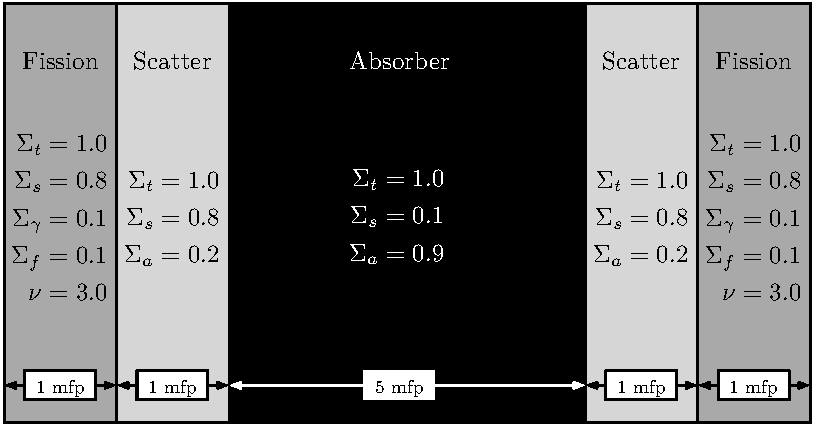
\includegraphics[width=\textwidth,keepaspectratio]{Figures/MultimediaCartoon}
    \caption{Diagram of heterogeneous slab geometry.  The symmetric simulation is shown in this figure.  For the asymmetric, heterogeneous simulation, the right-most region will have a width of 1.01 mfp.}
    \label{fig:HeteroGeometry}
\end{figure*}

The results for the asymmetric problem are shown first in Figure \ref{fig:Asymmetric}; the power method results are shown in Figure \ref{fig:AsymmetricPower} and the results from Arnoldi's method are shown in Figure \ref{fig:AsymmetricArnoldi}.  As in the homogeneous results the dashed line shows the reference eigenvalue\cite{Kornreich:2002Semi--0} of \num[group-digits=false]{0.427425} or the Shannon entropy at the end of the simulation for the power method and the mean Shannon entropy for Arnoldi's method.

\begin{figure*}[h]\centering
    \subfloat[Power method.]{\label{fig:AsymmetricPower}% GNUPLOT: LaTeX picture with Postscript
\begingroup%
\makeatletter%
\newcommand{\GNUPLOTspecial}{%
  \@sanitize\catcode`\%=14\relax\special}%
\setlength{\unitlength}{0.0500bp}%
\begin{picture}(8640,5760)(0,0)%
  {\GNUPLOTspecial{"
%!PS-Adobe-2.0 EPSF-2.0
%%Title: AsymmetricPower.tex
%%Creator: gnuplot 4.4 patchlevel 0
%%CreationDate: Wed Jul 28 09:34:07 2010
%%DocumentFonts: 
%%BoundingBox: 0 0 432 288
%%EndComments
%%BeginProlog
/gnudict 256 dict def
gnudict begin
%
% The following true/false flags may be edited by hand if desired.
% The unit line width and grayscale image gamma correction may also be changed.
%
/Color false def
/Blacktext true def
/Solid false def
/Dashlength 1 def
/Landscape false def
/Level1 false def
/Rounded false def
/ClipToBoundingBox false def
/TransparentPatterns false def
/gnulinewidth 5.000 def
/userlinewidth gnulinewidth def
/Gamma 1.0 def
%
/vshift -66 def
/dl1 {
  10.0 Dashlength mul mul
  Rounded { currentlinewidth 0.75 mul sub dup 0 le { pop 0.01 } if } if
} def
/dl2 {
  10.0 Dashlength mul mul
  Rounded { currentlinewidth 0.75 mul add } if
} def
/hpt_ 31.5 def
/vpt_ 31.5 def
/hpt hpt_ def
/vpt vpt_ def
Level1 {} {
/SDict 10 dict def
systemdict /pdfmark known not {
  userdict /pdfmark systemdict /cleartomark get put
} if
SDict begin [
  /Title (AsymmetricPower.tex)
  /Subject (gnuplot plot)
  /Creator (gnuplot 4.4 patchlevel 0)
  /Author (jlconlin)
%  /Producer (gnuplot)
%  /Keywords ()
  /CreationDate (Wed Jul 28 09:34:07 2010)
  /DOCINFO pdfmark
end
} ifelse
/doclip {
  ClipToBoundingBox {
    newpath 0 0 moveto 432 0 lineto 432 288 lineto 0 288 lineto closepath
    clip
  } if
} def
%
% Gnuplot Prolog Version 4.4 (January 2010)
%
%/SuppressPDFMark true def
%
/M {moveto} bind def
/L {lineto} bind def
/R {rmoveto} bind def
/V {rlineto} bind def
/N {newpath moveto} bind def
/Z {closepath} bind def
/C {setrgbcolor} bind def
/f {rlineto fill} bind def
/Gshow {show} def   % May be redefined later in the file to support UTF-8
/vpt2 vpt 2 mul def
/hpt2 hpt 2 mul def
/Lshow {currentpoint stroke M 0 vshift R 
	Blacktext {gsave 0 setgray show grestore} {show} ifelse} def
/Rshow {currentpoint stroke M dup stringwidth pop neg vshift R
	Blacktext {gsave 0 setgray show grestore} {show} ifelse} def
/Cshow {currentpoint stroke M dup stringwidth pop -2 div vshift R 
	Blacktext {gsave 0 setgray show grestore} {show} ifelse} def
/UP {dup vpt_ mul /vpt exch def hpt_ mul /hpt exch def
  /hpt2 hpt 2 mul def /vpt2 vpt 2 mul def} def
/DL {Color {setrgbcolor Solid {pop []} if 0 setdash}
 {pop pop pop 0 setgray Solid {pop []} if 0 setdash} ifelse} def
/BL {stroke userlinewidth 2 mul setlinewidth
	Rounded {1 setlinejoin 1 setlinecap} if} def
/AL {stroke userlinewidth 2 div setlinewidth
	Rounded {1 setlinejoin 1 setlinecap} if} def
/UL {dup gnulinewidth mul /userlinewidth exch def
	dup 1 lt {pop 1} if 10 mul /udl exch def} def
/PL {stroke userlinewidth setlinewidth
	Rounded {1 setlinejoin 1 setlinecap} if} def
% Default Line colors
/LCw {1 1 1} def
/LCb {0 0 0} def
/LCa {0 0 0} def
/LC0 {1 0 0} def
/LC1 {0 1 0} def
/LC2 {0 0 1} def
/LC3 {1 0 1} def
/LC4 {0 1 1} def
/LC5 {1 1 0} def
/LC6 {0 0 0} def
/LC7 {1 0.3 0} def
/LC8 {0.5 0.5 0.5} def
% Default Line Types
/LTw {PL [] 1 setgray} def
/LTb {BL [] LCb DL} def
/LTa {AL [1 udl mul 2 udl mul] 0 setdash LCa setrgbcolor} def
/LT0 {PL [] LC0 DL} def
/LT1 {PL [4 dl1 2 dl2] LC1 DL} def
/LT2 {PL [2 dl1 3 dl2] LC2 DL} def
/LT3 {PL [1 dl1 1.5 dl2] LC3 DL} def
/LT4 {PL [6 dl1 2 dl2 1 dl1 2 dl2] LC4 DL} def
/LT5 {PL [3 dl1 3 dl2 1 dl1 3 dl2] LC5 DL} def
/LT6 {PL [2 dl1 2 dl2 2 dl1 6 dl2] LC6 DL} def
/LT7 {PL [1 dl1 2 dl2 6 dl1 2 dl2 1 dl1 2 dl2] LC7 DL} def
/LT8 {PL [2 dl1 2 dl2 2 dl1 2 dl2 2 dl1 2 dl2 2 dl1 4 dl2] LC8 DL} def
/Pnt {stroke [] 0 setdash gsave 1 setlinecap M 0 0 V stroke grestore} def
/Dia {stroke [] 0 setdash 2 copy vpt add M
  hpt neg vpt neg V hpt vpt neg V
  hpt vpt V hpt neg vpt V closepath stroke
  Pnt} def
/Pls {stroke [] 0 setdash vpt sub M 0 vpt2 V
  currentpoint stroke M
  hpt neg vpt neg R hpt2 0 V stroke
 } def
/Box {stroke [] 0 setdash 2 copy exch hpt sub exch vpt add M
  0 vpt2 neg V hpt2 0 V 0 vpt2 V
  hpt2 neg 0 V closepath stroke
  Pnt} def
/Crs {stroke [] 0 setdash exch hpt sub exch vpt add M
  hpt2 vpt2 neg V currentpoint stroke M
  hpt2 neg 0 R hpt2 vpt2 V stroke} def
/TriU {stroke [] 0 setdash 2 copy vpt 1.12 mul add M
  hpt neg vpt -1.62 mul V
  hpt 2 mul 0 V
  hpt neg vpt 1.62 mul V closepath stroke
  Pnt} def
/Star {2 copy Pls Crs} def
/BoxF {stroke [] 0 setdash exch hpt sub exch vpt add M
  0 vpt2 neg V hpt2 0 V 0 vpt2 V
  hpt2 neg 0 V closepath fill} def
/TriUF {stroke [] 0 setdash vpt 1.12 mul add M
  hpt neg vpt -1.62 mul V
  hpt 2 mul 0 V
  hpt neg vpt 1.62 mul V closepath fill} def
/TriD {stroke [] 0 setdash 2 copy vpt 1.12 mul sub M
  hpt neg vpt 1.62 mul V
  hpt 2 mul 0 V
  hpt neg vpt -1.62 mul V closepath stroke
  Pnt} def
/TriDF {stroke [] 0 setdash vpt 1.12 mul sub M
  hpt neg vpt 1.62 mul V
  hpt 2 mul 0 V
  hpt neg vpt -1.62 mul V closepath fill} def
/DiaF {stroke [] 0 setdash vpt add M
  hpt neg vpt neg V hpt vpt neg V
  hpt vpt V hpt neg vpt V closepath fill} def
/Pent {stroke [] 0 setdash 2 copy gsave
  translate 0 hpt M 4 {72 rotate 0 hpt L} repeat
  closepath stroke grestore Pnt} def
/PentF {stroke [] 0 setdash gsave
  translate 0 hpt M 4 {72 rotate 0 hpt L} repeat
  closepath fill grestore} def
/Circle {stroke [] 0 setdash 2 copy
  hpt 0 360 arc stroke Pnt} def
/CircleF {stroke [] 0 setdash hpt 0 360 arc fill} def
/C0 {BL [] 0 setdash 2 copy moveto vpt 90 450 arc} bind def
/C1 {BL [] 0 setdash 2 copy moveto
	2 copy vpt 0 90 arc closepath fill
	vpt 0 360 arc closepath} bind def
/C2 {BL [] 0 setdash 2 copy moveto
	2 copy vpt 90 180 arc closepath fill
	vpt 0 360 arc closepath} bind def
/C3 {BL [] 0 setdash 2 copy moveto
	2 copy vpt 0 180 arc closepath fill
	vpt 0 360 arc closepath} bind def
/C4 {BL [] 0 setdash 2 copy moveto
	2 copy vpt 180 270 arc closepath fill
	vpt 0 360 arc closepath} bind def
/C5 {BL [] 0 setdash 2 copy moveto
	2 copy vpt 0 90 arc
	2 copy moveto
	2 copy vpt 180 270 arc closepath fill
	vpt 0 360 arc} bind def
/C6 {BL [] 0 setdash 2 copy moveto
	2 copy vpt 90 270 arc closepath fill
	vpt 0 360 arc closepath} bind def
/C7 {BL [] 0 setdash 2 copy moveto
	2 copy vpt 0 270 arc closepath fill
	vpt 0 360 arc closepath} bind def
/C8 {BL [] 0 setdash 2 copy moveto
	2 copy vpt 270 360 arc closepath fill
	vpt 0 360 arc closepath} bind def
/C9 {BL [] 0 setdash 2 copy moveto
	2 copy vpt 270 450 arc closepath fill
	vpt 0 360 arc closepath} bind def
/C10 {BL [] 0 setdash 2 copy 2 copy moveto vpt 270 360 arc closepath fill
	2 copy moveto
	2 copy vpt 90 180 arc closepath fill
	vpt 0 360 arc closepath} bind def
/C11 {BL [] 0 setdash 2 copy moveto
	2 copy vpt 0 180 arc closepath fill
	2 copy moveto
	2 copy vpt 270 360 arc closepath fill
	vpt 0 360 arc closepath} bind def
/C12 {BL [] 0 setdash 2 copy moveto
	2 copy vpt 180 360 arc closepath fill
	vpt 0 360 arc closepath} bind def
/C13 {BL [] 0 setdash 2 copy moveto
	2 copy vpt 0 90 arc closepath fill
	2 copy moveto
	2 copy vpt 180 360 arc closepath fill
	vpt 0 360 arc closepath} bind def
/C14 {BL [] 0 setdash 2 copy moveto
	2 copy vpt 90 360 arc closepath fill
	vpt 0 360 arc} bind def
/C15 {BL [] 0 setdash 2 copy vpt 0 360 arc closepath fill
	vpt 0 360 arc closepath} bind def
/Rec {newpath 4 2 roll moveto 1 index 0 rlineto 0 exch rlineto
	neg 0 rlineto closepath} bind def
/Square {dup Rec} bind def
/Bsquare {vpt sub exch vpt sub exch vpt2 Square} bind def
/S0 {BL [] 0 setdash 2 copy moveto 0 vpt rlineto BL Bsquare} bind def
/S1 {BL [] 0 setdash 2 copy vpt Square fill Bsquare} bind def
/S2 {BL [] 0 setdash 2 copy exch vpt sub exch vpt Square fill Bsquare} bind def
/S3 {BL [] 0 setdash 2 copy exch vpt sub exch vpt2 vpt Rec fill Bsquare} bind def
/S4 {BL [] 0 setdash 2 copy exch vpt sub exch vpt sub vpt Square fill Bsquare} bind def
/S5 {BL [] 0 setdash 2 copy 2 copy vpt Square fill
	exch vpt sub exch vpt sub vpt Square fill Bsquare} bind def
/S6 {BL [] 0 setdash 2 copy exch vpt sub exch vpt sub vpt vpt2 Rec fill Bsquare} bind def
/S7 {BL [] 0 setdash 2 copy exch vpt sub exch vpt sub vpt vpt2 Rec fill
	2 copy vpt Square fill Bsquare} bind def
/S8 {BL [] 0 setdash 2 copy vpt sub vpt Square fill Bsquare} bind def
/S9 {BL [] 0 setdash 2 copy vpt sub vpt vpt2 Rec fill Bsquare} bind def
/S10 {BL [] 0 setdash 2 copy vpt sub vpt Square fill 2 copy exch vpt sub exch vpt Square fill
	Bsquare} bind def
/S11 {BL [] 0 setdash 2 copy vpt sub vpt Square fill 2 copy exch vpt sub exch vpt2 vpt Rec fill
	Bsquare} bind def
/S12 {BL [] 0 setdash 2 copy exch vpt sub exch vpt sub vpt2 vpt Rec fill Bsquare} bind def
/S13 {BL [] 0 setdash 2 copy exch vpt sub exch vpt sub vpt2 vpt Rec fill
	2 copy vpt Square fill Bsquare} bind def
/S14 {BL [] 0 setdash 2 copy exch vpt sub exch vpt sub vpt2 vpt Rec fill
	2 copy exch vpt sub exch vpt Square fill Bsquare} bind def
/S15 {BL [] 0 setdash 2 copy Bsquare fill Bsquare} bind def
/D0 {gsave translate 45 rotate 0 0 S0 stroke grestore} bind def
/D1 {gsave translate 45 rotate 0 0 S1 stroke grestore} bind def
/D2 {gsave translate 45 rotate 0 0 S2 stroke grestore} bind def
/D3 {gsave translate 45 rotate 0 0 S3 stroke grestore} bind def
/D4 {gsave translate 45 rotate 0 0 S4 stroke grestore} bind def
/D5 {gsave translate 45 rotate 0 0 S5 stroke grestore} bind def
/D6 {gsave translate 45 rotate 0 0 S6 stroke grestore} bind def
/D7 {gsave translate 45 rotate 0 0 S7 stroke grestore} bind def
/D8 {gsave translate 45 rotate 0 0 S8 stroke grestore} bind def
/D9 {gsave translate 45 rotate 0 0 S9 stroke grestore} bind def
/D10 {gsave translate 45 rotate 0 0 S10 stroke grestore} bind def
/D11 {gsave translate 45 rotate 0 0 S11 stroke grestore} bind def
/D12 {gsave translate 45 rotate 0 0 S12 stroke grestore} bind def
/D13 {gsave translate 45 rotate 0 0 S13 stroke grestore} bind def
/D14 {gsave translate 45 rotate 0 0 S14 stroke grestore} bind def
/D15 {gsave translate 45 rotate 0 0 S15 stroke grestore} bind def
/DiaE {stroke [] 0 setdash vpt add M
  hpt neg vpt neg V hpt vpt neg V
  hpt vpt V hpt neg vpt V closepath stroke} def
/BoxE {stroke [] 0 setdash exch hpt sub exch vpt add M
  0 vpt2 neg V hpt2 0 V 0 vpt2 V
  hpt2 neg 0 V closepath stroke} def
/TriUE {stroke [] 0 setdash vpt 1.12 mul add M
  hpt neg vpt -1.62 mul V
  hpt 2 mul 0 V
  hpt neg vpt 1.62 mul V closepath stroke} def
/TriDE {stroke [] 0 setdash vpt 1.12 mul sub M
  hpt neg vpt 1.62 mul V
  hpt 2 mul 0 V
  hpt neg vpt -1.62 mul V closepath stroke} def
/PentE {stroke [] 0 setdash gsave
  translate 0 hpt M 4 {72 rotate 0 hpt L} repeat
  closepath stroke grestore} def
/CircE {stroke [] 0 setdash 
  hpt 0 360 arc stroke} def
/Opaque {gsave closepath 1 setgray fill grestore 0 setgray closepath} def
/DiaW {stroke [] 0 setdash vpt add M
  hpt neg vpt neg V hpt vpt neg V
  hpt vpt V hpt neg vpt V Opaque stroke} def
/BoxW {stroke [] 0 setdash exch hpt sub exch vpt add M
  0 vpt2 neg V hpt2 0 V 0 vpt2 V
  hpt2 neg 0 V Opaque stroke} def
/TriUW {stroke [] 0 setdash vpt 1.12 mul add M
  hpt neg vpt -1.62 mul V
  hpt 2 mul 0 V
  hpt neg vpt 1.62 mul V Opaque stroke} def
/TriDW {stroke [] 0 setdash vpt 1.12 mul sub M
  hpt neg vpt 1.62 mul V
  hpt 2 mul 0 V
  hpt neg vpt -1.62 mul V Opaque stroke} def
/PentW {stroke [] 0 setdash gsave
  translate 0 hpt M 4 {72 rotate 0 hpt L} repeat
  Opaque stroke grestore} def
/CircW {stroke [] 0 setdash 
  hpt 0 360 arc Opaque stroke} def
/BoxFill {gsave Rec 1 setgray fill grestore} def
/Density {
  /Fillden exch def
  currentrgbcolor
  /ColB exch def /ColG exch def /ColR exch def
  /ColR ColR Fillden mul Fillden sub 1 add def
  /ColG ColG Fillden mul Fillden sub 1 add def
  /ColB ColB Fillden mul Fillden sub 1 add def
  ColR ColG ColB setrgbcolor} def
/BoxColFill {gsave Rec PolyFill} def
/PolyFill {gsave Density fill grestore grestore} def
/h {rlineto rlineto rlineto gsave closepath fill grestore} bind def
%
% PostScript Level 1 Pattern Fill routine for rectangles
% Usage: x y w h s a XX PatternFill
%	x,y = lower left corner of box to be filled
%	w,h = width and height of box
%	  a = angle in degrees between lines and x-axis
%	 XX = 0/1 for no/yes cross-hatch
%
/PatternFill {gsave /PFa [ 9 2 roll ] def
  PFa 0 get PFa 2 get 2 div add PFa 1 get PFa 3 get 2 div add translate
  PFa 2 get -2 div PFa 3 get -2 div PFa 2 get PFa 3 get Rec
  gsave 1 setgray fill grestore clip
  currentlinewidth 0.5 mul setlinewidth
  /PFs PFa 2 get dup mul PFa 3 get dup mul add sqrt def
  0 0 M PFa 5 get rotate PFs -2 div dup translate
  0 1 PFs PFa 4 get div 1 add floor cvi
	{PFa 4 get mul 0 M 0 PFs V} for
  0 PFa 6 get ne {
	0 1 PFs PFa 4 get div 1 add floor cvi
	{PFa 4 get mul 0 2 1 roll M PFs 0 V} for
 } if
  stroke grestore} def
%
/languagelevel where
 {pop languagelevel} {1} ifelse
 2 lt
	{/InterpretLevel1 true def}
	{/InterpretLevel1 Level1 def}
 ifelse
%
% PostScript level 2 pattern fill definitions
%
/Level2PatternFill {
/Tile8x8 {/PaintType 2 /PatternType 1 /TilingType 1 /BBox [0 0 8 8] /XStep 8 /YStep 8}
	bind def
/KeepColor {currentrgbcolor [/Pattern /DeviceRGB] setcolorspace} bind def
<< Tile8x8
 /PaintProc {0.5 setlinewidth pop 0 0 M 8 8 L 0 8 M 8 0 L stroke} 
>> matrix makepattern
/Pat1 exch def
<< Tile8x8
 /PaintProc {0.5 setlinewidth pop 0 0 M 8 8 L 0 8 M 8 0 L stroke
	0 4 M 4 8 L 8 4 L 4 0 L 0 4 L stroke}
>> matrix makepattern
/Pat2 exch def
<< Tile8x8
 /PaintProc {0.5 setlinewidth pop 0 0 M 0 8 L
	8 8 L 8 0 L 0 0 L fill}
>> matrix makepattern
/Pat3 exch def
<< Tile8x8
 /PaintProc {0.5 setlinewidth pop -4 8 M 8 -4 L
	0 12 M 12 0 L stroke}
>> matrix makepattern
/Pat4 exch def
<< Tile8x8
 /PaintProc {0.5 setlinewidth pop -4 0 M 8 12 L
	0 -4 M 12 8 L stroke}
>> matrix makepattern
/Pat5 exch def
<< Tile8x8
 /PaintProc {0.5 setlinewidth pop -2 8 M 4 -4 L
	0 12 M 8 -4 L 4 12 M 10 0 L stroke}
>> matrix makepattern
/Pat6 exch def
<< Tile8x8
 /PaintProc {0.5 setlinewidth pop -2 0 M 4 12 L
	0 -4 M 8 12 L 4 -4 M 10 8 L stroke}
>> matrix makepattern
/Pat7 exch def
<< Tile8x8
 /PaintProc {0.5 setlinewidth pop 8 -2 M -4 4 L
	12 0 M -4 8 L 12 4 M 0 10 L stroke}
>> matrix makepattern
/Pat8 exch def
<< Tile8x8
 /PaintProc {0.5 setlinewidth pop 0 -2 M 12 4 L
	-4 0 M 12 8 L -4 4 M 8 10 L stroke}
>> matrix makepattern
/Pat9 exch def
/Pattern1 {PatternBgnd KeepColor Pat1 setpattern} bind def
/Pattern2 {PatternBgnd KeepColor Pat2 setpattern} bind def
/Pattern3 {PatternBgnd KeepColor Pat3 setpattern} bind def
/Pattern4 {PatternBgnd KeepColor Landscape {Pat5} {Pat4} ifelse setpattern} bind def
/Pattern5 {PatternBgnd KeepColor Landscape {Pat4} {Pat5} ifelse setpattern} bind def
/Pattern6 {PatternBgnd KeepColor Landscape {Pat9} {Pat6} ifelse setpattern} bind def
/Pattern7 {PatternBgnd KeepColor Landscape {Pat8} {Pat7} ifelse setpattern} bind def
} def
%
%
%End of PostScript Level 2 code
%
/PatternBgnd {
  TransparentPatterns {} {gsave 1 setgray fill grestore} ifelse
} def
%
% Substitute for Level 2 pattern fill codes with
% grayscale if Level 2 support is not selected.
%
/Level1PatternFill {
/Pattern1 {0.250 Density} bind def
/Pattern2 {0.500 Density} bind def
/Pattern3 {0.750 Density} bind def
/Pattern4 {0.125 Density} bind def
/Pattern5 {0.375 Density} bind def
/Pattern6 {0.625 Density} bind def
/Pattern7 {0.875 Density} bind def
} def
%
% Now test for support of Level 2 code
%
Level1 {Level1PatternFill} {Level2PatternFill} ifelse
%
/Symbol-Oblique /Symbol findfont [1 0 .167 1 0 0] makefont
dup length dict begin {1 index /FID eq {pop pop} {def} ifelse} forall
currentdict end definefont pop
end
%%EndProlog
gnudict begin
gsave
doclip
0 0 translate
0.050 0.050 scale
0 setgray
newpath
1.000 UL
LTb
1340 640 M
63 0 V
-63 813 R
63 0 V
-63 813 R
63 0 V
-63 814 R
63 0 V
-63 813 R
63 0 V
-63 813 R
63 0 V
-63 813 R
63 0 V
1340 640 M
0 63 V
0 4816 R
0 -63 V
1948 640 M
0 63 V
0 4816 R
0 -63 V
2556 640 M
0 63 V
0 4816 R
0 -63 V
3164 640 M
0 63 V
0 4816 R
0 -63 V
3772 640 M
0 63 V
0 4816 R
0 -63 V
4380 640 M
0 63 V
0 4816 R
0 -63 V
4987 640 M
0 63 V
0 4816 R
0 -63 V
5595 640 M
0 63 V
0 4816 R
0 -63 V
6203 640 M
0 63 V
0 4816 R
0 -63 V
6811 640 M
0 63 V
0 4816 R
0 -63 V
7419 640 M
0 63 V
0 4816 R
0 -63 V
0 -4816 R
-63 0 V
63 542 R
-63 0 V
63 542 R
-63 0 V
63 542 R
-63 0 V
63 542 R
-63 0 V
63 543 R
-63 0 V
63 542 R
-63 0 V
63 542 R
-63 0 V
63 542 R
-63 0 V
63 542 R
-63 0 V
stroke
1340 5519 N
0 -4879 V
6079 0 V
0 4879 V
-6079 0 V
Z stroke
LCb setrgbcolor
LTb
LCb setrgbcolor
LTb
LCb setrgbcolor
LTb
LCb setrgbcolor
LTb
1.000 UP
1.000 UL
LTb
1.000 UL
LT0
1342 640 M
3 3116 V
2 678 V
3 139 V
2 -58 V
3 -171 V
2 474 V
2 -313 V
3 131 V
2 -18 V
3 83 V
2 -31 V
3 -48 V
2 19 V
2 65 V
3 -31 V
2 -16 V
3 -164 V
2 98 V
3 51 V
2 50 V
2 -7 V
3 -43 V
2 -31 V
3 -102 V
2 65 V
3 121 V
2 -290 V
3 47 V
2 138 V
2 52 V
3 9 V
2 3 V
3 -175 V
2 22 V
3 125 V
2 8 V
2 17 V
3 -215 V
2 243 V
3 124 V
2 -296 V
3 153 V
2 29 V
2 -30 V
3 -78 V
2 67 V
3 -209 V
2 38 V
3 221 V
2 22 V
2 -89 V
3 -173 V
2 236 V
3 -20 V
2 -276 V
3 191 V
2 17 V
2 11 V
3 -121 V
2 64 V
3 181 V
2 -106 V
3 15 V
2 -136 V
2 -28 V
3 185 V
2 -231 V
3 184 V
2 49 V
3 -272 V
2 12 V
3 161 V
2 11 V
2 6 V
3 17 V
2 -100 V
3 120 V
2 -63 V
3 20 V
2 146 V
2 -128 V
3 -11 V
2 22 V
3 -127 V
2 336 V
3 -213 V
2 -7 V
2 -41 V
3 100 V
2 -217 V
3 257 V
2 -146 V
3 -70 V
2 226 V
2 -65 V
3 126 V
2 -217 V
3 219 V
2 -14 V
3 -123 V
2 -236 V
2 198 V
3 -32 V
2 133 V
stroke 1595 4703 M
3 -73 V
2 -54 V
3 -1 V
2 15 V
2 -28 V
3 117 V
2 25 V
3 -41 V
2 -95 V
3 137 V
2 11 V
2 -35 V
3 17 V
2 -52 V
3 137 V
2 -6 V
3 -56 V
2 -59 V
3 110 V
2 -98 V
2 5 V
3 -35 V
2 75 V
3 -266 V
2 157 V
3 6 V
2 -49 V
2 -70 V
3 24 V
2 182 V
3 -259 V
2 96 V
3 60 V
2 23 V
2 -74 V
3 194 V
2 -96 V
3 46 V
2 -196 V
3 141 V
2 -240 V
2 170 V
3 193 V
2 -54 V
3 -130 V
2 -21 V
3 239 V
2 -186 V
2 -10 V
3 87 V
2 14 V
3 -198 V
2 129 V
3 -12 V
2 115 V
2 -49 V
3 -123 V
2 21 V
3 -47 V
2 82 V
3 -69 V
2 27 V
3 47 V
2 0 V
2 169 V
3 -83 V
2 9 V
3 -212 V
2 8 V
3 78 V
2 49 V
2 -134 V
3 268 V
2 -80 V
3 -152 V
2 150 V
3 -235 V
2 356 V
2 -51 V
3 -197 V
2 57 V
3 -78 V
2 214 V
3 -320 V
2 184 V
2 108 V
3 -237 V
2 170 V
3 22 V
2 -56 V
3 68 V
2 26 V
2 -86 V
3 -13 V
2 -126 V
3 102 V
2 101 V
3 42 V
2 -234 V
2 356 V
3 -268 V
2 116 V
3 -93 V
2 -91 V
stroke 1848 4530 M
3 159 V
2 66 V
2 -184 V
3 139 V
2 -204 V
3 218 V
2 67 V
3 -204 V
2 47 V
3 -58 V
2 14 V
2 68 V
3 78 V
2 -83 V
3 -3 V
2 -53 V
3 43 V
2 34 V
2 -9 V
3 -48 V
2 -33 V
3 -9 V
2 205 V
3 -195 V
2 22 V
2 -78 V
3 173 V
2 63 V
3 35 V
2 -287 V
3 63 V
2 38 V
2 46 V
3 -61 V
2 -59 V
3 53 V
2 11 V
3 82 V
2 23 V
2 -28 V
3 53 V
2 -24 V
3 -74 V
2 24 V
3 0 V
2 -1 V
2 -117 V
3 152 V
2 -79 V
3 138 V
2 -181 V
3 128 V
2 -90 V
3 51 V
2 -113 V
2 127 V
3 68 V
2 85 V
3 -134 V
2 57 V
3 -154 V
2 121 V
2 -47 V
3 -37 V
2 133 V
3 -11 V
2 -64 V
3 -75 V
2 1 V
2 140 V
3 15 V
2 -65 V
3 -102 V
2 265 V
3 -307 V
2 171 V
2 51 V
3 -91 V
2 -15 V
3 -74 V
2 120 V
3 8 V
2 -89 V
2 194 V
3 23 V
2 -126 V
3 27 V
2 -136 V
3 126 V
2 -60 V
2 -162 V
3 83 V
2 105 V
3 -265 V
2 234 V
3 5 V
2 -26 V
3 101 V
2 -81 V
2 -108 V
3 12 V
2 -69 V
3 346 V
2 -200 V
stroke 2101 4668 M
3 85 V
2 -33 V
2 79 V
3 -101 V
2 -112 V
3 150 V
2 59 V
3 -158 V
2 -32 V
2 204 V
3 -35 V
2 12 V
3 -143 V
2 -29 V
3 193 V
2 -68 V
2 63 V
3 -116 V
2 -98 V
3 32 V
2 220 V
3 -120 V
2 43 V
2 81 V
3 -78 V
2 23 V
3 -55 V
2 36 V
3 15 V
2 -27 V
2 -3 V
3 -158 V
2 191 V
3 -36 V
2 -59 V
3 -38 V
2 39 V
2 -29 V
3 11 V
2 31 V
3 78 V
2 -87 V
3 -7 V
2 108 V
3 -55 V
2 13 V
2 11 V
3 -49 V
2 106 V
3 -140 V
2 -60 V
3 144 V
2 -18 V
2 58 V
3 21 V
2 -158 V
3 123 V
2 7 V
3 -150 V
2 142 V
2 -78 V
3 83 V
2 -89 V
3 31 V
2 -124 V
3 173 V
2 -110 V
2 17 V
3 -37 V
2 103 V
3 6 V
2 34 V
3 18 V
2 -34 V
2 -99 V
3 50 V
2 44 V
3 -33 V
2 28 V
3 54 V
2 70 V
2 -67 V
3 -227 V
2 210 V
3 8 V
2 -8 V
3 -18 V
2 -175 V
3 161 V
2 118 V
2 -81 V
3 26 V
2 -205 V
3 77 V
2 -69 V
3 61 V
2 116 V
2 -21 V
3 -97 V
2 88 V
3 -32 V
2 31 V
3 -134 V
2 203 V
stroke 2354 4866 M
2 -152 V
3 72 V
2 -28 V
3 99 V
2 -99 V
3 142 V
2 -148 V
2 -23 V
3 -95 V
2 193 V
3 -126 V
2 110 V
3 19 V
2 -99 V
2 75 V
3 -35 V
2 -77 V
3 149 V
2 -4 V
3 -246 V
2 255 V
2 -194 V
3 123 V
2 102 V
3 -92 V
2 47 V
3 -38 V
2 -43 V
2 -162 V
3 88 V
2 184 V
3 -140 V
2 93 V
3 19 V
2 28 V
3 7 V
2 -187 V
2 254 V
3 -135 V
2 -91 V
3 146 V
2 -82 V
3 71 V
2 -84 V
2 125 V
3 -108 V
2 -189 V
3 222 V
2 10 V
3 -148 V
2 49 V
2 149 V
3 -81 V
2 158 V
3 -217 V
2 146 V
3 -158 V
2 196 V
2 -123 V
3 -77 V
2 -81 V
3 267 V
2 -138 V
3 -18 V
2 143 V
2 -78 V
3 43 V
2 -53 V
3 125 V
2 -170 V
3 77 V
2 -94 V
2 71 V
3 -71 V
2 308 V
3 -261 V
2 24 V
3 -17 V
2 73 V
3 90 V
2 -80 V
2 -177 V
3 152 V
2 -97 V
3 111 V
2 49 V
3 -132 V
2 125 V
2 31 V
3 -81 V
2 -57 V
3 150 V
2 -5 V
3 -91 V
2 -54 V
2 -192 V
3 318 V
2 -56 V
3 -97 V
2 212 V
3 -114 V
2 -111 V
2 44 V
3 -33 V
stroke 2607 4771 M
2 147 V
3 10 V
2 -49 V
3 83 V
2 -143 V
2 88 V
3 -31 V
2 58 V
3 10 V
2 -174 V
3 83 V
2 34 V
2 -161 V
3 81 V
2 20 V
3 -132 V
2 141 V
3 39 V
2 73 V
2 -121 V
3 90 V
2 66 V
3 14 V
2 -86 V
3 150 V
2 -22 V
3 -125 V
2 70 V
2 -20 V
3 -68 V
2 21 V
3 -6 V
2 -98 V
3 183 V
2 -62 V
2 -47 V
3 143 V
2 3 V
3 -144 V
2 -180 V
3 323 V
2 -31 V
2 -97 V
3 9 V
2 -11 V
3 19 V
2 -61 V
3 28 V
2 -1 V
2 -28 V
3 -5 V
2 82 V
3 39 V
2 32 V
3 38 V
2 -5 V
2 -145 V
3 -187 V
2 281 V
3 -8 V
2 -10 V
3 -17 V
2 73 V
2 -301 V
3 218 V
2 115 V
3 -70 V
2 -52 V
3 33 V
2 19 V
3 -75 V
2 85 V
2 -245 V
3 144 V
2 160 V
3 -117 V
2 -30 V
3 -90 V
2 -19 V
2 230 V
3 -249 V
2 53 V
3 207 V
2 34 V
3 -188 V
2 97 V
2 135 V
3 -269 V
2 184 V
3 -155 V
2 51 V
3 17 V
2 -27 V
2 59 V
3 188 V
2 -378 V
3 50 V
2 -23 V
3 83 V
2 139 V
2 71 V
3 -134 V
2 121 V
3 -258 V
stroke 2860 4840 M
2 213 V
3 46 V
2 5 V
2 -196 V
3 -104 V
2 252 V
3 -255 V
2 55 V
3 307 V
2 -173 V
2 -3 V
3 88 V
2 -86 V
3 -4 V
2 123 V
3 -60 V
2 -34 V
3 -46 V
2 126 V
2 7 V
3 -138 V
2 87 V
3 -32 V
2 -278 V
3 232 V
2 -157 V
2 357 V
3 -43 V
2 -161 V
3 100 V
2 -259 V
3 175 V
2 194 V
2 -323 V
3 39 V
2 -9 V
3 306 V
2 -153 V
3 -8 V
2 -56 V
2 -114 V
3 288 V
2 -224 V
3 64 V
2 -3 V
3 -97 V
2 39 V
2 61 V
3 -4 V
2 134 V
3 -189 V
2 88 V
3 -91 V
2 56 V
2 137 V
3 -79 V
2 86 V
3 -69 V
2 -106 V
3 100 V
2 115 V
3 -93 V
2 -59 V
2 -33 V
3 -26 V
2 184 V
3 -212 V
2 -27 V
3 133 V
2 223 V
2 -335 V
3 292 V
2 -67 V
3 -183 V
2 37 V
3 -63 V
2 176 V
2 -228 V
3 186 V
2 -250 V
3 306 V
2 -129 V
3 -40 V
2 -9 V
2 -9 V
3 21 V
2 56 V
3 -18 V
2 -113 V
3 108 V
2 -162 V
2 195 V
3 264 V
2 -318 V
3 28 V
2 36 V
3 -112 V
2 11 V
2 93 V
3 167 V
2 -110 V
3 -100 V
2 38 V
3 -2 V
stroke 3113 5022 M
2 -37 V
2 9 V
3 -29 V
2 177 V
3 -88 V
2 36 V
3 -74 V
2 -148 V
3 97 V
2 143 V
2 -151 V
3 147 V
2 -179 V
3 69 V
2 245 V
3 -115 V
2 -157 V
2 38 V
3 -115 V
2 45 V
3 109 V
2 89 V
3 -221 V
2 123 V
2 -197 V
3 11 V
2 223 V
3 -243 V
2 133 V
3 -11 V
2 71 V
2 -62 V
3 -107 V
2 192 V
3 -45 V
2 32 V
3 37 V
2 -129 V
2 78 V
3 210 V
2 -153 V
3 -75 V
2 -32 V
3 332 V
2 -210 V
2 -60 V
3 120 V
2 -60 V
3 88 V
2 -123 V
3 57 V
2 -108 V
3 237 V
2 -97 V
2 -23 V
3 106 V
2 -131 V
3 -4 V
2 22 V
3 2 V
2 -67 V
2 64 V
3 59 V
2 -194 V
3 55 V
2 -108 V
3 100 V
2 -4 V
2 23 V
3 70 V
2 -74 V
3 15 V
2 -117 V
3 -27 V
2 153 V
2 -36 V
3 194 V
2 -181 V
3 -100 V
2 230 V
3 -143 V
2 -88 V
2 -13 V
3 142 V
2 30 V
3 -29 V
2 -189 V
3 33 V
2 230 V
2 61 V
3 -134 V
2 16 V
3 -31 V
2 -44 V
3 36 V
2 -87 V
3 33 V
2 91 V
2 139 V
3 -190 V
2 9 V
3 3 V
2 42 V
3 121 V
stroke 3366 5209 M
2 -105 V
2 -117 V
3 8 V
2 161 V
3 -138 V
2 101 V
3 -58 V
2 5 V
2 57 V
3 -127 V
2 150 V
3 -64 V
2 -137 V
3 -62 V
2 212 V
2 50 V
3 -100 V
2 156 V
3 -37 V
2 97 V
3 -186 V
2 -100 V
2 -46 V
3 48 V
2 143 V
3 -79 V
2 -12 V
3 -81 V
2 145 V
2 81 V
3 -141 V
2 81 V
3 -4 V
2 106 V
3 -119 V
2 -12 V
2 -88 V
3 108 V
2 -29 V
3 -96 V
2 156 V
3 66 V
2 -40 V
3 -117 V
2 29 V
2 7 V
3 -88 V
2 6 V
3 15 V
2 80 V
3 -56 V
2 -16 V
2 2 V
3 -42 V
2 13 V
3 101 V
2 -42 V
3 -146 V
2 211 V
2 32 V
3 -281 V
2 128 V
3 234 V
2 -321 V
3 166 V
2 66 V
2 -175 V
3 213 V
2 -5 V
3 -53 V
2 -50 V
3 -14 V
2 72 V
2 -143 V
3 103 V
2 -86 V
3 52 V
2 137 V
3 -83 V
2 -37 V
2 220 V
3 -84 V
2 -15 V
3 -161 V
2 5 V
3 3 V
2 -40 V
3 194 V
2 -11 V
2 -52 V
3 -76 V
2 228 V
3 -93 V
2 -85 V
3 -62 V
2 -22 V
2 153 V
3 -178 V
2 197 V
3 -184 V
2 84 V
3 59 V
2 26 V
2 -161 V
stroke 3618 5019 M
3 -29 V
2 96 V
3 57 V
2 -110 V
3 -189 V
2 220 V
2 48 V
3 -111 V
2 61 V
3 27 V
2 55 V
3 -30 V
2 -44 V
2 138 V
3 21 V
2 -190 V
3 114 V
2 114 V
3 -189 V
2 -72 V
2 246 V
3 -85 V
2 38 V
3 -128 V
2 142 V
3 -76 V
2 42 V
2 -157 V
3 153 V
2 -88 V
3 -173 V
2 85 V
3 84 V
2 -28 V
3 263 V
2 -120 V
2 -98 V
3 -85 V
2 327 V
3 -195 V
2 -119 V
3 168 V
2 80 V
2 -232 V
3 -33 V
2 -97 V
3 87 V
2 144 V
3 -124 V
2 83 V
2 136 V
3 -164 V
2 -115 V
3 -44 V
2 249 V
3 -83 V
2 58 V
2 -127 V
3 147 V
2 -28 V
3 156 V
2 -244 V
3 -30 V
2 13 V
2 48 V
3 8 V
2 -31 V
3 -38 V
2 129 V
3 -67 V
2 -85 V
2 97 V
3 -11 V
2 -57 V
3 -8 V
2 195 V
3 -100 V
2 -130 V
3 8 V
2 22 V
2 224 V
3 -177 V
2 56 V
3 -34 V
2 38 V
3 -95 V
2 202 V
2 -71 V
3 -8 V
2 -95 V
3 5 V
2 44 V
3 14 V
2 61 V
2 81 V
3 -236 V
2 181 V
3 -89 V
2 122 V
3 -256 V
2 275 V
2 -70 V
3 -147 V
2 96 V
stroke 3871 5135 M
3 55 V
2 -55 V
3 -28 V
2 -78 V
2 -18 V
3 158 V
2 -61 V
3 -14 V
2 -11 V
3 32 V
2 51 V
2 -42 V
3 -25 V
2 61 V
3 -226 V
2 167 V
3 113 V
2 -152 V
2 -173 V
3 186 V
2 81 V
3 -44 V
2 -44 V
3 188 V
2 -397 V
3 357 V
2 -79 V
2 -99 V
3 -16 V
2 -5 V
3 -8 V
2 94 V
3 -53 V
2 204 V
2 -158 V
3 -77 V
2 91 V
3 -61 V
2 102 V
3 92 V
2 1 V
2 -153 V
3 95 V
2 -108 V
3 31 V
2 245 V
3 -195 V
2 -169 V
2 154 V
3 15 V
2 60 V
3 -65 V
2 -34 V
3 -94 V
2 49 V
2 33 V
3 -142 V
2 151 V
3 -100 V
2 117 V
3 -74 V
2 -129 V
2 103 V
3 113 V
2 -99 V
3 -35 V
2 139 V
3 -240 V
2 163 V
3 121 V
2 -128 V
2 61 V
3 3 V
2 36 V
3 -68 V
2 -166 V
3 159 V
2 73 V
2 40 V
3 -80 V
2 -29 V
3 -62 V
2 117 V
3 -49 V
2 9 V
2 -138 V
3 5 V
2 149 V
3 -102 V
2 113 V
3 -24 V
2 41 V
2 -116 V
3 -50 V
2 37 V
3 45 V
2 -27 V
3 88 V
2 92 V
2 -58 V
3 -142 V
2 115 V
3 -5 V
2 36 V
stroke 4124 5171 M
3 -16 V
2 -5 V
2 70 V
3 75 V
2 -289 V
3 287 V
2 -247 V
3 49 V
2 -34 V
2 8 V
3 -102 V
2 169 V
3 -14 V
2 -121 V
3 20 V
2 29 V
3 128 V
2 -147 V
2 70 V
3 -59 V
2 30 V
3 -64 V
2 18 V
3 125 V
2 -128 V
2 73 V
3 -94 V
2 48 V
3 85 V
2 123 V
3 -145 V
2 -127 V
2 254 V
3 -48 V
2 -272 V
3 97 V
2 5 V
3 159 V
2 -113 V
2 -15 V
3 18 V
2 113 V
3 -36 V
2 -110 V
3 222 V
2 -131 V
2 -13 V
3 7 V
2 15 V
3 -81 V
2 112 V
3 -154 V
2 -51 V
2 113 V
3 -83 V
2 246 V
3 -150 V
2 26 V
3 -80 V
2 189 V
3 -245 V
2 68 V
2 -100 V
3 280 V
2 -33 V
3 -63 V
2 -39 V
3 -34 V
2 -95 V
2 189 V
3 161 V
2 -97 V
3 -74 V
2 -122 V
3 195 V
2 -103 V
2 19 V
3 -100 V
2 35 V
3 139 V
2 -11 V
3 -70 V
2 -162 V
2 182 V
3 -111 V
2 106 V
3 -77 V
2 -59 V
3 126 V
2 -1 V
2 196 V
3 -223 V
2 -156 V
3 188 V
2 -203 V
3 234 V
2 -12 V
2 -27 V
3 -172 V
2 176 V
3 7 V
2 -84 V
3 45 V
2 -33 V
stroke 4377 5065 M
3 -87 V
2 175 V
2 -40 V
3 -41 V
2 -41 V
3 -39 V
2 122 V
3 32 V
2 -97 V
2 -12 V
3 -3 V
2 -28 V
3 43 V
2 -2 V
3 -24 V
2 -24 V
2 -37 V
3 113 V
2 -90 V
3 243 V
2 -172 V
3 73 V
2 118 V
2 -126 V
3 -96 V
2 -52 V
3 112 V
2 19 V
3 51 V
2 -177 V
2 307 V
3 -160 V
2 48 V
3 46 V
2 -35 V
3 104 V
2 -324 V
2 239 V
3 -190 V
2 51 V
3 105 V
2 -243 V
3 229 V
2 -52 V
2 -10 V
3 -152 V
2 168 V
3 34 V
2 -113 V
3 204 V
2 -232 V
3 65 V
2 -59 V
2 231 V
3 -174 V
2 25 V
3 42 V
2 98 V
3 -74 V
2 -86 V
2 171 V
3 13 V
2 -95 V
3 -40 V
2 -125 V
3 125 V
2 30 V
2 36 V
3 -231 V
2 24 V
3 83 V
2 60 V
3 91 V
2 -242 V
2 89 V
3 -44 V
2 -90 V
3 315 V
2 -33 V
3 0 V
2 -254 V
2 96 V
3 114 V
2 3 V
3 -40 V
2 -103 V
3 -22 V
2 236 V
2 -119 V
3 -21 V
2 62 V
3 -53 V
2 -7 V
3 93 V
2 -121 V
3 -44 V
2 102 V
2 79 V
3 -146 V
2 45 V
3 147 V
2 -227 V
3 -10 V
2 47 V
stroke 4630 5064 M
2 -94 V
3 164 V
2 -81 V
3 17 V
2 -51 V
3 39 V
2 -20 V
2 -26 V
3 119 V
2 68 V
3 49 V
2 -191 V
3 155 V
2 -118 V
2 70 V
3 -99 V
2 -34 V
3 254 V
2 -252 V
3 133 V
2 -113 V
2 149 V
3 120 V
2 -260 V
3 -46 V
2 -4 V
3 177 V
2 31 V
2 -27 V
3 -14 V
2 -112 V
3 31 V
2 8 V
3 -71 V
2 189 V
2 -95 V
3 -13 V
2 107 V
3 -86 V
2 -41 V
3 -54 V
2 178 V
3 -187 V
2 80 V
2 -58 V
3 -83 V
2 156 V
3 -41 V
2 97 V
3 -325 V
2 290 V
2 -27 V
3 -138 V
2 127 V
3 48 V
2 -19 V
3 -166 V
2 14 V
2 213 V
3 -70 V
2 -132 V
3 116 V
2 -46 V
3 14 V
2 169 V
2 -254 V
3 42 V
2 10 V
3 -74 V
2 16 V
3 57 V
2 -111 V
2 80 V
3 51 V
2 -50 V
3 -5 V
2 117 V
3 -173 V
2 195 V
2 -144 V
3 14 V
2 214 V
3 -137 V
2 -39 V
3 -16 V
2 -109 V
3 39 V
2 178 V
2 -20 V
3 20 V
2 -52 V
3 23 V
2 37 V
3 -173 V
2 -48 V
2 137 V
3 143 V
2 -97 V
3 -10 V
2 -55 V
3 98 V
2 -173 V
2 145 V
3 -80 V
stroke 4883 5048 M
2 50 V
3 94 V
2 -89 V
3 75 V
2 -132 V
2 68 V
3 -28 V
2 1 V
3 -36 V
2 146 V
3 -156 V
2 104 V
2 12 V
3 -77 V
2 133 V
3 -91 V
2 0 V
3 3 V
2 225 V
2 -137 V
3 -122 V
2 -49 V
3 -16 V
2 -33 V
3 166 V
2 -167 V
2 180 V
3 -91 V
2 86 V
3 -53 V
2 127 V
3 -154 V
2 49 V
3 5 V
2 -149 V
2 194 V
3 -28 V
2 -74 V
3 -46 V
2 213 V
3 -166 V
2 150 V
2 -233 V
3 52 V
2 -8 V
3 48 V
2 11 V
3 -84 V
2 137 V
2 -157 V
3 157 V
2 -36 V
3 26 V
2 -108 V
3 96 V
2 -14 V
2 46 V
3 -99 V
2 174 V
3 239 V
2 -425 V
3 -88 V
2 38 V
2 -77 V
3 122 V
2 42 V
3 -29 V
2 209 V
3 -136 V
2 -145 V
2 51 V
3 6 V
2 154 V
3 -138 V
2 -38 V
3 40 V
2 20 V
3 171 V
2 -47 V
2 26 V
3 -346 V
2 174 V
3 88 V
2 -47 V
3 97 V
2 -172 V
2 48 V
3 158 V
2 -112 V
3 23 V
2 -45 V
3 129 V
2 -115 V
2 -6 V
3 93 V
2 -20 V
3 -3 V
2 -182 V
3 139 V
2 -70 V
2 123 V
3 -166 V
2 91 V
3 -170 V
stroke 5136 4947 M
2 145 V
3 -70 V
2 -7 V
2 287 V
3 -213 V
2 51 V
3 -74 V
2 -123 V
3 24 V
2 118 V
2 -19 V
3 81 V
2 56 V
3 -317 V
2 334 V
3 -50 V
2 79 V
2 -162 V
3 -45 V
2 113 V
3 35 V
2 -90 V
3 -114 V
2 94 V
3 132 V
2 -305 V
2 98 V
3 -16 V
2 153 V
3 -107 V
2 114 V
3 15 V
2 -217 V
2 172 V
3 100 V
2 -92 V
3 31 V
2 -91 V
3 131 V
2 -129 V
2 200 V
3 -174 V
2 59 V
3 -11 V
2 -85 V
3 128 V
2 -198 V
2 -55 V
3 141 V
2 -88 V
3 57 V
2 -94 V
3 88 V
2 -13 V
2 39 V
3 187 V
2 -145 V
3 -122 V
2 -92 V
3 218 V
2 29 V
2 -76 V
3 56 V
2 -21 V
3 25 V
2 52 V
3 -119 V
2 74 V
3 231 V
2 -401 V
2 262 V
3 27 V
2 -181 V
3 82 V
2 9 V
3 -56 V
2 -140 V
2 147 V
3 -22 V
2 82 V
3 -38 V
2 -31 V
3 -39 V
2 195 V
2 -277 V
3 106 V
2 101 V
3 -32 V
2 -93 V
3 -41 V
2 34 V
2 71 V
3 78 V
2 -62 V
3 -119 V
2 -24 V
3 203 V
2 -170 V
2 35 V
3 -35 V
2 49 V
3 -111 V
2 104 V
3 83 V
stroke 5389 5156 M
2 -141 V
2 107 V
3 -66 V
2 16 V
3 -66 V
2 76 V
3 -71 V
2 20 V
2 0 V
3 89 V
2 -106 V
3 -131 V
2 169 V
3 214 V
2 -196 V
3 -156 V
2 314 V
2 -98 V
3 167 V
2 -213 V
3 82 V
2 7 V
3 -57 V
2 33 V
2 0 V
3 -49 V
2 22 V
3 -4 V
2 -38 V
3 41 V
2 -97 V
2 91 V
3 -172 V
2 207 V
3 -130 V
2 75 V
3 205 V
2 -195 V
2 128 V
3 -163 V
2 87 V
3 -143 V
2 100 V
3 -29 V
2 115 V
2 -64 V
3 -183 V
2 202 V
3 -46 V
2 71 V
3 11 V
2 -256 V
2 167 V
3 184 V
2 -291 V
3 316 V
2 -319 V
3 -21 V
2 91 V
3 -54 V
2 249 V
2 2 V
3 -145 V
2 32 V
3 79 V
2 15 V
3 -84 V
2 51 V
2 24 V
3 -86 V
2 99 V
3 -127 V
2 27 V
3 -80 V
2 185 V
2 -219 V
3 -45 V
2 137 V
3 155 V
2 -31 V
3 -141 V
2 32 V
2 -36 V
3 -89 V
2 150 V
3 137 V
2 -159 V
3 -146 V
2 136 V
2 -6 V
3 14 V
2 -66 V
3 -144 V
2 216 V
3 -34 V
2 6 V
2 34 V
3 -6 V
2 -112 V
3 65 V
2 131 V
3 84 V
2 -210 V
3 0 V
stroke 5642 5102 M
2 -84 V
2 251 V
3 -221 V
2 73 V
3 -98 V
2 99 V
3 -111 V
2 18 V
2 72 V
3 85 V
2 -107 V
3 77 V
2 -4 V
3 98 V
2 -238 V
2 -136 V
3 219 V
2 141 V
3 -134 V
2 -8 V
3 -69 V
2 -39 V
2 -52 V
3 279 V
2 -117 V
3 -126 V
2 52 V
3 72 V
2 73 V
2 -21 V
3 -54 V
2 -11 V
3 46 V
2 -95 V
3 147 V
2 36 V
2 -6 V
3 -181 V
2 32 V
3 -16 V
2 121 V
3 71 V
2 -148 V
2 18 V
3 -122 V
2 75 V
3 12 V
2 189 V
3 -129 V
2 -64 V
3 79 V
2 -66 V
2 -51 V
3 84 V
2 -168 V
3 133 V
2 92 V
3 26 V
2 -196 V
2 123 V
3 -73 V
2 243 V
3 -136 V
2 36 V
3 -308 V
2 187 V
2 -96 V
3 146 V
2 -40 V
3 165 V
2 -153 V
3 43 V
2 -105 V
2 59 V
3 109 V
2 -190 V
3 193 V
2 -61 V
3 -77 V
2 -17 V
2 30 V
3 205 V
2 -26 V
3 -162 V
2 -100 V
3 -10 V
2 -26 V
2 5 V
3 199 V
2 -137 V
3 162 V
2 -106 V
3 80 V
2 -147 V
3 151 V
2 -16 V
2 -68 V
3 0 V
2 40 V
3 -202 V
2 286 V
3 -90 V
2 -53 V
2 108 V
stroke 5894 5171 M
3 -107 V
2 135 V
3 -136 V
2 58 V
3 -4 V
2 82 V
2 -50 V
3 -93 V
2 89 V
3 -123 V
2 123 V
3 -116 V
2 58 V
2 33 V
3 -2 V
2 -51 V
3 124 V
2 -84 V
3 -59 V
2 -49 V
2 -9 V
3 127 V
2 4 V
3 22 V
2 70 V
3 -52 V
2 -52 V
2 91 V
3 -138 V
2 125 V
3 -52 V
2 -10 V
3 -132 V
2 98 V
2 24 V
3 -36 V
2 86 V
3 -63 V
2 104 V
3 -106 V
2 -75 V
3 -7 V
2 19 V
2 13 V
3 -15 V
2 -102 V
3 149 V
2 14 V
3 70 V
2 -169 V
2 45 V
3 86 V
2 -87 V
3 -6 V
2 62 V
3 103 V
2 -173 V
2 108 V
3 -216 V
2 173 V
3 -79 V
2 125 V
3 -80 V
2 77 V
2 -150 V
3 73 V
2 -16 V
3 87 V
2 -106 V
3 35 V
2 7 V
2 40 V
3 -4 V
2 149 V
3 -233 V
2 159 V
3 -39 V
2 -38 V
2 -30 V
3 -77 V
2 284 V
3 -319 V
2 127 V
3 8 V
2 -13 V
3 -33 V
2 101 V
2 -24 V
3 17 V
2 -14 V
3 -60 V
2 151 V
3 68 V
2 -245 V
2 88 V
3 20 V
2 -123 V
3 124 V
2 -105 V
3 21 V
2 93 V
2 -287 V
3 183 V
2 185 V
stroke 6147 5239 M
3 -83 V
2 -76 V
3 196 V
2 -85 V
2 -213 V
3 139 V
2 93 V
3 -58 V
2 -147 V
3 196 V
2 -100 V
2 94 V
3 -153 V
2 132 V
3 -190 V
2 57 V
3 31 V
2 6 V
2 -75 V
3 10 V
2 92 V
3 -136 V
2 -24 V
3 79 V
2 51 V
2 -63 V
3 -15 V
2 144 V
3 -177 V
2 284 V
3 -142 V
2 84 V
3 -89 V
2 191 V
2 -186 V
3 -19 V
2 9 V
3 135 V
2 -91 V
3 -10 V
2 -15 V
2 15 V
3 -249 V
2 155 V
3 -12 V
2 15 V
3 -60 V
2 116 V
2 8 V
3 -141 V
2 141 V
3 -166 V
2 121 V
3 125 V
2 -175 V
2 152 V
3 5 V
2 2 V
3 -20 V
2 -89 V
3 -4 V
2 93 V
2 151 V
3 -303 V
2 68 V
3 -45 V
2 -23 V
3 171 V
2 75 V
2 36 V
3 -135 V
2 -132 V
3 49 V
2 168 V
3 -128 V
2 132 V
3 -117 V
2 26 V
2 104 V
3 -81 V
2 -4 V
3 -169 V
2 42 V
3 41 V
2 179 V
2 -285 V
3 166 V
2 -113 V
3 110 V
2 -96 V
3 69 V
2 -44 V
2 131 V
3 2 V
2 -178 V
3 49 V
2 7 V
3 -77 V
2 128 V
2 -266 V
3 237 V
2 -193 V
3 201 V
2 -53 V
stroke 6400 5047 M
3 82 V
2 123 V
2 -232 V
3 217 V
2 3 V
3 -113 V
2 -30 V
3 -40 V
2 261 V
2 -156 V
3 -115 V
2 97 V
3 -250 V
2 270 V
3 -21 V
2 -82 V
2 31 V
3 45 V
2 -31 V
3 124 V
2 -191 V
3 84 V
2 26 V
3 -22 V
2 -107 V
2 176 V
3 -11 V
2 -103 V
3 -48 V
2 92 V
3 -21 V
2 -2 V
2 21 V
3 -60 V
2 -22 V
3 59 V
2 -180 V
3 119 V
2 -43 V
2 142 V
3 -47 V
2 -53 V
3 48 V
2 -82 V
3 -87 V
2 44 V
2 243 V
3 -36 V
2 -127 V
3 37 V
2 70 V
3 -104 V
2 145 V
2 -154 V
3 50 V
2 -62 V
3 56 V
2 108 V
3 -72 V
2 -70 V
2 59 V
3 23 V
2 5 V
3 -16 V
2 43 V
3 42 V
2 -58 V
3 118 V
2 -99 V
2 -117 V
3 -79 V
2 56 V
3 142 V
2 -42 V
3 111 V
2 -148 V
2 6 V
3 -96 V
2 87 V
3 -78 V
2 -19 V
3 175 V
2 -24 V
2 -164 V
3 136 V
2 151 V
3 -125 V
2 -157 V
3 121 V
2 -180 V
2 312 V
3 -122 V
2 -53 V
3 -58 V
2 168 V
3 -19 V
2 -29 V
2 142 V
3 -294 V
2 228 V
3 -15 V
2 -68 V
3 99 V
2 11 V
stroke 6653 5221 M
2 -168 V
3 58 V
2 -25 V
3 -83 V
2 -11 V
3 -139 V
2 328 V
2 97 V
3 -261 V
2 73 V
3 186 V
2 -300 V
3 83 V
2 97 V
3 -136 V
2 -114 V
2 143 V
3 171 V
2 -199 V
3 -21 V
2 152 V
3 25 V
2 -149 V
2 -76 V
3 53 V
2 261 V
3 -50 V
2 -142 V
3 94 V
2 -44 V
2 -125 V
3 83 V
2 142 V
3 -150 V
2 123 V
3 -101 V
2 93 V
2 -31 V
3 -119 V
2 -8 V
3 78 V
2 -50 V
3 68 V
2 -27 V
2 -136 V
3 114 V
2 82 V
3 49 V
2 -115 V
3 -147 V
2 252 V
2 -63 V
3 -111 V
2 -115 V
3 233 V
2 -59 V
3 28 V
2 -28 V
3 6 V
2 -104 V
2 210 V
3 -117 V
2 -103 V
3 67 V
2 155 V
3 -110 V
2 140 V
2 -245 V
3 4 V
2 103 V
3 3 V
2 37 V
3 -3 V
2 -35 V
2 -102 V
3 248 V
2 -69 V
3 -130 V
2 -113 V
3 220 V
2 0 V
2 -111 V
3 27 V
2 17 V
3 105 V
2 2 V
3 -201 V
2 168 V
2 106 V
3 -174 V
2 62 V
3 17 V
2 -143 V
3 134 V
2 140 V
2 -322 V
3 149 V
2 -66 V
3 185 V
2 -28 V
3 -92 V
2 53 V
3 -145 V
2 52 V
stroke 6906 5081 M
2 32 V
3 67 V
2 -170 V
3 170 V
2 -83 V
3 111 V
2 -94 V
2 -119 V
3 82 V
2 -11 V
3 68 V
2 -11 V
3 -146 V
2 15 V
2 167 V
3 -83 V
2 52 V
3 11 V
2 -14 V
3 99 V
2 -259 V
2 80 V
3 -39 V
2 259 V
3 -297 V
2 31 V
3 128 V
2 -85 V
2 -107 V
3 193 V
2 81 V
3 -73 V
2 63 V
3 -146 V
2 123 V
2 -154 V
3 46 V
2 91 V
3 81 V
2 -351 V
3 135 V
2 101 V
2 116 V
3 -243 V
2 53 V
3 83 V
2 48 V
3 12 V
2 -126 V
3 -127 V
2 -1 V
2 140 V
3 -37 V
2 2 V
3 7 V
2 37 V
3 87 V
2 -203 V
2 258 V
3 -246 V
2 96 V
3 2 V
2 192 V
3 -78 V
2 69 V
2 -345 V
3 68 V
2 131 V
3 -118 V
2 147 V
3 -11 V
2 -51 V
2 -56 V
3 154 V
2 -312 V
3 180 V
2 -33 V
3 176 V
2 -29 V
2 -240 V
3 229 V
2 -176 V
3 118 V
2 -19 V
3 34 V
2 80 V
2 -144 V
3 36 V
2 38 V
3 2 V
2 52 V
3 95 V
2 -315 V
3 70 V
2 -62 V
2 111 V
3 92 V
2 3 V
3 36 V
2 -260 V
3 143 V
2 10 V
2 -72 V
3 22 V
stroke 7159 5050 M
2 56 V
3 -141 V
2 97 V
3 -54 V
2 4 V
2 76 V
3 -127 V
2 269 V
3 -205 V
2 193 V
3 -190 V
2 4 V
2 103 V
3 34 V
2 -39 V
3 -50 V
2 63 V
3 -116 V
2 41 V
2 89 V
3 16 V
2 34 V
3 -103 V
2 -71 V
3 112 V
2 -183 V
2 29 V
3 -45 V
2 223 V
3 47 V
2 -308 V
3 249 V
2 9 V
2 -74 V
3 -85 V
2 253 V
3 -150 V
2 -67 V
3 98 V
2 -16 V
3 -14 V
2 22 V
2 30 V
3 -31 V
2 -174 V
3 -29 V
2 -18 V
3 187 V
2 20 V
2 115 V
3 -147 V
2 169 V
3 -179 V
2 58 V
3 90 V
2 -39 V
2 -199 V
3 62 V
2 72 V
3 7 V
2 9 V
3 -140 V
2 118 V
2 51 V
3 -71 V
2 80 V
3 -73 V
2 -30 V
3 227 V
2 -90 V
2 -32 V
3 -131 V
2 66 V
3 -135 V
2 60 V
3 138 V
2 -127 V
2 81 V
3 -52 V
2 -80 V
3 12 V
2 136 V
3 -43 V
2 46 V
3 -18 V
2 -60 V
2 59 V
3 -16 V
2 63 V
3 -90 V
2 -52 V
3 -108 V
2 30 V
2 167 V
3 -25 V
2 -25 V
3 -78 V
2 106 V
3 -39 V
2 83 V
2 -92 V
3 22 V
2 132 V
3 -310 V
stroke 7412 4896 M
2 166 V
3 122 V
stroke
2.000 UL
LT1
LCb setrgbcolor
1340 5100 M
61 0 V
62 0 V
61 0 V
62 0 V
61 0 V
61 0 V
62 0 V
61 0 V
61 0 V
62 0 V
61 0 V
62 0 V
61 0 V
61 0 V
62 0 V
61 0 V
61 0 V
62 0 V
61 0 V
62 0 V
61 0 V
61 0 V
62 0 V
61 0 V
61 0 V
62 0 V
61 0 V
62 0 V
61 0 V
61 0 V
62 0 V
61 0 V
62 0 V
61 0 V
61 0 V
62 0 V
61 0 V
61 0 V
62 0 V
61 0 V
62 0 V
61 0 V
61 0 V
62 0 V
61 0 V
61 0 V
62 0 V
61 0 V
62 0 V
61 0 V
61 0 V
62 0 V
61 0 V
61 0 V
62 0 V
61 0 V
62 0 V
61 0 V
61 0 V
62 0 V
61 0 V
62 0 V
61 0 V
61 0 V
62 0 V
61 0 V
61 0 V
62 0 V
61 0 V
62 0 V
61 0 V
61 0 V
62 0 V
61 0 V
61 0 V
62 0 V
61 0 V
62 0 V
61 0 V
61 0 V
62 0 V
61 0 V
61 0 V
62 0 V
61 0 V
62 0 V
61 0 V
61 0 V
62 0 V
61 0 V
62 0 V
61 0 V
61 0 V
62 0 V
61 0 V
61 0 V
62 0 V
61 0 V
62 0 V
stroke
1.000 UL
LT0
LCb setrgbcolor
1340 650 M
2 591 V
3 12 V
2 -4 V
3 7 V
2 10 V
3 10 V
2 7 V
2 10 V
3 8 V
2 10 V
3 14 V
2 4 V
3 -1 V
2 11 V
2 8 V
3 8 V
2 3 V
3 8 V
2 9 V
3 11 V
2 -2 V
2 12 V
3 4 V
2 12 V
3 9 V
2 9 V
3 14 V
2 8 V
3 9 V
2 1 V
2 3 V
3 2 V
2 8 V
3 8 V
2 12 V
3 3 V
2 2 V
2 10 V
3 9 V
2 2 V
3 13 V
2 8 V
3 0 V
2 11 V
2 10 V
3 5 V
2 10 V
3 2 V
2 3 V
3 5 V
2 10 V
2 -1 V
3 10 V
2 6 V
3 -3 V
2 2 V
3 10 V
2 1 V
2 5 V
3 13 V
2 9 V
3 10 V
2 9 V
3 7 V
2 10 V
2 8 V
3 2 V
2 12 V
3 5 V
2 14 V
3 10 V
2 6 V
3 9 V
2 12 V
2 8 V
3 19 V
2 8 V
3 3 V
2 12 V
3 7 V
2 10 V
2 9 V
3 7 V
2 8 V
3 4 V
2 7 V
3 5 V
2 2 V
2 12 V
3 13 V
2 3 V
3 17 V
2 -1 V
3 6 V
2 4 V
2 3 V
3 3 V
2 5 V
3 11 V
2 5 V
3 7 V
2 12 V
2 11 V
3 18 V
stroke 1593 2002 M
2 -4 V
3 8 V
2 13 V
3 7 V
2 -5 V
2 17 V
3 12 V
2 4 V
3 8 V
2 4 V
3 8 V
2 13 V
2 2 V
3 13 V
2 10 V
3 8 V
2 4 V
3 14 V
2 14 V
3 6 V
2 -8 V
2 17 V
3 10 V
2 12 V
3 21 V
2 14 V
3 9 V
2 6 V
2 0 V
3 12 V
2 0 V
3 5 V
2 5 V
3 14 V
2 10 V
2 7 V
3 0 V
2 9 V
3 6 V
2 7 V
3 7 V
2 -4 V
2 0 V
3 -2 V
2 8 V
3 15 V
2 2 V
3 9 V
2 2 V
2 12 V
3 9 V
2 21 V
3 1 V
2 13 V
3 7 V
2 12 V
2 8 V
3 5 V
2 6 V
3 17 V
2 -4 V
3 -8 V
2 17 V
3 12 V
2 5 V
2 11 V
3 14 V
2 6 V
3 7 V
2 12 V
3 -3 V
2 7 V
2 9 V
3 5 V
2 12 V
3 4 V
2 7 V
3 23 V
2 11 V
2 9 V
3 17 V
2 6 V
3 19 V
2 12 V
3 9 V
2 17 V
2 11 V
3 15 V
2 11 V
3 13 V
2 13 V
3 6 V
2 12 V
2 6 V
3 -1 V
2 25 V
3 5 V
2 12 V
3 6 V
2 -2 V
2 1 V
3 8 V
2 1 V
3 8 V
stroke 1846 2848 M
2 3 V
3 15 V
2 10 V
2 7 V
3 5 V
2 7 V
3 11 V
2 13 V
3 19 V
2 8 V
3 12 V
2 15 V
2 8 V
3 9 V
2 23 V
3 4 V
2 19 V
3 8 V
2 9 V
2 2 V
3 9 V
2 14 V
3 19 V
2 2 V
3 13 V
2 20 V
2 10 V
3 5 V
2 18 V
3 4 V
2 7 V
3 6 V
2 9 V
2 6 V
3 7 V
2 12 V
3 14 V
2 6 V
3 19 V
2 6 V
2 9 V
3 1 V
2 1 V
3 15 V
2 12 V
3 11 V
2 6 V
2 16 V
3 7 V
2 9 V
3 8 V
2 5 V
3 8 V
2 8 V
3 3 V
2 16 V
2 7 V
3 8 V
2 9 V
3 6 V
2 12 V
3 11 V
2 9 V
2 18 V
3 4 V
2 2 V
3 -1 V
2 16 V
3 13 V
2 11 V
2 15 V
3 13 V
2 7 V
3 17 V
2 19 V
3 11 V
2 13 V
2 -3 V
3 15 V
2 11 V
3 9 V
2 6 V
3 9 V
2 12 V
2 4 V
3 15 V
2 13 V
3 3 V
2 16 V
3 13 V
2 11 V
2 7 V
3 11 V
2 9 V
3 15 V
2 20 V
3 7 V
2 8 V
3 9 V
2 15 V
2 4 V
3 15 V
2 13 V
3 13 V
stroke 2099 3896 M
2 8 V
3 9 V
2 9 V
2 12 V
3 13 V
2 11 V
3 12 V
2 18 V
3 9 V
2 6 V
2 8 V
3 9 V
2 13 V
3 10 V
2 16 V
3 5 V
2 -3 V
2 13 V
3 10 V
2 10 V
3 3 V
2 9 V
3 11 V
2 10 V
2 7 V
3 14 V
2 11 V
3 9 V
2 9 V
3 11 V
2 11 V
2 3 V
3 0 V
2 10 V
3 12 V
2 2 V
3 8 V
2 13 V
2 8 V
3 11 V
2 7 V
3 7 V
2 13 V
3 15 V
2 6 V
3 6 V
2 2 V
2 1 V
3 10 V
2 14 V
3 17 V
2 13 V
3 10 V
2 9 V
2 12 V
3 7 V
2 10 V
3 6 V
2 6 V
3 9 V
2 11 V
2 5 V
3 3 V
2 10 V
3 7 V
2 13 V
3 2 V
2 10 V
2 3 V
3 9 V
2 12 V
3 5 V
2 7 V
3 8 V
2 2 V
2 10 V
3 8 V
2 3 V
3 8 V
2 9 V
3 5 V
2 1 V
2 12 V
3 4 V
2 6 V
3 9 V
2 6 V
3 6 V
2 8 V
3 14 V
2 3 V
2 8 V
3 1 V
2 9 V
3 9 V
2 6 V
3 9 V
2 7 V
2 4 V
3 3 V
2 13 V
3 -1 V
2 7 V
3 6 V
stroke 2352 4746 M
2 7 V
2 5 V
3 4 V
2 8 V
3 9 V
2 8 V
3 6 V
2 -1 V
2 7 V
3 1 V
2 6 V
3 -2 V
2 4 V
3 7 V
2 3 V
2 5 V
3 5 V
2 8 V
3 4 V
2 9 V
3 3 V
2 0 V
2 8 V
3 4 V
2 4 V
3 7 V
2 0 V
3 6 V
2 2 V
2 4 V
3 5 V
2 4 V
3 0 V
2 4 V
3 0 V
2 7 V
3 4 V
2 3 V
2 3 V
3 5 V
2 2 V
3 4 V
2 4 V
3 2 V
2 5 V
2 3 V
3 2 V
2 3 V
3 0 V
2 1 V
3 6 V
2 -1 V
2 3 V
3 4 V
2 2 V
3 2 V
2 3 V
3 2 V
2 0 V
2 3 V
3 1 V
2 5 V
3 0 V
2 -1 V
3 3 V
2 -1 V
2 0 V
3 4 V
2 1 V
3 2 V
2 1 V
3 0 V
2 0 V
2 -2 V
3 4 V
2 -1 V
3 2 V
2 0 V
3 0 V
2 0 V
3 2 V
2 -1 V
2 0 V
3 1 V
2 -4 V
3 2 V
2 0 V
3 1 V
2 0 V
2 -1 V
3 -2 V
2 -1 V
3 -1 V
2 1 V
3 -1 V
2 0 V
2 -2 V
3 0 V
2 -2 V
3 -1 V
2 -2 V
3 1 V
2 -1 V
2 -1 V
stroke 2604 4978 M
3 -1 V
2 -4 V
3 -3 V
2 -2 V
3 0 V
2 -1 V
2 -4 V
3 -2 V
2 -5 V
3 -3 V
2 -2 V
3 -2 V
2 -3 V
2 -3 V
3 -2 V
2 -1 V
3 -6 V
2 -2 V
3 0 V
2 -3 V
2 -3 V
3 -4 V
2 -2 V
3 0 V
2 -6 V
3 -6 V
2 -2 V
3 -3 V
2 -1 V
2 0 V
3 -5 V
2 -1 V
3 -3 V
2 -5 V
3 -5 V
2 -2 V
2 -2 V
3 -4 V
2 -9 V
3 1 V
2 -5 V
3 -1 V
2 -6 V
2 -7 V
3 -3 V
2 -3 V
3 -2 V
2 -6 V
3 -5 V
2 -6 V
2 -5 V
3 -6 V
2 -8 V
3 -9 V
2 -4 V
3 -2 V
2 -3 V
2 -1 V
3 -7 V
2 -5 V
3 -3 V
2 -6 V
3 -6 V
2 -7 V
2 -1 V
3 -9 V
2 -10 V
3 0 V
2 1 V
3 -7 V
2 -5 V
3 -5 V
2 -7 V
2 -5 V
3 -5 V
2 -5 V
3 -12 V
2 -3 V
3 -5 V
2 -7 V
2 -6 V
3 -3 V
2 -9 V
3 -7 V
2 -7 V
3 -8 V
2 -6 V
2 -14 V
3 -10 V
2 -9 V
3 -1 V
2 -12 V
3 -6 V
2 -14 V
2 -3 V
3 -10 V
2 -4 V
3 -4 V
2 -4 V
3 -11 V
2 -4 V
2 -8 V
3 -7 V
2 -6 V
stroke 2857 4493 M
3 -12 V
2 -2 V
3 -12 V
2 -3 V
2 -4 V
3 -9 V
2 -7 V
3 0 V
2 -13 V
3 -8 V
2 -9 V
2 -5 V
3 -10 V
2 -6 V
3 -4 V
2 -10 V
3 -7 V
2 -10 V
3 -12 V
2 -6 V
2 -1 V
3 1 V
2 -4 V
3 -3 V
2 -3 V
3 -4 V
2 -9 V
2 -13 V
3 -13 V
2 -5 V
3 -15 V
2 -5 V
3 -5 V
2 -7 V
2 -9 V
3 -15 V
2 -1 V
3 -10 V
2 -11 V
3 -3 V
2 -4 V
2 -7 V
3 -1 V
2 -10 V
3 -4 V
2 -5 V
3 -6 V
2 -6 V
2 -12 V
3 -5 V
2 -14 V
3 -7 V
2 -1 V
3 -9 V
2 -11 V
2 -7 V
3 -11 V
2 -3 V
3 -9 V
2 -6 V
3 -11 V
2 -12 V
3 -5 V
2 -15 V
2 -3 V
3 -11 V
2 -2 V
3 -12 V
2 -12 V
3 -11 V
2 -12 V
2 -9 V
3 -8 V
2 -13 V
3 -16 V
2 -2 V
3 0 V
2 0 V
2 -9 V
3 -2 V
2 -2 V
3 -15 V
2 -18 V
3 -2 V
2 -5 V
2 -14 V
3 -7 V
2 -18 V
3 -10 V
2 -10 V
3 -5 V
2 -12 V
2 -8 V
3 -7 V
2 -14 V
3 -7 V
2 -10 V
3 -13 V
2 -5 V
2 -3 V
3 -6 V
2 -14 V
3 9 V
2 -9 V
stroke 3110 3701 M
3 -12 V
2 -7 V
2 -17 V
3 -3 V
2 -8 V
3 -8 V
2 -10 V
3 -7 V
2 -16 V
3 -6 V
2 4 V
2 -10 V
3 -12 V
2 -3 V
3 -7 V
2 -7 V
3 -4 V
2 -6 V
2 -6 V
3 -13 V
2 -3 V
3 0 V
2 -10 V
3 -6 V
2 -5 V
2 -7 V
3 -11 V
2 -11 V
3 -23 V
2 -8 V
3 -11 V
2 -11 V
2 -1 V
3 -11 V
2 -18 V
3 2 V
2 -5 V
3 -2 V
2 -14 V
2 -5 V
3 -3 V
2 -5 V
3 -9 V
2 -8 V
3 -6 V
2 -8 V
2 -9 V
3 -11 V
2 6 V
3 -8 V
2 -1 V
3 -1 V
2 -1 V
3 0 V
2 -13 V
2 -9 V
3 2 V
2 -12 V
3 -11 V
2 -17 V
3 -2 V
2 -6 V
2 -9 V
3 -10 V
2 1 V
3 -9 V
2 -14 V
3 -12 V
2 2 V
2 -1 V
3 -7 V
2 -10 V
3 -5 V
2 -2 V
3 2 V
2 -12 V
2 -8 V
3 -1 V
2 -6 V
3 -12 V
2 -1 V
3 -2 V
2 -9 V
2 10 V
3 -6 V
2 -6 V
3 -17 V
2 -10 V
3 -3 V
2 -12 V
2 -13 V
3 -6 V
2 -7 V
3 -7 V
2 -14 V
3 -9 V
2 1 V
3 -2 V
2 -12 V
2 -14 V
3 -15 V
2 3 V
3 -6 V
2 -11 V
stroke 3363 2970 M
3 -14 V
2 -6 V
2 -5 V
3 -7 V
2 -13 V
3 2 V
2 -9 V
3 0 V
2 -4 V
2 -10 V
3 7 V
2 -2 V
3 -9 V
2 -8 V
3 -3 V
2 0 V
2 -12 V
3 -2 V
2 -5 V
3 -13 V
2 -3 V
3 -2 V
2 -10 V
2 1 V
3 2 V
2 -12 V
3 -4 V
2 -11 V
3 -2 V
2 -8 V
2 0 V
3 -12 V
2 -1 V
3 -8 V
2 3 V
3 4 V
2 -10 V
2 3 V
3 -6 V
2 -13 V
3 -8 V
2 -6 V
3 -11 V
2 0 V
3 -11 V
2 -8 V
2 6 V
3 -3 V
2 -6 V
3 -19 V
2 -5 V
3 -1 V
2 -8 V
2 -8 V
3 -8 V
2 -7 V
3 -4 V
2 0 V
3 0 V
2 -6 V
2 1 V
3 -8 V
2 -3 V
3 4 V
2 3 V
3 -21 V
2 -17 V
2 -4 V
3 -6 V
2 8 V
3 7 V
2 -1 V
3 -7 V
2 -5 V
2 -5 V
3 -8 V
2 -1 V
3 -4 V
2 -4 V
3 -7 V
2 -6 V
2 -11 V
3 -6 V
2 -8 V
3 -3 V
2 -2 V
3 0 V
2 6 V
3 -4 V
2 -8 V
2 1 V
3 -5 V
2 -7 V
3 1 V
2 -8 V
3 5 V
2 -4 V
2 -9 V
3 -15 V
2 -9 V
3 -2 V
2 -11 V
3 -1 V
2 5 V
stroke 3616 2476 M
2 -9 V
3 4 V
2 -6 V
3 -1 V
2 -14 V
3 -5 V
2 -9 V
2 -3 V
3 -7 V
2 -7 V
3 6 V
2 -2 V
3 1 V
2 -11 V
2 -5 V
3 -3 V
2 -3 V
3 -10 V
2 -8 V
3 6 V
2 -13 V
2 9 V
3 -5 V
2 -3 V
3 7 V
2 -5 V
3 0 V
2 0 V
2 -10 V
3 -8 V
2 9 V
3 -12 V
2 0 V
3 -8 V
2 -2 V
3 3 V
2 -15 V
2 5 V
3 -5 V
2 1 V
3 -11 V
2 0 V
3 6 V
2 9 V
2 -7 V
3 1 V
2 1 V
3 -4 V
2 5 V
3 5 V
2 -5 V
2 -5 V
3 2 V
2 -2 V
3 1 V
2 0 V
3 -13 V
2 3 V
2 -5 V
3 4 V
2 -1 V
3 4 V
2 -2 V
3 -5 V
2 3 V
2 -13 V
3 -3 V
2 2 V
3 -9 V
2 0 V
3 -10 V
2 -3 V
2 1 V
3 -5 V
2 -3 V
3 -5 V
2 3 V
3 -3 V
2 -2 V
3 -7 V
2 4 V
2 -6 V
3 -4 V
2 -10 V
3 -2 V
2 -4 V
3 -6 V
2 -7 V
2 5 V
3 -3 V
2 1 V
3 -12 V
2 1 V
3 -14 V
2 -6 V
2 10 V
3 9 V
2 -2 V
3 -4 V
2 -4 V
3 -9 V
2 0 V
2 -9 V
3 -7 V
stroke 3869 2186 M
2 -8 V
3 -9 V
2 4 V
3 -1 V
2 -7 V
2 4 V
3 -5 V
2 -1 V
3 2 V
2 3 V
3 7 V
2 -4 V
2 8 V
3 9 V
2 -6 V
3 -6 V
2 -12 V
3 -3 V
2 -3 V
2 -8 V
3 2 V
2 -13 V
3 2 V
2 -3 V
3 1 V
2 1 V
3 -3 V
2 -5 V
2 -1 V
3 4 V
2 -9 V
3 -9 V
2 1 V
3 6 V
2 -1 V
2 -2 V
3 -10 V
2 1 V
3 -3 V
2 1 V
3 -1 V
2 2 V
2 -10 V
3 8 V
2 -1 V
3 -3 V
2 -11 V
3 -5 V
2 -14 V
2 -10 V
3 2 V
2 1 V
3 -1 V
2 -2 V
3 -3 V
2 -1 V
2 0 V
3 2 V
2 -6 V
3 -4 V
2 -2 V
3 2 V
2 -8 V
2 -12 V
3 -1 V
2 6 V
3 -2 V
2 -4 V
3 -3 V
2 -3 V
3 -9 V
2 -8 V
2 2 V
3 -4 V
2 -9 V
3 1 V
2 3 V
3 4 V
2 0 V
2 -3 V
3 -13 V
2 1 V
3 5 V
2 11 V
3 -13 V
2 -4 V
2 -7 V
3 4 V
2 7 V
3 -9 V
2 -4 V
3 -1 V
2 -4 V
2 12 V
3 -7 V
2 -3 V
3 4 V
2 2 V
3 5 V
2 6 V
2 -8 V
3 -3 V
2 -1 V
3 11 V
stroke 4122 1994 M
2 6 V
3 -4 V
2 6 V
2 1 V
3 1 V
2 -5 V
3 -7 V
2 7 V
3 -12 V
2 5 V
2 5 V
3 -1 V
2 -3 V
3 -2 V
2 -6 V
3 -2 V
2 2 V
3 1 V
2 -9 V
2 -2 V
3 -6 V
2 4 V
3 -1 V
2 0 V
3 6 V
2 -2 V
2 3 V
3 -2 V
2 -1 V
3 0 V
2 5 V
3 6 V
2 6 V
2 7 V
3 -1 V
2 -6 V
3 -1 V
2 0 V
3 -7 V
2 -6 V
2 -8 V
3 -9 V
2 0 V
3 -10 V
2 -8 V
3 -7 V
2 7 V
2 -4 V
3 0 V
2 13 V
3 -7 V
2 -3 V
3 3 V
2 5 V
2 0 V
3 2 V
2 2 V
3 -5 V
2 -2 V
3 0 V
2 -8 V
3 8 V
2 1 V
2 -7 V
3 -1 V
2 -2 V
3 2 V
2 8 V
3 -7 V
2 -2 V
2 6 V
3 -2 V
2 -2 V
3 -4 V
2 -3 V
3 1 V
2 -8 V
2 8 V
3 0 V
2 -5 V
3 3 V
2 7 V
3 -12 V
2 -2 V
2 6 V
3 -2 V
2 5 V
3 8 V
2 6 V
3 3 V
2 -4 V
2 6 V
3 -1 V
2 1 V
3 2 V
2 -3 V
3 -3 V
2 -6 V
2 10 V
3 3 V
2 6 V
3 0 V
2 -4 V
3 11 V
stroke 4375 1971 M
2 -6 V
3 -2 V
2 0 V
2 3 V
3 -9 V
2 -2 V
3 -2 V
2 2 V
3 1 V
2 3 V
2 -8 V
3 5 V
2 0 V
3 4 V
2 8 V
3 -8 V
2 4 V
2 4 V
3 -4 V
2 3 V
3 -7 V
2 -1 V
3 3 V
2 -12 V
2 -7 V
3 6 V
2 -7 V
3 2 V
2 3 V
3 10 V
2 4 V
2 10 V
3 -7 V
2 -3 V
3 0 V
2 -2 V
3 1 V
2 -1 V
2 9 V
3 4 V
2 -2 V
3 4 V
2 7 V
3 -4 V
2 7 V
2 -1 V
3 6 V
2 -5 V
3 3 V
2 5 V
3 -7 V
2 0 V
3 11 V
2 -4 V
2 -6 V
3 7 V
2 5 V
3 -6 V
2 -8 V
3 1 V
2 -2 V
2 11 V
3 2 V
2 3 V
3 7 V
2 5 V
3 5 V
2 5 V
2 0 V
3 1 V
2 8 V
3 -1 V
2 -7 V
3 3 V
2 5 V
2 -2 V
3 -2 V
2 1 V
3 1 V
2 -9 V
3 -1 V
2 3 V
2 -4 V
3 4 V
2 -3 V
3 -11 V
2 -15 V
3 4 V
2 -4 V
2 -6 V
3 -7 V
2 -5 V
3 -2 V
2 -6 V
3 7 V
2 6 V
3 3 V
2 0 V
2 -2 V
3 -9 V
2 9 V
3 1 V
2 0 V
3 12 V
stroke 4628 1993 M
2 9 V
2 -9 V
3 -11 V
2 2 V
3 -2 V
2 -4 V
3 -3 V
2 4 V
2 0 V
3 0 V
2 -6 V
3 -7 V
2 -2 V
3 0 V
2 -8 V
2 4 V
3 10 V
2 -2 V
3 11 V
2 -4 V
3 -2 V
2 8 V
2 -3 V
3 -1 V
2 -2 V
3 -7 V
2 -2 V
3 -4 V
2 5 V
2 -3 V
3 -6 V
2 -6 V
3 -10 V
2 -5 V
3 7 V
2 -7 V
2 -1 V
3 1 V
2 -4 V
3 1 V
2 -2 V
3 -3 V
2 7 V
3 -3 V
2 -6 V
2 2 V
3 -5 V
2 2 V
3 1 V
2 2 V
3 6 V
2 -5 V
2 -4 V
3 3 V
2 4 V
3 -10 V
2 6 V
3 -5 V
2 1 V
2 4 V
3 -7 V
2 0 V
3 -8 V
2 4 V
3 -2 V
2 -3 V
2 -1 V
3 7 V
2 1 V
3 1 V
2 -3 V
3 6 V
2 -4 V
2 3 V
3 -8 V
2 9 V
3 0 V
2 -1 V
3 -2 V
2 9 V
2 1 V
3 7 V
2 0 V
3 -1 V
2 0 V
3 7 V
2 -2 V
3 1 V
2 -1 V
2 -7 V
3 -3 V
2 1 V
3 1 V
2 -6 V
3 -1 V
2 11 V
2 2 V
3 4 V
2 2 V
3 -6 V
2 -1 V
3 -4 V
2 3 V
2 4 V
stroke 4880 1942 M
3 2 V
2 10 V
3 5 V
2 -2 V
3 1 V
2 1 V
2 -7 V
3 -1 V
2 0 V
3 0 V
2 6 V
3 -4 V
2 -2 V
2 7 V
3 3 V
2 0 V
3 -1 V
2 -3 V
3 -2 V
2 -6 V
2 0 V
3 -5 V
2 -3 V
3 -1 V
2 -1 V
3 -10 V
2 6 V
2 -4 V
3 2 V
2 -4 V
3 3 V
2 3 V
3 2 V
2 -4 V
3 14 V
2 0 V
2 -4 V
3 -4 V
2 -2 V
3 -3 V
2 1 V
3 -3 V
2 1 V
2 8 V
3 3 V
2 4 V
3 1 V
2 -5 V
3 2 V
2 4 V
2 -2 V
3 -6 V
2 6 V
3 -1 V
2 -6 V
3 -4 V
2 -1 V
2 3 V
3 5 V
2 -12 V
3 6 V
2 -5 V
3 0 V
2 -1 V
2 4 V
3 1 V
2 0 V
3 -1 V
2 -6 V
3 -1 V
2 2 V
2 -4 V
3 -12 V
2 1 V
3 2 V
2 6 V
3 6 V
2 2 V
3 -5 V
2 7 V
2 5 V
3 -7 V
2 -2 V
3 -3 V
2 -10 V
3 -2 V
2 9 V
2 -3 V
3 6 V
2 -6 V
3 -3 V
2 5 V
3 1 V
2 6 V
2 -9 V
3 -18 V
2 6 V
3 9 V
2 -2 V
3 -6 V
2 3 V
2 -2 V
3 4 V
2 8 V
stroke 5133 1923 M
3 2 V
2 -6 V
3 0 V
2 5 V
2 0 V
3 -1 V
2 -1 V
3 2 V
2 8 V
3 12 V
2 7 V
2 -3 V
3 7 V
2 -2 V
3 -3 V
2 -8 V
3 6 V
2 -1 V
2 2 V
3 -4 V
2 0 V
3 6 V
2 -4 V
3 4 V
2 -6 V
3 14 V
2 2 V
2 -2 V
3 7 V
2 0 V
3 -4 V
2 2 V
3 -7 V
2 3 V
2 -3 V
3 1 V
2 -11 V
3 3 V
2 0 V
3 0 V
2 -6 V
2 0 V
3 8 V
2 5 V
3 -2 V
2 -2 V
3 4 V
2 6 V
2 -1 V
3 3 V
2 -5 V
3 -1 V
2 -4 V
3 4 V
2 8 V
2 5 V
3 -12 V
2 1 V
3 -1 V
2 -6 V
3 -6 V
2 -11 V
2 8 V
3 12 V
2 -5 V
3 9 V
2 -6 V
3 -2 V
2 -2 V
3 5 V
2 -1 V
2 -5 V
3 0 V
2 0 V
3 1 V
2 -3 V
3 3 V
2 7 V
2 -1 V
3 -1 V
2 -10 V
3 -2 V
2 8 V
3 0 V
2 5 V
2 -3 V
3 6 V
2 -5 V
3 -1 V
2 -6 V
3 -8 V
2 -9 V
2 6 V
3 -6 V
2 -8 V
3 5 V
2 0 V
3 -3 V
2 -14 V
2 -2 V
3 2 V
2 3 V
3 -1 V
2 1 V
stroke 5386 1914 M
3 6 V
2 -5 V
2 -2 V
3 -4 V
2 15 V
3 3 V
2 -14 V
3 -14 V
2 4 V
2 6 V
3 3 V
2 -7 V
3 2 V
2 -11 V
3 2 V
2 5 V
3 -7 V
2 -3 V
2 1 V
3 0 V
2 -6 V
3 0 V
2 3 V
3 2 V
2 -2 V
2 -7 V
3 11 V
2 -3 V
3 0 V
2 5 V
3 -1 V
2 2 V
2 3 V
3 -4 V
2 0 V
3 -1 V
2 -2 V
3 0 V
2 -3 V
2 -4 V
3 3 V
2 2 V
3 2 V
2 -9 V
3 3 V
2 -3 V
2 4 V
3 -4 V
2 3 V
3 -1 V
2 3 V
3 -8 V
2 -3 V
2 -2 V
3 -7 V
2 13 V
3 4 V
2 -6 V
3 -1 V
2 3 V
3 -3 V
2 2 V
2 2 V
3 4 V
2 -3 V
3 -2 V
2 12 V
3 4 V
2 -1 V
2 -10 V
3 9 V
2 4 V
3 1 V
2 -1 V
3 2 V
2 -3 V
2 9 V
3 0 V
2 -6 V
3 2 V
2 -4 V
3 3 V
2 9 V
2 -1 V
3 -12 V
2 -2 V
3 6 V
2 0 V
3 7 V
2 6 V
2 -3 V
3 -5 V
2 3 V
3 -6 V
2 -5 V
3 -2 V
2 -1 V
2 10 V
3 -2 V
2 2 V
3 -9 V
2 -8 V
3 2 V
2 -1 V
stroke 5639 1892 M
3 0 V
2 -4 V
2 9 V
3 -2 V
2 1 V
3 1 V
2 2 V
3 13 V
2 -9 V
2 2 V
3 -1 V
2 11 V
3 9 V
2 -1 V
3 1 V
2 -7 V
2 0 V
3 0 V
2 2 V
3 -6 V
2 0 V
3 4 V
2 4 V
2 -2 V
3 2 V
2 -6 V
3 -5 V
2 1 V
3 2 V
2 -6 V
2 -2 V
3 2 V
2 -4 V
3 -2 V
2 -4 V
3 -3 V
2 -6 V
2 -5 V
3 -3 V
2 -2 V
3 -8 V
2 2 V
3 3 V
2 -6 V
2 9 V
3 5 V
2 3 V
3 9 V
2 1 V
3 5 V
2 1 V
3 6 V
2 -2 V
2 6 V
3 0 V
2 -6 V
3 4 V
2 0 V
3 5 V
2 -2 V
2 2 V
3 -4 V
2 0 V
3 0 V
2 -4 V
3 -4 V
2 -5 V
2 -6 V
3 0 V
2 -4 V
3 -8 V
2 7 V
3 -8 V
2 2 V
2 -5 V
3 -6 V
2 8 V
3 -1 V
2 2 V
3 3 V
2 -2 V
2 7 V
3 -2 V
2 0 V
3 3 V
2 -3 V
3 -10 V
2 6 V
2 -5 V
3 -10 V
2 -10 V
3 5 V
2 -5 V
3 -6 V
2 -6 V
3 4 V
2 3 V
2 4 V
3 -1 V
2 5 V
3 -8 V
2 3 V
3 11 V
2 -5 V
stroke 5892 1860 M
2 9 V
3 -4 V
2 2 V
3 -10 V
2 -7 V
3 4 V
2 3 V
2 11 V
3 -3 V
2 3 V
3 3 V
2 -2 V
3 -1 V
2 -8 V
2 -4 V
3 8 V
2 7 V
3 5 V
2 8 V
3 -3 V
2 -5 V
2 -2 V
3 7 V
2 -2 V
3 -4 V
2 -1 V
3 0 V
2 -7 V
2 3 V
3 5 V
2 1 V
3 22 V
2 8 V
3 -7 V
2 -2 V
2 5 V
3 0 V
2 -5 V
3 1 V
2 -1 V
3 2 V
2 -5 V
3 1 V
2 1 V
2 -1 V
3 0 V
2 -5 V
3 -4 V
2 1 V
3 1 V
2 1 V
2 9 V
3 2 V
2 7 V
3 8 V
2 2 V
3 -6 V
2 3 V
2 4 V
3 2 V
2 -2 V
3 -1 V
2 -5 V
3 -1 V
2 -2 V
2 -3 V
3 4 V
2 -7 V
3 10 V
2 4 V
3 -9 V
2 -3 V
2 7 V
3 7 V
2 5 V
3 -2 V
2 2 V
3 -6 V
2 3 V
2 -7 V
3 2 V
2 0 V
3 -10 V
2 -6 V
3 5 V
2 1 V
3 1 V
2 0 V
2 4 V
3 -8 V
2 2 V
3 1 V
2 0 V
3 2 V
2 -2 V
2 7 V
3 4 V
2 -8 V
3 0 V
2 3 V
3 -9 V
2 3 V
2 1 V
3 -5 V
stroke 6145 1902 M
2 0 V
3 3 V
2 1 V
3 6 V
2 -2 V
2 1 V
3 -6 V
2 -8 V
3 11 V
2 -3 V
3 -4 V
2 -2 V
2 2 V
3 5 V
2 5 V
3 7 V
2 8 V
3 6 V
2 0 V
2 0 V
3 8 V
2 4 V
3 2 V
2 -6 V
3 14 V
2 3 V
2 -5 V
3 -5 V
2 3 V
3 -4 V
2 1 V
3 -1 V
2 -2 V
3 1 V
2 2 V
2 0 V
3 13 V
2 1 V
3 2 V
2 -9 V
3 -2 V
2 0 V
2 -3 V
3 4 V
2 1 V
3 -4 V
2 -6 V
3 -4 V
2 -5 V
2 4 V
3 -4 V
2 0 V
3 7 V
2 7 V
3 2 V
2 6 V
2 5 V
3 4 V
2 -4 V
3 2 V
2 3 V
3 2 V
2 1 V
2 2 V
3 1 V
2 2 V
3 9 V
2 1 V
3 6 V
2 -2 V
2 5 V
3 0 V
2 -4 V
3 -2 V
2 -9 V
3 5 V
2 0 V
3 6 V
2 -12 V
2 -7 V
3 -7 V
2 7 V
3 2 V
2 -1 V
3 -3 V
2 -7 V
2 -3 V
3 -4 V
2 -2 V
3 2 V
2 3 V
3 2 V
2 8 V
2 3 V
3 -9 V
2 -1 V
3 11 V
2 -4 V
3 3 V
2 3 V
2 -3 V
3 -8 V
2 -8 V
3 1 V
stroke 6398 1956 M
2 -12 V
3 12 V
2 -1 V
2 6 V
3 4 V
2 1 V
3 -7 V
2 0 V
3 -2 V
2 12 V
2 4 V
3 10 V
2 0 V
3 -7 V
2 -4 V
3 5 V
2 4 V
2 4 V
3 -3 V
2 -9 V
3 3 V
2 10 V
3 11 V
2 -1 V
3 -4 V
2 9 V
2 -6 V
3 5 V
2 2 V
3 4 V
2 4 V
3 1 V
2 8 V
2 9 V
3 1 V
2 1 V
3 -8 V
2 10 V
3 -2 V
2 -7 V
2 -5 V
3 -8 V
2 -2 V
3 -5 V
2 -6 V
3 -5 V
2 10 V
2 6 V
3 -2 V
2 -10 V
3 3 V
2 -13 V
3 2 V
2 1 V
2 -2 V
3 3 V
2 5 V
3 3 V
2 -10 V
3 2 V
2 2 V
2 -1 V
3 -5 V
2 9 V
3 -2 V
2 -5 V
3 -5 V
2 0 V
3 3 V
2 0 V
2 1 V
3 6 V
2 9 V
3 -5 V
2 -6 V
3 10 V
2 -2 V
2 3 V
3 -6 V
2 -10 V
3 6 V
2 0 V
3 -2 V
2 0 V
2 -5 V
3 6 V
2 -5 V
3 -1 V
2 5 V
3 7 V
2 6 V
2 -5 V
3 -1 V
2 -11 V
3 4 V
2 -7 V
3 7 V
2 -7 V
2 -4 V
3 4 V
2 -5 V
3 0 V
2 1 V
3 -9 V
stroke 6651 1970 M
2 2 V
2 -4 V
3 0 V
2 -6 V
3 2 V
2 -4 V
3 -1 V
2 3 V
2 3 V
3 5 V
2 2 V
3 -1 V
2 -2 V
3 6 V
2 -9 V
3 -4 V
2 11 V
2 0 V
3 -1 V
2 6 V
3 -3 V
2 2 V
3 3 V
2 -2 V
2 8 V
3 0 V
2 1 V
3 0 V
2 4 V
3 1 V
2 -4 V
2 -11 V
3 7 V
2 -2 V
3 -4 V
2 3 V
3 -3 V
2 -3 V
2 -1 V
3 2 V
2 0 V
3 4 V
2 7 V
3 -6 V
2 11 V
2 5 V
3 -2 V
2 -4 V
3 2 V
2 6 V
3 -3 V
2 -3 V
2 5 V
3 -2 V
2 -5 V
3 -3 V
2 5 V
3 -8 V
2 0 V
3 3 V
2 2 V
2 -2 V
3 -4 V
2 1 V
3 3 V
2 9 V
3 0 V
2 -9 V
2 9 V
3 -4 V
2 -4 V
3 0 V
2 -4 V
3 7 V
2 6 V
2 -2 V
3 10 V
2 3 V
3 -1 V
2 1 V
3 3 V
2 -2 V
2 10 V
3 7 V
2 1 V
3 2 V
2 4 V
3 -1 V
2 9 V
2 9 V
3 0 V
2 9 V
3 -1 V
2 0 V
3 -1 V
2 2 V
2 -7 V
3 6 V
2 13 V
3 -1 V
2 3 V
3 -5 V
2 8 V
3 -8 V
stroke 6904 2069 M
2 1 V
2 -9 V
3 -2 V
2 -11 V
3 -4 V
2 7 V
3 -3 V
2 -12 V
2 0 V
3 -10 V
2 -1 V
3 4 V
2 3 V
3 -7 V
2 -3 V
2 11 V
3 8 V
2 -2 V
3 2 V
2 -6 V
3 -5 V
2 -13 V
2 1 V
3 -7 V
2 3 V
3 0 V
2 1 V
3 1 V
2 -5 V
2 2 V
3 -4 V
2 -4 V
3 3 V
2 -6 V
3 5 V
2 -9 V
2 7 V
3 -8 V
2 9 V
3 -2 V
2 -9 V
3 2 V
2 -7 V
2 1 V
3 -1 V
2 -17 V
3 15 V
2 -8 V
3 -5 V
2 -5 V
3 -12 V
2 -13 V
2 -1 V
3 -3 V
2 3 V
3 9 V
2 -1 V
3 6 V
2 -5 V
2 2 V
3 11 V
2 -8 V
3 1 V
2 -3 V
3 7 V
2 -2 V
2 6 V
3 1 V
2 -3 V
3 -4 V
2 1 V
3 -8 V
2 -5 V
2 1 V
3 -5 V
2 2 V
3 -9 V
2 1 V
3 1 V
2 -1 V
2 3 V
3 7 V
2 3 V
3 -2 V
2 -8 V
3 2 V
2 -4 V
2 2 V
3 -8 V
2 2 V
3 3 V
2 -8 V
3 14 V
2 1 V
3 -3 V
2 3 V
2 -8 V
3 7 V
2 16 V
3 5 V
2 9 V
3 -5 V
2 1 V
2 4 V
stroke 7156 1975 M
3 3 V
2 10 V
3 2 V
2 -12 V
3 4 V
2 0 V
2 -2 V
3 -4 V
2 -4 V
3 8 V
2 0 V
3 2 V
2 4 V
2 1 V
3 -6 V
2 -4 V
3 2 V
2 0 V
3 3 V
2 -1 V
2 -9 V
3 1 V
2 -5 V
3 -9 V
2 -3 V
3 -2 V
2 -5 V
2 -2 V
3 8 V
2 7 V
3 -5 V
2 1 V
3 5 V
2 1 V
2 -4 V
3 1 V
2 -3 V
3 -1 V
2 10 V
3 -6 V
2 -2 V
3 -11 V
2 -1 V
2 -5 V
3 4 V
2 11 V
3 0 V
2 3 V
3 2 V
2 -3 V
2 4 V
3 -4 V
2 -2 V
3 0 V
2 -3 V
3 -4 V
2 5 V
2 -1 V
3 2 V
2 -6 V
3 2 V
2 -10 V
3 -2 V
2 -1 V
2 6 V
3 5 V
2 -5 V
3 -2 V
2 3 V
3 -5 V
2 -3 V
2 7 V
3 -5 V
2 7 V
3 1 V
2 2 V
3 0 V
2 -1 V
2 -7 V
3 8 V
2 0 V
3 8 V
2 -3 V
3 -2 V
2 1 V
3 -3 V
2 -5 V
2 0 V
3 9 V
2 -3 V
3 6 V
2 -3 V
3 -3 V
2 -10 V
2 -6 V
3 0 V
2 5 V
3 4 V
2 8 V
3 5 V
2 6 V
2 8 V
3 8 V
2 3 V
stroke 7409 1983 M
3 0 V
2 1 V
3 -17 V
stroke
2.000 UL
LT1
LCb setrgbcolor
1340 1967 M
61 0 V
62 0 V
61 0 V
62 0 V
61 0 V
61 0 V
62 0 V
61 0 V
61 0 V
62 0 V
61 0 V
62 0 V
61 0 V
61 0 V
62 0 V
61 0 V
61 0 V
62 0 V
61 0 V
62 0 V
61 0 V
61 0 V
62 0 V
61 0 V
61 0 V
62 0 V
61 0 V
62 0 V
61 0 V
61 0 V
62 0 V
61 0 V
62 0 V
61 0 V
61 0 V
62 0 V
61 0 V
61 0 V
62 0 V
61 0 V
62 0 V
61 0 V
61 0 V
62 0 V
61 0 V
61 0 V
62 0 V
61 0 V
62 0 V
61 0 V
61 0 V
62 0 V
61 0 V
61 0 V
62 0 V
61 0 V
62 0 V
61 0 V
61 0 V
62 0 V
61 0 V
62 0 V
61 0 V
61 0 V
62 0 V
61 0 V
61 0 V
62 0 V
61 0 V
62 0 V
61 0 V
61 0 V
62 0 V
61 0 V
61 0 V
62 0 V
61 0 V
62 0 V
61 0 V
61 0 V
62 0 V
61 0 V
61 0 V
62 0 V
61 0 V
62 0 V
61 0 V
61 0 V
62 0 V
61 0 V
62 0 V
61 0 V
61 0 V
62 0 V
61 0 V
61 0 V
62 0 V
61 0 V
62 0 V
stroke
1.000 UL
LTb
1340 5519 N
0 -4879 V
6079 0 V
0 4879 V
-6079 0 V
Z stroke
1.000 UP
1.000 UL
LTb
stroke
grestore
end
showpage
  }}%
  \put(1948,1724){\makebox(0,0)[l]{\strut{}Entropy}}%
  \put(5595,4543){\makebox(0,0)[l]{\strut{}Eigenvalue}}%
  \put(4379,140){\makebox(0,0){\strut{}Iteration}}%
  \put(8238,3079){%
  \special{ps: gsave currentpoint currentpoint translate
630 rotate neg exch neg exch translate}%
  \makebox(0,0){\strut{}Shannon Entropy}%
  \special{ps: currentpoint grestore moveto}%
  }%
  \put(280,3079){%
  \special{ps: gsave currentpoint currentpoint translate
630 rotate neg exch neg exch translate}%
  \makebox(0,0){\strut{}Eigenvalue Estimate}%
  \special{ps: currentpoint grestore moveto}%
  }%
  \put(7539,5519){\makebox(0,0)[l]{\strut{} 4.3}}%
  \put(7539,4977){\makebox(0,0)[l]{\strut{} 4.2}}%
  \put(7539,4435){\makebox(0,0)[l]{\strut{} 4.1}}%
  \put(7539,3893){\makebox(0,0)[l]{\strut{} 4}}%
  \put(7539,3351){\makebox(0,0)[l]{\strut{} 3.9}}%
  \put(7539,2808){\makebox(0,0)[l]{\strut{} 3.8}}%
  \put(7539,2266){\makebox(0,0)[l]{\strut{} 3.7}}%
  \put(7539,1724){\makebox(0,0)[l]{\strut{} 3.6}}%
  \put(7539,1182){\makebox(0,0)[l]{\strut{} 3.5}}%
  \put(7539,640){\makebox(0,0)[l]{\strut{} 3.4}}%
  \put(7419,440){\makebox(0,0){\strut{} 2500}}%
  \put(6811,440){\makebox(0,0){\strut{} 2250}}%
  \put(6203,440){\makebox(0,0){\strut{} 2000}}%
  \put(5595,440){\makebox(0,0){\strut{} 1750}}%
  \put(4987,440){\makebox(0,0){\strut{} 1500}}%
  \put(4380,440){\makebox(0,0){\strut{} 1250}}%
  \put(3772,440){\makebox(0,0){\strut{} 1000}}%
  \put(3164,440){\makebox(0,0){\strut{} 750}}%
  \put(2556,440){\makebox(0,0){\strut{} 500}}%
  \put(1948,440){\makebox(0,0){\strut{} 250}}%
  \put(1340,440){\makebox(0,0){\strut{} 0}}%
  \put(1220,5519){\makebox(0,0)[r]{\strut{} 0.43}}%
  \put(1220,4706){\makebox(0,0)[r]{\strut{} 0.425}}%
  \put(1220,3893){\makebox(0,0)[r]{\strut{} 0.42}}%
  \put(1220,3080){\makebox(0,0)[r]{\strut{} 0.415}}%
  \put(1220,2266){\makebox(0,0)[r]{\strut{} 0.41}}%
  \put(1220,1453){\makebox(0,0)[r]{\strut{} 0.405}}%
  \put(1220,640){\makebox(0,0)[r]{\strut{} 0.4}}%
\end{picture}%
\endgroup
\endinput
}

    \subfloat[Arnoldi's method.]{\label{fig:AsymmetricArnoldi}% GNUPLOT: LaTeX picture with Postscript
\begingroup%
\makeatletter%
\newcommand{\GNUPLOTspecial}{%
  \@sanitize\catcode`\%=14\relax\special}%
\setlength{\unitlength}{0.0500bp}%
\begin{picture}(8640,5760)(0,0)%
  {\GNUPLOTspecial{"
%!PS-Adobe-2.0 EPSF-2.0
%%Title: AsymmetricArnoldi.tex
%%Creator: gnuplot 4.4 patchlevel 0
%%CreationDate: Wed Jul 28 09:34:07 2010
%%DocumentFonts: 
%%BoundingBox: 0 0 432 288
%%EndComments
%%BeginProlog
/gnudict 256 dict def
gnudict begin
%
% The following true/false flags may be edited by hand if desired.
% The unit line width and grayscale image gamma correction may also be changed.
%
/Color false def
/Blacktext true def
/Solid false def
/Dashlength 1 def
/Landscape false def
/Level1 false def
/Rounded false def
/ClipToBoundingBox false def
/TransparentPatterns false def
/gnulinewidth 5.000 def
/userlinewidth gnulinewidth def
/Gamma 1.0 def
%
/vshift -66 def
/dl1 {
  10.0 Dashlength mul mul
  Rounded { currentlinewidth 0.75 mul sub dup 0 le { pop 0.01 } if } if
} def
/dl2 {
  10.0 Dashlength mul mul
  Rounded { currentlinewidth 0.75 mul add } if
} def
/hpt_ 31.5 def
/vpt_ 31.5 def
/hpt hpt_ def
/vpt vpt_ def
Level1 {} {
/SDict 10 dict def
systemdict /pdfmark known not {
  userdict /pdfmark systemdict /cleartomark get put
} if
SDict begin [
  /Title (AsymmetricArnoldi.tex)
  /Subject (gnuplot plot)
  /Creator (gnuplot 4.4 patchlevel 0)
  /Author (jlconlin)
%  /Producer (gnuplot)
%  /Keywords ()
  /CreationDate (Wed Jul 28 09:34:07 2010)
  /DOCINFO pdfmark
end
} ifelse
/doclip {
  ClipToBoundingBox {
    newpath 0 0 moveto 432 0 lineto 432 288 lineto 0 288 lineto closepath
    clip
  } if
} def
%
% Gnuplot Prolog Version 4.4 (January 2010)
%
%/SuppressPDFMark true def
%
/M {moveto} bind def
/L {lineto} bind def
/R {rmoveto} bind def
/V {rlineto} bind def
/N {newpath moveto} bind def
/Z {closepath} bind def
/C {setrgbcolor} bind def
/f {rlineto fill} bind def
/Gshow {show} def   % May be redefined later in the file to support UTF-8
/vpt2 vpt 2 mul def
/hpt2 hpt 2 mul def
/Lshow {currentpoint stroke M 0 vshift R 
	Blacktext {gsave 0 setgray show grestore} {show} ifelse} def
/Rshow {currentpoint stroke M dup stringwidth pop neg vshift R
	Blacktext {gsave 0 setgray show grestore} {show} ifelse} def
/Cshow {currentpoint stroke M dup stringwidth pop -2 div vshift R 
	Blacktext {gsave 0 setgray show grestore} {show} ifelse} def
/UP {dup vpt_ mul /vpt exch def hpt_ mul /hpt exch def
  /hpt2 hpt 2 mul def /vpt2 vpt 2 mul def} def
/DL {Color {setrgbcolor Solid {pop []} if 0 setdash}
 {pop pop pop 0 setgray Solid {pop []} if 0 setdash} ifelse} def
/BL {stroke userlinewidth 2 mul setlinewidth
	Rounded {1 setlinejoin 1 setlinecap} if} def
/AL {stroke userlinewidth 2 div setlinewidth
	Rounded {1 setlinejoin 1 setlinecap} if} def
/UL {dup gnulinewidth mul /userlinewidth exch def
	dup 1 lt {pop 1} if 10 mul /udl exch def} def
/PL {stroke userlinewidth setlinewidth
	Rounded {1 setlinejoin 1 setlinecap} if} def
% Default Line colors
/LCw {1 1 1} def
/LCb {0 0 0} def
/LCa {0 0 0} def
/LC0 {1 0 0} def
/LC1 {0 1 0} def
/LC2 {0 0 1} def
/LC3 {1 0 1} def
/LC4 {0 1 1} def
/LC5 {1 1 0} def
/LC6 {0 0 0} def
/LC7 {1 0.3 0} def
/LC8 {0.5 0.5 0.5} def
% Default Line Types
/LTw {PL [] 1 setgray} def
/LTb {BL [] LCb DL} def
/LTa {AL [1 udl mul 2 udl mul] 0 setdash LCa setrgbcolor} def
/LT0 {PL [] LC0 DL} def
/LT1 {PL [4 dl1 2 dl2] LC1 DL} def
/LT2 {PL [2 dl1 3 dl2] LC2 DL} def
/LT3 {PL [1 dl1 1.5 dl2] LC3 DL} def
/LT4 {PL [6 dl1 2 dl2 1 dl1 2 dl2] LC4 DL} def
/LT5 {PL [3 dl1 3 dl2 1 dl1 3 dl2] LC5 DL} def
/LT6 {PL [2 dl1 2 dl2 2 dl1 6 dl2] LC6 DL} def
/LT7 {PL [1 dl1 2 dl2 6 dl1 2 dl2 1 dl1 2 dl2] LC7 DL} def
/LT8 {PL [2 dl1 2 dl2 2 dl1 2 dl2 2 dl1 2 dl2 2 dl1 4 dl2] LC8 DL} def
/Pnt {stroke [] 0 setdash gsave 1 setlinecap M 0 0 V stroke grestore} def
/Dia {stroke [] 0 setdash 2 copy vpt add M
  hpt neg vpt neg V hpt vpt neg V
  hpt vpt V hpt neg vpt V closepath stroke
  Pnt} def
/Pls {stroke [] 0 setdash vpt sub M 0 vpt2 V
  currentpoint stroke M
  hpt neg vpt neg R hpt2 0 V stroke
 } def
/Box {stroke [] 0 setdash 2 copy exch hpt sub exch vpt add M
  0 vpt2 neg V hpt2 0 V 0 vpt2 V
  hpt2 neg 0 V closepath stroke
  Pnt} def
/Crs {stroke [] 0 setdash exch hpt sub exch vpt add M
  hpt2 vpt2 neg V currentpoint stroke M
  hpt2 neg 0 R hpt2 vpt2 V stroke} def
/TriU {stroke [] 0 setdash 2 copy vpt 1.12 mul add M
  hpt neg vpt -1.62 mul V
  hpt 2 mul 0 V
  hpt neg vpt 1.62 mul V closepath stroke
  Pnt} def
/Star {2 copy Pls Crs} def
/BoxF {stroke [] 0 setdash exch hpt sub exch vpt add M
  0 vpt2 neg V hpt2 0 V 0 vpt2 V
  hpt2 neg 0 V closepath fill} def
/TriUF {stroke [] 0 setdash vpt 1.12 mul add M
  hpt neg vpt -1.62 mul V
  hpt 2 mul 0 V
  hpt neg vpt 1.62 mul V closepath fill} def
/TriD {stroke [] 0 setdash 2 copy vpt 1.12 mul sub M
  hpt neg vpt 1.62 mul V
  hpt 2 mul 0 V
  hpt neg vpt -1.62 mul V closepath stroke
  Pnt} def
/TriDF {stroke [] 0 setdash vpt 1.12 mul sub M
  hpt neg vpt 1.62 mul V
  hpt 2 mul 0 V
  hpt neg vpt -1.62 mul V closepath fill} def
/DiaF {stroke [] 0 setdash vpt add M
  hpt neg vpt neg V hpt vpt neg V
  hpt vpt V hpt neg vpt V closepath fill} def
/Pent {stroke [] 0 setdash 2 copy gsave
  translate 0 hpt M 4 {72 rotate 0 hpt L} repeat
  closepath stroke grestore Pnt} def
/PentF {stroke [] 0 setdash gsave
  translate 0 hpt M 4 {72 rotate 0 hpt L} repeat
  closepath fill grestore} def
/Circle {stroke [] 0 setdash 2 copy
  hpt 0 360 arc stroke Pnt} def
/CircleF {stroke [] 0 setdash hpt 0 360 arc fill} def
/C0 {BL [] 0 setdash 2 copy moveto vpt 90 450 arc} bind def
/C1 {BL [] 0 setdash 2 copy moveto
	2 copy vpt 0 90 arc closepath fill
	vpt 0 360 arc closepath} bind def
/C2 {BL [] 0 setdash 2 copy moveto
	2 copy vpt 90 180 arc closepath fill
	vpt 0 360 arc closepath} bind def
/C3 {BL [] 0 setdash 2 copy moveto
	2 copy vpt 0 180 arc closepath fill
	vpt 0 360 arc closepath} bind def
/C4 {BL [] 0 setdash 2 copy moveto
	2 copy vpt 180 270 arc closepath fill
	vpt 0 360 arc closepath} bind def
/C5 {BL [] 0 setdash 2 copy moveto
	2 copy vpt 0 90 arc
	2 copy moveto
	2 copy vpt 180 270 arc closepath fill
	vpt 0 360 arc} bind def
/C6 {BL [] 0 setdash 2 copy moveto
	2 copy vpt 90 270 arc closepath fill
	vpt 0 360 arc closepath} bind def
/C7 {BL [] 0 setdash 2 copy moveto
	2 copy vpt 0 270 arc closepath fill
	vpt 0 360 arc closepath} bind def
/C8 {BL [] 0 setdash 2 copy moveto
	2 copy vpt 270 360 arc closepath fill
	vpt 0 360 arc closepath} bind def
/C9 {BL [] 0 setdash 2 copy moveto
	2 copy vpt 270 450 arc closepath fill
	vpt 0 360 arc closepath} bind def
/C10 {BL [] 0 setdash 2 copy 2 copy moveto vpt 270 360 arc closepath fill
	2 copy moveto
	2 copy vpt 90 180 arc closepath fill
	vpt 0 360 arc closepath} bind def
/C11 {BL [] 0 setdash 2 copy moveto
	2 copy vpt 0 180 arc closepath fill
	2 copy moveto
	2 copy vpt 270 360 arc closepath fill
	vpt 0 360 arc closepath} bind def
/C12 {BL [] 0 setdash 2 copy moveto
	2 copy vpt 180 360 arc closepath fill
	vpt 0 360 arc closepath} bind def
/C13 {BL [] 0 setdash 2 copy moveto
	2 copy vpt 0 90 arc closepath fill
	2 copy moveto
	2 copy vpt 180 360 arc closepath fill
	vpt 0 360 arc closepath} bind def
/C14 {BL [] 0 setdash 2 copy moveto
	2 copy vpt 90 360 arc closepath fill
	vpt 0 360 arc} bind def
/C15 {BL [] 0 setdash 2 copy vpt 0 360 arc closepath fill
	vpt 0 360 arc closepath} bind def
/Rec {newpath 4 2 roll moveto 1 index 0 rlineto 0 exch rlineto
	neg 0 rlineto closepath} bind def
/Square {dup Rec} bind def
/Bsquare {vpt sub exch vpt sub exch vpt2 Square} bind def
/S0 {BL [] 0 setdash 2 copy moveto 0 vpt rlineto BL Bsquare} bind def
/S1 {BL [] 0 setdash 2 copy vpt Square fill Bsquare} bind def
/S2 {BL [] 0 setdash 2 copy exch vpt sub exch vpt Square fill Bsquare} bind def
/S3 {BL [] 0 setdash 2 copy exch vpt sub exch vpt2 vpt Rec fill Bsquare} bind def
/S4 {BL [] 0 setdash 2 copy exch vpt sub exch vpt sub vpt Square fill Bsquare} bind def
/S5 {BL [] 0 setdash 2 copy 2 copy vpt Square fill
	exch vpt sub exch vpt sub vpt Square fill Bsquare} bind def
/S6 {BL [] 0 setdash 2 copy exch vpt sub exch vpt sub vpt vpt2 Rec fill Bsquare} bind def
/S7 {BL [] 0 setdash 2 copy exch vpt sub exch vpt sub vpt vpt2 Rec fill
	2 copy vpt Square fill Bsquare} bind def
/S8 {BL [] 0 setdash 2 copy vpt sub vpt Square fill Bsquare} bind def
/S9 {BL [] 0 setdash 2 copy vpt sub vpt vpt2 Rec fill Bsquare} bind def
/S10 {BL [] 0 setdash 2 copy vpt sub vpt Square fill 2 copy exch vpt sub exch vpt Square fill
	Bsquare} bind def
/S11 {BL [] 0 setdash 2 copy vpt sub vpt Square fill 2 copy exch vpt sub exch vpt2 vpt Rec fill
	Bsquare} bind def
/S12 {BL [] 0 setdash 2 copy exch vpt sub exch vpt sub vpt2 vpt Rec fill Bsquare} bind def
/S13 {BL [] 0 setdash 2 copy exch vpt sub exch vpt sub vpt2 vpt Rec fill
	2 copy vpt Square fill Bsquare} bind def
/S14 {BL [] 0 setdash 2 copy exch vpt sub exch vpt sub vpt2 vpt Rec fill
	2 copy exch vpt sub exch vpt Square fill Bsquare} bind def
/S15 {BL [] 0 setdash 2 copy Bsquare fill Bsquare} bind def
/D0 {gsave translate 45 rotate 0 0 S0 stroke grestore} bind def
/D1 {gsave translate 45 rotate 0 0 S1 stroke grestore} bind def
/D2 {gsave translate 45 rotate 0 0 S2 stroke grestore} bind def
/D3 {gsave translate 45 rotate 0 0 S3 stroke grestore} bind def
/D4 {gsave translate 45 rotate 0 0 S4 stroke grestore} bind def
/D5 {gsave translate 45 rotate 0 0 S5 stroke grestore} bind def
/D6 {gsave translate 45 rotate 0 0 S6 stroke grestore} bind def
/D7 {gsave translate 45 rotate 0 0 S7 stroke grestore} bind def
/D8 {gsave translate 45 rotate 0 0 S8 stroke grestore} bind def
/D9 {gsave translate 45 rotate 0 0 S9 stroke grestore} bind def
/D10 {gsave translate 45 rotate 0 0 S10 stroke grestore} bind def
/D11 {gsave translate 45 rotate 0 0 S11 stroke grestore} bind def
/D12 {gsave translate 45 rotate 0 0 S12 stroke grestore} bind def
/D13 {gsave translate 45 rotate 0 0 S13 stroke grestore} bind def
/D14 {gsave translate 45 rotate 0 0 S14 stroke grestore} bind def
/D15 {gsave translate 45 rotate 0 0 S15 stroke grestore} bind def
/DiaE {stroke [] 0 setdash vpt add M
  hpt neg vpt neg V hpt vpt neg V
  hpt vpt V hpt neg vpt V closepath stroke} def
/BoxE {stroke [] 0 setdash exch hpt sub exch vpt add M
  0 vpt2 neg V hpt2 0 V 0 vpt2 V
  hpt2 neg 0 V closepath stroke} def
/TriUE {stroke [] 0 setdash vpt 1.12 mul add M
  hpt neg vpt -1.62 mul V
  hpt 2 mul 0 V
  hpt neg vpt 1.62 mul V closepath stroke} def
/TriDE {stroke [] 0 setdash vpt 1.12 mul sub M
  hpt neg vpt 1.62 mul V
  hpt 2 mul 0 V
  hpt neg vpt -1.62 mul V closepath stroke} def
/PentE {stroke [] 0 setdash gsave
  translate 0 hpt M 4 {72 rotate 0 hpt L} repeat
  closepath stroke grestore} def
/CircE {stroke [] 0 setdash 
  hpt 0 360 arc stroke} def
/Opaque {gsave closepath 1 setgray fill grestore 0 setgray closepath} def
/DiaW {stroke [] 0 setdash vpt add M
  hpt neg vpt neg V hpt vpt neg V
  hpt vpt V hpt neg vpt V Opaque stroke} def
/BoxW {stroke [] 0 setdash exch hpt sub exch vpt add M
  0 vpt2 neg V hpt2 0 V 0 vpt2 V
  hpt2 neg 0 V Opaque stroke} def
/TriUW {stroke [] 0 setdash vpt 1.12 mul add M
  hpt neg vpt -1.62 mul V
  hpt 2 mul 0 V
  hpt neg vpt 1.62 mul V Opaque stroke} def
/TriDW {stroke [] 0 setdash vpt 1.12 mul sub M
  hpt neg vpt 1.62 mul V
  hpt 2 mul 0 V
  hpt neg vpt -1.62 mul V Opaque stroke} def
/PentW {stroke [] 0 setdash gsave
  translate 0 hpt M 4 {72 rotate 0 hpt L} repeat
  Opaque stroke grestore} def
/CircW {stroke [] 0 setdash 
  hpt 0 360 arc Opaque stroke} def
/BoxFill {gsave Rec 1 setgray fill grestore} def
/Density {
  /Fillden exch def
  currentrgbcolor
  /ColB exch def /ColG exch def /ColR exch def
  /ColR ColR Fillden mul Fillden sub 1 add def
  /ColG ColG Fillden mul Fillden sub 1 add def
  /ColB ColB Fillden mul Fillden sub 1 add def
  ColR ColG ColB setrgbcolor} def
/BoxColFill {gsave Rec PolyFill} def
/PolyFill {gsave Density fill grestore grestore} def
/h {rlineto rlineto rlineto gsave closepath fill grestore} bind def
%
% PostScript Level 1 Pattern Fill routine for rectangles
% Usage: x y w h s a XX PatternFill
%	x,y = lower left corner of box to be filled
%	w,h = width and height of box
%	  a = angle in degrees between lines and x-axis
%	 XX = 0/1 for no/yes cross-hatch
%
/PatternFill {gsave /PFa [ 9 2 roll ] def
  PFa 0 get PFa 2 get 2 div add PFa 1 get PFa 3 get 2 div add translate
  PFa 2 get -2 div PFa 3 get -2 div PFa 2 get PFa 3 get Rec
  gsave 1 setgray fill grestore clip
  currentlinewidth 0.5 mul setlinewidth
  /PFs PFa 2 get dup mul PFa 3 get dup mul add sqrt def
  0 0 M PFa 5 get rotate PFs -2 div dup translate
  0 1 PFs PFa 4 get div 1 add floor cvi
	{PFa 4 get mul 0 M 0 PFs V} for
  0 PFa 6 get ne {
	0 1 PFs PFa 4 get div 1 add floor cvi
	{PFa 4 get mul 0 2 1 roll M PFs 0 V} for
 } if
  stroke grestore} def
%
/languagelevel where
 {pop languagelevel} {1} ifelse
 2 lt
	{/InterpretLevel1 true def}
	{/InterpretLevel1 Level1 def}
 ifelse
%
% PostScript level 2 pattern fill definitions
%
/Level2PatternFill {
/Tile8x8 {/PaintType 2 /PatternType 1 /TilingType 1 /BBox [0 0 8 8] /XStep 8 /YStep 8}
	bind def
/KeepColor {currentrgbcolor [/Pattern /DeviceRGB] setcolorspace} bind def
<< Tile8x8
 /PaintProc {0.5 setlinewidth pop 0 0 M 8 8 L 0 8 M 8 0 L stroke} 
>> matrix makepattern
/Pat1 exch def
<< Tile8x8
 /PaintProc {0.5 setlinewidth pop 0 0 M 8 8 L 0 8 M 8 0 L stroke
	0 4 M 4 8 L 8 4 L 4 0 L 0 4 L stroke}
>> matrix makepattern
/Pat2 exch def
<< Tile8x8
 /PaintProc {0.5 setlinewidth pop 0 0 M 0 8 L
	8 8 L 8 0 L 0 0 L fill}
>> matrix makepattern
/Pat3 exch def
<< Tile8x8
 /PaintProc {0.5 setlinewidth pop -4 8 M 8 -4 L
	0 12 M 12 0 L stroke}
>> matrix makepattern
/Pat4 exch def
<< Tile8x8
 /PaintProc {0.5 setlinewidth pop -4 0 M 8 12 L
	0 -4 M 12 8 L stroke}
>> matrix makepattern
/Pat5 exch def
<< Tile8x8
 /PaintProc {0.5 setlinewidth pop -2 8 M 4 -4 L
	0 12 M 8 -4 L 4 12 M 10 0 L stroke}
>> matrix makepattern
/Pat6 exch def
<< Tile8x8
 /PaintProc {0.5 setlinewidth pop -2 0 M 4 12 L
	0 -4 M 8 12 L 4 -4 M 10 8 L stroke}
>> matrix makepattern
/Pat7 exch def
<< Tile8x8
 /PaintProc {0.5 setlinewidth pop 8 -2 M -4 4 L
	12 0 M -4 8 L 12 4 M 0 10 L stroke}
>> matrix makepattern
/Pat8 exch def
<< Tile8x8
 /PaintProc {0.5 setlinewidth pop 0 -2 M 12 4 L
	-4 0 M 12 8 L -4 4 M 8 10 L stroke}
>> matrix makepattern
/Pat9 exch def
/Pattern1 {PatternBgnd KeepColor Pat1 setpattern} bind def
/Pattern2 {PatternBgnd KeepColor Pat2 setpattern} bind def
/Pattern3 {PatternBgnd KeepColor Pat3 setpattern} bind def
/Pattern4 {PatternBgnd KeepColor Landscape {Pat5} {Pat4} ifelse setpattern} bind def
/Pattern5 {PatternBgnd KeepColor Landscape {Pat4} {Pat5} ifelse setpattern} bind def
/Pattern6 {PatternBgnd KeepColor Landscape {Pat9} {Pat6} ifelse setpattern} bind def
/Pattern7 {PatternBgnd KeepColor Landscape {Pat8} {Pat7} ifelse setpattern} bind def
} def
%
%
%End of PostScript Level 2 code
%
/PatternBgnd {
  TransparentPatterns {} {gsave 1 setgray fill grestore} ifelse
} def
%
% Substitute for Level 2 pattern fill codes with
% grayscale if Level 2 support is not selected.
%
/Level1PatternFill {
/Pattern1 {0.250 Density} bind def
/Pattern2 {0.500 Density} bind def
/Pattern3 {0.750 Density} bind def
/Pattern4 {0.125 Density} bind def
/Pattern5 {0.375 Density} bind def
/Pattern6 {0.625 Density} bind def
/Pattern7 {0.875 Density} bind def
} def
%
% Now test for support of Level 2 code
%
Level1 {Level1PatternFill} {Level2PatternFill} ifelse
%
/Symbol-Oblique /Symbol findfont [1 0 .167 1 0 0] makefont
dup length dict begin {1 index /FID eq {pop pop} {def} ifelse} forall
currentdict end definefont pop
end
%%EndProlog
gnudict begin
gsave
doclip
0 0 translate
0.050 0.050 scale
0 setgray
newpath
1.000 UL
LTb
1340 640 M
63 0 V
-63 813 R
63 0 V
-63 813 R
63 0 V
-63 814 R
63 0 V
-63 813 R
63 0 V
-63 813 R
63 0 V
-63 813 R
63 0 V
1340 640 M
0 63 V
0 4816 R
0 -63 V
1948 640 M
0 63 V
0 4816 R
0 -63 V
2556 640 M
0 63 V
0 4816 R
0 -63 V
3164 640 M
0 63 V
0 4816 R
0 -63 V
3772 640 M
0 63 V
0 4816 R
0 -63 V
4380 640 M
0 63 V
0 4816 R
0 -63 V
4987 640 M
0 63 V
0 4816 R
0 -63 V
5595 640 M
0 63 V
0 4816 R
0 -63 V
6203 640 M
0 63 V
0 4816 R
0 -63 V
6811 640 M
0 63 V
0 4816 R
0 -63 V
7419 640 M
0 63 V
0 4816 R
0 -63 V
0 -4816 R
-63 0 V
63 542 R
-63 0 V
63 542 R
-63 0 V
63 542 R
-63 0 V
63 542 R
-63 0 V
63 543 R
-63 0 V
63 542 R
-63 0 V
63 542 R
-63 0 V
63 542 R
-63 0 V
63 542 R
-63 0 V
stroke
1340 5519 N
0 -4879 V
6079 0 V
0 4879 V
-6079 0 V
Z stroke
LCb setrgbcolor
LTb
LCb setrgbcolor
LTb
LCb setrgbcolor
LTb
LCb setrgbcolor
LTb
1.000 UP
1.000 UL
LTb
1.000 UL
LT0
1340 5099 M
24 -121 V
25 47 V
24 -69 V
24 119 V
25 -12 V
24 -110 V
24 158 V
25 42 V
24 -131 V
24 191 V
24 -143 V
25 -94 V
24 86 V
24 -48 V
25 100 V
24 -23 V
24 -57 V
25 118 V
24 -9 V
24 -73 V
25 83 V
24 -42 V
24 49 V
25 -23 V
24 -78 V
24 -39 V
25 -99 V
24 74 V
24 1 V
24 57 V
25 -42 V
24 -41 V
24 78 V
25 147 V
24 110 V
24 -134 V
25 -167 V
24 -1 V
24 74 V
25 150 V
24 3 V
24 -211 V
25 97 V
24 8 V
24 -155 V
25 73 V
24 180 V
24 -284 V
24 199 V
25 -26 V
24 -182 V
24 8 V
25 48 V
24 -20 V
24 163 V
25 -114 V
24 95 V
24 4 V
25 -186 V
24 121 V
24 65 V
25 177 V
24 -212 V
24 135 V
25 -152 V
24 -53 V
24 56 V
24 62 V
25 -33 V
24 125 V
24 -202 V
25 95 V
24 19 V
24 -162 V
25 187 V
24 -36 V
24 -16 V
25 -83 V
24 22 V
24 -24 V
25 269 V
24 -326 V
24 147 V
25 38 V
24 -90 V
24 247 V
24 -337 V
25 10 V
24 24 V
24 221 V
25 -248 V
24 52 V
24 -27 V
25 31 V
24 240 V
24 -208 V
25 67 V
24 -21 V
24 102 V
25 10 V
24 -145 V
24 6 V
25 -40 V
24 43 V
stroke 3869 5083 M
24 37 V
24 -221 V
25 296 V
24 -42 V
24 -92 V
25 -51 V
24 -88 V
24 266 V
25 30 V
24 -20 V
24 -95 V
25 -59 V
24 38 V
24 -22 V
25 10 V
24 -94 V
24 -8 V
25 230 V
24 -181 V
24 55 V
25 262 V
24 -309 V
24 93 V
24 -44 V
25 4 V
24 -175 V
24 159 V
25 -245 V
24 341 V
24 -32 V
25 -112 V
24 -44 V
24 269 V
25 -81 V
24 -130 V
24 36 V
25 -87 V
24 116 V
24 -35 V
25 -47 V
24 -33 V
24 116 V
24 3 V
25 -58 V
24 95 V
24 -60 V
25 157 V
24 -130 V
24 -128 V
25 69 V
24 -9 V
24 127 V
25 -106 V
24 6 V
24 -94 V
25 182 V
24 -129 V
24 -96 V
25 179 V
24 17 V
24 -53 V
24 147 V
25 -226 V
24 152 V
24 -133 V
25 -120 V
24 33 V
24 218 V
25 -73 V
24 -110 V
24 -23 V
25 155 V
24 166 V
24 -147 V
25 -146 V
24 237 V
24 -237 V
25 54 V
24 142 V
24 -27 V
24 -88 V
25 12 V
24 130 V
24 -95 V
25 -10 V
24 -265 V
24 247 V
25 107 V
24 -183 V
24 66 V
25 58 V
24 50 V
24 -146 V
25 -141 V
24 163 V
24 2 V
25 39 V
24 134 V
24 -72 V
24 -259 V
25 108 V
24 133 V
24 125 V
25 -319 V
stroke 6398 4924 M
24 96 V
24 45 V
25 -107 V
24 -47 V
24 224 V
25 -38 V
24 -45 V
24 119 V
25 -98 V
24 39 V
24 30 V
25 -158 V
24 -58 V
24 118 V
24 28 V
25 16 V
24 90 V
24 -205 V
25 34 V
24 184 V
24 -33 V
25 -169 V
24 190 V
24 -235 V
25 209 V
24 -13 V
24 -195 V
25 148 V
24 58 V
24 -147 V
25 4 V
24 -16 V
24 101 V
24 48 V
25 -268 V
24 257 V
24 -22 V
25 3 V
24 147 V
24 -183 V
25 -108 V
stroke
2.000 UL
LT1
LCb setrgbcolor
1340 5100 M
61 0 V
61 0 V
61 0 V
62 0 V
61 0 V
61 0 V
61 0 V
61 0 V
61 0 V
62 0 V
61 0 V
61 0 V
61 0 V
61 0 V
61 0 V
62 0 V
61 0 V
61 0 V
61 0 V
61 0 V
61 0 V
61 0 V
62 0 V
61 0 V
61 0 V
61 0 V
61 0 V
61 0 V
62 0 V
61 0 V
61 0 V
61 0 V
61 0 V
61 0 V
62 0 V
61 0 V
61 0 V
61 0 V
61 0 V
61 0 V
61 0 V
62 0 V
61 0 V
61 0 V
61 0 V
61 0 V
61 0 V
62 0 V
61 0 V
61 0 V
61 0 V
61 0 V
61 0 V
62 0 V
61 0 V
61 0 V
61 0 V
61 0 V
61 0 V
62 0 V
61 0 V
61 0 V
61 0 V
61 0 V
61 0 V
61 0 V
62 0 V
61 0 V
61 0 V
61 0 V
61 0 V
61 0 V
62 0 V
61 0 V
61 0 V
61 0 V
61 0 V
61 0 V
62 0 V
61 0 V
61 0 V
61 0 V
61 0 V
61 0 V
61 0 V
62 0 V
61 0 V
61 0 V
61 0 V
61 0 V
61 0 V
62 0 V
61 0 V
61 0 V
61 0 V
61 0 V
61 0 V
62 0 V
61 0 V
stroke
1.000 UL
LT0
LCb setrgbcolor
1343 640 M
21 3019 V
25 286 V
24 -12 V
24 -44 V
25 -255 V
24 -207 V
24 111 V
25 -158 V
24 -192 V
24 593 V
24 -704 V
25 223 V
24 315 V
24 649 V
25 -267 V
24 -64 V
24 -329 V
25 -43 V
24 -12 V
24 206 V
25 -205 V
24 78 V
24 170 V
25 -355 V
24 308 V
24 -48 V
25 -41 V
24 -389 V
24 236 V
24 -175 V
25 306 V
24 -361 V
24 -405 V
25 782 V
24 47 V
24 -24 V
25 146 V
24 -16 V
24 -660 V
25 439 V
24 182 V
24 -148 V
25 -112 V
24 78 V
24 -313 V
25 772 V
24 -1022 V
24 621 V
24 -302 V
25 164 V
24 -313 V
24 698 V
25 -131 V
24 -625 V
24 630 V
25 130 V
24 -376 V
24 84 V
25 120 V
24 -596 V
24 645 V
25 -74 V
24 125 V
24 75 V
25 -382 V
24 -201 V
24 338 V
24 -8 V
25 -208 V
24 367 V
24 454 V
25 -445 V
24 -206 V
24 -596 V
25 314 V
24 402 V
24 107 V
25 156 V
24 -395 V
24 212 V
25 -445 V
24 349 V
24 -473 V
25 -120 V
24 696 V
24 -443 V
24 -630 V
25 623 V
24 -133 V
24 509 V
25 -95 V
24 -308 V
24 365 V
25 113 V
24 -120 V
24 -474 V
25 -562 V
24 687 V
24 243 V
25 -276 V
24 277 V
24 -76 V
25 -333 V
24 131 V
stroke 3869 3314 M
24 513 V
24 9 V
25 -247 V
24 -47 V
24 98 V
25 -444 V
24 642 V
24 138 V
25 -262 V
24 65 V
24 65 V
25 -111 V
24 74 V
24 -132 V
25 -295 V
24 303 V
24 111 V
25 -174 V
24 -456 V
24 493 V
25 -302 V
24 344 V
24 -369 V
24 392 V
25 -228 V
24 -367 V
24 54 V
25 113 V
24 656 V
24 -453 V
25 -110 V
24 471 V
24 -997 V
25 234 V
24 518 V
24 -353 V
25 428 V
24 -125 V
24 -283 V
25 764 V
24 -553 V
24 306 V
24 2 V
25 -655 V
24 99 V
24 411 V
25 -209 V
24 263 V
24 298 V
25 202 V
24 -910 V
24 -539 V
25 971 V
24 93 V
24 -413 V
25 263 V
24 -30 V
24 469 V
25 -522 V
24 -57 V
24 309 V
24 -223 V
25 -502 V
24 370 V
24 -562 V
25 376 V
24 474 V
24 -31 V
25 -161 V
24 -61 V
24 -617 V
25 340 V
24 324 V
24 -307 V
25 -88 V
24 381 V
24 102 V
25 -223 V
24 579 V
24 -268 V
24 -195 V
25 69 V
24 148 V
24 -249 V
25 127 V
24 -599 V
24 148 V
25 207 V
24 77 V
24 36 V
25 -43 V
24 -504 V
24 607 V
25 249 V
24 34 V
24 160 V
25 -498 V
24 -100 V
24 85 V
24 135 V
25 290 V
24 -469 V
24 -50 V
25 81 V
stroke 6398 3491 M
24 -383 V
24 753 V
25 -170 V
24 -179 V
24 259 V
25 -153 V
24 -187 V
24 -232 V
25 67 V
24 87 V
24 319 V
25 99 V
24 -150 V
24 71 V
24 90 V
25 38 V
24 -930 V
24 837 V
25 163 V
24 -925 V
24 969 V
25 -413 V
24 -42 V
24 306 V
25 -416 V
24 157 V
24 116 V
25 149 V
24 -260 V
24 -308 V
25 90 V
24 14 V
24 33 V
24 310 V
25 -47 V
24 -153 V
24 -167 V
25 677 V
24 -254 V
24 64 V
25 -465 V
stroke
2.000 UL
LT1
LCb setrgbcolor
1340 3538 M
61 0 V
61 0 V
61 0 V
62 0 V
61 0 V
61 0 V
61 0 V
61 0 V
61 0 V
62 0 V
61 0 V
61 0 V
61 0 V
61 0 V
61 0 V
62 0 V
61 0 V
61 0 V
61 0 V
61 0 V
61 0 V
61 0 V
62 0 V
61 0 V
61 0 V
61 0 V
61 0 V
61 0 V
62 0 V
61 0 V
61 0 V
61 0 V
61 0 V
61 0 V
62 0 V
61 0 V
61 0 V
61 0 V
61 0 V
61 0 V
61 0 V
62 0 V
61 0 V
61 0 V
61 0 V
61 0 V
61 0 V
62 0 V
61 0 V
61 0 V
61 0 V
61 0 V
61 0 V
62 0 V
61 0 V
61 0 V
61 0 V
61 0 V
61 0 V
62 0 V
61 0 V
61 0 V
61 0 V
61 0 V
61 0 V
61 0 V
62 0 V
61 0 V
61 0 V
61 0 V
61 0 V
61 0 V
62 0 V
61 0 V
61 0 V
61 0 V
61 0 V
61 0 V
62 0 V
61 0 V
61 0 V
61 0 V
61 0 V
61 0 V
61 0 V
62 0 V
61 0 V
61 0 V
61 0 V
61 0 V
61 0 V
62 0 V
61 0 V
61 0 V
61 0 V
61 0 V
61 0 V
62 0 V
61 0 V
stroke
1.000 UL
LTb
1340 5519 N
0 -4879 V
6079 0 V
0 4879 V
-6079 0 V
Z stroke
1.000 UP
1.000 UL
LTb
stroke
grestore
end
showpage
  }}%
  \put(1950,2537){\makebox(0,0)[l]{\strut{}Entropy}}%
  \put(5595,4543){\makebox(0,0)[l]{\strut{}Eigenvalue}}%
  \put(4379,140){\makebox(0,0){\strut{}Iteration}}%
  \put(8238,3079){%
  \special{ps: gsave currentpoint currentpoint translate
630 rotate neg exch neg exch translate}%
  \makebox(0,0){\strut{}Shannon Entropy}%
  \special{ps: currentpoint grestore moveto}%
  }%
  \put(280,3079){%
  \special{ps: gsave currentpoint currentpoint translate
630 rotate neg exch neg exch translate}%
  \makebox(0,0){\strut{}Eigenvalue Estimate}%
  \special{ps: currentpoint grestore moveto}%
  }%
  \put(7539,5519){\makebox(0,0)[l]{\strut{} 4.3}}%
  \put(7539,4977){\makebox(0,0)[l]{\strut{} 4.2}}%
  \put(7539,4435){\makebox(0,0)[l]{\strut{} 4.1}}%
  \put(7539,3893){\makebox(0,0)[l]{\strut{} 4}}%
  \put(7539,3351){\makebox(0,0)[l]{\strut{} 3.9}}%
  \put(7539,2808){\makebox(0,0)[l]{\strut{} 3.8}}%
  \put(7539,2266){\makebox(0,0)[l]{\strut{} 3.7}}%
  \put(7539,1724){\makebox(0,0)[l]{\strut{} 3.6}}%
  \put(7539,1182){\makebox(0,0)[l]{\strut{} 3.5}}%
  \put(7539,640){\makebox(0,0)[l]{\strut{} 3.4}}%
  \put(7419,440){\makebox(0,0){\strut{} 2500}}%
  \put(6811,440){\makebox(0,0){\strut{} 2250}}%
  \put(6203,440){\makebox(0,0){\strut{} 2000}}%
  \put(5595,440){\makebox(0,0){\strut{} 1750}}%
  \put(4987,440){\makebox(0,0){\strut{} 1500}}%
  \put(4380,440){\makebox(0,0){\strut{} 1250}}%
  \put(3772,440){\makebox(0,0){\strut{} 1000}}%
  \put(3164,440){\makebox(0,0){\strut{} 750}}%
  \put(2556,440){\makebox(0,0){\strut{} 500}}%
  \put(1948,440){\makebox(0,0){\strut{} 250}}%
  \put(1340,440){\makebox(0,0){\strut{} 0}}%
  \put(1220,5519){\makebox(0,0)[r]{\strut{} 0.43}}%
  \put(1220,4706){\makebox(0,0)[r]{\strut{} 0.425}}%
  \put(1220,3893){\makebox(0,0)[r]{\strut{} 0.42}}%
  \put(1220,3080){\makebox(0,0)[r]{\strut{} 0.415}}%
  \put(1220,2266){\makebox(0,0)[r]{\strut{} 0.41}}%
  \put(1220,1453){\makebox(0,0)[r]{\strut{} 0.405}}%
  \put(1220,640){\makebox(0,0)[r]{\strut{} 0.4}}%
\end{picture}%
\endgroup
\endinput
}
    \caption{Convergence of eigenvalue estimate and Shannon entropy for asymmetric geometry.  The dashed line is the fundamental eigenvalue ($\lambda_0 = 0.427425$ \cite{Kornreich:2002Semi--0}), or the Shannon entropy at the end of the simulation for the power method and mean Shannon entropy for Arnoldi's method.}
    \label{fig:Asymmetric}
\end{figure*}

The convergence of the eigenvalue using the power method requires 800--1000 iterations while the Shannon entropy doesn't converge for approximately 1250 iterations.  In comparison, the eigenvalue estimates and Shannon entropy are immediately converged for Arnoldi's method.

The results for the symmetric problem (shown in Figure \ref{fig:Symmetric}) demonstrate a slightly different behavior for the power method.  The power method convergence is shown in Figure \ref{fig:SymmetricPower} and Arnoldi's method convergence is shown in Figure \ref{fig:SymmetricArnoldi}.  The eigenvalue appears to have converged immediately for both the power method and Arnoldi's method, in addition the Shannon entropy has converged immediately for Arnoldi's method as in the asymmetric problem.  However, the Shannon entropy convergence for the power method takes much longer to converge.  We ran the power method for 2000 more iterations than was run for Arnoldi's method and it appears that the Shannon entropy may be approaching convergence after that many iterations, but it is difficult to say whether it has converged.  


\begin{figure*}[h]\centering
    \subfloat[Power Method]{\label{fig:SymmetricPower}% GNUPLOT: LaTeX picture with Postscript
\begingroup%
\makeatletter%
\newcommand{\GNUPLOTspecial}{%
  \@sanitize\catcode`\%=14\relax\special}%
\setlength{\unitlength}{0.0500bp}%
\begin{picture}(8640,5760)(0,0)%
  {\GNUPLOTspecial{"
%!PS-Adobe-2.0 EPSF-2.0
%%Title: SymmetricPower.tex
%%Creator: gnuplot 4.4 patchlevel 0
%%CreationDate: Wed Jul 28 09:34:08 2010
%%DocumentFonts: 
%%BoundingBox: 0 0 432 288
%%EndComments
%%BeginProlog
/gnudict 256 dict def
gnudict begin
%
% The following true/false flags may be edited by hand if desired.
% The unit line width and grayscale image gamma correction may also be changed.
%
/Color false def
/Blacktext true def
/Solid false def
/Dashlength 1 def
/Landscape false def
/Level1 false def
/Rounded false def
/ClipToBoundingBox false def
/TransparentPatterns false def
/gnulinewidth 5.000 def
/userlinewidth gnulinewidth def
/Gamma 1.0 def
%
/vshift -66 def
/dl1 {
  10.0 Dashlength mul mul
  Rounded { currentlinewidth 0.75 mul sub dup 0 le { pop 0.01 } if } if
} def
/dl2 {
  10.0 Dashlength mul mul
  Rounded { currentlinewidth 0.75 mul add } if
} def
/hpt_ 31.5 def
/vpt_ 31.5 def
/hpt hpt_ def
/vpt vpt_ def
Level1 {} {
/SDict 10 dict def
systemdict /pdfmark known not {
  userdict /pdfmark systemdict /cleartomark get put
} if
SDict begin [
  /Title (SymmetricPower.tex)
  /Subject (gnuplot plot)
  /Creator (gnuplot 4.4 patchlevel 0)
  /Author (jlconlin)
%  /Producer (gnuplot)
%  /Keywords ()
  /CreationDate (Wed Jul 28 09:34:08 2010)
  /DOCINFO pdfmark
end
} ifelse
/doclip {
  ClipToBoundingBox {
    newpath 0 0 moveto 432 0 lineto 432 288 lineto 0 288 lineto closepath
    clip
  } if
} def
%
% Gnuplot Prolog Version 4.4 (January 2010)
%
%/SuppressPDFMark true def
%
/M {moveto} bind def
/L {lineto} bind def
/R {rmoveto} bind def
/V {rlineto} bind def
/N {newpath moveto} bind def
/Z {closepath} bind def
/C {setrgbcolor} bind def
/f {rlineto fill} bind def
/Gshow {show} def   % May be redefined later in the file to support UTF-8
/vpt2 vpt 2 mul def
/hpt2 hpt 2 mul def
/Lshow {currentpoint stroke M 0 vshift R 
	Blacktext {gsave 0 setgray show grestore} {show} ifelse} def
/Rshow {currentpoint stroke M dup stringwidth pop neg vshift R
	Blacktext {gsave 0 setgray show grestore} {show} ifelse} def
/Cshow {currentpoint stroke M dup stringwidth pop -2 div vshift R 
	Blacktext {gsave 0 setgray show grestore} {show} ifelse} def
/UP {dup vpt_ mul /vpt exch def hpt_ mul /hpt exch def
  /hpt2 hpt 2 mul def /vpt2 vpt 2 mul def} def
/DL {Color {setrgbcolor Solid {pop []} if 0 setdash}
 {pop pop pop 0 setgray Solid {pop []} if 0 setdash} ifelse} def
/BL {stroke userlinewidth 2 mul setlinewidth
	Rounded {1 setlinejoin 1 setlinecap} if} def
/AL {stroke userlinewidth 2 div setlinewidth
	Rounded {1 setlinejoin 1 setlinecap} if} def
/UL {dup gnulinewidth mul /userlinewidth exch def
	dup 1 lt {pop 1} if 10 mul /udl exch def} def
/PL {stroke userlinewidth setlinewidth
	Rounded {1 setlinejoin 1 setlinecap} if} def
% Default Line colors
/LCw {1 1 1} def
/LCb {0 0 0} def
/LCa {0 0 0} def
/LC0 {1 0 0} def
/LC1 {0 1 0} def
/LC2 {0 0 1} def
/LC3 {1 0 1} def
/LC4 {0 1 1} def
/LC5 {1 1 0} def
/LC6 {0 0 0} def
/LC7 {1 0.3 0} def
/LC8 {0.5 0.5 0.5} def
% Default Line Types
/LTw {PL [] 1 setgray} def
/LTb {BL [] LCb DL} def
/LTa {AL [1 udl mul 2 udl mul] 0 setdash LCa setrgbcolor} def
/LT0 {PL [] LC0 DL} def
/LT1 {PL [4 dl1 2 dl2] LC1 DL} def
/LT2 {PL [2 dl1 3 dl2] LC2 DL} def
/LT3 {PL [1 dl1 1.5 dl2] LC3 DL} def
/LT4 {PL [6 dl1 2 dl2 1 dl1 2 dl2] LC4 DL} def
/LT5 {PL [3 dl1 3 dl2 1 dl1 3 dl2] LC5 DL} def
/LT6 {PL [2 dl1 2 dl2 2 dl1 6 dl2] LC6 DL} def
/LT7 {PL [1 dl1 2 dl2 6 dl1 2 dl2 1 dl1 2 dl2] LC7 DL} def
/LT8 {PL [2 dl1 2 dl2 2 dl1 2 dl2 2 dl1 2 dl2 2 dl1 4 dl2] LC8 DL} def
/Pnt {stroke [] 0 setdash gsave 1 setlinecap M 0 0 V stroke grestore} def
/Dia {stroke [] 0 setdash 2 copy vpt add M
  hpt neg vpt neg V hpt vpt neg V
  hpt vpt V hpt neg vpt V closepath stroke
  Pnt} def
/Pls {stroke [] 0 setdash vpt sub M 0 vpt2 V
  currentpoint stroke M
  hpt neg vpt neg R hpt2 0 V stroke
 } def
/Box {stroke [] 0 setdash 2 copy exch hpt sub exch vpt add M
  0 vpt2 neg V hpt2 0 V 0 vpt2 V
  hpt2 neg 0 V closepath stroke
  Pnt} def
/Crs {stroke [] 0 setdash exch hpt sub exch vpt add M
  hpt2 vpt2 neg V currentpoint stroke M
  hpt2 neg 0 R hpt2 vpt2 V stroke} def
/TriU {stroke [] 0 setdash 2 copy vpt 1.12 mul add M
  hpt neg vpt -1.62 mul V
  hpt 2 mul 0 V
  hpt neg vpt 1.62 mul V closepath stroke
  Pnt} def
/Star {2 copy Pls Crs} def
/BoxF {stroke [] 0 setdash exch hpt sub exch vpt add M
  0 vpt2 neg V hpt2 0 V 0 vpt2 V
  hpt2 neg 0 V closepath fill} def
/TriUF {stroke [] 0 setdash vpt 1.12 mul add M
  hpt neg vpt -1.62 mul V
  hpt 2 mul 0 V
  hpt neg vpt 1.62 mul V closepath fill} def
/TriD {stroke [] 0 setdash 2 copy vpt 1.12 mul sub M
  hpt neg vpt 1.62 mul V
  hpt 2 mul 0 V
  hpt neg vpt -1.62 mul V closepath stroke
  Pnt} def
/TriDF {stroke [] 0 setdash vpt 1.12 mul sub M
  hpt neg vpt 1.62 mul V
  hpt 2 mul 0 V
  hpt neg vpt -1.62 mul V closepath fill} def
/DiaF {stroke [] 0 setdash vpt add M
  hpt neg vpt neg V hpt vpt neg V
  hpt vpt V hpt neg vpt V closepath fill} def
/Pent {stroke [] 0 setdash 2 copy gsave
  translate 0 hpt M 4 {72 rotate 0 hpt L} repeat
  closepath stroke grestore Pnt} def
/PentF {stroke [] 0 setdash gsave
  translate 0 hpt M 4 {72 rotate 0 hpt L} repeat
  closepath fill grestore} def
/Circle {stroke [] 0 setdash 2 copy
  hpt 0 360 arc stroke Pnt} def
/CircleF {stroke [] 0 setdash hpt 0 360 arc fill} def
/C0 {BL [] 0 setdash 2 copy moveto vpt 90 450 arc} bind def
/C1 {BL [] 0 setdash 2 copy moveto
	2 copy vpt 0 90 arc closepath fill
	vpt 0 360 arc closepath} bind def
/C2 {BL [] 0 setdash 2 copy moveto
	2 copy vpt 90 180 arc closepath fill
	vpt 0 360 arc closepath} bind def
/C3 {BL [] 0 setdash 2 copy moveto
	2 copy vpt 0 180 arc closepath fill
	vpt 0 360 arc closepath} bind def
/C4 {BL [] 0 setdash 2 copy moveto
	2 copy vpt 180 270 arc closepath fill
	vpt 0 360 arc closepath} bind def
/C5 {BL [] 0 setdash 2 copy moveto
	2 copy vpt 0 90 arc
	2 copy moveto
	2 copy vpt 180 270 arc closepath fill
	vpt 0 360 arc} bind def
/C6 {BL [] 0 setdash 2 copy moveto
	2 copy vpt 90 270 arc closepath fill
	vpt 0 360 arc closepath} bind def
/C7 {BL [] 0 setdash 2 copy moveto
	2 copy vpt 0 270 arc closepath fill
	vpt 0 360 arc closepath} bind def
/C8 {BL [] 0 setdash 2 copy moveto
	2 copy vpt 270 360 arc closepath fill
	vpt 0 360 arc closepath} bind def
/C9 {BL [] 0 setdash 2 copy moveto
	2 copy vpt 270 450 arc closepath fill
	vpt 0 360 arc closepath} bind def
/C10 {BL [] 0 setdash 2 copy 2 copy moveto vpt 270 360 arc closepath fill
	2 copy moveto
	2 copy vpt 90 180 arc closepath fill
	vpt 0 360 arc closepath} bind def
/C11 {BL [] 0 setdash 2 copy moveto
	2 copy vpt 0 180 arc closepath fill
	2 copy moveto
	2 copy vpt 270 360 arc closepath fill
	vpt 0 360 arc closepath} bind def
/C12 {BL [] 0 setdash 2 copy moveto
	2 copy vpt 180 360 arc closepath fill
	vpt 0 360 arc closepath} bind def
/C13 {BL [] 0 setdash 2 copy moveto
	2 copy vpt 0 90 arc closepath fill
	2 copy moveto
	2 copy vpt 180 360 arc closepath fill
	vpt 0 360 arc closepath} bind def
/C14 {BL [] 0 setdash 2 copy moveto
	2 copy vpt 90 360 arc closepath fill
	vpt 0 360 arc} bind def
/C15 {BL [] 0 setdash 2 copy vpt 0 360 arc closepath fill
	vpt 0 360 arc closepath} bind def
/Rec {newpath 4 2 roll moveto 1 index 0 rlineto 0 exch rlineto
	neg 0 rlineto closepath} bind def
/Square {dup Rec} bind def
/Bsquare {vpt sub exch vpt sub exch vpt2 Square} bind def
/S0 {BL [] 0 setdash 2 copy moveto 0 vpt rlineto BL Bsquare} bind def
/S1 {BL [] 0 setdash 2 copy vpt Square fill Bsquare} bind def
/S2 {BL [] 0 setdash 2 copy exch vpt sub exch vpt Square fill Bsquare} bind def
/S3 {BL [] 0 setdash 2 copy exch vpt sub exch vpt2 vpt Rec fill Bsquare} bind def
/S4 {BL [] 0 setdash 2 copy exch vpt sub exch vpt sub vpt Square fill Bsquare} bind def
/S5 {BL [] 0 setdash 2 copy 2 copy vpt Square fill
	exch vpt sub exch vpt sub vpt Square fill Bsquare} bind def
/S6 {BL [] 0 setdash 2 copy exch vpt sub exch vpt sub vpt vpt2 Rec fill Bsquare} bind def
/S7 {BL [] 0 setdash 2 copy exch vpt sub exch vpt sub vpt vpt2 Rec fill
	2 copy vpt Square fill Bsquare} bind def
/S8 {BL [] 0 setdash 2 copy vpt sub vpt Square fill Bsquare} bind def
/S9 {BL [] 0 setdash 2 copy vpt sub vpt vpt2 Rec fill Bsquare} bind def
/S10 {BL [] 0 setdash 2 copy vpt sub vpt Square fill 2 copy exch vpt sub exch vpt Square fill
	Bsquare} bind def
/S11 {BL [] 0 setdash 2 copy vpt sub vpt Square fill 2 copy exch vpt sub exch vpt2 vpt Rec fill
	Bsquare} bind def
/S12 {BL [] 0 setdash 2 copy exch vpt sub exch vpt sub vpt2 vpt Rec fill Bsquare} bind def
/S13 {BL [] 0 setdash 2 copy exch vpt sub exch vpt sub vpt2 vpt Rec fill
	2 copy vpt Square fill Bsquare} bind def
/S14 {BL [] 0 setdash 2 copy exch vpt sub exch vpt sub vpt2 vpt Rec fill
	2 copy exch vpt sub exch vpt Square fill Bsquare} bind def
/S15 {BL [] 0 setdash 2 copy Bsquare fill Bsquare} bind def
/D0 {gsave translate 45 rotate 0 0 S0 stroke grestore} bind def
/D1 {gsave translate 45 rotate 0 0 S1 stroke grestore} bind def
/D2 {gsave translate 45 rotate 0 0 S2 stroke grestore} bind def
/D3 {gsave translate 45 rotate 0 0 S3 stroke grestore} bind def
/D4 {gsave translate 45 rotate 0 0 S4 stroke grestore} bind def
/D5 {gsave translate 45 rotate 0 0 S5 stroke grestore} bind def
/D6 {gsave translate 45 rotate 0 0 S6 stroke grestore} bind def
/D7 {gsave translate 45 rotate 0 0 S7 stroke grestore} bind def
/D8 {gsave translate 45 rotate 0 0 S8 stroke grestore} bind def
/D9 {gsave translate 45 rotate 0 0 S9 stroke grestore} bind def
/D10 {gsave translate 45 rotate 0 0 S10 stroke grestore} bind def
/D11 {gsave translate 45 rotate 0 0 S11 stroke grestore} bind def
/D12 {gsave translate 45 rotate 0 0 S12 stroke grestore} bind def
/D13 {gsave translate 45 rotate 0 0 S13 stroke grestore} bind def
/D14 {gsave translate 45 rotate 0 0 S14 stroke grestore} bind def
/D15 {gsave translate 45 rotate 0 0 S15 stroke grestore} bind def
/DiaE {stroke [] 0 setdash vpt add M
  hpt neg vpt neg V hpt vpt neg V
  hpt vpt V hpt neg vpt V closepath stroke} def
/BoxE {stroke [] 0 setdash exch hpt sub exch vpt add M
  0 vpt2 neg V hpt2 0 V 0 vpt2 V
  hpt2 neg 0 V closepath stroke} def
/TriUE {stroke [] 0 setdash vpt 1.12 mul add M
  hpt neg vpt -1.62 mul V
  hpt 2 mul 0 V
  hpt neg vpt 1.62 mul V closepath stroke} def
/TriDE {stroke [] 0 setdash vpt 1.12 mul sub M
  hpt neg vpt 1.62 mul V
  hpt 2 mul 0 V
  hpt neg vpt -1.62 mul V closepath stroke} def
/PentE {stroke [] 0 setdash gsave
  translate 0 hpt M 4 {72 rotate 0 hpt L} repeat
  closepath stroke grestore} def
/CircE {stroke [] 0 setdash 
  hpt 0 360 arc stroke} def
/Opaque {gsave closepath 1 setgray fill grestore 0 setgray closepath} def
/DiaW {stroke [] 0 setdash vpt add M
  hpt neg vpt neg V hpt vpt neg V
  hpt vpt V hpt neg vpt V Opaque stroke} def
/BoxW {stroke [] 0 setdash exch hpt sub exch vpt add M
  0 vpt2 neg V hpt2 0 V 0 vpt2 V
  hpt2 neg 0 V Opaque stroke} def
/TriUW {stroke [] 0 setdash vpt 1.12 mul add M
  hpt neg vpt -1.62 mul V
  hpt 2 mul 0 V
  hpt neg vpt 1.62 mul V Opaque stroke} def
/TriDW {stroke [] 0 setdash vpt 1.12 mul sub M
  hpt neg vpt 1.62 mul V
  hpt 2 mul 0 V
  hpt neg vpt -1.62 mul V Opaque stroke} def
/PentW {stroke [] 0 setdash gsave
  translate 0 hpt M 4 {72 rotate 0 hpt L} repeat
  Opaque stroke grestore} def
/CircW {stroke [] 0 setdash 
  hpt 0 360 arc Opaque stroke} def
/BoxFill {gsave Rec 1 setgray fill grestore} def
/Density {
  /Fillden exch def
  currentrgbcolor
  /ColB exch def /ColG exch def /ColR exch def
  /ColR ColR Fillden mul Fillden sub 1 add def
  /ColG ColG Fillden mul Fillden sub 1 add def
  /ColB ColB Fillden mul Fillden sub 1 add def
  ColR ColG ColB setrgbcolor} def
/BoxColFill {gsave Rec PolyFill} def
/PolyFill {gsave Density fill grestore grestore} def
/h {rlineto rlineto rlineto gsave closepath fill grestore} bind def
%
% PostScript Level 1 Pattern Fill routine for rectangles
% Usage: x y w h s a XX PatternFill
%	x,y = lower left corner of box to be filled
%	w,h = width and height of box
%	  a = angle in degrees between lines and x-axis
%	 XX = 0/1 for no/yes cross-hatch
%
/PatternFill {gsave /PFa [ 9 2 roll ] def
  PFa 0 get PFa 2 get 2 div add PFa 1 get PFa 3 get 2 div add translate
  PFa 2 get -2 div PFa 3 get -2 div PFa 2 get PFa 3 get Rec
  gsave 1 setgray fill grestore clip
  currentlinewidth 0.5 mul setlinewidth
  /PFs PFa 2 get dup mul PFa 3 get dup mul add sqrt def
  0 0 M PFa 5 get rotate PFs -2 div dup translate
  0 1 PFs PFa 4 get div 1 add floor cvi
	{PFa 4 get mul 0 M 0 PFs V} for
  0 PFa 6 get ne {
	0 1 PFs PFa 4 get div 1 add floor cvi
	{PFa 4 get mul 0 2 1 roll M PFs 0 V} for
 } if
  stroke grestore} def
%
/languagelevel where
 {pop languagelevel} {1} ifelse
 2 lt
	{/InterpretLevel1 true def}
	{/InterpretLevel1 Level1 def}
 ifelse
%
% PostScript level 2 pattern fill definitions
%
/Level2PatternFill {
/Tile8x8 {/PaintType 2 /PatternType 1 /TilingType 1 /BBox [0 0 8 8] /XStep 8 /YStep 8}
	bind def
/KeepColor {currentrgbcolor [/Pattern /DeviceRGB] setcolorspace} bind def
<< Tile8x8
 /PaintProc {0.5 setlinewidth pop 0 0 M 8 8 L 0 8 M 8 0 L stroke} 
>> matrix makepattern
/Pat1 exch def
<< Tile8x8
 /PaintProc {0.5 setlinewidth pop 0 0 M 8 8 L 0 8 M 8 0 L stroke
	0 4 M 4 8 L 8 4 L 4 0 L 0 4 L stroke}
>> matrix makepattern
/Pat2 exch def
<< Tile8x8
 /PaintProc {0.5 setlinewidth pop 0 0 M 0 8 L
	8 8 L 8 0 L 0 0 L fill}
>> matrix makepattern
/Pat3 exch def
<< Tile8x8
 /PaintProc {0.5 setlinewidth pop -4 8 M 8 -4 L
	0 12 M 12 0 L stroke}
>> matrix makepattern
/Pat4 exch def
<< Tile8x8
 /PaintProc {0.5 setlinewidth pop -4 0 M 8 12 L
	0 -4 M 12 8 L stroke}
>> matrix makepattern
/Pat5 exch def
<< Tile8x8
 /PaintProc {0.5 setlinewidth pop -2 8 M 4 -4 L
	0 12 M 8 -4 L 4 12 M 10 0 L stroke}
>> matrix makepattern
/Pat6 exch def
<< Tile8x8
 /PaintProc {0.5 setlinewidth pop -2 0 M 4 12 L
	0 -4 M 8 12 L 4 -4 M 10 8 L stroke}
>> matrix makepattern
/Pat7 exch def
<< Tile8x8
 /PaintProc {0.5 setlinewidth pop 8 -2 M -4 4 L
	12 0 M -4 8 L 12 4 M 0 10 L stroke}
>> matrix makepattern
/Pat8 exch def
<< Tile8x8
 /PaintProc {0.5 setlinewidth pop 0 -2 M 12 4 L
	-4 0 M 12 8 L -4 4 M 8 10 L stroke}
>> matrix makepattern
/Pat9 exch def
/Pattern1 {PatternBgnd KeepColor Pat1 setpattern} bind def
/Pattern2 {PatternBgnd KeepColor Pat2 setpattern} bind def
/Pattern3 {PatternBgnd KeepColor Pat3 setpattern} bind def
/Pattern4 {PatternBgnd KeepColor Landscape {Pat5} {Pat4} ifelse setpattern} bind def
/Pattern5 {PatternBgnd KeepColor Landscape {Pat4} {Pat5} ifelse setpattern} bind def
/Pattern6 {PatternBgnd KeepColor Landscape {Pat9} {Pat6} ifelse setpattern} bind def
/Pattern7 {PatternBgnd KeepColor Landscape {Pat8} {Pat7} ifelse setpattern} bind def
} def
%
%
%End of PostScript Level 2 code
%
/PatternBgnd {
  TransparentPatterns {} {gsave 1 setgray fill grestore} ifelse
} def
%
% Substitute for Level 2 pattern fill codes with
% grayscale if Level 2 support is not selected.
%
/Level1PatternFill {
/Pattern1 {0.250 Density} bind def
/Pattern2 {0.500 Density} bind def
/Pattern3 {0.750 Density} bind def
/Pattern4 {0.125 Density} bind def
/Pattern5 {0.375 Density} bind def
/Pattern6 {0.625 Density} bind def
/Pattern7 {0.875 Density} bind def
} def
%
% Now test for support of Level 2 code
%
Level1 {Level1PatternFill} {Level2PatternFill} ifelse
%
/Symbol-Oblique /Symbol findfont [1 0 .167 1 0 0] makefont
dup length dict begin {1 index /FID eq {pop pop} {def} ifelse} forall
currentdict end definefont pop
end
%%EndProlog
gnudict begin
gsave
doclip
0 0 translate
0.050 0.050 scale
0 setgray
newpath
1.000 UL
LTb
1340 640 M
63 0 V
-63 813 R
63 0 V
-63 813 R
63 0 V
-63 814 R
63 0 V
-63 813 R
63 0 V
-63 813 R
63 0 V
-63 813 R
63 0 V
1340 640 M
0 63 V
0 4816 R
0 -63 V
2015 640 M
0 63 V
0 4816 R
0 -63 V
2691 640 M
0 63 V
0 4816 R
0 -63 V
3366 640 M
0 63 V
0 4816 R
0 -63 V
4042 640 M
0 63 V
0 4816 R
0 -63 V
4717 640 M
0 63 V
0 4816 R
0 -63 V
5393 640 M
0 63 V
0 4816 R
0 -63 V
6068 640 M
0 63 V
0 4816 R
0 -63 V
6744 640 M
0 63 V
0 4816 R
0 -63 V
7419 640 M
0 63 V
0 4816 R
0 -63 V
0 -4816 R
-63 0 V
63 574 R
-63 0 V
63 574 R
-63 0 V
63 574 R
-63 0 V
63 574 R
-63 0 V
63 574 R
-63 0 V
63 574 R
-63 0 V
63 574 R
-63 0 V
63 574 R
-63 0 V
stroke
1340 5519 N
0 -4879 V
6079 0 V
0 4879 V
-6079 0 V
Z stroke
LCb setrgbcolor
LTb
LCb setrgbcolor
LTb
LCb setrgbcolor
LTb
LCb setrgbcolor
LTb
1.000 UP
1.000 UL
LTb
1.000 UL
LT0
1341 640 M
0 13 V
2 3207 V
1 560 V
1 175 V
2 -23 V
1 -128 V
1 112 V
2 -126 V
1 265 V
2 -223 V
1 81 V
1 -16 V
2 41 V
1 -143 V
1 178 V
2 101 V
1 -137 V
1 10 V
2 -13 V
1 -72 V
1 168 V
2 -25 V
1 69 V
1 56 V
2 -69 V
1 -119 V
1 -58 V
2 45 V
1 12 V
2 -232 V
1 211 V
1 38 V
2 41 V
1 -111 V
1 109 V
2 70 V
1 -153 V
1 61 V
2 56 V
1 -168 V
1 41 V
2 37 V
1 128 V
1 -76 V
2 -21 V
1 27 V
1 -40 V
2 85 V
1 -25 V
2 -126 V
1 85 V
1 -9 V
2 152 V
1 -172 V
1 -131 V
2 138 V
1 107 V
1 -136 V
2 -2 V
1 58 V
1 -43 V
2 -50 V
1 -151 V
1 197 V
2 73 V
1 -89 V
2 -16 V
1 -3 V
1 -190 V
2 185 V
1 215 V
1 -163 V
2 49 V
1 101 V
1 -141 V
2 137 V
1 -114 V
1 0 V
2 -133 V
1 163 V
1 -171 V
2 275 V
1 -117 V
1 -185 V
2 -15 V
1 134 V
2 62 V
1 -107 V
1 -19 V
2 70 V
1 38 V
1 -118 V
2 251 V
1 -278 V
1 43 V
2 181 V
1 -107 V
1 -105 V
2 -34 V
1 243 V
1 99 V
2 -233 V
1 118 V
1 -13 V
stroke 1480 4662 M
2 -78 V
1 -116 V
2 -9 V
1 191 V
1 -48 V
2 -77 V
1 92 V
1 -3 V
2 -75 V
1 -50 V
1 202 V
2 -61 V
1 -135 V
1 106 V
2 90 V
1 -1 V
1 -134 V
2 12 V
1 -47 V
2 152 V
1 -134 V
1 -49 V
2 202 V
1 -208 V
1 113 V
2 -1 V
1 -73 V
1 -56 V
2 189 V
1 -256 V
1 156 V
2 20 V
1 18 V
1 60 V
2 -150 V
1 125 V
1 -123 V
2 86 V
1 -22 V
2 79 V
1 -93 V
1 -51 V
2 159 V
1 -288 V
1 109 V
2 218 V
1 -4 V
1 -101 V
2 62 V
1 -93 V
1 -94 V
2 128 V
1 150 V
1 -186 V
2 121 V
1 -208 V
1 -30 V
2 270 V
1 -163 V
2 35 V
1 -87 V
1 -4 V
2 51 V
1 163 V
1 -221 V
2 49 V
1 30 V
1 -13 V
2 -31 V
1 85 V
1 -42 V
2 -94 V
1 218 V
1 -133 V
2 -112 V
1 31 V
2 185 V
1 -54 V
1 -118 V
2 102 V
1 -43 V
1 -49 V
2 152 V
1 122 V
1 -208 V
2 -16 V
1 51 V
1 -5 V
2 58 V
1 77 V
1 -277 V
2 128 V
1 70 V
1 -71 V
2 117 V
1 -73 V
2 -66 V
1 -77 V
1 -52 V
2 142 V
1 -130 V
1 189 V
2 122 V
1 -100 V
stroke 1621 4656 M
1 -219 V
2 215 V
1 5 V
1 -90 V
2 17 V
1 23 V
1 -77 V
2 98 V
1 -17 V
1 1 V
2 -7 V
1 -105 V
2 109 V
1 33 V
1 -8 V
2 32 V
1 -74 V
1 -177 V
2 113 V
1 52 V
1 -212 V
2 -9 V
1 218 V
1 -49 V
2 49 V
1 0 V
1 37 V
2 -36 V
1 7 V
2 2 V
1 18 V
1 5 V
2 49 V
1 -20 V
1 76 V
2 -133 V
1 103 V
1 -56 V
2 -119 V
1 88 V
1 -8 V
2 -24 V
1 170 V
1 -49 V
2 -144 V
1 87 V
1 -23 V
2 -106 V
1 132 V
2 96 V
1 -358 V
1 382 V
2 -107 V
1 -110 V
1 67 V
2 -12 V
1 -25 V
1 -83 V
2 98 V
1 -5 V
1 -57 V
2 126 V
1 -62 V
1 -72 V
2 109 V
1 -120 V
1 67 V
2 -35 V
1 68 V
2 -72 V
1 -16 V
1 -21 V
2 51 V
1 99 V
1 -38 V
2 -32 V
1 81 V
1 30 V
2 -76 V
1 -21 V
1 1 V
2 61 V
1 -139 V
1 139 V
2 -190 V
1 321 V
2 -256 V
1 21 V
1 -28 V
2 43 V
1 42 V
1 152 V
2 -108 V
1 -115 V
1 24 V
2 -15 V
1 215 V
1 127 V
2 -235 V
1 -89 V
1 -110 V
2 101 V
1 190 V
1 -6 V
stroke 1761 4731 M
2 -214 V
1 103 V
2 151 V
1 -213 V
1 -102 V
2 92 V
1 193 V
1 -226 V
2 137 V
1 -226 V
1 52 V
2 90 V
1 57 V
1 88 V
2 -33 V
1 -64 V
1 47 V
2 -218 V
1 147 V
1 -42 V
2 56 V
1 -245 V
2 382 V
1 -172 V
1 70 V
2 -128 V
1 181 V
1 -189 V
2 124 V
1 49 V
1 -111 V
2 -29 V
1 -3 V
1 29 V
2 101 V
1 -22 V
1 83 V
2 -108 V
1 -60 V
2 31 V
1 -22 V
1 -92 V
2 16 V
1 26 V
1 232 V
2 -174 V
1 89 V
1 -43 V
2 -125 V
1 -35 V
1 131 V
2 67 V
1 -52 V
1 -2 V
2 18 V
1 -37 V
1 144 V
2 89 V
1 -139 V
2 -211 V
1 70 V
1 -28 V
2 -24 V
1 -87 V
1 153 V
2 -90 V
1 150 V
1 -138 V
2 169 V
1 48 V
1 -104 V
2 1 V
1 12 V
1 -85 V
2 73 V
1 -124 V
1 -65 V
2 271 V
1 -47 V
2 79 V
1 13 V
1 -62 V
2 8 V
1 61 V
1 -159 V
2 -3 V
1 229 V
1 -218 V
2 132 V
1 -63 V
1 -68 V
2 210 V
1 -136 V
1 -205 V
2 63 V
1 120 V
2 -117 V
1 101 V
1 -180 V
2 107 V
1 -34 V
1 41 V
2 12 V
1 148 V
stroke 1902 4703 M
1 -157 V
2 2 V
1 84 V
1 -67 V
2 23 V
1 -40 V
1 144 V
2 -124 V
1 -22 V
1 112 V
2 27 V
1 -240 V
2 185 V
1 20 V
1 -138 V
2 88 V
1 -22 V
1 -62 V
2 121 V
1 -71 V
1 -63 V
2 112 V
1 -20 V
1 -53 V
2 79 V
1 78 V
1 -124 V
2 145 V
1 -9 V
1 -144 V
2 118 V
1 -269 V
2 227 V
1 5 V
1 39 V
2 -183 V
1 125 V
1 -5 V
2 -101 V
1 74 V
1 113 V
2 -158 V
1 134 V
1 -257 V
2 167 V
1 80 V
1 -11 V
2 48 V
1 2 V
2 36 V
1 -217 V
1 154 V
2 -44 V
1 -125 V
1 129 V
2 -100 V
1 -21 V
1 38 V
2 67 V
1 56 V
1 -43 V
2 -137 V
1 157 V
1 -155 V
2 245 V
1 -104 V
1 117 V
2 -109 V
1 -154 V
2 28 V
1 125 V
1 100 V
2 -240 V
1 -6 V
1 46 V
2 55 V
1 -51 V
1 60 V
2 74 V
1 -118 V
1 26 V
2 123 V
1 58 V
1 -342 V
2 150 V
1 32 V
1 -31 V
2 -61 V
1 111 V
2 -70 V
1 20 V
1 -71 V
2 131 V
1 -116 V
1 133 V
2 -35 V
1 -47 V
1 -147 V
2 158 V
1 -79 V
1 45 V
2 -39 V
1 -25 V
1 231 V
stroke 2042 4733 M
2 -349 V
1 254 V
2 -40 V
1 120 V
1 -197 V
2 -49 V
1 164 V
1 6 V
2 -84 V
1 16 V
1 172 V
2 -117 V
1 -140 V
1 88 V
2 -41 V
1 137 V
1 -124 V
2 66 V
1 33 V
1 -121 V
2 60 V
1 -74 V
2 97 V
1 -51 V
1 -36 V
2 250 V
1 -322 V
1 170 V
2 -112 V
1 -20 V
1 42 V
2 34 V
1 53 V
1 -91 V
2 71 V
1 -49 V
1 86 V
2 -130 V
1 141 V
1 -102 V
2 21 V
1 -102 V
2 24 V
1 -37 V
1 162 V
2 52 V
1 68 V
1 11 V
2 -162 V
1 112 V
1 66 V
2 -18 V
1 -131 V
1 -79 V
2 138 V
1 -111 V
1 42 V
2 -97 V
1 174 V
2 -65 V
1 67 V
1 42 V
2 89 V
1 -189 V
1 4 V
2 27 V
1 -221 V
1 240 V
2 -162 V
1 111 V
1 -18 V
2 -78 V
1 34 V
1 153 V
2 -36 V
1 -59 V
1 -179 V
2 178 V
1 -18 V
2 91 V
1 -116 V
1 177 V
2 -204 V
1 149 V
1 -106 V
2 -65 V
1 100 V
1 -23 V
2 -74 V
1 113 V
1 -20 V
2 71 V
1 -216 V
1 -3 V
2 -28 V
1 264 V
1 -199 V
2 141 V
1 49 V
2 -225 V
1 326 V
1 -225 V
2 37 V
1 -26 V
stroke 2183 4585 M
1 -53 V
2 -119 V
1 224 V
1 57 V
2 -5 V
1 -95 V
1 -117 V
2 185 V
1 64 V
1 -68 V
2 -16 V
1 -72 V
2 165 V
1 -298 V
1 194 V
2 -174 V
1 109 V
1 6 V
2 -58 V
1 82 V
1 31 V
2 -7 V
1 71 V
1 -185 V
2 69 V
1 160 V
1 -65 V
2 -124 V
1 56 V
1 -31 V
2 -4 V
1 -11 V
2 4 V
1 -238 V
1 145 V
2 299 V
1 -112 V
1 -88 V
2 -78 V
1 157 V
1 88 V
2 -132 V
1 82 V
1 -166 V
2 86 V
1 -51 V
1 2 V
2 -68 V
1 89 V
1 69 V
2 -6 V
1 78 V
2 -72 V
1 62 V
1 -175 V
2 163 V
1 49 V
1 -314 V
2 154 V
1 107 V
1 -113 V
2 38 V
1 120 V
1 -225 V
2 192 V
1 56 V
1 -105 V
2 -111 V
1 23 V
2 -27 V
1 154 V
1 45 V
2 -131 V
1 -99 V
1 26 V
2 105 V
1 -122 V
1 73 V
2 -8 V
1 -137 V
1 219 V
2 -69 V
1 63 V
1 -70 V
2 85 V
1 -93 V
1 -195 V
2 42 V
1 6 V
2 151 V
1 31 V
1 -127 V
2 144 V
1 -42 V
1 -31 V
2 -13 V
1 137 V
1 87 V
2 -68 V
1 -193 V
1 57 V
2 -23 V
1 40 V
1 192 V
stroke 2323 4774 M
2 -180 V
1 -21 V
1 112 V
2 -24 V
1 -22 V
2 -28 V
1 -86 V
1 140 V
2 -222 V
1 205 V
1 -61 V
2 -63 V
1 52 V
1 129 V
2 -233 V
1 275 V
1 -325 V
2 175 V
1 -92 V
1 104 V
2 106 V
1 -57 V
2 -229 V
1 145 V
1 85 V
2 -63 V
1 -125 V
1 56 V
2 90 V
1 -149 V
1 201 V
2 -61 V
1 -134 V
1 271 V
2 15 V
1 -59 V
1 -132 V
2 -47 V
1 -4 V
1 187 V
2 -76 V
1 -7 V
2 123 V
1 -139 V
1 -91 V
2 19 V
1 261 V
1 -363 V
2 115 V
1 5 V
1 126 V
2 59 V
1 -136 V
1 -93 V
2 81 V
1 -12 V
1 99 V
2 -177 V
1 134 V
2 97 V
1 -30 V
1 -109 V
2 14 V
1 -299 V
1 257 V
2 -59 V
1 89 V
1 86 V
2 -108 V
1 55 V
1 -3 V
2 41 V
1 -285 V
1 158 V
2 -104 V
1 150 V
1 157 V
2 -56 V
1 -115 V
2 -40 V
1 31 V
1 72 V
2 -130 V
1 105 V
1 -187 V
2 207 V
1 -54 V
1 -32 V
2 26 V
1 -51 V
1 -125 V
2 138 V
1 103 V
1 -56 V
2 -44 V
1 138 V
1 -107 V
2 85 V
1 -1 V
2 -149 V
1 259 V
1 -142 V
2 -56 V
1 28 V
stroke 2464 4587 M
1 -188 V
2 97 V
1 108 V
1 -33 V
2 37 V
1 186 V
1 -174 V
2 154 V
1 -174 V
1 -38 V
2 -70 V
1 4 V
2 24 V
1 -86 V
1 137 V
2 -34 V
1 4 V
1 131 V
2 48 V
1 -281 V
1 176 V
2 -48 V
1 217 V
1 -213 V
2 68 V
1 26 V
1 -253 V
2 114 V
1 73 V
1 197 V
2 -256 V
1 87 V
2 102 V
1 22 V
1 -294 V
2 197 V
1 -69 V
1 77 V
2 -74 V
1 -57 V
1 23 V
2 -82 V
1 140 V
1 -18 V
2 -9 V
1 64 V
1 -101 V
2 -20 V
1 -53 V
1 263 V
2 -81 V
1 -95 V
2 88 V
1 49 V
1 -66 V
2 107 V
1 -345 V
1 226 V
2 147 V
1 -84 V
1 -141 V
2 -92 V
1 194 V
1 -174 V
2 125 V
1 2 V
1 20 V
2 153 V
1 -147 V
2 -101 V
1 2 V
1 50 V
2 -96 V
1 219 V
1 73 V
2 -226 V
1 165 V
1 -306 V
2 242 V
1 -41 V
1 -17 V
2 -122 V
1 191 V
1 26 V
2 -199 V
1 188 V
1 -28 V
2 -157 V
1 187 V
2 -203 V
1 178 V
1 16 V
2 -77 V
1 -144 V
1 198 V
2 -67 V
1 163 V
1 -74 V
2 -27 V
1 -108 V
1 47 V
2 79 V
1 -58 V
1 -37 V
stroke 2604 4560 M
2 63 V
1 17 V
1 -42 V
2 -78 V
1 183 V
2 -75 V
1 170 V
1 -129 V
2 40 V
1 -127 V
1 -127 V
2 106 V
1 147 V
1 33 V
2 -126 V
1 -31 V
1 -134 V
2 261 V
1 -187 V
1 -6 V
2 36 V
1 -106 V
2 211 V
1 -42 V
1 -35 V
2 -38 V
1 57 V
1 137 V
2 -146 V
1 70 V
1 -103 V
2 88 V
1 160 V
1 -191 V
2 125 V
1 -85 V
1 -21 V
2 -193 V
1 220 V
1 -98 V
2 35 V
1 61 V
2 -77 V
1 62 V
1 -76 V
2 -161 V
1 224 V
1 5 V
2 -216 V
1 313 V
1 -294 V
2 167 V
1 -49 V
1 -105 V
2 6 V
1 212 V
1 -102 V
2 -13 V
1 86 V
1 -38 V
2 52 V
1 -215 V
2 95 V
1 -4 V
1 144 V
2 -11 V
1 -158 V
1 118 V
2 -103 V
1 85 V
1 -123 V
2 -29 V
1 67 V
1 -7 V
2 142 V
1 -109 V
1 -45 V
2 26 V
1 115 V
2 -41 V
1 -187 V
1 205 V
2 -15 V
1 -197 V
1 113 V
2 43 V
1 80 V
1 -226 V
2 150 V
1 96 V
1 -7 V
2 -90 V
1 110 V
1 118 V
2 -154 V
1 -36 V
1 90 V
2 -143 V
1 20 V
2 146 V
1 -88 V
1 -128 V
2 228 V
1 -2 V
stroke 2745 4729 M
1 -226 V
2 129 V
1 50 V
1 -111 V
2 -80 V
1 205 V
1 -1 V
2 -336 V
1 213 V
1 71 V
2 -116 V
1 146 V
1 84 V
2 -257 V
1 44 V
2 52 V
1 2 V
1 256 V
2 -244 V
1 10 V
1 -119 V
2 259 V
1 -177 V
1 -72 V
2 -13 V
1 159 V
1 -141 V
2 115 V
1 -20 V
1 -46 V
2 114 V
1 -174 V
2 -5 V
1 114 V
1 -67 V
2 -106 V
1 137 V
1 126 V
2 -86 V
1 -67 V
1 114 V
2 -142 V
1 48 V
1 93 V
2 -1 V
1 -247 V
1 259 V
2 -108 V
1 101 V
1 -69 V
2 3 V
1 -33 V
2 -35 V
1 -71 V
1 110 V
2 -184 V
1 253 V
1 -91 V
2 16 V
1 208 V
1 -235 V
2 179 V
1 -201 V
1 104 V
2 -69 V
1 -18 V
1 78 V
2 4 V
1 98 V
1 -189 V
2 16 V
1 -3 V
2 -76 V
1 188 V
1 91 V
2 -121 V
1 3 V
1 -56 V
2 -55 V
1 223 V
1 -128 V
2 76 V
1 -37 V
1 -87 V
2 122 V
1 -50 V
1 -47 V
2 51 V
1 -94 V
2 99 V
1 -69 V
1 -63 V
2 236 V
1 -153 V
1 -40 V
2 77 V
1 185 V
1 -164 V
2 -40 V
1 169 V
1 -89 V
2 114 V
1 -175 V
1 -37 V
stroke 2885 4592 M
2 96 V
1 -77 V
1 -46 V
2 194 V
1 -4 V
2 -180 V
1 13 V
1 3 V
2 135 V
1 -10 V
1 17 V
2 -154 V
1 119 V
1 -61 V
2 -114 V
1 15 V
1 28 V
2 -116 V
1 296 V
1 -198 V
2 -77 V
1 -25 V
1 122 V
2 31 V
1 27 V
2 109 V
1 -139 V
1 -52 V
2 236 V
1 -137 V
1 -168 V
2 174 V
1 -90 V
1 74 V
2 -52 V
1 73 V
1 -104 V
2 42 V
1 223 V
1 -343 V
2 207 V
1 -179 V
2 -161 V
1 357 V
1 -113 V
2 80 V
1 8 V
1 -7 V
2 -125 V
1 47 V
1 150 V
2 -234 V
1 97 V
1 -52 V
2 75 V
1 -109 V
1 106 V
2 156 V
1 -239 V
1 151 V
2 -3 V
1 -90 V
2 28 V
1 -130 V
1 152 V
2 -56 V
1 -99 V
1 92 V
2 111 V
1 -110 V
1 40 V
2 -84 V
1 6 V
1 56 V
2 -147 V
1 -38 V
1 32 V
2 85 V
1 100 V
1 25 V
2 55 V
1 -52 V
2 -34 V
1 -148 V
1 140 V
2 154 V
1 -168 V
1 40 V
2 -35 V
1 -112 V
1 66 V
2 100 V
1 -11 V
1 11 V
2 -42 V
1 133 V
1 -151 V
2 72 V
1 -20 V
2 -71 V
1 -14 V
1 90 V
2 28 V
1 -247 V
stroke 3026 4441 M
1 170 V
2 -105 V
1 -1 V
1 125 V
2 -27 V
1 153 V
1 -58 V
2 -206 V
1 43 V
1 223 V
2 -204 V
1 27 V
1 -143 V
2 332 V
1 -187 V
2 -64 V
1 40 V
1 -56 V
2 40 V
1 143 V
1 -124 V
2 26 V
1 -66 V
1 109 V
2 52 V
1 -187 V
1 371 V
2 -244 V
1 -27 V
1 -52 V
2 22 V
1 -46 V
1 135 V
2 243 V
1 -298 V
2 26 V
1 -74 V
1 19 V
2 158 V
1 -143 V
1 36 V
2 10 V
1 93 V
1 -220 V
2 87 V
1 -71 V
1 50 V
2 18 V
1 121 V
1 -51 V
2 -31 V
1 -135 V
2 -59 V
1 58 V
1 218 V
2 -111 V
1 119 V
1 -91 V
2 18 V
1 66 V
1 -143 V
2 188 V
1 -149 V
1 -71 V
2 76 V
1 33 V
1 -166 V
2 138 V
1 108 V
1 -190 V
2 105 V
1 11 V
2 -260 V
1 296 V
1 13 V
2 -126 V
1 -84 V
1 -21 V
2 118 V
1 110 V
1 -88 V
2 -45 V
1 -2 V
1 114 V
2 43 V
1 13 V
1 -132 V
2 19 V
1 0 V
1 -184 V
2 96 V
1 157 V
2 -239 V
1 114 V
1 108 V
2 15 V
1 -196 V
1 124 V
2 188 V
1 -212 V
1 -47 V
2 73 V
1 -96 V
1 -119 V
stroke 3166 4401 M
2 350 V
1 -223 V
1 185 V
2 -101 V
1 -30 V
2 -36 V
1 127 V
1 -43 V
2 -27 V
1 156 V
1 -114 V
2 -72 V
1 145 V
1 -129 V
2 -73 V
1 115 V
1 -44 V
2 23 V
1 -88 V
1 176 V
2 -254 V
1 161 V
1 -69 V
2 107 V
1 -11 V
2 63 V
1 -184 V
1 89 V
2 -82 V
1 35 V
1 33 V
2 -54 V
1 154 V
1 -117 V
2 70 V
1 -163 V
1 225 V
2 -174 V
1 167 V
1 -68 V
2 -74 V
1 257 V
1 24 V
2 -357 V
1 266 V
2 -71 V
1 -141 V
1 -40 V
2 98 V
1 64 V
1 -92 V
2 42 V
1 103 V
1 -212 V
2 201 V
1 -50 V
1 120 V
2 -154 V
1 -114 V
1 56 V
2 3 V
1 55 V
2 22 V
1 51 V
1 -213 V
2 -31 V
1 174 V
1 19 V
2 -13 V
1 129 V
1 -251 V
2 235 V
1 -71 V
1 25 V
2 -156 V
1 135 V
1 -152 V
2 72 V
1 94 V
1 -277 V
2 243 V
1 -100 V
2 -36 V
1 -21 V
1 -45 V
2 341 V
1 -139 V
1 147 V
2 -321 V
1 77 V
1 -126 V
2 251 V
1 -62 V
1 16 V
2 -76 V
1 265 V
1 -367 V
2 139 V
1 -96 V
1 114 V
2 73 V
1 -66 V
2 59 V
1 -31 V
stroke 3307 4641 M
1 -12 V
2 -86 V
1 37 V
1 -175 V
2 242 V
1 -183 V
1 129 V
2 107 V
1 51 V
1 -35 V
2 -105 V
1 142 V
1 -90 V
2 -124 V
1 62 V
2 -56 V
1 -83 V
1 128 V
2 -45 V
1 -103 V
1 99 V
2 61 V
1 -80 V
1 18 V
2 129 V
1 -171 V
1 116 V
2 -61 V
1 -48 V
1 83 V
2 -2 V
1 -15 V
1 57 V
2 39 V
1 0 V
2 -150 V
1 175 V
1 -118 V
2 -99 V
1 249 V
1 33 V
2 -130 V
1 -33 V
1 -59 V
2 17 V
1 219 V
1 -88 V
2 13 V
1 -181 V
1 99 V
2 66 V
1 -176 V
1 139 V
2 -43 V
1 -46 V
2 93 V
1 -102 V
1 58 V
2 -93 V
1 19 V
1 53 V
2 -61 V
1 70 V
1 -105 V
2 265 V
1 -129 V
1 52 V
2 7 V
1 -111 V
1 -68 V
2 114 V
1 -54 V
2 -5 V
1 119 V
1 -18 V
2 -115 V
1 38 V
1 40 V
2 27 V
1 65 V
1 -138 V
2 -7 V
1 -82 V
1 48 V
2 -33 V
1 187 V
1 -159 V
2 -65 V
1 116 V
1 72 V
2 152 V
1 -226 V
2 -4 V
1 -28 V
1 -78 V
2 104 V
1 143 V
1 -199 V
2 113 V
1 113 V
1 -105 V
2 -299 V
1 136 V
1 81 V
stroke 3447 4555 M
2 105 V
1 -14 V
1 59 V
2 23 V
1 -138 V
1 63 V
2 -41 V
1 90 V
2 -2 V
1 -182 V
1 62 V
2 30 V
1 8 V
1 -188 V
2 226 V
1 -87 V
1 40 V
2 131 V
1 -183 V
1 -55 V
2 59 V
1 129 V
1 -6 V
2 179 V
1 -224 V
2 -125 V
1 44 V
1 198 V
2 -54 V
1 -116 V
1 58 V
2 -42 V
1 -17 V
1 180 V
2 -269 V
1 108 V
1 95 V
2 -109 V
1 -121 V
1 164 V
2 13 V
1 39 V
1 -218 V
2 257 V
1 -174 V
2 36 V
1 -82 V
1 161 V
2 20 V
1 -262 V
1 186 V
2 -97 V
1 137 V
1 -132 V
2 24 V
1 40 V
1 -156 V
2 111 V
1 -81 V
1 -41 V
2 109 V
1 139 V
1 33 V
2 -187 V
1 13 V
2 139 V
1 -86 V
1 186 V
2 -240 V
1 175 V
1 -39 V
2 -56 V
1 -182 V
1 63 V
2 100 V
1 140 V
1 -133 V
2 -23 V
1 -3 V
1 81 V
2 -96 V
1 61 V
2 23 V
1 8 V
1 12 V
2 95 V
1 -84 V
1 -48 V
2 -119 V
1 144 V
1 -137 V
2 121 V
1 77 V
1 62 V
2 -154 V
1 34 V
1 -24 V
2 146 V
1 -245 V
1 128 V
2 -19 V
1 51 V
2 22 V
1 -114 V
stroke 3588 4587 M
1 -135 V
2 94 V
1 77 V
1 15 V
2 85 V
1 -254 V
1 210 V
2 -167 V
1 291 V
1 -210 V
2 -77 V
1 -25 V
1 92 V
2 -2 V
1 88 V
1 -100 V
2 -46 V
1 138 V
2 -39 V
1 -124 V
1 279 V
2 -235 V
1 12 V
1 235 V
2 -291 V
1 103 V
1 -29 V
2 25 V
1 23 V
1 -87 V
2 -19 V
1 138 V
1 -218 V
2 140 V
1 0 V
2 49 V
1 22 V
1 -21 V
2 80 V
1 -84 V
1 -114 V
2 -49 V
1 65 V
1 -12 V
2 2 V
1 35 V
1 23 V
2 19 V
1 70 V
1 -8 V
2 -48 V
1 -1 V
1 -28 V
2 33 V
1 -32 V
2 60 V
1 42 V
1 -52 V
2 -7 V
1 -14 V
1 70 V
2 -97 V
1 -11 V
1 100 V
2 -159 V
1 109 V
1 -222 V
2 247 V
1 -62 V
1 113 V
2 -134 V
1 -5 V
1 -49 V
2 -52 V
1 261 V
2 -32 V
1 -78 V
1 -88 V
2 240 V
1 -141 V
1 13 V
2 -49 V
1 32 V
1 150 V
2 -277 V
1 -85 V
1 78 V
2 67 V
1 36 V
1 -137 V
2 109 V
1 64 V
2 -131 V
1 248 V
1 -206 V
2 116 V
1 -145 V
1 138 V
2 -92 V
1 77 V
1 -22 V
2 -46 V
1 49 V
1 -102 V
stroke 3728 4499 M
2 -52 V
1 67 V
1 36 V
2 3 V
1 106 V
1 -208 V
2 233 V
1 -1 V
2 -30 V
1 -49 V
1 162 V
2 -211 V
1 35 V
1 39 V
2 -17 V
1 -147 V
1 274 V
2 -259 V
1 -31 V
1 237 V
2 -204 V
1 25 V
1 -1 V
2 -46 V
1 123 V
1 18 V
2 -112 V
1 67 V
2 73 V
1 -25 V
1 -140 V
2 115 V
1 -177 V
1 151 V
2 18 V
1 -18 V
1 129 V
2 145 V
1 -249 V
1 -42 V
2 26 V
1 170 V
1 -48 V
2 -24 V
1 41 V
2 -258 V
1 179 V
1 -98 V
2 -21 V
1 54 V
1 102 V
2 -57 V
1 132 V
1 -82 V
2 -24 V
1 -53 V
1 188 V
2 -109 V
1 -71 V
1 -3 V
2 3 V
1 5 V
1 106 V
2 -10 V
1 -47 V
2 -138 V
1 96 V
1 -93 V
2 95 V
1 -21 V
1 56 V
2 41 V
1 -93 V
1 9 V
2 -69 V
1 25 V
1 44 V
2 68 V
1 -104 V
1 -31 V
2 115 V
1 -132 V
1 106 V
2 -110 V
1 18 V
2 282 V
1 -193 V
1 -26 V
2 -123 V
1 249 V
1 -126 V
2 14 V
1 -115 V
1 -105 V
2 171 V
1 -8 V
1 199 V
2 -166 V
1 -58 V
1 137 V
2 -63 V
1 -7 V
2 -43 V
1 159 V
stroke 3869 4697 M
1 -43 V
2 -88 V
1 121 V
1 -86 V
2 63 V
1 -2 V
1 -131 V
2 173 V
1 72 V
1 -198 V
2 -1 V
1 -54 V
1 -16 V
2 111 V
1 -12 V
1 60 V
2 -51 V
1 37 V
2 -121 V
1 58 V
1 -50 V
2 140 V
1 -96 V
1 -3 V
2 -105 V
1 10 V
1 110 V
2 146 V
1 -245 V
1 140 V
2 17 V
1 -184 V
1 104 V
2 67 V
1 -160 V
1 237 V
2 -58 V
1 -38 V
2 -121 V
1 138 V
1 -50 V
2 -49 V
1 86 V
1 -71 V
2 178 V
1 -109 V
1 8 V
2 1 V
1 67 V
1 -172 V
2 -113 V
1 156 V
1 145 V
2 -83 V
1 91 V
2 -107 V
1 -62 V
1 -44 V
2 73 V
1 -134 V
1 36 V
2 159 V
1 -174 V
1 213 V
2 -5 V
1 27 V
1 -108 V
2 184 V
1 -248 V
1 37 V
2 9 V
1 17 V
1 8 V
2 54 V
1 -59 V
2 -61 V
1 124 V
1 -23 V
2 6 V
1 68 V
1 -170 V
2 -69 V
1 0 V
1 2 V
2 81 V
1 44 V
1 -122 V
2 214 V
1 67 V
1 -179 V
2 -66 V
1 51 V
1 115 V
2 20 V
1 -153 V
2 22 V
1 64 V
1 -108 V
2 22 V
1 -26 V
1 -23 V
2 20 V
1 38 V
1 141 V
stroke 4009 4698 M
2 -77 V
1 -16 V
1 -115 V
2 115 V
1 -156 V
1 158 V
2 87 V
1 40 V
2 -61 V
1 -186 V
1 205 V
2 -127 V
1 -218 V
1 156 V
2 152 V
1 -99 V
1 43 V
2 64 V
1 -81 V
1 50 V
2 -92 V
1 169 V
1 -93 V
2 -117 V
1 203 V
1 -89 V
2 -119 V
1 -68 V
2 81 V
1 28 V
1 152 V
2 -46 V
1 -60 V
1 -7 V
2 105 V
1 -233 V
1 176 V
2 -165 V
1 17 V
1 74 V
2 142 V
1 146 V
1 -133 V
2 90 V
1 -239 V
1 70 V
2 35 V
1 -72 V
2 105 V
1 -10 V
1 -188 V
2 169 V
1 -1 V
1 -6 V
2 -136 V
1 125 V
1 -3 V
2 -110 V
1 183 V
1 -103 V
2 -3 V
1 -75 V
1 25 V
2 -115 V
1 16 V
2 106 V
1 -15 V
1 41 V
2 57 V
1 -165 V
1 179 V
2 -24 V
1 -104 V
1 240 V
2 -79 V
1 -84 V
1 8 V
2 75 V
1 -49 V
1 3 V
2 -106 V
1 47 V
1 -174 V
2 213 V
1 -36 V
2 129 V
1 -62 V
1 -146 V
2 -24 V
1 238 V
1 -260 V
2 8 V
1 13 V
1 0 V
2 85 V
1 30 V
1 63 V
2 -3 V
1 89 V
1 -226 V
2 152 V
1 -83 V
1 -58 V
2 -55 V
stroke 4150 4483 M
1 212 V
2 -102 V
1 11 V
1 -85 V
2 108 V
1 34 V
1 -58 V
2 -37 V
1 100 V
1 40 V
2 -17 V
1 -154 V
1 80 V
2 -50 V
1 82 V
1 20 V
2 -151 V
1 -169 V
2 349 V
1 -168 V
1 -89 V
2 316 V
1 -233 V
1 70 V
2 -80 V
1 8 V
1 172 V
2 -138 V
1 116 V
1 10 V
2 -299 V
1 237 V
1 32 V
2 -182 V
1 101 V
1 116 V
2 -26 V
1 -155 V
2 98 V
1 112 V
1 -40 V
2 -75 V
1 115 V
1 -54 V
2 -195 V
1 195 V
1 126 V
2 -92 V
1 -163 V
1 -10 V
2 183 V
1 -172 V
1 37 V
2 116 V
1 75 V
1 -175 V
2 274 V
1 -302 V
2 192 V
1 -10 V
1 -147 V
2 -117 V
1 38 V
1 14 V
2 107 V
1 -10 V
1 64 V
2 39 V
1 -78 V
1 -28 V
2 11 V
1 35 V
1 -96 V
2 20 V
1 3 V
2 25 V
1 99 V
1 -75 V
2 40 V
1 -155 V
1 178 V
2 -109 V
1 8 V
1 -70 V
2 131 V
1 4 V
1 -134 V
2 50 V
1 20 V
1 -35 V
2 174 V
1 -116 V
1 29 V
2 -34 V
1 -1 V
2 157 V
1 -203 V
1 62 V
2 17 V
1 -101 V
1 -89 V
2 118 V
1 23 V
1 -9 V
stroke 4290 4598 M
2 89 V
1 -64 V
1 -33 V
2 -82 V
1 0 V
1 127 V
2 29 V
1 -150 V
1 47 V
2 76 V
1 69 V
2 143 V
1 -222 V
1 102 V
2 -184 V
1 98 V
1 4 V
2 7 V
1 19 V
1 -93 V
2 40 V
1 9 V
1 -104 V
2 46 V
1 112 V
1 -55 V
2 52 V
1 -130 V
2 44 V
1 9 V
1 -179 V
2 249 V
1 -30 V
1 -111 V
2 255 V
1 -215 V
1 -72 V
2 -22 V
1 80 V
1 188 V
2 -113 V
1 -131 V
1 197 V
2 -270 V
1 121 V
1 63 V
2 -1 V
1 -101 V
2 55 V
1 -74 V
1 -18 V
2 128 V
1 -15 V
1 22 V
2 -150 V
1 76 V
1 80 V
2 151 V
1 -131 V
1 -54 V
2 -49 V
1 187 V
1 -139 V
2 -10 V
1 66 V
2 -76 V
1 55 V
1 75 V
2 -55 V
1 -24 V
1 108 V
2 -278 V
1 47 V
1 207 V
2 7 V
1 -137 V
1 49 V
2 -61 V
1 128 V
1 -179 V
2 197 V
1 -104 V
1 55 V
2 -110 V
1 127 V
2 -209 V
1 47 V
1 80 V
2 11 V
1 51 V
1 -32 V
2 12 V
1 94 V
1 -96 V
2 7 V
1 -73 V
1 -50 V
2 -45 V
1 106 V
1 -43 V
2 264 V
1 -128 V
1 63 V
2 -121 V
stroke 4431 4605 M
1 -3 V
2 27 V
1 105 V
1 -3 V
2 -101 V
1 -82 V
1 154 V
2 -265 V
1 56 V
1 79 V
2 113 V
1 -251 V
1 174 V
2 -83 V
1 148 V
1 -138 V
2 75 V
1 -50 V
2 46 V
1 -60 V
1 34 V
2 163 V
1 -199 V
1 133 V
2 -122 V
1 58 V
1 -85 V
2 76 V
1 -27 V
1 65 V
2 -87 V
1 -13 V
1 175 V
2 -56 V
1 -158 V
1 56 V
2 -106 V
1 231 V
2 -325 V
1 210 V
1 23 V
2 137 V
1 -28 V
1 -230 V
2 24 V
1 207 V
1 -32 V
2 -62 V
1 38 V
1 -19 V
2 -91 V
1 68 V
1 23 V
2 120 V
1 -49 V
1 -27 V
2 4 V
1 -148 V
2 64 V
1 80 V
1 -20 V
2 -95 V
1 41 V
1 -18 V
2 -15 V
1 12 V
1 19 V
2 11 V
1 119 V
1 -199 V
2 11 V
1 59 V
1 -14 V
2 -141 V
1 71 V
2 37 V
1 -19 V
1 50 V
2 -20 V
1 -40 V
1 110 V
2 -197 V
1 302 V
1 -238 V
2 91 V
1 6 V
1 -103 V
2 84 V
1 62 V
1 -79 V
2 202 V
1 -147 V
1 59 V
2 -69 V
1 -29 V
2 -64 V
1 -53 V
1 123 V
2 61 V
1 54 V
1 -224 V
2 122 V
1 -123 V
1 175 V
stroke 4571 4645 M
2 -7 V
1 -163 V
1 104 V
2 -49 V
1 172 V
1 -222 V
2 176 V
1 -179 V
1 139 V
2 126 V
1 -129 V
2 -139 V
1 96 V
1 112 V
2 -63 V
1 -124 V
1 162 V
2 -241 V
1 226 V
1 -92 V
2 13 V
1 -30 V
1 -47 V
2 17 V
1 156 V
1 -57 V
2 16 V
1 -62 V
2 -29 V
1 -64 V
1 152 V
2 93 V
1 -92 V
1 -75 V
2 51 V
1 -44 V
1 -30 V
2 26 V
1 83 V
1 -5 V
2 -93 V
1 129 V
1 -157 V
2 -133 V
1 173 V
1 201 V
2 -141 V
1 -30 V
2 -58 V
1 -50 V
1 126 V
2 -64 V
1 -42 V
1 38 V
2 97 V
1 27 V
1 -96 V
2 -27 V
1 124 V
1 11 V
2 -32 V
1 48 V
1 -62 V
2 66 V
1 32 V
1 -117 V
2 -73 V
1 -35 V
2 134 V
1 -204 V
1 50 V
2 241 V
1 25 V
1 -211 V
2 111 V
1 -76 V
1 40 V
2 -23 V
1 -38 V
1 -12 V
2 90 V
1 -36 V
1 55 V
2 14 V
1 -120 V
2 29 V
1 41 V
1 -63 V
2 71 V
1 27 V
1 145 V
2 -204 V
1 31 V
1 -57 V
2 124 V
1 -67 V
1 -40 V
2 92 V
1 8 V
1 -4 V
2 -93 V
1 115 V
1 -253 V
2 135 V
stroke 4712 4561 M
1 124 V
2 42 V
1 -88 V
1 -25 V
2 90 V
1 -171 V
1 11 V
2 42 V
1 -133 V
1 154 V
2 -84 V
1 -103 V
1 235 V
2 -78 V
1 147 V
1 -248 V
2 206 V
1 -113 V
1 -7 V
2 -120 V
1 150 V
2 -73 V
1 146 V
1 -59 V
2 -22 V
1 5 V
1 -265 V
2 294 V
1 -30 V
1 -27 V
2 32 V
1 8 V
1 22 V
2 -90 V
1 27 V
1 49 V
2 87 V
1 -81 V
2 166 V
1 -336 V
1 11 V
2 -60 V
1 177 V
1 23 V
2 166 V
1 -97 V
1 -186 V
2 54 V
1 271 V
1 -255 V
2 40 V
1 191 V
1 -110 V
2 -152 V
1 102 V
1 77 V
2 -52 V
1 -85 V
2 30 V
1 -48 V
1 -33 V
2 39 V
1 186 V
1 -79 V
2 -68 V
1 -41 V
1 -59 V
2 180 V
1 -203 V
1 3 V
2 229 V
1 -182 V
1 14 V
2 -10 V
1 269 V
1 -135 V
2 66 V
1 -68 V
2 -34 V
1 -130 V
1 49 V
2 -153 V
1 145 V
1 -65 V
2 -67 V
1 238 V
1 79 V
2 -302 V
1 150 V
1 -101 V
2 64 V
1 -9 V
1 67 V
2 17 V
1 -92 V
2 21 V
1 71 V
1 -151 V
2 131 V
1 63 V
1 14 V
2 -82 V
1 1 V
1 105 V
stroke 4852 4679 M
2 -156 V
1 91 V
1 -203 V
2 234 V
1 15 V
1 -147 V
2 63 V
1 129 V
1 -310 V
2 320 V
1 -71 V
2 60 V
1 7 V
1 -217 V
2 14 V
1 60 V
1 78 V
2 32 V
1 -25 V
1 39 V
2 -89 V
1 -16 V
1 -108 V
2 36 V
1 -88 V
1 189 V
2 -31 V
1 -60 V
1 162 V
2 -32 V
1 90 V
2 -148 V
1 -124 V
1 89 V
2 195 V
1 -268 V
1 4 V
2 285 V
1 -294 V
1 94 V
2 57 V
1 -136 V
1 100 V
2 18 V
1 47 V
1 -209 V
2 201 V
1 -70 V
2 -169 V
1 127 V
1 122 V
2 -79 V
1 -13 V
1 -33 V
2 28 V
1 -79 V
1 146 V
2 -176 V
1 140 V
1 111 V
2 -242 V
1 93 V
1 28 V
2 38 V
1 -32 V
1 42 V
2 -62 V
1 50 V
2 -47 V
1 -94 V
1 31 V
2 -35 V
1 5 V
1 156 V
2 -86 V
1 48 V
1 127 V
2 -122 V
1 24 V
1 -240 V
2 206 V
1 16 V
1 -52 V
2 -33 V
1 -39 V
1 55 V
2 104 V
1 110 V
2 -199 V
1 11 V
1 119 V
2 55 V
1 -256 V
1 105 V
2 61 V
1 -90 V
1 40 V
2 -100 V
1 98 V
1 94 V
2 -205 V
1 -43 V
1 121 V
2 53 V
stroke 4993 4624 M
1 -10 V
2 -26 V
1 257 V
1 -286 V
2 134 V
1 -144 V
1 -112 V
2 118 V
1 45 V
1 -125 V
2 13 V
1 71 V
1 128 V
2 -191 V
1 166 V
1 -70 V
2 18 V
1 -74 V
1 145 V
2 -224 V
1 41 V
2 101 V
1 -97 V
1 153 V
2 82 V
1 -44 V
1 -249 V
2 271 V
1 -87 V
1 -150 V
2 126 V
1 -81 V
1 49 V
2 23 V
1 -98 V
1 124 V
2 -214 V
1 266 V
1 -100 V
2 287 V
1 -211 V
2 -128 V
1 25 V
1 121 V
2 -49 V
1 54 V
1 -181 V
2 112 V
1 137 V
1 -166 V
2 29 V
1 96 V
1 -169 V
2 35 V
1 -10 V
1 -30 V
2 129 V
1 -41 V
2 -45 V
1 33 V
1 -32 V
2 -112 V
1 64 V
1 -206 V
2 195 V
1 128 V
1 -23 V
2 20 V
1 -39 V
1 8 V
2 -58 V
1 49 V
1 20 V
2 -63 V
1 181 V
1 -141 V
2 27 V
1 90 V
2 -150 V
1 186 V
1 -215 V
2 58 V
1 -25 V
1 72 V
2 -67 V
1 95 V
1 -147 V
2 -34 V
1 169 V
1 -147 V
2 245 V
1 -138 V
1 -43 V
2 64 V
1 -65 V
1 -5 V
2 -55 V
1 118 V
2 5 V
1 -69 V
1 -68 V
2 140 V
1 -23 V
1 1 V
stroke 5133 4611 M
2 -30 V
1 177 V
1 -214 V
2 90 V
1 62 V
1 -144 V
2 81 V
1 -45 V
1 -98 V
2 105 V
1 -38 V
2 15 V
1 -15 V
1 67 V
2 -18 V
1 -23 V
1 -19 V
2 -95 V
1 158 V
1 46 V
2 20 V
1 -105 V
1 -79 V
2 20 V
1 8 V
1 121 V
2 -180 V
1 226 V
1 8 V
2 -168 V
1 75 V
2 -17 V
1 -75 V
1 108 V
2 12 V
1 8 V
1 -79 V
2 -98 V
1 81 V
1 -27 V
2 -11 V
1 -45 V
1 164 V
2 80 V
1 -213 V
1 229 V
2 -292 V
1 -15 V
1 194 V
2 -11 V
1 160 V
2 -181 V
1 143 V
1 -189 V
2 159 V
1 -195 V
1 102 V
2 1 V
1 8 V
1 -22 V
2 -82 V
1 26 V
1 47 V
2 42 V
1 34 V
1 -87 V
2 -96 V
1 71 V
2 -16 V
1 120 V
1 86 V
2 -186 V
1 26 V
1 29 V
2 21 V
1 -63 V
1 -111 V
2 28 V
1 133 V
1 -62 V
2 2 V
1 43 V
1 4 V
2 114 V
1 -115 V
1 84 V
2 -22 V
1 -159 V
2 -19 V
1 204 V
1 -203 V
2 127 V
1 -38 V
1 -62 V
2 122 V
1 -22 V
1 -155 V
2 72 V
1 56 V
1 91 V
2 -44 V
1 -64 V
1 -133 V
2 131 V
stroke 5274 4572 M
1 108 V
1 -158 V
2 156 V
1 -103 V
2 -3 V
1 36 V
1 -15 V
2 19 V
1 -96 V
1 -32 V
2 117 V
1 27 V
1 -62 V
2 66 V
1 -204 V
1 328 V
2 -140 V
1 144 V
1 -178 V
2 89 V
1 81 V
2 -9 V
1 -149 V
1 32 V
2 -61 V
1 94 V
1 -107 V
2 42 V
1 -181 V
1 141 V
2 -28 V
1 41 V
1 -122 V
2 125 V
1 52 V
1 -30 V
2 -43 V
1 54 V
1 -57 V
2 102 V
1 165 V
2 -317 V
1 141 V
1 163 V
2 -432 V
1 158 V
1 93 V
2 75 V
1 -335 V
1 236 V
2 -62 V
1 262 V
1 -153 V
2 34 V
1 -39 V
1 -58 V
2 19 V
1 179 V
1 -134 V
2 -33 V
1 173 V
2 -130 V
1 31 V
1 7 V
2 -79 V
1 -201 V
1 140 V
2 103 V
1 -66 V
1 123 V
2 -181 V
1 -24 V
1 107 V
2 -5 V
1 -82 V
1 104 V
2 -40 V
1 -67 V
2 83 V
1 19 V
1 -53 V
2 -47 V
1 235 V
1 -274 V
2 -21 V
1 -16 V
1 3 V
2 47 V
1 156 V
1 21 V
2 -170 V
1 94 V
1 26 V
2 -24 V
1 -113 V
1 72 V
2 -23 V
1 -18 V
2 -11 V
1 155 V
1 -113 V
2 23 V
1 31 V
1 -187 V
stroke 5414 4418 M
2 151 V
1 16 V
1 58 V
2 -17 V
1 -20 V
1 -162 V
2 109 V
1 -71 V
1 281 V
2 -169 V
1 -27 V
1 60 V
2 -67 V
1 -69 V
2 116 V
1 -6 V
1 105 V
2 5 V
1 -79 V
1 -101 V
2 52 V
1 -72 V
1 92 V
2 -210 V
1 252 V
1 -161 V
2 260 V
1 -34 V
1 -22 V
2 -60 V
1 -68 V
2 94 V
1 -33 V
1 102 V
2 -191 V
1 24 V
1 97 V
2 -110 V
1 -37 V
1 152 V
2 -18 V
1 29 V
1 -200 V
2 230 V
1 -219 V
1 23 V
2 -16 V
1 117 V
1 -4 V
2 111 V
1 -130 V
2 -37 V
1 57 V
1 -46 V
2 -17 V
1 112 V
1 -128 V
2 92 V
1 28 V
1 -259 V
2 189 V
1 -121 V
1 141 V
2 24 V
1 36 V
1 -25 V
2 18 V
1 -93 V
1 4 V
2 -43 V
1 69 V
2 174 V
1 -315 V
1 68 V
2 64 V
1 53 V
1 -94 V
2 129 V
1 -88 V
1 -12 V
2 111 V
1 -23 V
1 -162 V
2 242 V
1 -193 V
1 130 V
2 -35 V
1 25 V
2 -222 V
1 10 V
1 120 V
2 -51 V
1 208 V
1 -22 V
2 -106 V
1 46 V
1 -168 V
2 258 V
1 -17 V
1 -84 V
2 -33 V
1 1 V
1 -41 V
2 -23 V
stroke 5555 4532 M
1 311 V
1 -135 V
2 -230 V
1 102 V
2 -13 V
1 43 V
1 -170 V
2 73 V
1 155 V
1 -51 V
2 -33 V
1 -18 V
1 62 V
2 -20 V
1 18 V
1 -3 V
2 16 V
1 38 V
1 -81 V
2 104 V
1 -105 V
1 53 V
2 -93 V
1 -33 V
2 60 V
1 29 V
1 24 V
2 -154 V
1 25 V
1 -20 V
2 41 V
1 297 V
1 -227 V
2 24 V
1 -6 V
1 -140 V
2 -27 V
1 10 V
1 95 V
2 1 V
1 27 V
2 96 V
1 -6 V
1 -135 V
2 98 V
1 81 V
1 -102 V
2 167 V
1 -235 V
1 -32 V
2 272 V
1 -60 V
1 -88 V
2 75 V
1 -91 V
1 -55 V
2 102 V
1 -92 V
1 103 V
2 -29 V
1 -138 V
2 116 V
1 145 V
1 -307 V
2 331 V
1 -208 V
1 108 V
2 -171 V
1 72 V
1 -35 V
2 -32 V
1 32 V
1 144 V
2 -84 V
1 -44 V
1 121 V
2 -64 V
1 -47 V
1 16 V
2 179 V
1 -224 V
2 98 V
1 -164 V
1 157 V
2 -157 V
1 118 V
1 -18 V
2 76 V
1 -178 V
1 -88 V
2 277 V
1 -152 V
1 84 V
2 37 V
1 9 V
1 18 V
2 -170 V
1 79 V
2 -147 V
1 113 V
1 51 V
2 -52 V
1 35 V
1 -97 V
stroke 5695 4489 M
2 184 V
1 -12 V
1 -17 V
2 40 V
1 5 V
1 -228 V
2 212 V
1 -123 V
1 97 V
2 -241 V
1 20 V
1 169 V
2 81 V
1 -108 V
2 8 V
1 127 V
1 -241 V
2 129 V
1 4 V
1 70 V
2 -37 V
1 84 V
1 18 V
2 -34 V
1 -142 V
1 -86 V
2 163 V
1 -85 V
1 95 V
2 25 V
1 25 V
1 -44 V
2 -25 V
1 -93 V
2 -19 V
1 198 V
1 -133 V
2 31 V
1 52 V
1 -109 V
2 103 V
1 -17 V
1 -121 V
2 130 V
1 17 V
1 -180 V
2 109 V
1 98 V
1 -173 V
2 -22 V
1 31 V
2 -146 V
1 302 V
1 -94 V
2 16 V
1 31 V
1 -256 V
2 392 V
1 -197 V
1 125 V
2 -94 V
1 106 V
1 -187 V
2 136 V
1 -169 V
1 284 V
2 -181 V
1 40 V
1 -82 V
2 173 V
1 -89 V
2 83 V
1 -218 V
1 159 V
2 26 V
1 -96 V
1 -231 V
2 108 V
1 225 V
1 -106 V
2 -64 V
1 72 V
1 81 V
2 -164 V
1 22 V
1 -31 V
2 84 V
1 44 V
1 12 V
2 -193 V
1 59 V
2 -25 V
1 130 V
1 -181 V
2 330 V
1 -94 V
1 -10 V
2 0 V
1 -78 V
1 -72 V
2 153 V
1 -15 V
1 -76 V
2 -99 V
stroke 5836 4469 M
1 125 V
1 26 V
2 -36 V
1 164 V
2 -195 V
1 169 V
1 -73 V
2 -79 V
1 63 V
1 53 V
2 -58 V
1 10 V
1 -107 V
2 -29 V
1 64 V
1 84 V
2 59 V
1 -155 V
1 75 V
2 -54 V
1 -74 V
1 -20 V
2 43 V
1 175 V
2 -148 V
1 -76 V
1 113 V
2 188 V
1 -323 V
1 307 V
2 -106 V
1 75 V
1 -186 V
2 145 V
1 -208 V
1 137 V
2 35 V
1 21 V
1 -59 V
2 -61 V
1 -107 V
1 146 V
2 -19 V
1 -37 V
2 64 V
1 15 V
1 -144 V
2 220 V
1 -176 V
1 -37 V
2 -63 V
1 183 V
1 69 V
2 60 V
1 -213 V
1 75 V
2 21 V
1 88 V
1 -54 V
2 -92 V
1 67 V
2 2 V
1 -101 V
1 221 V
2 -165 V
1 58 V
1 2 V
2 47 V
1 -190 V
1 96 V
2 182 V
1 -238 V
1 11 V
2 74 V
1 -99 V
1 182 V
2 -154 V
1 54 V
1 77 V
2 -162 V
1 137 V
2 -55 V
1 49 V
1 -159 V
2 74 V
1 0 V
1 34 V
2 17 V
1 -193 V
1 176 V
2 95 V
1 -125 V
1 194 V
2 -141 V
1 -162 V
1 85 V
2 -147 V
1 298 V
1 -166 V
2 129 V
1 -99 V
2 124 V
1 -82 V
1 -75 V
stroke 5976 4524 M
2 -43 V
1 133 V
1 8 V
2 -44 V
1 -38 V
1 55 V
2 8 V
1 -62 V
1 199 V
2 -210 V
1 153 V
1 8 V
2 -102 V
1 96 V
2 -136 V
1 -12 V
1 76 V
2 17 V
1 9 V
1 -217 V
2 190 V
1 -71 V
1 116 V
2 -94 V
1 123 V
1 -198 V
2 152 V
1 81 V
1 -115 V
2 3 V
1 -232 V
1 43 V
2 219 V
1 4 V
2 -23 V
1 -40 V
1 63 V
2 -111 V
1 190 V
1 -171 V
2 82 V
1 -9 V
1 100 V
2 -207 V
1 116 V
1 -37 V
2 -23 V
1 -103 V
1 117 V
2 207 V
1 -226 V
1 77 V
2 -63 V
1 164 V
2 -85 V
1 -2 V
1 -62 V
2 -205 V
1 163 V
1 6 V
2 111 V
1 -19 V
1 -56 V
2 67 V
1 -66 V
1 -7 V
2 -49 V
1 117 V
1 -97 V
2 20 V
1 -13 V
2 -23 V
1 -15 V
1 101 V
2 191 V
1 -220 V
1 -112 V
2 140 V
1 -17 V
1 48 V
2 -13 V
1 -131 V
1 162 V
2 51 V
1 -166 V
1 9 V
2 -18 V
1 75 V
1 -53 V
2 -92 V
1 112 V
2 -38 V
1 121 V
1 13 V
2 -131 V
1 121 V
1 10 V
2 -165 V
1 178 V
1 -241 V
2 141 V
1 14 V
1 -124 V
2 206 V
stroke 6117 4703 M
1 -300 V
1 149 V
2 -33 V
1 -7 V
1 149 V
2 -113 V
1 214 V
2 -105 V
1 -8 V
1 61 V
2 -88 V
1 -25 V
1 -57 V
2 131 V
1 -137 V
1 122 V
2 -64 V
1 -70 V
1 95 V
2 52 V
1 -34 V
1 -91 V
2 -60 V
1 8 V
2 229 V
1 -82 V
1 -9 V
2 50 V
1 0 V
1 -219 V
2 151 V
1 22 V
1 -86 V
2 85 V
1 51 V
1 -151 V
2 46 V
1 70 V
1 -170 V
2 -53 V
1 87 V
1 65 V
2 -28 V
1 87 V
2 9 V
1 84 V
1 -96 V
2 69 V
1 -83 V
1 -43 V
2 -132 V
1 146 V
1 55 V
2 -32 V
1 -165 V
1 64 V
2 279 V
1 -146 V
1 -90 V
2 -119 V
1 194 V
1 -50 V
2 -1 V
1 121 V
2 -82 V
1 -43 V
1 69 V
2 23 V
1 -150 V
1 177 V
2 33 V
1 -78 V
1 52 V
2 -144 V
1 91 V
1 17 V
2 -71 V
1 22 V
1 24 V
2 36 V
1 -100 V
2 -57 V
1 92 V
1 -67 V
2 7 V
1 269 V
1 -166 V
2 -98 V
1 164 V
1 -41 V
2 105 V
1 -176 V
1 -60 V
2 109 V
1 30 V
1 -237 V
2 78 V
1 153 V
1 -48 V
2 80 V
1 -144 V
2 101 V
1 -120 V
1 -43 V
stroke 6257 4508 M
2 29 V
1 121 V
1 -43 V
2 -86 V
1 172 V
1 -104 V
2 -1 V
1 -27 V
1 -18 V
2 -50 V
1 -49 V
1 149 V
2 22 V
1 20 V
1 95 V
2 -106 V
1 -87 V
2 36 V
1 27 V
1 -9 V
2 -86 V
1 67 V
1 -13 V
2 -82 V
1 92 V
1 122 V
2 -20 V
1 -37 V
1 24 V
2 -87 V
1 -77 V
1 113 V
2 44 V
1 -6 V
2 -99 V
1 105 V
1 -118 V
2 -6 V
1 170 V
1 -33 V
2 -291 V
1 409 V
1 -59 V
2 -90 V
1 81 V
1 -19 V
2 -27 V
1 -184 V
1 0 V
2 60 V
1 196 V
1 -196 V
2 -125 V
1 200 V
2 53 V
1 33 V
1 -96 V
2 181 V
1 -125 V
1 -196 V
2 -43 V
1 109 V
1 139 V
2 43 V
1 -173 V
1 20 V
2 63 V
1 -104 V
1 56 V
2 -36 V
1 191 V
1 -223 V
2 36 V
1 -16 V
2 111 V
1 14 V
1 -127 V
2 -18 V
1 -66 V
1 155 V
2 35 V
1 -129 V
1 -93 V
2 120 V
1 -23 V
1 100 V
2 -58 V
1 -9 V
1 -7 V
2 29 V
1 50 V
2 -66 V
1 -7 V
1 55 V
2 28 V
1 -12 V
1 -201 V
2 171 V
1 -78 V
1 63 V
2 -29 V
1 184 V
1 -182 V
2 3 V
stroke 6398 4552 M
1 185 V
1 -108 V
2 -14 V
1 -81 V
1 96 V
2 101 V
1 -85 V
2 -159 V
1 151 V
1 6 V
2 33 V
1 -15 V
1 -34 V
2 -159 V
1 133 V
1 -3 V
2 48 V
1 -55 V
1 -81 V
2 107 V
1 -28 V
1 -31 V
2 -55 V
1 125 V
2 -102 V
1 36 V
1 71 V
2 -165 V
1 95 V
1 -3 V
2 47 V
1 -172 V
1 68 V
2 52 V
1 146 V
1 -51 V
2 3 V
1 54 V
1 27 V
2 -87 V
1 65 V
1 -109 V
2 -84 V
1 -62 V
2 167 V
1 -132 V
1 145 V
2 -94 V
1 11 V
1 65 V
2 -61 V
1 -45 V
1 149 V
2 2 V
1 18 V
1 -201 V
2 224 V
1 44 V
1 -116 V
2 -89 V
1 -29 V
1 203 V
2 -63 V
1 -153 V
2 210 V
1 -174 V
1 -2 V
2 90 V
1 -40 V
1 38 V
2 -21 V
1 -39 V
1 138 V
2 -13 V
1 -158 V
1 96 V
2 69 V
1 -183 V
1 156 V
2 -180 V
1 14 V
2 72 V
1 -18 V
1 -56 V
2 295 V
1 -281 V
1 100 V
2 -124 V
1 140 V
1 -159 V
2 250 V
1 -184 V
1 30 V
2 12 V
1 -30 V
1 117 V
2 -40 V
1 -84 V
1 20 V
2 -87 V
1 0 V
2 -61 V
1 -56 V
1 263 V
stroke 6538 4623 M
2 -198 V
1 181 V
1 124 V
2 -195 V
1 -75 V
1 223 V
2 -115 V
1 64 V
1 128 V
2 -108 V
1 -73 V
1 114 V
2 -220 V
1 182 V
1 -64 V
2 -25 V
1 -70 V
2 220 V
1 -116 V
1 -115 V
2 246 V
1 10 V
1 -121 V
2 -81 V
1 10 V
1 -66 V
2 143 V
1 68 V
1 -142 V
2 185 V
1 -157 V
1 35 V
2 31 V
1 -65 V
2 -107 V
1 154 V
1 97 V
2 -242 V
1 45 V
1 178 V
2 -117 V
1 -37 V
1 -9 V
2 57 V
1 -40 V
1 68 V
2 -228 V
1 238 V
1 39 V
2 -7 V
1 -71 V
1 17 V
2 137 V
1 -277 V
2 44 V
1 -1 V
1 37 V
2 -69 V
1 -7 V
1 106 V
2 -76 V
1 74 V
1 -113 V
2 173 V
1 1 V
1 20 V
2 -66 V
1 -32 V
1 116 V
2 -8 V
1 -63 V
1 91 V
2 30 V
1 -24 V
2 -121 V
1 36 V
1 80 V
2 -129 V
1 32 V
1 45 V
2 -101 V
1 -38 V
1 58 V
2 65 V
1 -99 V
1 150 V
2 -67 V
1 7 V
1 -24 V
2 -131 V
1 144 V
2 22 V
1 -89 V
1 113 V
2 -99 V
1 -5 V
1 255 V
2 -230 V
1 21 V
1 -157 V
2 111 V
1 -39 V
1 112 V
2 -95 V
stroke 6679 4536 M
1 -10 V
1 22 V
2 22 V
1 -13 V
1 31 V
2 23 V
1 177 V
2 -329 V
1 58 V
1 -100 V
2 58 V
1 117 V
1 193 V
2 -56 V
1 -119 V
1 -109 V
2 187 V
1 27 V
1 81 V
2 -202 V
1 24 V
1 62 V
2 -117 V
1 82 V
1 -131 V
2 236 V
1 -64 V
2 -179 V
1 93 V
1 -140 V
2 150 V
1 156 V
1 -196 V
2 22 V
1 94 V
1 -135 V
2 137 V
1 -19 V
1 -28 V
2 18 V
1 -44 V
1 27 V
2 84 V
1 -246 V
2 16 V
1 50 V
1 21 V
2 60 V
1 -21 V
1 -49 V
2 239 V
1 -133 V
1 -13 V
2 96 V
1 -230 V
1 -29 V
2 71 V
1 24 V
1 -144 V
2 229 V
1 108 V
1 -168 V
2 45 V
1 -98 V
2 -37 V
1 168 V
1 -62 V
2 -18 V
1 -65 V
1 109 V
2 51 V
1 -23 V
1 -16 V
2 12 V
1 -143 V
1 105 V
2 4 V
1 -168 V
1 15 V
2 145 V
1 124 V
1 -219 V
2 142 V
1 -64 V
2 -171 V
1 329 V
1 -175 V
2 92 V
1 -123 V
1 -16 V
2 27 V
1 40 V
1 69 V
2 -29 V
1 35 V
1 -78 V
2 -98 V
1 91 V
1 -74 V
2 115 V
1 -211 V
2 252 V
1 26 V
1 -3 V
stroke 6819 4712 M
2 -61 V
1 -170 V
1 124 V
2 -146 V
1 145 V
1 36 V
2 -118 V
1 50 V
1 84 V
2 -102 V
1 -1 V
1 51 V
2 -129 V
1 80 V
1 -85 V
2 115 V
1 57 V
2 -134 V
1 17 V
1 -7 V
2 79 V
1 60 V
1 -65 V
2 34 V
1 49 V
1 -221 V
2 96 V
1 24 V
1 11 V
2 -91 V
1 102 V
1 83 V
2 -126 V
1 78 V
1 -64 V
2 119 V
1 -283 V
2 33 V
1 270 V
1 -38 V
2 -49 V
1 -70 V
1 62 V
2 124 V
1 -283 V
1 46 V
2 65 V
1 -102 V
1 164 V
2 -127 V
1 83 V
1 8 V
2 76 V
1 -108 V
2 11 V
1 -28 V
1 142 V
2 -3 V
1 -154 V
1 10 V
2 92 V
1 40 V
1 -247 V
2 187 V
1 58 V
1 10 V
2 -50 V
1 -90 V
1 -201 V
2 223 V
1 6 V
1 65 V
2 -153 V
1 208 V
2 -134 V
1 60 V
1 -135 V
2 -45 V
1 61 V
1 234 V
2 -215 V
1 100 V
1 -214 V
2 166 V
1 -68 V
1 -56 V
2 222 V
1 -151 V
1 126 V
2 -41 V
1 -21 V
1 96 V
2 -96 V
1 12 V
2 -9 V
1 13 V
1 73 V
2 29 V
1 -53 V
1 -90 V
2 82 V
1 -84 V
1 -64 V
2 71 V
stroke 6960 4552 M
1 19 V
1 4 V
2 84 V
1 -198 V
1 116 V
2 -28 V
1 -18 V
2 47 V
1 102 V
1 -165 V
2 227 V
1 -127 V
1 -75 V
2 182 V
1 -104 V
1 98 V
2 -144 V
1 -47 V
1 23 V
2 94 V
1 28 V
1 -142 V
2 174 V
1 -219 V
1 149 V
2 16 V
1 -192 V
2 118 V
1 34 V
1 12 V
2 45 V
1 17 V
1 -212 V
2 163 V
1 168 V
1 -88 V
2 -93 V
1 -22 V
1 82 V
2 -119 V
1 129 V
1 -19 V
2 0 V
1 -275 V
1 126 V
2 113 V
1 24 V
2 -45 V
1 68 V
1 -134 V
2 91 V
1 64 V
1 -159 V
2 -104 V
1 139 V
1 -64 V
2 -34 V
1 -39 V
1 228 V
2 -186 V
1 118 V
1 -50 V
2 91 V
1 -198 V
2 191 V
1 -19 V
1 14 V
2 94 V
1 -104 V
1 -71 V
2 85 V
1 78 V
1 -173 V
2 260 V
1 -105 V
1 -71 V
2 -68 V
1 -159 V
1 191 V
2 31 V
1 -46 V
1 85 V
2 -20 V
1 -71 V
2 110 V
1 -23 V
1 -129 V
2 99 V
1 -153 V
1 166 V
2 15 V
1 244 V
1 -235 V
2 -230 V
1 -60 V
1 165 V
2 193 V
1 -144 V
1 202 V
2 -259 V
1 171 V
1 -235 V
2 94 V
1 71 V
stroke 7100 4629 M
2 -92 V
1 112 V
1 75 V
2 -79 V
1 -64 V
1 164 V
2 -219 V
1 121 V
1 -80 V
2 76 V
1 -203 V
1 -42 V
2 250 V
1 -179 V
1 40 V
2 42 V
1 -67 V
2 101 V
1 -26 V
1 24 V
2 -123 V
1 187 V
1 -31 V
2 94 V
1 -96 V
1 26 V
2 52 V
1 167 V
1 -153 V
2 -128 V
1 -57 V
1 177 V
2 -24 V
1 -131 V
1 92 V
2 -22 V
1 9 V
2 -32 V
1 -78 V
1 7 V
2 159 V
1 -100 V
1 -32 V
2 -60 V
1 50 V
1 -2 V
2 -108 V
1 328 V
1 -134 V
2 28 V
1 -168 V
1 176 V
2 -12 V
1 -176 V
1 53 V
2 -250 V
1 296 V
2 -118 V
1 280 V
1 -206 V
2 148 V
1 -138 V
1 74 V
2 -47 V
1 -124 V
1 130 V
2 20 V
1 98 V
1 -97 V
2 -161 V
1 29 V
1 120 V
2 83 V
1 -99 V
2 -76 V
1 193 V
1 46 V
2 8 V
1 -84 V
1 -70 V
2 -210 V
1 192 V
1 98 V
2 -193 V
1 53 V
1 49 V
2 7 V
1 -66 V
1 246 V
2 -103 V
1 68 V
1 -112 V
2 66 V
1 -24 V
2 137 V
1 -4 V
1 -103 V
2 -80 V
1 99 V
1 -140 V
2 35 V
1 -121 V
1 51 V
2 14 V
stroke 7241 4535 M
1 223 V
1 -154 V
2 -57 V
1 92 V
1 -96 V
2 132 V
1 -86 V
1 101 V
2 -30 V
1 -129 V
2 -3 V
1 145 V
1 -140 V
2 167 V
1 -110 V
1 -4 V
2 -48 V
1 52 V
1 -18 V
2 166 V
1 -285 V
1 49 V
2 136 V
1 -131 V
1 101 V
2 -202 V
1 109 V
2 141 V
1 -175 V
1 258 V
2 -226 V
1 167 V
1 -90 V
2 36 V
1 -67 V
1 162 V
2 11 V
1 -129 V
1 -45 V
2 77 V
1 -35 V
1 -122 V
2 175 V
1 -47 V
1 -77 V
2 12 V
1 -40 V
2 308 V
1 -206 V
1 89 V
2 -122 V
1 13 V
1 -29 V
2 133 V
1 -254 V
1 27 V
2 51 V
1 14 V
1 52 V
2 71 V
1 -82 V
1 -59 V
2 107 V
1 -55 V
1 67 V
2 22 V
1 35 V
2 -120 V
1 62 V
1 -7 V
2 6 V
1 -35 V
1 60 V
2 34 V
1 -151 V
1 129 V
2 -107 V
1 99 V
1 -49 V
2 -46 V
1 23 V
1 99 V
2 -168 V
1 -36 V
2 37 V
1 -14 V
1 -81 V
2 155 V
1 63 V
1 -106 V
2 84 V
1 -64 V
1 -18 V
2 -52 V
1 199 V
1 6 V
2 -17 V
1 5 V
1 -43 V
2 -219 V
1 115 V
1 28 V
2 87 V
1 -86 V
stroke 7381 4555 M
2 -101 V
1 115 V
1 -17 V
2 65 V
1 -137 V
1 172 V
2 -152 V
1 91 V
1 -11 V
2 -48 V
1 37 V
1 -54 V
2 126 V
1 -108 V
1 95 V
2 76 V
1 -137 V
1 55 V
2 128 V
1 -105 V
2 -74 V
1 -16 V
1 -133 V
2 130 V
1 -70 V
1 65 V
2 40 V
stroke
2.000 UL
LT1
LCb setrgbcolor
1340 4595 M
61 0 V
62 0 V
61 0 V
62 0 V
61 0 V
61 0 V
62 0 V
61 0 V
62 0 V
61 0 V
61 0 V
62 0 V
61 0 V
61 0 V
62 0 V
61 0 V
62 0 V
61 0 V
61 0 V
62 0 V
61 0 V
62 0 V
61 0 V
61 0 V
62 0 V
61 0 V
62 0 V
61 0 V
61 0 V
62 0 V
61 0 V
61 0 V
62 0 V
61 0 V
62 0 V
61 0 V
61 0 V
62 0 V
61 0 V
62 0 V
61 0 V
61 0 V
62 0 V
61 0 V
62 0 V
61 0 V
61 0 V
62 0 V
61 0 V
62 0 V
61 0 V
61 0 V
62 0 V
61 0 V
61 0 V
62 0 V
61 0 V
62 0 V
61 0 V
61 0 V
62 0 V
61 0 V
62 0 V
61 0 V
61 0 V
62 0 V
61 0 V
62 0 V
61 0 V
61 0 V
62 0 V
61 0 V
61 0 V
62 0 V
61 0 V
62 0 V
61 0 V
61 0 V
62 0 V
61 0 V
62 0 V
61 0 V
61 0 V
62 0 V
61 0 V
62 0 V
61 0 V
61 0 V
62 0 V
61 0 V
62 0 V
61 0 V
61 0 V
62 0 V
61 0 V
61 0 V
62 0 V
61 0 V
62 0 V
stroke
1.000 UL
LT0
LCb setrgbcolor
1340 648 M
1 634 V
2 10 V
1 2 V
1 5 V
2 7 V
1 10 V
1 8 V
2 5 V
1 5 V
2 5 V
1 8 V
1 11 V
2 5 V
1 9 V
1 8 V
2 5 V
1 14 V
1 5 V
2 10 V
1 8 V
1 6 V
2 6 V
1 1 V
1 8 V
2 5 V
1 11 V
1 5 V
2 6 V
1 8 V
2 5 V
1 9 V
1 11 V
2 12 V
1 8 V
1 5 V
2 7 V
1 11 V
1 -3 V
2 8 V
1 10 V
1 11 V
2 8 V
1 5 V
1 9 V
2 -7 V
1 5 V
1 7 V
2 14 V
1 5 V
2 6 V
1 2 V
1 -1 V
2 11 V
1 1 V
1 7 V
2 12 V
1 3 V
1 6 V
2 14 V
1 -1 V
1 -3 V
2 -1 V
1 7 V
1 1 V
2 10 V
1 4 V
2 1 V
1 9 V
1 4 V
2 1 V
1 2 V
1 2 V
2 2 V
1 0 V
1 8 V
2 3 V
1 9 V
1 5 V
2 0 V
1 10 V
1 0 V
2 4 V
1 4 V
1 11 V
2 4 V
1 4 V
2 5 V
1 9 V
1 3 V
2 11 V
1 6 V
1 -3 V
2 4 V
1 0 V
1 3 V
2 2 V
1 12 V
1 -5 V
2 14 V
1 2 V
1 7 V
2 -2 V
1 12 V
1 -2 V
stroke 1480 1857 M
2 7 V
1 6 V
2 13 V
1 2 V
1 -5 V
2 6 V
1 3 V
1 6 V
2 -3 V
1 12 V
1 6 V
2 5 V
1 3 V
1 -4 V
2 4 V
1 -4 V
1 5 V
2 2 V
1 6 V
2 11 V
1 8 V
1 -2 V
2 9 V
1 -7 V
1 4 V
2 7 V
1 2 V
1 0 V
2 4 V
1 -5 V
1 6 V
2 5 V
1 8 V
1 8 V
2 3 V
1 1 V
1 0 V
2 14 V
1 -5 V
2 -7 V
1 5 V
1 0 V
2 2 V
1 4 V
1 1 V
2 0 V
1 5 V
1 8 V
2 17 V
1 8 V
1 8 V
2 -4 V
1 1 V
1 10 V
2 0 V
1 5 V
1 -1 V
2 4 V
1 16 V
2 12 V
1 16 V
1 9 V
2 -8 V
1 -9 V
1 7 V
2 3 V
1 8 V
1 7 V
2 4 V
1 8 V
1 -1 V
2 -4 V
1 8 V
1 14 V
2 6 V
1 22 V
2 16 V
1 -2 V
1 6 V
2 7 V
1 4 V
1 8 V
2 16 V
1 5 V
1 2 V
2 12 V
1 5 V
1 14 V
2 -3 V
1 22 V
1 3 V
2 2 V
1 10 V
1 -1 V
2 4 V
1 13 V
2 6 V
1 7 V
1 13 V
2 6 V
1 1 V
1 4 V
2 14 V
1 1 V
stroke 1621 2377 M
1 -6 V
2 3 V
1 15 V
1 1 V
2 8 V
1 -2 V
1 5 V
2 7 V
1 4 V
1 8 V
2 9 V
1 -1 V
2 5 V
1 6 V
1 4 V
2 -2 V
1 0 V
1 8 V
2 -1 V
1 6 V
1 -3 V
2 2 V
1 14 V
1 8 V
2 3 V
1 6 V
1 -1 V
2 1 V
1 10 V
2 10 V
1 9 V
1 8 V
2 -3 V
1 3 V
1 5 V
2 -3 V
1 12 V
1 7 V
2 -3 V
1 9 V
1 5 V
2 -3 V
1 6 V
1 -17 V
2 5 V
1 4 V
1 0 V
2 10 V
1 2 V
2 17 V
1 0 V
1 9 V
2 6 V
1 -11 V
1 2 V
2 7 V
1 -3 V
1 3 V
2 -4 V
1 -6 V
1 10 V
2 4 V
1 7 V
1 7 V
2 5 V
1 7 V
1 10 V
2 3 V
1 8 V
2 8 V
1 -2 V
1 5 V
2 -7 V
1 11 V
1 6 V
2 -8 V
1 3 V
1 8 V
2 4 V
1 -10 V
1 1 V
2 8 V
1 10 V
1 -5 V
2 -5 V
1 0 V
2 8 V
1 12 V
1 6 V
2 3 V
1 0 V
1 3 V
2 4 V
1 5 V
1 9 V
2 -2 V
1 -5 V
1 10 V
2 -2 V
1 -3 V
1 4 V
2 6 V
1 8 V
1 -3 V
stroke 1761 2731 M
2 8 V
1 9 V
2 3 V
1 3 V
1 9 V
2 -1 V
1 -7 V
1 10 V
2 4 V
1 1 V
1 7 V
2 -1 V
1 -3 V
1 -1 V
2 -1 V
1 4 V
1 5 V
2 6 V
1 10 V
1 -2 V
2 2 V
1 1 V
2 -2 V
1 2 V
1 17 V
2 -1 V
1 5 V
1 -4 V
2 2 V
1 11 V
1 6 V
2 -1 V
1 4 V
1 -2 V
2 11 V
1 9 V
1 -2 V
2 12 V
1 0 V
2 -8 V
1 -5 V
1 -2 V
2 4 V
1 -7 V
1 12 V
2 0 V
1 8 V
1 5 V
2 2 V
1 15 V
1 -7 V
2 -6 V
1 1 V
1 0 V
2 11 V
1 -5 V
1 10 V
2 1 V
1 3 V
2 7 V
1 8 V
1 0 V
2 -1 V
1 14 V
1 -3 V
2 -1 V
1 0 V
1 9 V
2 -15 V
1 3 V
1 0 V
2 4 V
1 1 V
1 0 V
2 -5 V
1 3 V
1 6 V
2 -2 V
1 -3 V
2 -2 V
1 3 V
1 10 V
2 1 V
1 -2 V
1 13 V
2 10 V
1 15 V
1 -2 V
2 2 V
1 7 V
1 0 V
2 5 V
1 4 V
1 -5 V
2 1 V
1 3 V
2 2 V
1 1 V
1 0 V
2 -2 V
1 0 V
1 4 V
2 -4 V
1 -3 V
stroke 1902 2982 M
1 6 V
2 0 V
1 8 V
1 -4 V
2 -2 V
1 5 V
1 10 V
2 9 V
1 3 V
1 3 V
2 -2 V
1 0 V
2 5 V
1 5 V
1 1 V
2 0 V
1 -1 V
1 8 V
2 6 V
1 -8 V
1 -2 V
2 2 V
1 8 V
1 -3 V
2 1 V
1 -10 V
1 10 V
2 13 V
1 2 V
1 -1 V
2 3 V
1 4 V
2 1 V
1 -4 V
1 -8 V
2 8 V
1 6 V
1 -1 V
2 -5 V
1 -2 V
1 8 V
2 2 V
1 1 V
1 12 V
2 2 V
1 3 V
1 -4 V
2 4 V
1 5 V
2 3 V
1 2 V
1 -8 V
2 0 V
1 3 V
1 3 V
2 -2 V
1 1 V
1 3 V
2 5 V
1 6 V
1 16 V
2 10 V
1 2 V
1 -1 V
2 -10 V
1 -7 V
1 10 V
2 1 V
1 -3 V
2 3 V
1 0 V
1 -6 V
2 -3 V
1 0 V
1 -1 V
2 -7 V
1 -5 V
1 1 V
2 0 V
1 -6 V
1 3 V
2 -2 V
1 2 V
1 -2 V
2 -1 V
1 11 V
1 7 V
2 -12 V
1 2 V
2 1 V
1 9 V
1 -4 V
2 7 V
1 -3 V
1 -3 V
2 16 V
1 6 V
1 -1 V
2 14 V
1 12 V
1 -2 V
2 -1 V
1 5 V
1 -1 V
stroke 2042 3162 M
2 11 V
1 1 V
2 5 V
1 -5 V
1 -1 V
2 0 V
1 6 V
1 7 V
2 -4 V
1 -4 V
1 -2 V
2 1 V
1 7 V
1 -9 V
2 6 V
1 -1 V
1 9 V
2 -6 V
1 13 V
1 -4 V
2 -6 V
1 -3 V
2 11 V
1 0 V
1 4 V
2 2 V
1 3 V
1 -1 V
2 16 V
1 -7 V
1 -5 V
2 15 V
1 -5 V
1 15 V
2 -8 V
1 13 V
1 8 V
2 8 V
1 -1 V
1 2 V
2 -11 V
1 7 V
2 2 V
1 1 V
1 6 V
2 4 V
1 -8 V
1 -1 V
2 -2 V
1 -3 V
1 -4 V
2 -5 V
1 4 V
1 7 V
2 3 V
1 0 V
1 -8 V
2 10 V
1 8 V
2 1 V
1 -9 V
1 7 V
2 -11 V
1 -4 V
1 2 V
2 -1 V
1 -3 V
1 0 V
2 9 V
1 1 V
1 3 V
2 -2 V
1 5 V
1 -14 V
2 6 V
1 -5 V
1 2 V
2 -6 V
1 3 V
2 -8 V
1 6 V
1 4 V
2 1 V
1 8 V
1 0 V
2 9 V
1 9 V
1 7 V
2 -2 V
1 15 V
1 -3 V
2 0 V
1 4 V
1 -11 V
2 4 V
1 11 V
1 11 V
2 0 V
1 -1 V
2 -1 V
1 -4 V
1 7 V
2 -2 V
1 2 V
stroke 2183 3313 M
1 0 V
2 3 V
1 8 V
1 -3 V
2 2 V
1 -5 V
1 0 V
2 3 V
1 1 V
1 -11 V
2 6 V
1 2 V
2 -9 V
1 4 V
1 -2 V
2 3 V
1 4 V
1 7 V
2 13 V
1 4 V
1 -5 V
2 0 V
1 6 V
1 2 V
2 0 V
1 15 V
1 -3 V
2 -11 V
1 -7 V
1 11 V
2 1 V
1 4 V
2 -6 V
1 1 V
1 8 V
2 -6 V
1 7 V
1 3 V
2 -1 V
1 4 V
1 -11 V
2 11 V
1 -8 V
1 -6 V
2 1 V
1 -2 V
1 4 V
2 1 V
1 -6 V
1 -9 V
2 -11 V
1 5 V
2 -12 V
1 4 V
1 8 V
2 8 V
1 -2 V
1 10 V
2 4 V
1 -1 V
1 0 V
2 0 V
1 8 V
1 -2 V
2 3 V
1 7 V
1 4 V
2 13 V
1 1 V
2 2 V
1 10 V
1 0 V
2 5 V
1 16 V
1 15 V
2 2 V
1 -6 V
1 8 V
2 -7 V
1 6 V
1 -7 V
2 -2 V
1 -4 V
1 8 V
2 6 V
1 9 V
1 -1 V
2 1 V
1 0 V
2 -3 V
1 -6 V
1 9 V
2 -3 V
1 -1 V
1 -13 V
2 5 V
1 11 V
1 2 V
2 -4 V
1 -1 V
1 8 V
2 -8 V
1 -7 V
1 0 V
stroke 2323 3438 M
2 -6 V
1 6 V
1 -12 V
2 -3 V
1 0 V
2 -7 V
1 1 V
1 -10 V
2 2 V
1 6 V
1 -8 V
2 5 V
1 -7 V
1 7 V
2 4 V
1 10 V
1 1 V
2 18 V
1 7 V
1 3 V
2 0 V
1 11 V
2 -2 V
1 -4 V
1 9 V
2 -3 V
1 1 V
1 1 V
2 -14 V
1 8 V
1 -11 V
2 -1 V
1 5 V
1 9 V
2 9 V
1 4 V
1 -8 V
2 -6 V
1 0 V
1 1 V
2 -2 V
1 -6 V
2 5 V
1 8 V
1 4 V
2 7 V
1 3 V
1 -5 V
2 5 V
1 -2 V
1 6 V
2 5 V
1 2 V
1 0 V
2 4 V
1 -8 V
1 3 V
2 3 V
1 0 V
2 -3 V
1 -7 V
1 17 V
2 13 V
1 13 V
1 5 V
2 1 V
1 -5 V
1 -10 V
2 -3 V
1 0 V
1 -2 V
2 -2 V
1 6 V
1 -1 V
2 4 V
1 1 V
1 4 V
2 -2 V
1 2 V
2 -3 V
1 -6 V
1 2 V
2 6 V
1 2 V
1 1 V
2 -13 V
1 -3 V
1 -11 V
2 -6 V
1 3 V
1 9 V
2 5 V
1 1 V
1 -5 V
2 -1 V
1 -8 V
1 3 V
2 9 V
1 11 V
2 2 V
1 10 V
1 5 V
2 -3 V
1 3 V
stroke 2464 3540 M
1 4 V
2 2 V
1 -4 V
1 -8 V
2 5 V
1 1 V
1 -10 V
2 11 V
1 1 V
1 -7 V
2 7 V
1 -3 V
2 -1 V
1 -5 V
1 2 V
2 8 V
1 7 V
1 3 V
2 12 V
1 0 V
1 -1 V
2 -1 V
1 2 V
1 9 V
2 10 V
1 10 V
1 -5 V
2 7 V
1 -4 V
1 -5 V
2 2 V
1 5 V
2 2 V
1 4 V
1 4 V
2 6 V
1 -6 V
1 -5 V
2 4 V
1 -1 V
1 -4 V
2 8 V
1 -4 V
1 6 V
2 9 V
1 7 V
1 -4 V
2 8 V
1 4 V
1 -2 V
2 0 V
1 -1 V
2 0 V
1 1 V
1 -1 V
2 7 V
1 -1 V
1 -6 V
2 10 V
1 0 V
1 3 V
2 2 V
1 2 V
1 7 V
2 2 V
1 5 V
1 8 V
2 -4 V
1 -1 V
2 11 V
1 1 V
1 10 V
2 -3 V
1 5 V
1 -2 V
2 -8 V
1 3 V
1 5 V
2 -9 V
1 6 V
1 2 V
2 4 V
1 1 V
1 1 V
2 9 V
1 -2 V
1 2 V
2 11 V
1 4 V
2 6 V
1 -3 V
1 6 V
2 2 V
1 3 V
1 -1 V
2 -10 V
1 -8 V
1 8 V
2 9 V
1 3 V
1 5 V
2 9 V
1 -2 V
1 -7 V
stroke 2604 3734 M
2 4 V
1 12 V
1 6 V
2 0 V
1 6 V
2 5 V
1 -7 V
1 2 V
2 0 V
1 -9 V
1 7 V
2 2 V
1 8 V
1 4 V
2 0 V
1 2 V
1 1 V
2 -5 V
1 -2 V
1 2 V
2 2 V
1 4 V
2 15 V
1 -1 V
1 -11 V
2 -7 V
1 3 V
1 -7 V
2 12 V
1 1 V
1 4 V
2 -6 V
1 5 V
1 -6 V
2 8 V
1 7 V
1 12 V
2 4 V
1 1 V
1 -8 V
2 3 V
1 3 V
2 -7 V
1 1 V
1 -1 V
2 5 V
1 1 V
1 -2 V
2 9 V
1 8 V
1 2 V
2 2 V
1 -1 V
1 -1 V
2 -2 V
1 -2 V
1 8 V
2 4 V
1 2 V
1 2 V
2 -4 V
1 13 V
2 4 V
1 5 V
1 7 V
2 9 V
1 11 V
1 7 V
2 4 V
1 -6 V
1 -1 V
2 -7 V
1 8 V
1 3 V
2 2 V
1 7 V
1 2 V
2 4 V
1 7 V
2 5 V
1 -2 V
1 6 V
2 9 V
1 6 V
1 0 V
2 -2 V
1 -3 V
1 -3 V
2 5 V
1 1 V
1 -3 V
2 -2 V
1 -1 V
1 -3 V
2 -3 V
1 -4 V
1 -9 V
2 5 V
1 2 V
2 8 V
1 -1 V
1 9 V
2 -10 V
1 5 V
stroke 2745 3928 M
1 1 V
2 -4 V
1 0 V
1 6 V
2 -7 V
1 4 V
1 0 V
2 4 V
1 11 V
1 9 V
2 6 V
1 -1 V
1 6 V
2 0 V
1 3 V
2 1 V
1 -2 V
1 0 V
2 -10 V
1 -11 V
1 -5 V
2 1 V
1 1 V
1 9 V
2 0 V
1 1 V
1 -4 V
2 1 V
1 -9 V
1 5 V
2 9 V
1 4 V
2 4 V
1 10 V
1 5 V
2 0 V
1 3 V
1 -4 V
2 -2 V
1 2 V
1 1 V
2 2 V
1 5 V
1 8 V
2 -10 V
1 4 V
1 9 V
2 -8 V
1 9 V
1 -2 V
2 6 V
1 9 V
2 2 V
1 13 V
1 8 V
2 8 V
1 9 V
1 11 V
2 -10 V
1 -2 V
1 -7 V
2 4 V
1 -5 V
1 4 V
2 -2 V
1 -4 V
1 2 V
2 3 V
1 -6 V
1 0 V
2 2 V
1 -1 V
2 0 V
1 9 V
1 -3 V
2 3 V
1 4 V
1 6 V
2 11 V
1 0 V
1 6 V
2 6 V
1 6 V
1 -3 V
2 0 V
1 1 V
1 2 V
2 4 V
1 -7 V
2 1 V
1 2 V
1 -1 V
2 -10 V
1 9 V
1 6 V
2 3 V
1 5 V
1 7 V
2 3 V
1 -8 V
1 4 V
2 1 V
1 5 V
1 1 V
stroke 2885 4110 M
2 12 V
1 1 V
1 6 V
2 10 V
1 5 V
2 -9 V
1 5 V
1 -2 V
2 -5 V
1 -9 V
1 1 V
2 7 V
1 -9 V
1 1 V
2 -4 V
1 4 V
1 -2 V
2 0 V
1 5 V
1 0 V
2 -2 V
1 15 V
1 -1 V
2 1 V
1 8 V
2 0 V
1 3 V
1 9 V
2 8 V
1 5 V
1 -1 V
2 -6 V
1 2 V
1 7 V
2 8 V
1 3 V
1 4 V
2 4 V
1 -3 V
1 1 V
2 -2 V
1 3 V
2 2 V
1 -1 V
1 -2 V
2 5 V
1 5 V
1 10 V
2 -9 V
1 -5 V
1 3 V
2 2 V
1 -2 V
1 -4 V
2 -4 V
1 2 V
1 0 V
2 -1 V
1 0 V
1 2 V
2 3 V
1 4 V
2 3 V
1 3 V
1 4 V
2 8 V
1 3 V
1 3 V
2 3 V
1 4 V
1 0 V
2 -2 V
1 -4 V
1 -5 V
2 0 V
1 0 V
1 4 V
2 -3 V
1 1 V
1 -2 V
2 9 V
1 -3 V
2 3 V
1 1 V
1 0 V
2 -3 V
1 4 V
1 -4 V
2 9 V
1 -4 V
1 1 V
2 -5 V
1 -4 V
1 -6 V
2 -3 V
1 -2 V
1 -3 V
2 1 V
1 2 V
2 -3 V
1 -1 V
1 -1 V
2 -5 V
1 12 V
stroke 3026 4218 M
1 3 V
2 -1 V
1 -3 V
1 -7 V
2 4 V
1 1 V
1 5 V
2 -6 V
1 -4 V
1 1 V
2 -2 V
1 3 V
1 1 V
2 -1 V
1 0 V
2 -8 V
1 2 V
1 4 V
2 6 V
1 -5 V
1 -1 V
2 2 V
1 -4 V
1 3 V
2 9 V
1 -4 V
1 2 V
2 -6 V
1 0 V
1 3 V
2 14 V
1 -7 V
1 2 V
2 0 V
1 7 V
2 -6 V
1 -2 V
1 -6 V
2 8 V
1 2 V
1 -3 V
2 -1 V
1 0 V
1 -3 V
2 7 V
1 -2 V
1 7 V
2 -5 V
1 2 V
1 3 V
2 6 V
1 0 V
2 3 V
1 10 V
1 -8 V
2 4 V
1 4 V
1 1 V
2 -5 V
1 6 V
1 3 V
2 9 V
1 0 V
1 11 V
2 8 V
1 0 V
1 -2 V
2 -4 V
1 -6 V
1 4 V
2 -2 V
1 0 V
2 -7 V
1 -3 V
1 9 V
2 -1 V
1 8 V
1 5 V
2 5 V
1 1 V
1 -1 V
2 6 V
1 -6 V
1 -5 V
2 7 V
1 3 V
1 5 V
2 6 V
1 1 V
1 6 V
2 3 V
1 4 V
2 -2 V
1 -2 V
1 2 V
2 4 V
1 1 V
1 -5 V
2 -2 V
1 7 V
1 0 V
2 -13 V
1 14 V
1 4 V
stroke 3166 4328 M
2 -1 V
1 5 V
1 -1 V
2 3 V
1 2 V
2 -1 V
1 8 V
1 -5 V
2 -3 V
1 -6 V
1 0 V
2 3 V
1 3 V
1 6 V
2 -11 V
1 5 V
1 6 V
2 -3 V
1 8 V
1 1 V
2 0 V
1 3 V
1 10 V
2 -2 V
1 -2 V
2 4 V
1 -9 V
1 5 V
2 -4 V
1 0 V
1 2 V
2 0 V
1 -2 V
1 1 V
2 1 V
1 9 V
1 -1 V
2 0 V
1 0 V
1 -2 V
2 -2 V
1 0 V
1 2 V
2 2 V
1 1 V
2 1 V
1 -5 V
1 -3 V
2 -5 V
1 9 V
1 -2 V
2 -3 V
1 -5 V
1 3 V
2 -11 V
1 5 V
1 -4 V
2 3 V
1 -3 V
1 0 V
2 0 V
1 3 V
2 3 V
1 2 V
1 -2 V
2 -4 V
1 2 V
1 4 V
2 1 V
1 3 V
1 -3 V
2 -11 V
1 1 V
1 8 V
2 -2 V
1 -4 V
1 3 V
2 6 V
1 10 V
1 1 V
2 -3 V
1 -5 V
2 -2 V
1 2 V
1 -2 V
2 0 V
1 -2 V
1 10 V
2 14 V
1 6 V
1 11 V
2 7 V
1 -6 V
1 4 V
2 4 V
1 -4 V
1 -1 V
2 5 V
1 -4 V
1 6 V
2 -1 V
1 2 V
2 -1 V
1 10 V
stroke 3307 4414 M
1 0 V
2 -4 V
1 -1 V
1 -1 V
2 -4 V
1 1 V
1 -1 V
2 7 V
1 3 V
1 -2 V
2 6 V
1 3 V
1 -3 V
2 0 V
1 -9 V
2 1 V
1 4 V
1 5 V
2 3 V
1 -2 V
1 10 V
2 4 V
1 1 V
1 3 V
2 4 V
1 6 V
1 0 V
2 8 V
1 -3 V
1 3 V
2 3 V
1 5 V
1 0 V
2 7 V
1 -9 V
2 -5 V
1 -1 V
1 -1 V
2 5 V
1 0 V
1 -3 V
2 -4 V
1 5 V
1 0 V
2 4 V
1 2 V
1 5 V
2 -2 V
1 7 V
1 -3 V
2 7 V
1 1 V
1 6 V
2 0 V
1 -3 V
2 6 V
1 0 V
1 4 V
2 -6 V
1 4 V
1 -3 V
2 0 V
1 6 V
1 5 V
2 -6 V
1 1 V
1 -2 V
2 -1 V
1 -2 V
1 3 V
2 2 V
1 -1 V
2 1 V
1 -2 V
1 -6 V
2 -5 V
1 4 V
1 1 V
2 6 V
1 0 V
1 -1 V
2 -5 V
1 -1 V
1 3 V
2 4 V
1 5 V
1 -4 V
2 8 V
1 2 V
1 0 V
2 4 V
1 -1 V
2 1 V
1 9 V
1 -5 V
2 2 V
1 -9 V
1 -3 V
2 -3 V
1 0 V
1 -5 V
2 1 V
1 7 V
1 -5 V
stroke 3447 4495 M
2 -1 V
1 -10 V
1 1 V
2 -4 V
1 1 V
1 1 V
2 6 V
1 -1 V
2 0 V
1 3 V
1 7 V
2 -6 V
1 -4 V
1 -3 V
2 -7 V
1 2 V
1 -8 V
2 -1 V
1 -2 V
1 -2 V
2 -4 V
1 -5 V
1 -3 V
2 8 V
1 8 V
2 2 V
1 -3 V
1 6 V
2 5 V
1 -5 V
1 9 V
2 4 V
1 -3 V
1 -1 V
2 12 V
1 -3 V
1 -4 V
2 3 V
1 10 V
1 6 V
2 -3 V
1 4 V
1 -3 V
2 -4 V
1 9 V
2 0 V
1 2 V
1 -1 V
2 5 V
1 6 V
1 1 V
2 3 V
1 6 V
1 -9 V
2 -4 V
1 -7 V
1 -4 V
2 4 V
1 5 V
1 1 V
2 3 V
1 -4 V
1 -2 V
2 4 V
1 2 V
2 11 V
1 -1 V
1 6 V
2 1 V
1 -6 V
1 1 V
2 -2 V
1 -5 V
1 2 V
2 2 V
1 7 V
1 5 V
2 -7 V
1 10 V
1 9 V
2 1 V
1 -2 V
2 4 V
1 11 V
1 -6 V
2 3 V
1 0 V
1 -3 V
2 -2 V
1 5 V
1 6 V
2 -2 V
1 -2 V
1 1 V
2 2 V
1 1 V
1 7 V
2 2 V
1 5 V
1 -10 V
2 7 V
1 5 V
2 -6 V
1 5 V
stroke 3588 4588 M
1 3 V
2 -2 V
1 0 V
1 -6 V
2 9 V
1 6 V
1 -2 V
2 5 V
1 2 V
1 -3 V
2 5 V
1 7 V
1 8 V
2 4 V
1 -2 V
1 -3 V
2 6 V
1 -2 V
2 0 V
1 -2 V
1 -2 V
2 -3 V
1 -8 V
1 0 V
2 5 V
1 -2 V
1 11 V
2 -4 V
1 0 V
1 -1 V
2 7 V
1 -4 V
1 0 V
2 -1 V
1 2 V
2 8 V
1 4 V
1 8 V
2 6 V
1 -1 V
1 -3 V
2 -10 V
1 -1 V
1 2 V
2 -3 V
1 -5 V
1 7 V
2 4 V
1 2 V
1 -4 V
2 5 V
1 2 V
1 8 V
2 2 V
1 -5 V
2 7 V
1 3 V
1 -1 V
2 8 V
1 -7 V
1 0 V
2 3 V
1 10 V
1 0 V
2 -3 V
1 -1 V
1 3 V
2 -7 V
1 5 V
1 1 V
2 9 V
1 0 V
1 4 V
2 -1 V
1 2 V
2 1 V
1 2 V
1 -5 V
2 3 V
1 -1 V
1 1 V
2 9 V
1 1 V
1 -1 V
2 -7 V
1 2 V
1 2 V
2 0 V
1 -2 V
1 0 V
2 3 V
1 9 V
2 -13 V
1 -2 V
1 -5 V
2 -4 V
1 -2 V
1 -1 V
2 -3 V
1 -2 V
1 1 V
2 -1 V
1 -4 V
1 0 V
stroke 3728 4663 M
2 -2 V
1 -3 V
1 1 V
2 5 V
1 5 V
1 2 V
2 4 V
1 1 V
2 2 V
1 3 V
1 -5 V
2 -4 V
1 2 V
1 0 V
2 -5 V
1 2 V
1 10 V
2 -6 V
1 -2 V
1 -6 V
2 6 V
1 4 V
1 3 V
2 -2 V
1 -5 V
1 -1 V
2 1 V
1 -2 V
2 5 V
1 5 V
1 0 V
2 0 V
1 -3 V
1 0 V
2 4 V
1 4 V
1 5 V
2 1 V
1 5 V
1 -6 V
2 6 V
1 2 V
1 -4 V
2 3 V
1 -1 V
2 -6 V
1 2 V
1 -1 V
2 -1 V
1 -1 V
1 3 V
2 2 V
1 9 V
1 0 V
2 0 V
1 3 V
1 4 V
2 2 V
1 0 V
1 -2 V
2 4 V
1 2 V
1 -5 V
2 -2 V
1 -3 V
2 -4 V
1 -5 V
1 0 V
2 -1 V
1 1 V
1 6 V
2 -9 V
1 1 V
1 0 V
2 -5 V
1 -9 V
1 3 V
2 6 V
1 2 V
1 -12 V
2 3 V
1 2 V
1 8 V
2 2 V
1 -2 V
2 6 V
1 13 V
1 2 V
2 -4 V
1 0 V
1 2 V
2 7 V
1 0 V
1 -1 V
2 -1 V
1 -2 V
1 -5 V
2 -5 V
1 -3 V
1 3 V
2 3 V
1 1 V
2 -5 V
1 3 V
stroke 3869 4708 M
1 -2 V
2 4 V
1 1 V
1 -4 V
2 3 V
1 -1 V
1 5 V
2 -3 V
1 -4 V
1 -3 V
2 2 V
1 1 V
1 0 V
2 -1 V
1 -3 V
1 -8 V
2 5 V
1 2 V
2 -2 V
1 1 V
1 0 V
2 3 V
1 6 V
1 -7 V
2 -4 V
1 -1 V
1 -3 V
2 -2 V
1 -1 V
1 5 V
2 -4 V
1 0 V
1 -4 V
2 1 V
1 7 V
1 -4 V
2 2 V
1 3 V
2 -4 V
1 9 V
1 -5 V
2 -4 V
1 0 V
1 -2 V
2 -2 V
1 2 V
1 5 V
2 9 V
1 -3 V
1 4 V
2 1 V
1 -2 V
1 -9 V
2 4 V
1 -2 V
2 -1 V
1 -6 V
1 4 V
2 0 V
1 3 V
1 8 V
2 0 V
1 -3 V
1 0 V
2 5 V
1 -3 V
1 7 V
2 -9 V
1 1 V
1 -10 V
2 5 V
1 0 V
1 -2 V
2 0 V
1 4 V
2 -2 V
1 -1 V
1 -2 V
2 -3 V
1 -5 V
1 -7 V
2 6 V
1 1 V
1 2 V
2 2 V
1 5 V
1 -2 V
2 2 V
1 1 V
1 -1 V
2 0 V
1 -8 V
1 -1 V
2 2 V
1 8 V
2 -5 V
1 3 V
1 -6 V
2 1 V
1 3 V
1 -8 V
2 2 V
1 4 V
1 -8 V
stroke 4009 4685 M
2 8 V
1 -2 V
1 5 V
2 10 V
1 0 V
1 0 V
2 -1 V
1 1 V
2 5 V
1 1 V
1 -4 V
2 7 V
1 -4 V
1 4 V
2 -3 V
1 -1 V
1 -3 V
2 -7 V
1 1 V
1 2 V
2 -1 V
1 5 V
1 0 V
2 5 V
1 3 V
1 -5 V
2 -5 V
1 2 V
2 4 V
1 -5 V
1 0 V
2 1 V
1 -4 V
1 8 V
2 -4 V
1 -2 V
1 -1 V
2 -5 V
1 -1 V
1 -6 V
2 1 V
1 3 V
1 9 V
2 3 V
1 -1 V
1 -2 V
2 0 V
1 5 V
2 3 V
1 3 V
1 -7 V
2 2 V
1 -3 V
1 6 V
2 2 V
1 0 V
1 2 V
2 -1 V
1 7 V
1 0 V
2 1 V
1 1 V
1 -4 V
2 4 V
1 -2 V
2 8 V
1 -7 V
1 4 V
2 -6 V
1 2 V
1 -7 V
2 3 V
1 3 V
1 0 V
2 5 V
1 3 V
1 1 V
2 1 V
1 6 V
1 -8 V
2 3 V
1 -4 V
1 6 V
2 4 V
1 4 V
2 -4 V
1 3 V
1 7 V
2 1 V
1 -1 V
1 8 V
2 -5 V
1 5 V
1 4 V
2 -7 V
1 2 V
1 -2 V
2 -3 V
1 -1 V
1 3 V
2 8 V
1 -2 V
1 2 V
2 -5 V
stroke 4150 4759 M
1 -2 V
2 -9 V
1 7 V
1 -4 V
2 -2 V
1 3 V
1 -1 V
2 3 V
1 2 V
1 0 V
2 3 V
1 0 V
1 -2 V
2 4 V
1 4 V
1 2 V
2 -3 V
1 -2 V
2 4 V
1 -5 V
1 -6 V
2 8 V
1 0 V
1 4 V
2 2 V
1 -6 V
1 2 V
2 0 V
1 -5 V
1 6 V
2 -1 V
1 1 V
1 1 V
2 -4 V
1 7 V
1 -6 V
2 3 V
1 5 V
2 1 V
1 0 V
1 -4 V
2 -3 V
1 8 V
1 -3 V
2 -3 V
1 -2 V
1 1 V
2 -9 V
1 2 V
1 -6 V
2 2 V
1 0 V
1 -2 V
2 2 V
1 5 V
1 -9 V
2 9 V
1 -3 V
2 7 V
1 3 V
1 6 V
2 -3 V
1 -1 V
1 -2 V
2 3 V
1 -1 V
1 2 V
2 -1 V
1 2 V
1 2 V
2 -6 V
1 5 V
1 2 V
2 0 V
1 -1 V
2 3 V
1 3 V
1 -4 V
2 -2 V
1 4 V
1 -4 V
2 -2 V
1 2 V
1 3 V
2 4 V
1 3 V
1 1 V
2 2 V
1 -3 V
1 -2 V
2 6 V
1 2 V
1 -3 V
2 1 V
1 -2 V
2 0 V
1 2 V
1 2 V
2 2 V
1 1 V
1 3 V
2 -3 V
1 4 V
1 2 V
stroke 4290 4800 M
2 0 V
1 5 V
1 -4 V
2 1 V
1 1 V
1 -3 V
2 4 V
1 -2 V
1 1 V
2 -5 V
1 8 V
2 -2 V
1 -3 V
1 -2 V
2 1 V
1 1 V
1 2 V
2 -4 V
1 -3 V
1 -2 V
2 4 V
1 4 V
1 -1 V
2 2 V
1 1 V
1 4 V
2 2 V
1 0 V
2 6 V
1 5 V
1 1 V
2 1 V
1 2 V
1 -1 V
2 4 V
1 -2 V
1 3 V
2 9 V
1 0 V
1 -3 V
2 -1 V
1 -2 V
1 6 V
2 1 V
1 -1 V
1 1 V
2 -4 V
1 -5 V
2 0 V
1 -1 V
1 -3 V
2 -5 V
1 -7 V
1 -2 V
2 0 V
1 -1 V
1 3 V
2 -2 V
1 0 V
1 -4 V
2 6 V
1 5 V
1 7 V
2 -1 V
1 3 V
2 6 V
1 -5 V
1 -6 V
2 5 V
1 2 V
1 4 V
2 -6 V
1 -3 V
1 -3 V
2 2 V
1 1 V
1 -3 V
2 1 V
1 9 V
1 -1 V
2 -5 V
1 2 V
1 2 V
2 -3 V
1 -2 V
2 5 V
1 0 V
1 2 V
2 3 V
1 3 V
1 -3 V
2 -3 V
1 -1 V
1 1 V
2 -1 V
1 -5 V
1 8 V
2 -6 V
1 -4 V
1 5 V
2 -7 V
1 -1 V
1 -1 V
2 9 V
stroke 4431 4829 M
1 -5 V
2 8 V
1 0 V
1 5 V
2 3 V
1 3 V
1 6 V
2 5 V
1 -1 V
1 1 V
2 0 V
1 5 V
1 0 V
2 2 V
1 -2 V
1 0 V
2 7 V
1 -1 V
2 0 V
1 0 V
1 6 V
2 1 V
1 2 V
1 4 V
2 -3 V
1 5 V
1 0 V
2 -4 V
1 3 V
1 -4 V
2 1 V
1 -3 V
1 -2 V
2 4 V
1 1 V
1 2 V
2 -5 V
1 -6 V
2 -5 V
1 7 V
1 2 V
2 3 V
1 -5 V
1 -1 V
2 -1 V
1 0 V
1 -7 V
2 2 V
1 2 V
1 5 V
2 -4 V
1 0 V
1 0 V
2 4 V
1 1 V
1 -3 V
2 -5 V
1 -6 V
2 0 V
1 -3 V
1 0 V
2 3 V
1 -3 V
1 -2 V
2 0 V
1 4 V
1 5 V
2 0 V
1 -8 V
1 5 V
2 -3 V
1 -4 V
1 1 V
2 2 V
1 -3 V
2 3 V
1 1 V
1 0 V
2 -2 V
1 2 V
1 -1 V
2 -6 V
1 -2 V
1 4 V
2 -2 V
1 1 V
1 -5 V
2 -1 V
1 -2 V
1 1 V
2 5 V
1 2 V
1 3 V
2 0 V
1 6 V
2 0 V
1 -8 V
1 5 V
2 1 V
1 -5 V
1 3 V
2 3 V
1 7 V
1 -7 V
stroke 4571 4856 M
2 2 V
1 2 V
1 -5 V
2 -7 V
1 1 V
1 2 V
2 1 V
1 -5 V
1 -1 V
2 5 V
1 -3 V
2 4 V
1 -3 V
1 -3 V
2 0 V
1 -6 V
1 -8 V
2 1 V
1 -2 V
1 1 V
2 -6 V
1 4 V
1 -1 V
2 -5 V
1 2 V
1 -1 V
2 3 V
1 -2 V
2 1 V
1 8 V
1 1 V
2 1 V
1 2 V
1 -3 V
2 0 V
1 4 V
1 -1 V
2 5 V
1 -5 V
1 -1 V
2 -2 V
1 7 V
1 1 V
2 -2 V
1 -4 V
1 0 V
2 -1 V
1 2 V
2 0 V
1 6 V
1 3 V
2 4 V
1 -1 V
1 -1 V
2 -3 V
1 5 V
1 5 V
2 -7 V
1 4 V
1 -3 V
2 6 V
1 -1 V
1 7 V
2 1 V
1 -2 V
1 0 V
2 -2 V
1 2 V
2 -6 V
1 4 V
1 3 V
2 -3 V
1 -3 V
1 -3 V
2 4 V
1 4 V
1 1 V
2 0 V
1 -5 V
1 2 V
2 2 V
1 1 V
1 4 V
2 -4 V
1 9 V
2 -2 V
1 2 V
1 0 V
2 -3 V
1 0 V
1 4 V
2 -6 V
1 1 V
1 0 V
2 5 V
1 4 V
1 1 V
2 1 V
1 0 V
1 0 V
2 -3 V
1 4 V
1 0 V
2 -5 V
stroke 4712 4875 M
1 -2 V
2 -6 V
1 0 V
1 -3 V
2 -1 V
1 0 V
1 5 V
2 3 V
1 5 V
1 -1 V
2 4 V
1 -2 V
1 -1 V
2 -8 V
1 8 V
1 6 V
2 5 V
1 -5 V
1 0 V
2 5 V
1 2 V
2 -4 V
1 1 V
1 1 V
2 -1 V
1 1 V
1 0 V
2 7 V
1 -1 V
1 3 V
2 6 V
1 -1 V
1 -2 V
2 2 V
1 3 V
1 -1 V
2 1 V
1 0 V
2 0 V
1 0 V
1 4 V
2 0 V
1 -1 V
1 -6 V
2 -1 V
1 0 V
1 1 V
2 2 V
1 2 V
1 3 V
2 1 V
1 -1 V
1 4 V
2 6 V
1 -1 V
1 2 V
2 -2 V
1 1 V
2 -3 V
1 1 V
1 -1 V
2 0 V
1 1 V
1 4 V
2 0 V
1 -1 V
1 5 V
2 1 V
1 9 V
1 -8 V
2 1 V
1 -2 V
1 0 V
2 1 V
1 2 V
1 11 V
2 -4 V
1 0 V
2 1 V
1 3 V
1 2 V
2 -1 V
1 -2 V
1 6 V
2 -1 V
1 2 V
1 3 V
2 -4 V
1 3 V
1 2 V
2 -1 V
1 3 V
1 6 V
2 -3 V
1 -1 V
2 -3 V
1 1 V
1 -1 V
2 1 V
1 2 V
1 1 V
2 6 V
1 1 V
1 4 V
stroke 4852 4965 M
2 -6 V
1 7 V
1 6 V
2 0 V
1 0 V
1 2 V
2 -5 V
1 -3 V
1 5 V
2 4 V
1 -1 V
2 2 V
1 5 V
1 3 V
2 2 V
1 4 V
1 -2 V
2 3 V
1 -2 V
1 -4 V
2 1 V
1 -5 V
1 -6 V
2 6 V
1 -1 V
1 -2 V
2 4 V
1 -5 V
1 -2 V
2 0 V
1 -2 V
2 -5 V
1 3 V
1 0 V
2 -1 V
1 4 V
1 0 V
2 -1 V
1 -1 V
1 -3 V
2 4 V
1 -1 V
1 4 V
2 -1 V
1 2 V
1 0 V
2 5 V
1 1 V
2 3 V
1 -7 V
1 3 V
2 -3 V
1 7 V
1 5 V
2 -2 V
1 1 V
1 2 V
2 -1 V
1 2 V
1 0 V
2 1 V
1 0 V
1 -2 V
2 1 V
1 2 V
1 3 V
2 1 V
1 -1 V
2 0 V
1 0 V
1 2 V
2 2 V
1 0 V
1 1 V
2 0 V
1 4 V
1 5 V
2 0 V
1 1 V
1 3 V
2 4 V
1 0 V
1 3 V
2 1 V
1 -3 V
1 0 V
2 3 V
1 -4 V
2 -5 V
1 2 V
1 1 V
2 -4 V
1 1 V
1 3 V
2 3 V
1 3 V
1 -3 V
2 -1 V
1 -1 V
1 0 V
2 4 V
1 1 V
1 2 V
2 0 V
stroke 4993 5026 M
1 -2 V
2 0 V
1 1 V
1 -6 V
2 8 V
1 -3 V
1 3 V
2 0 V
1 1 V
1 4 V
2 -3 V
1 -2 V
1 2 V
2 -2 V
1 -2 V
1 0 V
2 2 V
1 4 V
1 1 V
2 6 V
1 -2 V
2 4 V
1 3 V
1 1 V
2 -1 V
1 0 V
1 1 V
2 0 V
1 0 V
1 -1 V
2 0 V
1 1 V
1 1 V
2 1 V
1 -1 V
1 -1 V
2 -5 V
1 -5 V
1 3 V
2 1 V
1 3 V
2 -1 V
1 1 V
1 -1 V
2 -1 V
1 -4 V
1 1 V
2 -5 V
1 1 V
1 6 V
2 -1 V
1 0 V
1 0 V
2 -1 V
1 2 V
1 6 V
2 -2 V
1 2 V
2 -1 V
1 -1 V
1 -6 V
2 7 V
1 1 V
1 -2 V
2 1 V
1 -1 V
1 -2 V
2 9 V
1 1 V
1 0 V
2 2 V
1 3 V
1 3 V
2 1 V
1 -2 V
1 3 V
2 -2 V
1 -4 V
2 1 V
1 -3 V
1 -1 V
2 2 V
1 2 V
1 2 V
2 -10 V
1 1 V
1 7 V
2 -1 V
1 3 V
1 -1 V
2 -1 V
1 -2 V
1 -3 V
2 0 V
1 0 V
1 -2 V
2 0 V
1 -7 V
2 -4 V
1 3 V
1 5 V
2 3 V
1 -4 V
1 -2 V
stroke 5133 5042 M
2 2 V
1 4 V
1 2 V
2 3 V
1 -4 V
1 2 V
2 -5 V
1 1 V
1 1 V
2 -1 V
1 5 V
2 -2 V
1 -3 V
1 3 V
2 -2 V
1 -3 V
1 0 V
2 4 V
1 -3 V
1 0 V
2 3 V
1 -1 V
1 2 V
2 2 V
1 3 V
1 2 V
2 0 V
1 -5 V
1 3 V
2 1 V
1 1 V
2 -2 V
1 4 V
1 -1 V
2 5 V
1 -2 V
1 4 V
2 0 V
1 -3 V
1 3 V
2 -1 V
1 5 V
1 1 V
2 -3 V
1 0 V
1 -1 V
2 -4 V
1 3 V
1 -1 V
2 0 V
1 0 V
2 4 V
1 -3 V
1 1 V
2 2 V
1 1 V
1 1 V
2 -1 V
1 -2 V
1 2 V
2 2 V
1 -3 V
1 3 V
2 2 V
1 -3 V
1 -4 V
2 1 V
1 4 V
2 -3 V
1 1 V
1 2 V
2 4 V
1 -1 V
1 1 V
2 -4 V
1 1 V
1 -2 V
2 -3 V
1 2 V
1 -1 V
2 1 V
1 -2 V
1 -2 V
2 0 V
1 3 V
1 0 V
2 0 V
1 4 V
2 -1 V
1 3 V
1 0 V
2 -1 V
1 -2 V
1 5 V
2 -1 V
1 -1 V
1 -1 V
2 2 V
1 2 V
1 1 V
2 1 V
1 -2 V
1 -2 V
2 2 V
stroke 5274 5077 M
1 -2 V
1 0 V
2 1 V
1 -1 V
2 0 V
1 0 V
1 2 V
2 5 V
1 -2 V
1 0 V
2 -1 V
1 1 V
1 -2 V
2 1 V
1 4 V
1 -1 V
2 0 V
1 3 V
1 1 V
2 -3 V
1 0 V
2 -1 V
1 2 V
1 -7 V
2 3 V
1 1 V
1 2 V
2 -1 V
1 1 V
1 -3 V
2 -2 V
1 0 V
1 4 V
2 0 V
1 7 V
1 2 V
2 -1 V
1 2 V
1 -3 V
2 -2 V
1 2 V
2 4 V
1 -2 V
1 0 V
2 -7 V
1 5 V
1 2 V
2 1 V
1 0 V
1 0 V
2 2 V
1 -1 V
1 3 V
2 3 V
1 -2 V
1 0 V
2 4 V
1 0 V
1 -3 V
2 5 V
1 2 V
2 -2 V
1 2 V
1 -3 V
2 3 V
1 -4 V
1 2 V
2 1 V
1 1 V
1 4 V
2 -2 V
1 -5 V
1 1 V
2 3 V
1 -2 V
1 1 V
2 -2 V
1 -1 V
2 -1 V
1 -3 V
1 1 V
2 -1 V
1 6 V
1 -2 V
2 -1 V
1 -1 V
1 2 V
2 0 V
1 1 V
1 0 V
2 -3 V
1 2 V
1 1 V
2 -2 V
1 -2 V
1 1 V
2 -5 V
1 0 V
2 0 V
1 -4 V
1 1 V
2 5 V
1 1 V
1 2 V
stroke 5414 5100 M
2 -1 V
1 0 V
1 3 V
2 -3 V
1 3 V
1 4 V
2 -1 V
1 -2 V
1 1 V
2 0 V
1 -3 V
1 0 V
2 -1 V
1 3 V
2 1 V
1 1 V
1 0 V
2 3 V
1 3 V
1 -4 V
2 2 V
1 0 V
1 -1 V
2 1 V
1 0 V
1 1 V
2 4 V
1 -4 V
1 1 V
2 3 V
1 -3 V
2 0 V
1 0 V
1 2 V
2 5 V
1 2 V
1 -1 V
2 0 V
1 2 V
1 -3 V
2 2 V
1 0 V
1 -4 V
2 4 V
1 4 V
1 -2 V
2 2 V
1 -2 V
1 -1 V
2 3 V
1 0 V
2 -2 V
1 3 V
1 -2 V
2 7 V
1 -3 V
1 2 V
2 4 V
1 -1 V
1 0 V
2 -4 V
1 3 V
1 2 V
2 0 V
1 -2 V
1 0 V
2 1 V
1 0 V
1 -1 V
2 -1 V
1 3 V
2 0 V
1 1 V
1 -2 V
2 -3 V
1 2 V
1 -3 V
2 0 V
1 1 V
1 5 V
2 -6 V
1 1 V
1 0 V
2 2 V
1 2 V
1 5 V
2 -3 V
1 0 V
2 1 V
1 -3 V
1 1 V
2 1 V
1 3 V
1 0 V
2 -2 V
1 -1 V
1 4 V
2 -4 V
1 1 V
1 0 V
2 -1 V
1 -1 V
1 -1 V
2 4 V
stroke 5555 5137 M
1 3 V
1 5 V
2 0 V
1 1 V
2 2 V
1 -2 V
1 0 V
2 3 V
1 0 V
1 2 V
2 1 V
1 1 V
1 -1 V
2 3 V
1 -2 V
1 -1 V
2 0 V
1 1 V
1 -1 V
2 -2 V
1 -1 V
1 1 V
2 0 V
1 1 V
2 1 V
1 -3 V
1 2 V
2 2 V
1 -1 V
1 -1 V
2 -2 V
1 2 V
1 -2 V
2 -1 V
1 0 V
1 1 V
2 2 V
1 -1 V
1 2 V
2 -3 V
1 1 V
2 1 V
1 -4 V
1 1 V
2 0 V
1 2 V
1 3 V
2 -2 V
1 1 V
1 1 V
2 -1 V
1 1 V
1 3 V
2 0 V
1 -1 V
1 -1 V
2 -2 V
1 -2 V
1 2 V
2 -2 V
1 -3 V
2 -2 V
1 0 V
1 1 V
2 -1 V
1 3 V
1 -1 V
2 1 V
1 -1 V
1 3 V
2 0 V
1 1 V
1 1 V
2 -1 V
1 0 V
1 0 V
2 0 V
1 -4 V
1 5 V
2 -2 V
1 2 V
2 -1 V
1 1 V
1 -1 V
2 0 V
1 3 V
1 -1 V
2 0 V
1 0 V
1 0 V
2 -3 V
1 0 V
1 0 V
2 1 V
1 2 V
1 -1 V
2 0 V
1 1 V
2 0 V
1 -3 V
1 5 V
2 3 V
1 1 V
1 0 V
stroke 5695 5159 M
2 -1 V
1 -3 V
1 1 V
2 -2 V
1 -1 V
1 -1 V
2 -1 V
1 -1 V
1 2 V
2 -1 V
1 -1 V
1 2 V
2 2 V
1 -1 V
2 1 V
1 -1 V
1 -1 V
2 3 V
1 0 V
1 -2 V
2 1 V
1 1 V
1 1 V
2 0 V
1 -2 V
1 0 V
2 1 V
1 -1 V
1 -3 V
2 2 V
1 3 V
1 -1 V
2 1 V
1 0 V
2 -1 V
1 2 V
1 0 V
2 1 V
1 -1 V
1 4 V
2 -4 V
1 2 V
1 0 V
2 3 V
1 2 V
1 0 V
2 1 V
1 2 V
1 -2 V
2 2 V
1 0 V
2 0 V
1 -1 V
1 -1 V
2 3 V
1 -3 V
1 -1 V
2 -2 V
1 0 V
1 -1 V
2 2 V
1 -2 V
1 3 V
2 2 V
1 -2 V
1 2 V
2 0 V
1 0 V
1 -2 V
2 1 V
1 1 V
2 -2 V
1 2 V
1 -3 V
2 -2 V
1 1 V
1 0 V
2 3 V
1 -3 V
1 5 V
2 -2 V
1 1 V
1 -2 V
2 -2 V
1 3 V
1 2 V
2 -1 V
1 0 V
1 1 V
2 2 V
1 -1 V
2 -1 V
1 -1 V
1 2 V
2 1 V
1 2 V
1 -2 V
2 -1 V
1 -3 V
1 2 V
2 -4 V
1 -3 V
1 0 V
2 0 V
stroke 5836 5160 M
1 -1 V
1 2 V
2 -3 V
1 -1 V
2 -4 V
1 3 V
1 0 V
2 0 V
1 2 V
1 0 V
2 -1 V
1 4 V
1 -1 V
2 2 V
1 -7 V
1 -2 V
2 3 V
1 -1 V
1 2 V
2 -2 V
1 -5 V
1 -1 V
2 0 V
1 2 V
2 1 V
1 0 V
1 2 V
2 -3 V
1 2 V
1 -1 V
2 -2 V
1 2 V
1 -2 V
2 1 V
1 -1 V
1 -3 V
2 -1 V
1 1 V
1 4 V
2 4 V
1 4 V
1 -1 V
2 -2 V
1 0 V
2 0 V
1 4 V
1 -2 V
2 -2 V
1 -3 V
1 3 V
2 0 V
1 0 V
1 -5 V
2 -3 V
1 -1 V
1 1 V
2 4 V
1 1 V
1 0 V
2 2 V
1 0 V
2 -3 V
1 -2 V
1 1 V
2 1 V
1 -3 V
1 1 V
2 -2 V
1 2 V
1 1 V
2 0 V
1 3 V
1 -2 V
2 -1 V
1 -3 V
1 1 V
2 -4 V
1 -3 V
1 3 V
2 1 V
1 -1 V
2 2 V
1 -1 V
1 2 V
2 -5 V
1 0 V
1 -2 V
2 0 V
1 -2 V
1 1 V
2 -2 V
1 0 V
1 0 V
2 -1 V
1 -1 V
1 -1 V
2 -1 V
1 0 V
1 1 V
2 0 V
1 -1 V
2 0 V
1 2 V
1 6 V
stroke 5976 5142 M
2 -4 V
1 1 V
1 4 V
2 -1 V
1 2 V
1 1 V
2 -2 V
1 -1 V
1 0 V
2 1 V
1 -1 V
1 2 V
2 4 V
1 -3 V
2 1 V
1 3 V
1 -1 V
2 -1 V
1 -1 V
1 0 V
2 0 V
1 -2 V
1 -2 V
2 2 V
1 2 V
1 2 V
2 -1 V
1 0 V
1 -1 V
2 -1 V
1 5 V
1 -1 V
2 -1 V
1 1 V
2 1 V
1 1 V
1 -3 V
2 3 V
1 2 V
1 -2 V
2 2 V
1 3 V
1 -1 V
2 -2 V
1 1 V
1 0 V
2 -2 V
1 -1 V
1 -2 V
2 -2 V
1 -3 V
1 2 V
2 -2 V
1 2 V
2 -1 V
1 1 V
1 -1 V
2 -3 V
1 3 V
1 1 V
2 2 V
1 -4 V
1 -2 V
2 0 V
1 -2 V
1 -3 V
2 -3 V
1 4 V
1 1 V
2 -1 V
1 0 V
2 1 V
1 0 V
1 1 V
2 3 V
1 -1 V
1 -3 V
2 3 V
1 1 V
1 2 V
2 -3 V
1 -3 V
1 -1 V
2 2 V
1 0 V
1 3 V
2 -1 V
1 -1 V
1 0 V
2 1 V
1 -1 V
2 -1 V
1 1 V
1 -1 V
2 -1 V
1 2 V
1 -1 V
2 -3 V
1 -1 V
1 1 V
2 -1 V
1 2 V
1 3 V
2 -1 V
stroke 6117 5140 M
1 0 V
1 2 V
2 1 V
1 1 V
1 -1 V
2 0 V
1 3 V
2 -3 V
1 1 V
1 -4 V
2 2 V
1 -3 V
1 2 V
2 3 V
1 -3 V
1 0 V
2 -1 V
1 2 V
1 0 V
2 -2 V
1 -1 V
1 -1 V
2 -1 V
1 1 V
2 1 V
1 1 V
1 3 V
2 0 V
1 1 V
1 2 V
2 1 V
1 -8 V
1 -1 V
2 -1 V
1 1 V
1 2 V
2 -1 V
1 0 V
1 -3 V
2 3 V
1 1 V
1 3 V
2 -3 V
1 0 V
2 0 V
1 0 V
1 0 V
2 -1 V
1 1 V
1 -2 V
2 -2 V
1 0 V
1 1 V
2 -3 V
1 2 V
1 -7 V
2 5 V
1 -3 V
1 3 V
2 -2 V
1 4 V
1 1 V
2 -1 V
1 -1 V
2 1 V
1 -2 V
1 0 V
2 2 V
1 1 V
1 2 V
2 -5 V
1 6 V
1 -4 V
2 2 V
1 4 V
1 1 V
2 0 V
1 4 V
1 1 V
2 -1 V
1 1 V
2 -1 V
1 -1 V
1 -3 V
2 1 V
1 0 V
1 0 V
2 -1 V
1 -1 V
1 -1 V
2 -1 V
1 6 V
1 -4 V
2 3 V
1 2 V
1 4 V
2 -2 V
1 -2 V
1 3 V
2 1 V
1 -1 V
2 -3 V
1 1 V
1 4 V
stroke 6257 5152 M
2 1 V
1 -1 V
1 2 V
2 0 V
1 -4 V
1 2 V
2 -1 V
1 -1 V
1 2 V
2 0 V
1 -3 V
1 1 V
2 -1 V
1 1 V
1 -3 V
2 1 V
1 -2 V
2 0 V
1 0 V
1 0 V
2 -2 V
1 0 V
1 1 V
2 -2 V
1 0 V
1 2 V
2 -1 V
1 3 V
1 -2 V
2 -1 V
1 1 V
1 1 V
2 -1 V
1 3 V
2 -1 V
1 1 V
1 1 V
2 1 V
1 -2 V
1 1 V
2 4 V
1 3 V
1 -4 V
2 2 V
1 -3 V
1 -1 V
2 1 V
1 0 V
1 1 V
2 -3 V
1 -1 V
1 1 V
2 -1 V
1 -2 V
2 0 V
1 1 V
1 -1 V
2 1 V
1 1 V
1 0 V
2 0 V
1 -1 V
1 1 V
2 5 V
1 -2 V
1 0 V
2 0 V
1 2 V
1 1 V
2 -2 V
1 1 V
1 -1 V
2 5 V
1 0 V
2 -1 V
1 -1 V
1 -3 V
2 0 V
1 0 V
1 -1 V
2 -2 V
1 3 V
1 -1 V
2 0 V
1 -1 V
1 1 V
2 1 V
1 0 V
1 2 V
2 1 V
1 -1 V
2 3 V
1 2 V
1 0 V
2 0 V
1 -2 V
1 3 V
2 -4 V
1 1 V
1 -1 V
2 2 V
1 0 V
1 -2 V
2 2 V
stroke 6398 5158 M
1 0 V
1 -1 V
2 -4 V
1 -1 V
1 -2 V
2 3 V
1 2 V
2 0 V
1 -2 V
1 1 V
2 2 V
1 0 V
1 -1 V
2 -1 V
1 2 V
1 3 V
2 0 V
1 1 V
1 -3 V
2 2 V
1 1 V
1 0 V
2 0 V
1 -2 V
2 2 V
1 0 V
1 -1 V
2 0 V
1 1 V
1 2 V
2 4 V
1 0 V
1 -1 V
2 1 V
1 -1 V
1 0 V
2 -2 V
1 2 V
1 2 V
2 -3 V
1 2 V
1 1 V
2 -1 V
1 -2 V
2 -1 V
1 2 V
1 -1 V
2 1 V
1 -1 V
1 2 V
2 -2 V
1 2 V
1 1 V
2 1 V
1 -1 V
1 0 V
2 1 V
1 1 V
1 -1 V
2 -1 V
1 -1 V
1 -1 V
2 -1 V
1 -2 V
2 -2 V
1 2 V
1 -4 V
2 0 V
1 3 V
1 -1 V
2 -3 V
1 3 V
1 2 V
2 -5 V
1 -2 V
1 1 V
2 -2 V
1 2 V
1 -5 V
2 -1 V
1 -2 V
2 1 V
1 -2 V
1 -2 V
2 0 V
1 4 V
1 -2 V
2 3 V
1 -1 V
1 1 V
2 1 V
1 1 V
1 -3 V
2 -1 V
1 -1 V
1 1 V
2 0 V
1 0 V
1 0 V
2 0 V
1 -4 V
2 -1 V
1 1 V
1 1 V
stroke 6538 5145 M
2 -4 V
1 -3 V
1 2 V
2 0 V
1 -1 V
1 2 V
2 -3 V
1 1 V
1 1 V
2 2 V
1 1 V
1 3 V
2 -1 V
1 -1 V
1 4 V
2 -1 V
1 0 V
2 3 V
1 0 V
1 -1 V
2 -2 V
1 0 V
1 3 V
2 -1 V
1 -2 V
1 2 V
2 1 V
1 1 V
1 1 V
2 1 V
1 -2 V
1 2 V
2 0 V
1 0 V
2 1 V
1 -1 V
1 0 V
2 1 V
1 -3 V
1 1 V
2 3 V
1 1 V
1 -3 V
2 -1 V
1 -1 V
1 -2 V
2 0 V
1 0 V
1 -1 V
2 -1 V
1 -4 V
1 5 V
2 2 V
1 0 V
2 -1 V
1 0 V
1 -1 V
2 3 V
1 -4 V
1 -1 V
2 -1 V
1 1 V
1 -1 V
2 2 V
1 0 V
1 2 V
2 -2 V
1 0 V
1 -5 V
2 0 V
1 -2 V
1 2 V
2 -1 V
1 -1 V
2 2 V
1 0 V
1 -2 V
2 -4 V
1 2 V
1 1 V
2 2 V
1 0 V
1 -1 V
2 0 V
1 2 V
1 4 V
2 -1 V
1 -1 V
1 -1 V
2 1 V
1 1 V
2 1 V
1 -1 V
1 -1 V
2 0 V
1 1 V
1 3 V
2 0 V
1 2 V
1 1 V
2 3 V
1 0 V
1 -4 V
2 0 V
stroke 6679 5150 M
1 -1 V
1 4 V
2 -1 V
1 0 V
1 0 V
2 -1 V
1 4 V
2 0 V
1 1 V
1 -1 V
2 0 V
1 1 V
1 -1 V
2 -1 V
1 3 V
1 -2 V
2 0 V
1 -2 V
1 1 V
2 4 V
1 1 V
1 0 V
2 5 V
1 -2 V
1 -1 V
2 5 V
1 -4 V
2 1 V
1 1 V
1 1 V
2 0 V
1 2 V
1 -3 V
2 1 V
1 -2 V
1 3 V
2 -2 V
1 -1 V
1 -2 V
2 1 V
1 1 V
1 0 V
2 -3 V
1 2 V
2 0 V
1 -2 V
1 2 V
2 1 V
1 -2 V
1 0 V
2 0 V
1 2 V
1 2 V
2 2 V
1 2 V
1 0 V
2 1 V
1 -2 V
1 3 V
2 -1 V
1 0 V
1 -1 V
2 -1 V
1 1 V
2 -3 V
1 1 V
1 0 V
2 0 V
1 0 V
1 0 V
2 -1 V
1 3 V
1 -1 V
2 0 V
1 -3 V
1 4 V
2 -1 V
1 -3 V
1 -1 V
2 1 V
1 0 V
1 0 V
2 2 V
1 1 V
2 0 V
1 -2 V
1 -2 V
2 2 V
1 -1 V
1 0 V
2 -3 V
1 -2 V
1 -3 V
2 0 V
1 0 V
1 0 V
2 3 V
1 2 V
1 -1 V
2 0 V
1 -1 V
2 1 V
1 1 V
1 -4 V
stroke 6819 5158 M
2 1 V
1 0 V
1 -2 V
2 3 V
1 2 V
1 2 V
2 1 V
1 -1 V
1 -3 V
2 -6 V
1 2 V
1 0 V
2 -1 V
1 -2 V
1 0 V
2 2 V
1 0 V
2 2 V
1 1 V
1 -2 V
2 -2 V
1 -1 V
1 1 V
2 3 V
1 -3 V
1 1 V
2 0 V
1 -1 V
1 0 V
2 -2 V
1 -1 V
1 -2 V
2 0 V
1 3 V
1 -2 V
2 -1 V
1 1 V
2 4 V
1 -1 V
1 3 V
2 1 V
1 1 V
1 -4 V
2 0 V
1 2 V
1 -1 V
2 0 V
1 1 V
1 -1 V
2 0 V
1 -4 V
1 1 V
2 -2 V
1 1 V
2 -2 V
1 -1 V
1 2 V
2 -3 V
1 0 V
1 -2 V
2 2 V
1 -4 V
1 -1 V
2 1 V
1 0 V
1 -3 V
2 2 V
1 2 V
1 1 V
2 0 V
1 -1 V
1 0 V
2 0 V
1 -1 V
2 2 V
1 4 V
1 -2 V
2 3 V
1 3 V
1 -1 V
2 4 V
1 2 V
1 0 V
2 2 V
1 1 V
1 2 V
2 0 V
1 0 V
1 -4 V
2 5 V
1 -6 V
1 0 V
2 1 V
1 0 V
2 1 V
1 0 V
1 -3 V
2 4 V
1 0 V
1 3 V
2 -4 V
1 3 V
1 1 V
2 6 V
stroke 6960 5171 M
1 -2 V
1 0 V
2 -1 V
1 -4 V
1 -3 V
2 -1 V
1 -1 V
2 1 V
1 6 V
1 -1 V
2 2 V
1 1 V
1 1 V
2 1 V
1 4 V
1 0 V
2 0 V
1 -1 V
1 0 V
2 -1 V
1 -2 V
1 -1 V
2 1 V
1 -2 V
1 1 V
2 -3 V
1 -2 V
2 1 V
1 0 V
1 -1 V
2 0 V
1 -1 V
1 3 V
2 -1 V
1 -4 V
1 -3 V
2 5 V
1 2 V
1 1 V
2 3 V
1 2 V
1 -2 V
2 0 V
1 -3 V
1 -2 V
2 3 V
1 -1 V
2 3 V
1 -1 V
1 3 V
2 -1 V
1 2 V
1 -3 V
2 0 V
1 1 V
1 1 V
2 3 V
1 -1 V
1 -3 V
2 -1 V
1 3 V
1 3 V
2 -3 V
1 1 V
2 3 V
1 0 V
1 -1 V
2 1 V
1 -2 V
1 2 V
2 -2 V
1 4 V
1 4 V
2 2 V
1 -2 V
1 -2 V
2 -2 V
1 1 V
1 -2 V
2 3 V
1 1 V
1 -3 V
2 -1 V
1 -2 V
2 -1 V
1 0 V
1 -3 V
2 2 V
1 0 V
1 3 V
2 -1 V
1 0 V
1 1 V
2 -3 V
1 5 V
1 0 V
2 -1 V
1 -1 V
1 3 V
2 3 V
1 3 V
1 -3 V
2 0 V
1 0 V
stroke 7100 5182 M
2 2 V
1 -1 V
1 0 V
2 2 V
1 -1 V
1 -2 V
2 0 V
1 -1 V
1 2 V
2 -1 V
1 1 V
1 -1 V
2 1 V
1 0 V
1 1 V
2 2 V
1 0 V
2 -2 V
1 0 V
1 0 V
2 1 V
1 3 V
1 0 V
2 2 V
1 2 V
1 1 V
2 0 V
1 -2 V
1 0 V
2 -1 V
1 0 V
1 -2 V
2 1 V
1 -1 V
1 0 V
2 0 V
1 -1 V
2 -2 V
1 2 V
1 -3 V
2 1 V
1 -3 V
1 3 V
2 -2 V
1 0 V
1 -1 V
2 -1 V
1 2 V
1 1 V
2 -2 V
1 0 V
1 1 V
2 -1 V
1 1 V
1 0 V
2 -3 V
1 -1 V
2 -1 V
1 -4 V
1 1 V
2 3 V
1 -3 V
1 2 V
2 -2 V
1 2 V
1 -1 V
2 1 V
1 0 V
1 1 V
2 0 V
1 0 V
1 2 V
2 2 V
1 1 V
2 0 V
1 -3 V
1 0 V
2 0 V
1 0 V
1 -1 V
2 4 V
1 -2 V
1 4 V
2 0 V
1 2 V
1 -1 V
2 2 V
1 0 V
1 -2 V
2 1 V
1 2 V
1 -1 V
2 4 V
1 -1 V
2 -1 V
1 1 V
1 -1 V
2 -1 V
1 0 V
1 1 V
2 4 V
1 -1 V
1 0 V
2 1 V
stroke 7241 5194 M
1 -4 V
1 -1 V
2 -1 V
1 1 V
1 -3 V
2 1 V
1 0 V
1 0 V
2 0 V
1 -1 V
2 3 V
1 1 V
1 -2 V
2 -2 V
1 -1 V
1 1 V
2 3 V
1 0 V
1 0 V
2 2 V
1 -1 V
1 0 V
2 1 V
1 -2 V
1 -1 V
2 -1 V
1 0 V
2 -4 V
1 -1 V
1 1 V
2 3 V
1 -2 V
1 -1 V
2 3 V
1 1 V
1 -2 V
2 2 V
1 1 V
1 0 V
2 -2 V
1 0 V
1 3 V
2 -3 V
1 2 V
1 -5 V
2 2 V
1 -2 V
2 -2 V
1 0 V
1 0 V
2 0 V
1 1 V
1 1 V
2 2 V
1 0 V
1 2 V
2 -1 V
1 1 V
1 -2 V
2 0 V
1 -2 V
1 -1 V
2 1 V
1 4 V
1 -1 V
2 0 V
1 -1 V
2 0 V
1 2 V
1 -2 V
2 3 V
1 0 V
1 -1 V
2 -1 V
1 -2 V
1 0 V
2 -1 V
1 0 V
1 1 V
2 2 V
1 1 V
1 -1 V
2 1 V
1 -1 V
2 1 V
1 -2 V
1 3 V
2 -2 V
1 1 V
1 1 V
2 1 V
1 -1 V
1 0 V
2 0 V
1 0 V
1 1 V
2 1 V
1 -5 V
1 3 V
2 2 V
1 2 V
1 0 V
2 -1 V
1 3 V
stroke 7381 5194 M
2 0 V
1 1 V
1 3 V
2 -2 V
1 3 V
1 -3 V
2 0 V
1 2 V
1 3 V
2 -1 V
1 2 V
1 -1 V
2 0 V
1 1 V
1 -2 V
2 1 V
1 0 V
1 0 V
2 -3 V
1 1 V
2 1 V
1 2 V
1 -2 V
2 1 V
1 0 V
1 -1 V
2 3 V
stroke
2.000 UL
LT1
LCb setrgbcolor
1340 5203 M
61 0 V
62 0 V
61 0 V
62 0 V
61 0 V
61 0 V
62 0 V
61 0 V
62 0 V
61 0 V
61 0 V
62 0 V
61 0 V
61 0 V
62 0 V
61 0 V
62 0 V
61 0 V
61 0 V
62 0 V
61 0 V
62 0 V
61 0 V
61 0 V
62 0 V
61 0 V
62 0 V
61 0 V
61 0 V
62 0 V
61 0 V
61 0 V
62 0 V
61 0 V
62 0 V
61 0 V
61 0 V
62 0 V
61 0 V
62 0 V
61 0 V
61 0 V
62 0 V
61 0 V
62 0 V
61 0 V
61 0 V
62 0 V
61 0 V
62 0 V
61 0 V
61 0 V
62 0 V
61 0 V
61 0 V
62 0 V
61 0 V
62 0 V
61 0 V
61 0 V
62 0 V
61 0 V
62 0 V
61 0 V
61 0 V
62 0 V
61 0 V
62 0 V
61 0 V
61 0 V
62 0 V
61 0 V
61 0 V
62 0 V
61 0 V
62 0 V
61 0 V
61 0 V
62 0 V
61 0 V
62 0 V
61 0 V
61 0 V
62 0 V
61 0 V
62 0 V
61 0 V
61 0 V
62 0 V
61 0 V
62 0 V
61 0 V
61 0 V
62 0 V
61 0 V
61 0 V
62 0 V
61 0 V
62 0 V
stroke
1.000 UL
LTb
1340 5519 N
0 -4879 V
6079 0 V
0 4879 V
-6079 0 V
Z stroke
1.000 UP
1.000 UL
LTb
stroke
grestore
end
showpage
  }}%
  \put(1678,1788){\makebox(0,0)[l]{\strut{}Entropy}}%
  \put(6068,4055){\makebox(0,0)[l]{\strut{}Eigenvalue}}%
  \put(4379,140){\makebox(0,0){\strut{}Iteration}}%
  \put(8238,3079){%
  \special{ps: gsave currentpoint currentpoint translate
630 rotate neg exch neg exch translate}%
  \makebox(0,0){\strut{}Shannon Entropy}%
  \special{ps: currentpoint grestore moveto}%
  }%
  \put(280,3079){%
  \special{ps: gsave currentpoint currentpoint translate
630 rotate neg exch neg exch translate}%
  \makebox(0,0){\strut{}Eigenvalue Estimate}%
  \special{ps: currentpoint grestore moveto}%
  }%
  \put(7539,5232){\makebox(0,0)[l]{\strut{} 4.2}}%
  \put(7539,4658){\makebox(0,0)[l]{\strut{} 4.1}}%
  \put(7539,4084){\makebox(0,0)[l]{\strut{} 4}}%
  \put(7539,3510){\makebox(0,0)[l]{\strut{} 3.9}}%
  \put(7539,2936){\makebox(0,0)[l]{\strut{} 3.8}}%
  \put(7539,2362){\makebox(0,0)[l]{\strut{} 3.7}}%
  \put(7539,1788){\makebox(0,0)[l]{\strut{} 3.6}}%
  \put(7539,1214){\makebox(0,0)[l]{\strut{} 3.5}}%
  \put(7539,640){\makebox(0,0)[l]{\strut{} 3.4}}%
  \put(7419,440){\makebox(0,0){\strut{} 4500}}%
  \put(6744,440){\makebox(0,0){\strut{} 4000}}%
  \put(6068,440){\makebox(0,0){\strut{} 3500}}%
  \put(5393,440){\makebox(0,0){\strut{} 3000}}%
  \put(4717,440){\makebox(0,0){\strut{} 2500}}%
  \put(4042,440){\makebox(0,0){\strut{} 2000}}%
  \put(3366,440){\makebox(0,0){\strut{} 1500}}%
  \put(2691,440){\makebox(0,0){\strut{} 1000}}%
  \put(2015,440){\makebox(0,0){\strut{} 500}}%
  \put(1340,440){\makebox(0,0){\strut{} 0}}%
  \put(1220,5519){\makebox(0,0)[r]{\strut{} 0.43}}%
  \put(1220,4706){\makebox(0,0)[r]{\strut{} 0.425}}%
  \put(1220,3893){\makebox(0,0)[r]{\strut{} 0.42}}%
  \put(1220,3080){\makebox(0,0)[r]{\strut{} 0.415}}%
  \put(1220,2266){\makebox(0,0)[r]{\strut{} 0.41}}%
  \put(1220,1453){\makebox(0,0)[r]{\strut{} 0.405}}%
  \put(1220,640){\makebox(0,0)[r]{\strut{} 0.4}}%
\end{picture}%
\endgroup
\endinput
}

    \subfloat[Arnoldi's Method]{\label{fig:SymmetricArnoldi}% GNUPLOT: LaTeX picture with Postscript
\begingroup%
\makeatletter%
\newcommand{\GNUPLOTspecial}{%
  \@sanitize\catcode`\%=14\relax\special}%
\setlength{\unitlength}{0.0500bp}%
\begin{picture}(8640,5760)(0,0)%
  {\GNUPLOTspecial{"
%!PS-Adobe-2.0 EPSF-2.0
%%Title: SymmetricArnoldi.tex
%%Creator: gnuplot 4.4 patchlevel 0
%%CreationDate: Wed Jul 28 09:34:07 2010
%%DocumentFonts: 
%%BoundingBox: 0 0 432 288
%%EndComments
%%BeginProlog
/gnudict 256 dict def
gnudict begin
%
% The following true/false flags may be edited by hand if desired.
% The unit line width and grayscale image gamma correction may also be changed.
%
/Color false def
/Blacktext true def
/Solid false def
/Dashlength 1 def
/Landscape false def
/Level1 false def
/Rounded false def
/ClipToBoundingBox false def
/TransparentPatterns false def
/gnulinewidth 5.000 def
/userlinewidth gnulinewidth def
/Gamma 1.0 def
%
/vshift -66 def
/dl1 {
  10.0 Dashlength mul mul
  Rounded { currentlinewidth 0.75 mul sub dup 0 le { pop 0.01 } if } if
} def
/dl2 {
  10.0 Dashlength mul mul
  Rounded { currentlinewidth 0.75 mul add } if
} def
/hpt_ 31.5 def
/vpt_ 31.5 def
/hpt hpt_ def
/vpt vpt_ def
Level1 {} {
/SDict 10 dict def
systemdict /pdfmark known not {
  userdict /pdfmark systemdict /cleartomark get put
} if
SDict begin [
  /Title (SymmetricArnoldi.tex)
  /Subject (gnuplot plot)
  /Creator (gnuplot 4.4 patchlevel 0)
  /Author (jlconlin)
%  /Producer (gnuplot)
%  /Keywords ()
  /CreationDate (Wed Jul 28 09:34:07 2010)
  /DOCINFO pdfmark
end
} ifelse
/doclip {
  ClipToBoundingBox {
    newpath 0 0 moveto 432 0 lineto 432 288 lineto 0 288 lineto closepath
    clip
  } if
} def
%
% Gnuplot Prolog Version 4.4 (January 2010)
%
%/SuppressPDFMark true def
%
/M {moveto} bind def
/L {lineto} bind def
/R {rmoveto} bind def
/V {rlineto} bind def
/N {newpath moveto} bind def
/Z {closepath} bind def
/C {setrgbcolor} bind def
/f {rlineto fill} bind def
/Gshow {show} def   % May be redefined later in the file to support UTF-8
/vpt2 vpt 2 mul def
/hpt2 hpt 2 mul def
/Lshow {currentpoint stroke M 0 vshift R 
	Blacktext {gsave 0 setgray show grestore} {show} ifelse} def
/Rshow {currentpoint stroke M dup stringwidth pop neg vshift R
	Blacktext {gsave 0 setgray show grestore} {show} ifelse} def
/Cshow {currentpoint stroke M dup stringwidth pop -2 div vshift R 
	Blacktext {gsave 0 setgray show grestore} {show} ifelse} def
/UP {dup vpt_ mul /vpt exch def hpt_ mul /hpt exch def
  /hpt2 hpt 2 mul def /vpt2 vpt 2 mul def} def
/DL {Color {setrgbcolor Solid {pop []} if 0 setdash}
 {pop pop pop 0 setgray Solid {pop []} if 0 setdash} ifelse} def
/BL {stroke userlinewidth 2 mul setlinewidth
	Rounded {1 setlinejoin 1 setlinecap} if} def
/AL {stroke userlinewidth 2 div setlinewidth
	Rounded {1 setlinejoin 1 setlinecap} if} def
/UL {dup gnulinewidth mul /userlinewidth exch def
	dup 1 lt {pop 1} if 10 mul /udl exch def} def
/PL {stroke userlinewidth setlinewidth
	Rounded {1 setlinejoin 1 setlinecap} if} def
% Default Line colors
/LCw {1 1 1} def
/LCb {0 0 0} def
/LCa {0 0 0} def
/LC0 {1 0 0} def
/LC1 {0 1 0} def
/LC2 {0 0 1} def
/LC3 {1 0 1} def
/LC4 {0 1 1} def
/LC5 {1 1 0} def
/LC6 {0 0 0} def
/LC7 {1 0.3 0} def
/LC8 {0.5 0.5 0.5} def
% Default Line Types
/LTw {PL [] 1 setgray} def
/LTb {BL [] LCb DL} def
/LTa {AL [1 udl mul 2 udl mul] 0 setdash LCa setrgbcolor} def
/LT0 {PL [] LC0 DL} def
/LT1 {PL [4 dl1 2 dl2] LC1 DL} def
/LT2 {PL [2 dl1 3 dl2] LC2 DL} def
/LT3 {PL [1 dl1 1.5 dl2] LC3 DL} def
/LT4 {PL [6 dl1 2 dl2 1 dl1 2 dl2] LC4 DL} def
/LT5 {PL [3 dl1 3 dl2 1 dl1 3 dl2] LC5 DL} def
/LT6 {PL [2 dl1 2 dl2 2 dl1 6 dl2] LC6 DL} def
/LT7 {PL [1 dl1 2 dl2 6 dl1 2 dl2 1 dl1 2 dl2] LC7 DL} def
/LT8 {PL [2 dl1 2 dl2 2 dl1 2 dl2 2 dl1 2 dl2 2 dl1 4 dl2] LC8 DL} def
/Pnt {stroke [] 0 setdash gsave 1 setlinecap M 0 0 V stroke grestore} def
/Dia {stroke [] 0 setdash 2 copy vpt add M
  hpt neg vpt neg V hpt vpt neg V
  hpt vpt V hpt neg vpt V closepath stroke
  Pnt} def
/Pls {stroke [] 0 setdash vpt sub M 0 vpt2 V
  currentpoint stroke M
  hpt neg vpt neg R hpt2 0 V stroke
 } def
/Box {stroke [] 0 setdash 2 copy exch hpt sub exch vpt add M
  0 vpt2 neg V hpt2 0 V 0 vpt2 V
  hpt2 neg 0 V closepath stroke
  Pnt} def
/Crs {stroke [] 0 setdash exch hpt sub exch vpt add M
  hpt2 vpt2 neg V currentpoint stroke M
  hpt2 neg 0 R hpt2 vpt2 V stroke} def
/TriU {stroke [] 0 setdash 2 copy vpt 1.12 mul add M
  hpt neg vpt -1.62 mul V
  hpt 2 mul 0 V
  hpt neg vpt 1.62 mul V closepath stroke
  Pnt} def
/Star {2 copy Pls Crs} def
/BoxF {stroke [] 0 setdash exch hpt sub exch vpt add M
  0 vpt2 neg V hpt2 0 V 0 vpt2 V
  hpt2 neg 0 V closepath fill} def
/TriUF {stroke [] 0 setdash vpt 1.12 mul add M
  hpt neg vpt -1.62 mul V
  hpt 2 mul 0 V
  hpt neg vpt 1.62 mul V closepath fill} def
/TriD {stroke [] 0 setdash 2 copy vpt 1.12 mul sub M
  hpt neg vpt 1.62 mul V
  hpt 2 mul 0 V
  hpt neg vpt -1.62 mul V closepath stroke
  Pnt} def
/TriDF {stroke [] 0 setdash vpt 1.12 mul sub M
  hpt neg vpt 1.62 mul V
  hpt 2 mul 0 V
  hpt neg vpt -1.62 mul V closepath fill} def
/DiaF {stroke [] 0 setdash vpt add M
  hpt neg vpt neg V hpt vpt neg V
  hpt vpt V hpt neg vpt V closepath fill} def
/Pent {stroke [] 0 setdash 2 copy gsave
  translate 0 hpt M 4 {72 rotate 0 hpt L} repeat
  closepath stroke grestore Pnt} def
/PentF {stroke [] 0 setdash gsave
  translate 0 hpt M 4 {72 rotate 0 hpt L} repeat
  closepath fill grestore} def
/Circle {stroke [] 0 setdash 2 copy
  hpt 0 360 arc stroke Pnt} def
/CircleF {stroke [] 0 setdash hpt 0 360 arc fill} def
/C0 {BL [] 0 setdash 2 copy moveto vpt 90 450 arc} bind def
/C1 {BL [] 0 setdash 2 copy moveto
	2 copy vpt 0 90 arc closepath fill
	vpt 0 360 arc closepath} bind def
/C2 {BL [] 0 setdash 2 copy moveto
	2 copy vpt 90 180 arc closepath fill
	vpt 0 360 arc closepath} bind def
/C3 {BL [] 0 setdash 2 copy moveto
	2 copy vpt 0 180 arc closepath fill
	vpt 0 360 arc closepath} bind def
/C4 {BL [] 0 setdash 2 copy moveto
	2 copy vpt 180 270 arc closepath fill
	vpt 0 360 arc closepath} bind def
/C5 {BL [] 0 setdash 2 copy moveto
	2 copy vpt 0 90 arc
	2 copy moveto
	2 copy vpt 180 270 arc closepath fill
	vpt 0 360 arc} bind def
/C6 {BL [] 0 setdash 2 copy moveto
	2 copy vpt 90 270 arc closepath fill
	vpt 0 360 arc closepath} bind def
/C7 {BL [] 0 setdash 2 copy moveto
	2 copy vpt 0 270 arc closepath fill
	vpt 0 360 arc closepath} bind def
/C8 {BL [] 0 setdash 2 copy moveto
	2 copy vpt 270 360 arc closepath fill
	vpt 0 360 arc closepath} bind def
/C9 {BL [] 0 setdash 2 copy moveto
	2 copy vpt 270 450 arc closepath fill
	vpt 0 360 arc closepath} bind def
/C10 {BL [] 0 setdash 2 copy 2 copy moveto vpt 270 360 arc closepath fill
	2 copy moveto
	2 copy vpt 90 180 arc closepath fill
	vpt 0 360 arc closepath} bind def
/C11 {BL [] 0 setdash 2 copy moveto
	2 copy vpt 0 180 arc closepath fill
	2 copy moveto
	2 copy vpt 270 360 arc closepath fill
	vpt 0 360 arc closepath} bind def
/C12 {BL [] 0 setdash 2 copy moveto
	2 copy vpt 180 360 arc closepath fill
	vpt 0 360 arc closepath} bind def
/C13 {BL [] 0 setdash 2 copy moveto
	2 copy vpt 0 90 arc closepath fill
	2 copy moveto
	2 copy vpt 180 360 arc closepath fill
	vpt 0 360 arc closepath} bind def
/C14 {BL [] 0 setdash 2 copy moveto
	2 copy vpt 90 360 arc closepath fill
	vpt 0 360 arc} bind def
/C15 {BL [] 0 setdash 2 copy vpt 0 360 arc closepath fill
	vpt 0 360 arc closepath} bind def
/Rec {newpath 4 2 roll moveto 1 index 0 rlineto 0 exch rlineto
	neg 0 rlineto closepath} bind def
/Square {dup Rec} bind def
/Bsquare {vpt sub exch vpt sub exch vpt2 Square} bind def
/S0 {BL [] 0 setdash 2 copy moveto 0 vpt rlineto BL Bsquare} bind def
/S1 {BL [] 0 setdash 2 copy vpt Square fill Bsquare} bind def
/S2 {BL [] 0 setdash 2 copy exch vpt sub exch vpt Square fill Bsquare} bind def
/S3 {BL [] 0 setdash 2 copy exch vpt sub exch vpt2 vpt Rec fill Bsquare} bind def
/S4 {BL [] 0 setdash 2 copy exch vpt sub exch vpt sub vpt Square fill Bsquare} bind def
/S5 {BL [] 0 setdash 2 copy 2 copy vpt Square fill
	exch vpt sub exch vpt sub vpt Square fill Bsquare} bind def
/S6 {BL [] 0 setdash 2 copy exch vpt sub exch vpt sub vpt vpt2 Rec fill Bsquare} bind def
/S7 {BL [] 0 setdash 2 copy exch vpt sub exch vpt sub vpt vpt2 Rec fill
	2 copy vpt Square fill Bsquare} bind def
/S8 {BL [] 0 setdash 2 copy vpt sub vpt Square fill Bsquare} bind def
/S9 {BL [] 0 setdash 2 copy vpt sub vpt vpt2 Rec fill Bsquare} bind def
/S10 {BL [] 0 setdash 2 copy vpt sub vpt Square fill 2 copy exch vpt sub exch vpt Square fill
	Bsquare} bind def
/S11 {BL [] 0 setdash 2 copy vpt sub vpt Square fill 2 copy exch vpt sub exch vpt2 vpt Rec fill
	Bsquare} bind def
/S12 {BL [] 0 setdash 2 copy exch vpt sub exch vpt sub vpt2 vpt Rec fill Bsquare} bind def
/S13 {BL [] 0 setdash 2 copy exch vpt sub exch vpt sub vpt2 vpt Rec fill
	2 copy vpt Square fill Bsquare} bind def
/S14 {BL [] 0 setdash 2 copy exch vpt sub exch vpt sub vpt2 vpt Rec fill
	2 copy exch vpt sub exch vpt Square fill Bsquare} bind def
/S15 {BL [] 0 setdash 2 copy Bsquare fill Bsquare} bind def
/D0 {gsave translate 45 rotate 0 0 S0 stroke grestore} bind def
/D1 {gsave translate 45 rotate 0 0 S1 stroke grestore} bind def
/D2 {gsave translate 45 rotate 0 0 S2 stroke grestore} bind def
/D3 {gsave translate 45 rotate 0 0 S3 stroke grestore} bind def
/D4 {gsave translate 45 rotate 0 0 S4 stroke grestore} bind def
/D5 {gsave translate 45 rotate 0 0 S5 stroke grestore} bind def
/D6 {gsave translate 45 rotate 0 0 S6 stroke grestore} bind def
/D7 {gsave translate 45 rotate 0 0 S7 stroke grestore} bind def
/D8 {gsave translate 45 rotate 0 0 S8 stroke grestore} bind def
/D9 {gsave translate 45 rotate 0 0 S9 stroke grestore} bind def
/D10 {gsave translate 45 rotate 0 0 S10 stroke grestore} bind def
/D11 {gsave translate 45 rotate 0 0 S11 stroke grestore} bind def
/D12 {gsave translate 45 rotate 0 0 S12 stroke grestore} bind def
/D13 {gsave translate 45 rotate 0 0 S13 stroke grestore} bind def
/D14 {gsave translate 45 rotate 0 0 S14 stroke grestore} bind def
/D15 {gsave translate 45 rotate 0 0 S15 stroke grestore} bind def
/DiaE {stroke [] 0 setdash vpt add M
  hpt neg vpt neg V hpt vpt neg V
  hpt vpt V hpt neg vpt V closepath stroke} def
/BoxE {stroke [] 0 setdash exch hpt sub exch vpt add M
  0 vpt2 neg V hpt2 0 V 0 vpt2 V
  hpt2 neg 0 V closepath stroke} def
/TriUE {stroke [] 0 setdash vpt 1.12 mul add M
  hpt neg vpt -1.62 mul V
  hpt 2 mul 0 V
  hpt neg vpt 1.62 mul V closepath stroke} def
/TriDE {stroke [] 0 setdash vpt 1.12 mul sub M
  hpt neg vpt 1.62 mul V
  hpt 2 mul 0 V
  hpt neg vpt -1.62 mul V closepath stroke} def
/PentE {stroke [] 0 setdash gsave
  translate 0 hpt M 4 {72 rotate 0 hpt L} repeat
  closepath stroke grestore} def
/CircE {stroke [] 0 setdash 
  hpt 0 360 arc stroke} def
/Opaque {gsave closepath 1 setgray fill grestore 0 setgray closepath} def
/DiaW {stroke [] 0 setdash vpt add M
  hpt neg vpt neg V hpt vpt neg V
  hpt vpt V hpt neg vpt V Opaque stroke} def
/BoxW {stroke [] 0 setdash exch hpt sub exch vpt add M
  0 vpt2 neg V hpt2 0 V 0 vpt2 V
  hpt2 neg 0 V Opaque stroke} def
/TriUW {stroke [] 0 setdash vpt 1.12 mul add M
  hpt neg vpt -1.62 mul V
  hpt 2 mul 0 V
  hpt neg vpt 1.62 mul V Opaque stroke} def
/TriDW {stroke [] 0 setdash vpt 1.12 mul sub M
  hpt neg vpt 1.62 mul V
  hpt 2 mul 0 V
  hpt neg vpt -1.62 mul V Opaque stroke} def
/PentW {stroke [] 0 setdash gsave
  translate 0 hpt M 4 {72 rotate 0 hpt L} repeat
  Opaque stroke grestore} def
/CircW {stroke [] 0 setdash 
  hpt 0 360 arc Opaque stroke} def
/BoxFill {gsave Rec 1 setgray fill grestore} def
/Density {
  /Fillden exch def
  currentrgbcolor
  /ColB exch def /ColG exch def /ColR exch def
  /ColR ColR Fillden mul Fillden sub 1 add def
  /ColG ColG Fillden mul Fillden sub 1 add def
  /ColB ColB Fillden mul Fillden sub 1 add def
  ColR ColG ColB setrgbcolor} def
/BoxColFill {gsave Rec PolyFill} def
/PolyFill {gsave Density fill grestore grestore} def
/h {rlineto rlineto rlineto gsave closepath fill grestore} bind def
%
% PostScript Level 1 Pattern Fill routine for rectangles
% Usage: x y w h s a XX PatternFill
%	x,y = lower left corner of box to be filled
%	w,h = width and height of box
%	  a = angle in degrees between lines and x-axis
%	 XX = 0/1 for no/yes cross-hatch
%
/PatternFill {gsave /PFa [ 9 2 roll ] def
  PFa 0 get PFa 2 get 2 div add PFa 1 get PFa 3 get 2 div add translate
  PFa 2 get -2 div PFa 3 get -2 div PFa 2 get PFa 3 get Rec
  gsave 1 setgray fill grestore clip
  currentlinewidth 0.5 mul setlinewidth
  /PFs PFa 2 get dup mul PFa 3 get dup mul add sqrt def
  0 0 M PFa 5 get rotate PFs -2 div dup translate
  0 1 PFs PFa 4 get div 1 add floor cvi
	{PFa 4 get mul 0 M 0 PFs V} for
  0 PFa 6 get ne {
	0 1 PFs PFa 4 get div 1 add floor cvi
	{PFa 4 get mul 0 2 1 roll M PFs 0 V} for
 } if
  stroke grestore} def
%
/languagelevel where
 {pop languagelevel} {1} ifelse
 2 lt
	{/InterpretLevel1 true def}
	{/InterpretLevel1 Level1 def}
 ifelse
%
% PostScript level 2 pattern fill definitions
%
/Level2PatternFill {
/Tile8x8 {/PaintType 2 /PatternType 1 /TilingType 1 /BBox [0 0 8 8] /XStep 8 /YStep 8}
	bind def
/KeepColor {currentrgbcolor [/Pattern /DeviceRGB] setcolorspace} bind def
<< Tile8x8
 /PaintProc {0.5 setlinewidth pop 0 0 M 8 8 L 0 8 M 8 0 L stroke} 
>> matrix makepattern
/Pat1 exch def
<< Tile8x8
 /PaintProc {0.5 setlinewidth pop 0 0 M 8 8 L 0 8 M 8 0 L stroke
	0 4 M 4 8 L 8 4 L 4 0 L 0 4 L stroke}
>> matrix makepattern
/Pat2 exch def
<< Tile8x8
 /PaintProc {0.5 setlinewidth pop 0 0 M 0 8 L
	8 8 L 8 0 L 0 0 L fill}
>> matrix makepattern
/Pat3 exch def
<< Tile8x8
 /PaintProc {0.5 setlinewidth pop -4 8 M 8 -4 L
	0 12 M 12 0 L stroke}
>> matrix makepattern
/Pat4 exch def
<< Tile8x8
 /PaintProc {0.5 setlinewidth pop -4 0 M 8 12 L
	0 -4 M 12 8 L stroke}
>> matrix makepattern
/Pat5 exch def
<< Tile8x8
 /PaintProc {0.5 setlinewidth pop -2 8 M 4 -4 L
	0 12 M 8 -4 L 4 12 M 10 0 L stroke}
>> matrix makepattern
/Pat6 exch def
<< Tile8x8
 /PaintProc {0.5 setlinewidth pop -2 0 M 4 12 L
	0 -4 M 8 12 L 4 -4 M 10 8 L stroke}
>> matrix makepattern
/Pat7 exch def
<< Tile8x8
 /PaintProc {0.5 setlinewidth pop 8 -2 M -4 4 L
	12 0 M -4 8 L 12 4 M 0 10 L stroke}
>> matrix makepattern
/Pat8 exch def
<< Tile8x8
 /PaintProc {0.5 setlinewidth pop 0 -2 M 12 4 L
	-4 0 M 12 8 L -4 4 M 8 10 L stroke}
>> matrix makepattern
/Pat9 exch def
/Pattern1 {PatternBgnd KeepColor Pat1 setpattern} bind def
/Pattern2 {PatternBgnd KeepColor Pat2 setpattern} bind def
/Pattern3 {PatternBgnd KeepColor Pat3 setpattern} bind def
/Pattern4 {PatternBgnd KeepColor Landscape {Pat5} {Pat4} ifelse setpattern} bind def
/Pattern5 {PatternBgnd KeepColor Landscape {Pat4} {Pat5} ifelse setpattern} bind def
/Pattern6 {PatternBgnd KeepColor Landscape {Pat9} {Pat6} ifelse setpattern} bind def
/Pattern7 {PatternBgnd KeepColor Landscape {Pat8} {Pat7} ifelse setpattern} bind def
} def
%
%
%End of PostScript Level 2 code
%
/PatternBgnd {
  TransparentPatterns {} {gsave 1 setgray fill grestore} ifelse
} def
%
% Substitute for Level 2 pattern fill codes with
% grayscale if Level 2 support is not selected.
%
/Level1PatternFill {
/Pattern1 {0.250 Density} bind def
/Pattern2 {0.500 Density} bind def
/Pattern3 {0.750 Density} bind def
/Pattern4 {0.125 Density} bind def
/Pattern5 {0.375 Density} bind def
/Pattern6 {0.625 Density} bind def
/Pattern7 {0.875 Density} bind def
} def
%
% Now test for support of Level 2 code
%
Level1 {Level1PatternFill} {Level2PatternFill} ifelse
%
/Symbol-Oblique /Symbol findfont [1 0 .167 1 0 0] makefont
dup length dict begin {1 index /FID eq {pop pop} {def} ifelse} forall
currentdict end definefont pop
end
%%EndProlog
gnudict begin
gsave
doclip
0 0 translate
0.050 0.050 scale
0 setgray
newpath
1.000 UL
LTb
1340 640 M
63 0 V
-63 813 R
63 0 V
-63 813 R
63 0 V
-63 814 R
63 0 V
-63 813 R
63 0 V
-63 813 R
63 0 V
-63 813 R
63 0 V
1340 640 M
0 63 V
0 4816 R
0 -63 V
1948 640 M
0 63 V
0 4816 R
0 -63 V
2556 640 M
0 63 V
0 4816 R
0 -63 V
3164 640 M
0 63 V
0 4816 R
0 -63 V
3772 640 M
0 63 V
0 4816 R
0 -63 V
4380 640 M
0 63 V
0 4816 R
0 -63 V
4987 640 M
0 63 V
0 4816 R
0 -63 V
5595 640 M
0 63 V
0 4816 R
0 -63 V
6203 640 M
0 63 V
0 4816 R
0 -63 V
6811 640 M
0 63 V
0 4816 R
0 -63 V
7419 640 M
0 63 V
0 4816 R
0 -63 V
0 -4816 R
-63 0 V
63 574 R
-63 0 V
63 574 R
-63 0 V
63 574 R
-63 0 V
63 574 R
-63 0 V
63 574 R
-63 0 V
63 574 R
-63 0 V
63 574 R
-63 0 V
63 574 R
-63 0 V
stroke
1340 5519 N
0 -4879 V
6079 0 V
0 4879 V
-6079 0 V
Z stroke
LCb setrgbcolor
LTb
LCb setrgbcolor
LTb
LCb setrgbcolor
LTb
LCb setrgbcolor
LTb
1.000 UP
1.000 UL
LTb
1.000 UL
LT0
1340 4534 M
24 94 V
25 4 V
24 28 V
24 -100 V
25 143 V
24 -21 V
24 -139 V
25 13 V
24 62 V
24 -16 V
24 48 V
25 28 V
24 -103 V
24 15 V
25 0 V
24 23 V
24 -42 V
25 148 V
24 5 V
24 -142 V
25 27 V
24 45 V
24 -90 V
25 24 V
24 -99 V
24 84 V
25 43 V
24 -46 V
24 82 V
24 -23 V
25 53 V
24 -88 V
24 163 V
25 -126 V
24 -83 V
24 140 V
25 -87 V
24 -33 V
24 150 V
25 -190 V
24 2 V
24 113 V
25 14 V
24 -58 V
24 92 V
25 -8 V
24 67 V
24 -78 V
24 -26 V
25 -62 V
24 120 V
24 -164 V
25 -25 V
24 51 V
24 0 V
25 62 V
24 -25 V
24 30 V
25 -25 V
24 58 V
24 -43 V
25 -48 V
24 12 V
24 68 V
25 -84 V
24 68 V
24 206 V
24 -133 V
25 -9 V
24 -17 V
24 -93 V
25 -6 V
24 16 V
24 -31 V
25 68 V
24 -51 V
24 24 V
25 -62 V
24 63 V
24 69 V
25 -7 V
24 -210 V
24 108 V
25 -47 V
24 104 V
24 -116 V
24 35 V
25 5 V
24 84 V
24 6 V
25 -6 V
24 17 V
24 64 V
25 -133 V
24 -90 V
24 166 V
25 -48 V
24 -12 V
24 -103 V
25 133 V
24 -124 V
24 5 V
25 164 V
24 46 V
stroke 3869 4724 M
24 32 V
24 -137 V
25 24 V
24 26 V
24 80 V
25 -189 V
24 -26 V
24 90 V
25 28 V
24 -43 V
24 -182 V
25 192 V
24 51 V
24 -40 V
25 -106 V
24 39 V
24 127 V
25 -110 V
24 65 V
24 51 V
25 -91 V
24 -125 V
24 259 V
24 -184 V
25 -12 V
24 119 V
24 74 V
25 -139 V
24 -48 V
24 27 V
25 -42 V
24 169 V
24 -131 V
25 82 V
24 -25 V
24 -2 V
25 -139 V
24 159 V
24 -33 V
25 -40 V
24 -18 V
24 63 V
24 54 V
25 -143 V
24 50 V
24 49 V
25 66 V
24 -29 V
24 124 V
25 -90 V
24 -26 V
24 -6 V
25 198 V
24 -306 V
24 35 V
25 -110 V
24 95 V
24 -86 V
25 64 V
24 79 V
24 -7 V
24 8 V
25 -85 V
24 40 V
24 -99 V
25 160 V
24 -69 V
24 75 V
25 -75 V
24 132 V
24 -61 V
25 5 V
24 -143 V
24 -10 V
25 234 V
24 -155 V
24 -9 V
25 102 V
24 -14 V
24 -28 V
24 68 V
25 -108 V
24 28 V
24 -99 V
25 122 V
24 -84 V
24 32 V
25 118 V
24 -100 V
24 -38 V
25 69 V
24 -63 V
24 159 V
25 -103 V
24 -215 V
24 171 V
25 -64 V
24 79 V
24 146 V
24 -24 V
25 -70 V
24 -122 V
24 132 V
25 -51 V
stroke 6398 4621 M
24 -81 V
24 69 V
25 16 V
24 69 V
24 -41 V
25 -115 V
24 160 V
24 4 V
25 133 V
24 -158 V
24 -52 V
25 134 V
24 -220 V
24 16 V
24 69 V
25 72 V
24 -89 V
24 -47 V
25 13 V
24 132 V
24 95 V
25 -65 V
24 -76 V
24 168 V
25 -166 V
24 -22 V
24 -11 V
25 206 V
24 -236 V
24 147 V
25 -132 V
24 -11 V
24 187 V
24 -193 V
25 76 V
24 -89 V
24 12 V
25 217 V
24 -243 V
24 3 V
25 117 V
stroke
2.000 UL
LT1
LCb setrgbcolor
1340 4595 M
61 0 V
61 0 V
61 0 V
62 0 V
61 0 V
61 0 V
61 0 V
61 0 V
61 0 V
62 0 V
61 0 V
61 0 V
61 0 V
61 0 V
61 0 V
62 0 V
61 0 V
61 0 V
61 0 V
61 0 V
61 0 V
61 0 V
62 0 V
61 0 V
61 0 V
61 0 V
61 0 V
61 0 V
62 0 V
61 0 V
61 0 V
61 0 V
61 0 V
61 0 V
62 0 V
61 0 V
61 0 V
61 0 V
61 0 V
61 0 V
61 0 V
62 0 V
61 0 V
61 0 V
61 0 V
61 0 V
61 0 V
62 0 V
61 0 V
61 0 V
61 0 V
61 0 V
61 0 V
62 0 V
61 0 V
61 0 V
61 0 V
61 0 V
61 0 V
62 0 V
61 0 V
61 0 V
61 0 V
61 0 V
61 0 V
61 0 V
62 0 V
61 0 V
61 0 V
61 0 V
61 0 V
61 0 V
62 0 V
61 0 V
61 0 V
61 0 V
61 0 V
61 0 V
62 0 V
61 0 V
61 0 V
61 0 V
61 0 V
61 0 V
61 0 V
62 0 V
61 0 V
61 0 V
61 0 V
61 0 V
61 0 V
62 0 V
61 0 V
61 0 V
61 0 V
61 0 V
61 0 V
62 0 V
61 0 V
stroke
1.000 UL
LT0
LCb setrgbcolor
1340 729 M
24 3253 V
25 -554 V
24 -248 V
24 436 V
25 261 V
24 -479 V
24 86 V
25 280 V
24 -200 V
24 73 V
24 213 V
25 123 V
24 -129 V
24 -689 V
25 -409 V
24 457 V
24 524 V
25 -496 V
24 506 V
24 -366 V
25 78 V
24 -148 V
24 642 V
25 128 V
24 -575 V
24 461 V
25 -452 V
24 449 V
24 20 V
24 -204 V
25 487 V
24 -622 V
24 420 V
25 -905 V
24 782 V
24 -433 V
25 150 V
24 533 V
24 -580 V
25 -92 V
24 215 V
24 -344 V
25 344 V
24 304 V
24 -534 V
25 677 V
24 -772 V
24 -15 V
24 287 V
25 -66 V
24 312 V
24 -130 V
25 -137 V
24 178 V
24 83 V
25 -276 V
24 -119 V
24 -174 V
25 318 V
24 61 V
24 -255 V
25 -115 V
24 489 V
24 -326 V
25 -234 V
24 379 V
24 -243 V
24 -639 V
25 795 V
24 536 V
24 -350 V
25 -123 V
24 -420 V
24 284 V
25 590 V
24 -754 V
24 432 V
25 -179 V
24 -391 V
24 293 V
25 438 V
24 102 V
24 -371 V
25 -173 V
24 -25 V
24 -139 V
24 -171 V
25 -188 V
24 304 V
24 847 V
25 -36 V
24 -627 V
24 405 V
25 -53 V
24 184 V
24 -514 V
25 -522 V
24 304 V
24 220 V
25 35 V
24 620 V
24 -710 V
25 291 V
24 -77 V
stroke 3869 3635 M
24 225 V
24 -529 V
25 753 V
24 -243 V
24 -137 V
25 -222 V
24 548 V
24 -451 V
25 698 V
24 -775 V
24 447 V
25 -481 V
24 261 V
24 95 V
25 -252 V
24 47 V
24 105 V
25 -73 V
24 -386 V
24 403 V
25 384 V
24 -673 V
24 499 V
24 56 V
25 186 V
24 -360 V
24 8 V
25 -169 V
24 375 V
24 -179 V
25 -765 V
24 665 V
24 513 V
25 -273 V
24 -343 V
24 108 V
25 -82 V
24 352 V
24 -589 V
25 98 V
24 255 V
24 -169 V
24 340 V
25 -805 V
24 590 V
24 -210 V
25 52 V
24 320 V
24 -397 V
25 73 V
24 70 V
24 -429 V
25 720 V
24 111 V
24 -50 V
25 -265 V
24 -64 V
24 598 V
25 -667 V
24 391 V
24 -52 V
24 -27 V
25 -529 V
24 529 V
24 -299 V
25 208 V
24 -507 V
24 346 V
25 -122 V
24 43 V
24 162 V
25 24 V
24 -242 V
24 600 V
25 -269 V
24 -337 V
24 274 V
25 -470 V
24 832 V
24 -1293 V
24 1016 V
25 74 V
24 7 V
24 -126 V
25 -339 V
24 -152 V
24 72 V
25 -702 V
24 1157 V
24 -108 V
25 45 V
24 -244 V
24 4 V
25 376 V
24 -369 V
24 459 V
25 -109 V
24 -439 V
24 551 V
24 -131 V
25 132 V
24 -360 V
24 17 V
25 -254 V
stroke 6398 3391 M
24 627 V
24 -572 V
25 -133 V
24 -34 V
24 634 V
25 -748 V
24 300 V
24 509 V
25 -1000 V
24 1181 V
24 -934 V
25 146 V
24 189 V
24 25 V
24 -185 V
25 447 V
24 -315 V
24 -233 V
25 251 V
24 322 V
24 17 V
25 -42 V
24 -187 V
24 -104 V
25 -366 V
24 936 V
24 -372 V
25 -252 V
24 282 V
24 -418 V
25 543 V
24 -365 V
24 -287 V
24 487 V
25 -156 V
24 49 V
24 74 V
25 -14 V
24 675 V
24 -624 V
25 -402 V
stroke
2.000 UL
LT1
LCb setrgbcolor
1340 3628 M
61 0 V
61 0 V
61 0 V
62 0 V
61 0 V
61 0 V
61 0 V
61 0 V
61 0 V
62 0 V
61 0 V
61 0 V
61 0 V
61 0 V
61 0 V
62 0 V
61 0 V
61 0 V
61 0 V
61 0 V
61 0 V
61 0 V
62 0 V
61 0 V
61 0 V
61 0 V
61 0 V
61 0 V
62 0 V
61 0 V
61 0 V
61 0 V
61 0 V
61 0 V
62 0 V
61 0 V
61 0 V
61 0 V
61 0 V
61 0 V
61 0 V
62 0 V
61 0 V
61 0 V
61 0 V
61 0 V
61 0 V
62 0 V
61 0 V
61 0 V
61 0 V
61 0 V
61 0 V
62 0 V
61 0 V
61 0 V
61 0 V
61 0 V
61 0 V
62 0 V
61 0 V
61 0 V
61 0 V
61 0 V
61 0 V
61 0 V
62 0 V
61 0 V
61 0 V
61 0 V
61 0 V
61 0 V
62 0 V
61 0 V
61 0 V
61 0 V
61 0 V
61 0 V
62 0 V
61 0 V
61 0 V
61 0 V
61 0 V
61 0 V
61 0 V
62 0 V
61 0 V
61 0 V
61 0 V
61 0 V
61 0 V
62 0 V
61 0 V
61 0 V
61 0 V
61 0 V
61 0 V
62 0 V
61 0 V
stroke
1.000 UL
LTb
1340 5519 N
0 -4879 V
6079 0 V
0 4879 V
-6079 0 V
Z stroke
1.000 UP
1.000 UL
LTb
stroke
grestore
end
showpage
  }}%
  \put(6223,2649){\makebox(0,0)[l]{\strut{}Entropy}}%
  \put(1948,5112){\makebox(0,0)[l]{\strut{}Eigenvalue}}%
  \put(4379,140){\makebox(0,0){\strut{}Iteration}}%
  \put(8238,3079){%
  \special{ps: gsave currentpoint currentpoint translate
630 rotate neg exch neg exch translate}%
  \makebox(0,0){\strut{}Shannon Entropy}%
  \special{ps: currentpoint grestore moveto}%
  }%
  \put(280,3079){%
  \special{ps: gsave currentpoint currentpoint translate
630 rotate neg exch neg exch translate}%
  \makebox(0,0){\strut{}Eigenvalue Estimate}%
  \special{ps: currentpoint grestore moveto}%
  }%
  \put(7539,5232){\makebox(0,0)[l]{\strut{} 4.2}}%
  \put(7539,4658){\makebox(0,0)[l]{\strut{} 4.1}}%
  \put(7539,4084){\makebox(0,0)[l]{\strut{} 4}}%
  \put(7539,3510){\makebox(0,0)[l]{\strut{} 3.9}}%
  \put(7539,2936){\makebox(0,0)[l]{\strut{} 3.8}}%
  \put(7539,2362){\makebox(0,0)[l]{\strut{} 3.7}}%
  \put(7539,1788){\makebox(0,0)[l]{\strut{} 3.6}}%
  \put(7539,1214){\makebox(0,0)[l]{\strut{} 3.5}}%
  \put(7539,640){\makebox(0,0)[l]{\strut{} 3.4}}%
  \put(7419,440){\makebox(0,0){\strut{} 2500}}%
  \put(6811,440){\makebox(0,0){\strut{} 2250}}%
  \put(6203,440){\makebox(0,0){\strut{} 2000}}%
  \put(5595,440){\makebox(0,0){\strut{} 1750}}%
  \put(4987,440){\makebox(0,0){\strut{} 1500}}%
  \put(4380,440){\makebox(0,0){\strut{} 1250}}%
  \put(3772,440){\makebox(0,0){\strut{} 1000}}%
  \put(3164,440){\makebox(0,0){\strut{} 750}}%
  \put(2556,440){\makebox(0,0){\strut{} 500}}%
  \put(1948,440){\makebox(0,0){\strut{} 250}}%
  \put(1340,440){\makebox(0,0){\strut{} 0}}%
  \put(1220,5519){\makebox(0,0)[r]{\strut{} 0.43}}%
  \put(1220,4706){\makebox(0,0)[r]{\strut{} 0.425}}%
  \put(1220,3893){\makebox(0,0)[r]{\strut{} 0.42}}%
  \put(1220,3080){\makebox(0,0)[r]{\strut{} 0.415}}%
  \put(1220,2266){\makebox(0,0)[r]{\strut{} 0.41}}%
  \put(1220,1453){\makebox(0,0)[r]{\strut{} 0.405}}%
  \put(1220,640){\makebox(0,0)[r]{\strut{} 0.4}}%
\end{picture}%
\endgroup
\endinput

# Curve 0 of 1, 4500 points
# Curve title: ""Symmetric.Power-2.dat" using 0:(H=$7)"
# x y type
 0  3.40132  i
 1  3.5119  i
 2  3.51357  i
 3  3.51391  i
 4  3.51476  i
 5  3.51596  i
 6  3.51779  i
 7  3.51919  i
 8  3.51997  i
 9  3.52085  i
 10  3.52186  i
 11  3.52321  i
 12  3.52513  i
 13  3.526  i
 14  3.52751  i
 15  3.52894  i
 16  3.52977  i
 17  3.53218  i
 18  3.53312  i
 19  3.53486  i
 20  3.53624  i
 21  3.53724  i
 22  3.53838  i
 23  3.53852  i
 24  3.5399  i
 25  3.54069  i
 26  3.54269  i
 27  3.54362  i
 28  3.54463  i
 29  3.54602  i
 30  3.54685  i
 31  3.54838  i
 32  3.55027  i
 33  3.55248  i
 34  3.5539  i
 35  3.55462  i
 36  3.55591  i
 37  3.55788  i
 38  3.55731  i
 39  3.55866  i
 40  3.56046  i
 41  3.56243  i
 42  3.56368  i
 43  3.56468  i
 44  3.56612  i
 45  3.56501  i
 46  3.56594  i
 47  3.56713  i
 48  3.56943  i
 49  3.57032  i
 50  3.57147  i
 51  3.57179  i
 52  3.57168  i
 53  3.57346  i
 54  3.57369  i
 55  3.57498  i
 56  3.57709  i
 57  3.5776  i
 58  3.57849  i
 59  3.58094  i
 60  3.58085  i
 61  3.58025  i
 62  3.58013  i
 63  3.58142  i
 64  3.58151  i
 65  3.58321  i
 66  3.58397  i
 67  3.5841  i
 68  3.58576  i
 69  3.58649  i
 70  3.58662  i
 71  3.58694  i
 72  3.58724  i
 73  3.58769  i
 74  3.58755  i
 75  3.58908  i
 76  3.58959  i
 77  3.59118  i
 78  3.59199  i
 79  3.59206  i
 80  3.59374  i
 81  3.59372  i
 82  3.59435  i
 83  3.59504  i
 84  3.59708  i
 85  3.59781  i
 86  3.59839  i
 87  3.59932  i
 88  3.60093  i
 89  3.60146  i
 90  3.60323  i
 91  3.6043  i
 92  3.60385  i
 93  3.60451  i
 94  3.60459  i
 95  3.60503  i
 96  3.60535  i
 97  3.60748  i
 98  3.60668  i
 99  3.60914  i
 100  3.60937  i
 101  3.61056  i
 102  3.6103  i
 103  3.61229  i
 104  3.61203  i
 105  3.61317  i
 106  3.61422  i
 107  3.61648  i
 108  3.61688  i
 109  3.61595  i
 110  3.61716  i
 111  3.61763  i
 112  3.61859  i
 113  3.61811  i
 114  3.62024  i
 115  3.62122  i
 116  3.62221  i
 117  3.6226  i
 118  3.62187  i
 119  3.62267  i
 120  3.62201  i
 121  3.62282  i
 122  3.6232  i
 123  3.62426  i
 124  3.62608  i
 125  3.62752  i
 126  3.62724  i
 127  3.62876  i
 128  3.62758  i
 129  3.62825  i
 130  3.62946  i
 131  3.62986  i
 132  3.62976  i
 133  3.63055  i
 134  3.62963  i
 135  3.6306  i
 136  3.63153  i
 137  3.63291  i
 138  3.63432  i
 139  3.63492  i
 140  3.63505  i
 141  3.63506  i
 142  3.63739  i
 143  3.63666  i
 144  3.63533  i
 145  3.63615  i
 146  3.63629  i
 147  3.63652  i
 148  3.63736  i
 149  3.63746  i
 150  3.63746  i
 151  3.6384  i
 152  3.63978  i
 153  3.64262  i
 154  3.644  i
 155  3.6455  i
 156  3.64484  i
 157  3.64494  i
 158  3.64666  i
 159  3.64666  i
 160  3.64752  i
 161  3.6474  i
 162  3.64807  i
 163  3.6508  i
 164  3.65304  i
 165  3.65582  i
 166  3.65738  i
 167  3.65587  i
 168  3.6543  i
 169  3.6555  i
 170  3.65615  i
 171  3.65757  i
 172  3.6587  i
 173  3.65935  i
 174  3.66079  i
 175  3.66062  i
 176  3.65994  i
 177  3.66125  i
 178  3.66373  i
 179  3.66484  i
 180  3.66864  i
 181  3.67143  i
 182  3.67106  i
 183  3.67207  i
 184  3.67333  i
 185  3.6741  i
 186  3.67538  i
 187  3.67823  i
 188  3.67903  i
 189  3.67949  i
 190  3.68152  i
 191  3.68246  i
 192  3.68482  i
 193  3.68425  i
 194  3.68809  i
 195  3.68865  i
 196  3.68899  i
 197  3.6908  i
 198  3.69064  i
 199  3.69125  i
 200  3.69355  i
 201  3.69463  i
 202  3.6958  i
 203  3.698  i
 204  3.69919  i
 205  3.69922  i
 206  3.70007  i
 207  3.7024  i
 208  3.7027  i
 209  3.70153  i
 210  3.70212  i
 211  3.70463  i
 212  3.70488  i
 213  3.7063  i
 214  3.70596  i
 215  3.70682  i
 216  3.70793  i
 217  3.70864  i
 218  3.71007  i
 219  3.7116  i
 220  3.71145  i
 221  3.71242  i
 222  3.71334  i
 223  3.71409  i
 224  3.71368  i
 225  3.71385  i
 226  3.71515  i
 227  3.71491  i
 228  3.71604  i
 229  3.71554  i
 230  3.71594  i
 231  3.71835  i
 232  3.71972  i
 233  3.72014  i
 234  3.72117  i
 235  3.72106  i
 236  3.72127  i
 237  3.72306  i
 238  3.72469  i
 239  3.72629  i
 240  3.72772  i
 241  3.72712  i
 242  3.72775  i
 243  3.72852  i
 244  3.72813  i
 245  3.73022  i
 246  3.73141  i
 247  3.73091  i
 248  3.73238  i
 249  3.73319  i
 250  3.73268  i
 251  3.73386  i
 252  3.7309  i
 253  3.73174  i
 254  3.73236  i
 255  3.7324  i
 256  3.73415  i
 257  3.73455  i
 258  3.73753  i
 259  3.73748  i
 260  3.73903  i
 261  3.74001  i
 262  3.73817  i
 263  3.73848  i
 264  3.73965  i
 265  3.73928  i
 266  3.73973  i
 267  3.73904  i
 268  3.73806  i
 269  3.73979  i
 270  3.74036  i
 271  3.74166  i
 272  3.74294  i
 273  3.74375  i
 274  3.74493  i
 275  3.74666  i
 276  3.74726  i
 277  3.74868  i
 278  3.75008  i
 279  3.74968  i
 280  3.75057  i
 281  3.74923  i
 282  3.75118  i
 283  3.75221  i
 284  3.75093  i
 285  3.75131  i
 286  3.75273  i
 287  3.75349  i
 288  3.75178  i
 289  3.75188  i
 290  3.75336  i
 291  3.75497  i
 292  3.75415  i
 293  3.75335  i
 294  3.75326  i
 295  3.75464  i
 296  3.75687  i
 297  3.75785  i
 298  3.75841  i
 299  3.75835  i
 300  3.75886  i
 301  3.75952  i
 302  3.76046  i
 303  3.76197  i
 304  3.76164  i
 305  3.7608  i
 306  3.76247  i
 307  3.76223  i
 308  3.76173  i
 309  3.7624  i
 310  3.76339  i
 311  3.76477  i
 312  3.76421  i
 313  3.76567  i
 314  3.76722  i
 315  3.76771  i
 316  3.76837  i
 317  3.76994  i
 318  3.7696  i
 319  3.76842  i
 320  3.77016  i
 321  3.77084  i
 322  3.7711  i
 323  3.77224  i
 324  3.77217  i
 325  3.77153  i
 326  3.77139  i
 327  3.77127  i
 328  3.77192  i
 329  3.7729  i
 330  3.77395  i
 331  3.77556  i
 332  3.7753  i
 333  3.77568  i
 334  3.7758  i
 335  3.77545  i
 336  3.77585  i
 337  3.77874  i
 338  3.77857  i
 339  3.7795  i
 340  3.77879  i
 341  3.77908  i
 342  3.78103  i
 343  3.78201  i
 344  3.78189  i
 345  3.78261  i
 346  3.78225  i
 347  3.78411  i
 348  3.78572  i
 349  3.78542  i
 350  3.78754  i
 351  3.78752  i
 352  3.78606  i
 353  3.78513  i
 354  3.78478  i
 355  3.78547  i
 356  3.78434  i
 357  3.7864  i
 358  3.78643  i
 359  3.78778  i
 360  3.7887  i
 361  3.78902  i
 362  3.79158  i
 363  3.79049  i
 364  3.78939  i
 365  3.78956  i
 366  3.78951  i
 367  3.79154  i
 368  3.79058  i
 369  3.79241  i
 370  3.79247  i
 371  3.79295  i
 372  3.79417  i
 373  3.79561  i
 374  3.79561  i
 375  3.7955  i
 376  3.79799  i
 377  3.79741  i
 378  3.79719  i
 379  3.79713  i
 380  3.7988  i
 381  3.79611  i
 382  3.79662  i
 383  3.79671  i
 384  3.79741  i
 385  3.79758  i
 386  3.79753  i
 387  3.7967  i
 388  3.79727  i
 389  3.79818  i
 390  3.79788  i
 391  3.79737  i
 392  3.7971  i
 393  3.79752  i
 394  3.79929  i
 395  3.79944  i
 396  3.79909  i
 397  3.80147  i
 398  3.80321  i
 399  3.80572  i
 400  3.80537  i
 401  3.80577  i
 402  3.80699  i
 403  3.80704  i
 404  3.80787  i
 405  3.80862  i
 406  3.80774  i
 407  3.80786  i
 408  3.80835  i
 409  3.80875  i
 410  3.80897  i
 411  3.80892  i
 412  3.80849  i
 413  3.80856  i
 414  3.80915  i
 415  3.80862  i
 416  3.80807  i
 417  3.809  i
 418  3.80914  i
 419  3.81044  i
 420  3.80977  i
 421  3.80945  i
 422  3.81024  i
 423  3.81205  i
 424  3.81362  i
 425  3.81414  i
 426  3.81458  i
 427  3.81433  i
 428  3.81427  i
 429  3.81508  i
 430  3.81605  i
 431  3.81621  i
 432  3.81622  i
 433  3.81606  i
 434  3.81737  i
 435  3.81853  i
 436  3.81699  i
 437  3.8167  i
 438  3.81708  i
 439  3.8185  i
 440  3.81796  i
 441  3.8181  i
 442  3.81646  i
 443  3.81809  i
 444  3.82035  i
 445  3.82076  i
 446  3.82055  i
 447  3.82108  i
 448  3.82172  i
 449  3.82189  i
 450  3.82123  i
 451  3.81978  i
 452  3.82127  i
 453  3.82228  i
 454  3.82211  i
 455  3.82121  i
 456  3.82088  i
 457  3.82228  i
 458  3.8226  i
 459  3.82277  i
 460  3.82495  i
 461  3.8252  i
 462  3.82579  i
 463  3.82508  i
 464  3.8258  i
 465  3.82664  i
 466  3.82725  i
 467  3.82751  i
 468  3.82608  i
 469  3.82605  i
 470  3.82667  i
 471  3.82712  i
 472  3.82688  i
 473  3.82697  i
 474  3.82753  i
 475  3.8284  i
 476  3.82945  i
 477  3.83223  i
 478  3.83393  i
 479  3.83429  i
 480  3.8341  i
 481  3.83247  i
 482  3.83118  i
 483  3.8329  i
 484  3.83311  i
 485  3.83254  i
 486  3.83317  i
 487  3.83314  i
 488  3.83203  i
 489  3.83154  i
 490  3.83161  i
 491  3.83134  i
 492  3.83013  i
 493  3.82919  i
 494  3.82951  i
 495  3.82944  i
 496  3.82836  i
 497  3.82899  i
 498  3.82851  i
 499  3.82886  i
 500  3.82854  i
 501  3.82837  i
 502  3.83029  i
 503  3.83145  i
 504  3.82936  i
 505  3.8298  i
 506  3.82996  i
 507  3.83149  i
 508  3.83088  i
 509  3.83197  i
 510  3.83154  i
 511  3.83099  i
 512  3.83376  i
 513  3.83479  i
 514  3.83468  i
 515  3.83703  i
 516  3.83916  i
 517  3.83882  i
 518  3.83865  i
 519  3.83962  i
 520  3.83945  i
 521  3.84135  i
 522  3.84151  i
 523  3.84231  i
 524  3.8414  i
 525  3.8413  i
 526  3.84137  i
 527  3.84231  i
 528  3.84362  i
 529  3.8429  i
 530  3.84217  i
 531  3.84182  i
 532  3.84206  i
 533  3.8432  i
 534  3.84166  i
 535  3.84268  i
 536  3.84245  i
 537  3.84403  i
 538  3.84311  i
 539  3.84522  i
 540  3.84453  i
 541  3.84357  i
 542  3.84303  i
 543  3.84492  i
 544  3.84489  i
 545  3.84563  i
 546  3.84608  i
 547  3.84656  i
 548  3.84631  i
 549  3.84917  i
 550  3.84784  i
 551  3.8471  i
 552  3.8497  i
 553  3.8487  i
 554  3.85133  i
 555  3.85006  i
 556  3.85225  i
 557  3.85367  i
 558  3.8551  i
 559  3.85495  i
 560  3.85524  i
 561  3.85339  i
 562  3.85447  i
 563  3.85484  i
 564  3.8551  i
 565  3.85603  i
 566  3.85687  i
 567  3.85544  i
 568  3.85516  i
 569  3.85495  i
 570  3.85438  i
 571  3.85363  i
 572  3.85279  i
 573  3.85342  i
 574  3.85466  i
 575  3.8553  i
 576  3.85523  i
 577  3.85388  i
 578  3.85551  i
 579  3.8569  i
 580  3.85706  i
 581  3.85554  i
 582  3.85688  i
 583  3.85493  i
 584  3.8542  i
 585  3.85447  i
 586  3.85443  i
 587  3.8538  i
 588  3.85378  i
 589  3.85535  i
 590  3.85559  i
 591  3.85605  i
 592  3.85572  i
 593  3.85666  i
 594  3.85426  i
 595  3.85517  i
 596  3.85436  i
 597  3.85467  i
 598  3.85365  i
 599  3.85424  i
 600  3.85285  i
 601  3.85386  i
 602  3.85447  i
 603  3.85476  i
 604  3.85608  i
 605  3.85608  i
 606  3.85761  i
 607  3.85921  i
 608  3.86048  i
 609  3.86005  i
 610  3.86272  i
 611  3.86221  i
 612  3.86215  i
 613  3.86291  i
 614  3.86101  i
 615  3.86161  i
 616  3.86356  i
 617  3.86551  i
 618  3.86544  i
 619  3.86529  i
 620  3.8651  i
 621  3.86442  i
 622  3.86573  i
 623  3.86531  i
 624  3.86575  i
 625  3.86565  i
 626  3.86621  i
 627  3.86763  i
 628  3.86714  i
 629  3.86748  i
 630  3.86658  i
 631  3.86649  i
 632  3.86699  i
 633  3.86721  i
 634  3.86536  i
 635  3.86641  i
 636  3.86667  i
 637  3.86515  i
 638  3.86579  i
 639  3.8655  i
 640  3.86597  i
 641  3.86672  i
 642  3.86796  i
 643  3.87022  i
 644  3.87097  i
 645  3.87008  i
 646  3.86997  i
 647  3.87102  i
 648  3.8714  i
 649  3.87139  i
 650  3.87399  i
 651  3.87357  i
 652  3.87164  i
 653  3.87047  i
 654  3.87232  i
 655  3.87256  i
 656  3.87322  i
 657  3.8721  i
 658  3.87227  i
 659  3.87372  i
 660  3.87261  i
 661  3.8739  i
 662  3.8744  i
 663  3.87414  i
 664  3.87484  i
 665  3.87304  i
 666  3.87488  i
 667  3.87345  i
 668  3.87247  i
 669  3.87259  i
 670  3.87235  i
 671  3.87291  i
 672  3.87321  i
 673  3.87205  i
 674  3.87055  i
 675  3.86865  i
 676  3.86958  i
 677  3.86739  i
 678  3.86817  i
 679  3.86957  i
 680  3.87094  i
 681  3.87059  i
 682  3.87226  i
 683  3.87302  i
 684  3.8729  i
 685  3.87284  i
 686  3.87276  i
 687  3.87422  i
 688  3.87388  i
 689  3.87433  i
 690  3.87564  i
 691  3.87623  i
 692  3.87864  i
 693  3.87883  i
 694  3.87915  i
 695  3.88077  i
 696  3.88077  i
 697  3.88171  i
 698  3.88451  i
 699  3.88711  i
 700  3.88753  i
 701  3.88642  i
 702  3.88782  i
 703  3.88657  i
 704  3.88771  i
 705  3.88648  i
 706  3.88609  i
 707  3.88528  i
 708  3.88675  i
 709  3.88784  i
 710  3.88943  i
 711  3.88921  i
 712  3.88942  i
 713  3.88943  i
 714  3.8888  i
 715  3.88777  i
 716  3.8893  i
 717  3.88883  i
 718  3.88859  i
 719  3.88633  i
 720  3.88729  i
 721  3.88912  i
 722  3.88957  i
 723  3.88877  i
 724  3.88866  i
 725  3.89012  i
 726  3.88864  i
 727  3.88752  i
 728  3.88742  i
 729  3.88634  i
 730  3.8874  i
 731  3.88536  i
 732  3.88477  i
 733  3.88493  i
 734  3.88361  i
 735  3.88378  i
 736  3.88204  i
 737  3.8824  i
 738  3.88349  i
 739  3.88207  i
 740  3.88288  i
 741  3.88173  i
 742  3.88289  i
 743  3.88359  i
 744  3.88532  i
 745  3.88561  i
 746  3.88864  i
 747  3.88984  i
 748  3.89044  i
 749  3.89049  i
 750  3.89231  i
 751  3.89205  i
 752  3.89136  i
 753  3.89294  i
 754  3.89242  i
 755  3.89256  i
 756  3.89269  i
 757  3.8902  i
 758  3.89168  i
 759  3.88965  i
 760  3.88962  i
 761  3.89043  i
 762  3.89194  i
 763  3.89358  i
 764  3.89418  i
 765  3.89292  i
 766  3.89187  i
 767  3.89183  i
 768  3.89196  i
 769  3.89171  i
 770  3.8906  i
 771  3.89141  i
 772  3.8928  i
 773  3.8936  i
 774  3.89478  i
 775  3.89524  i
 776  3.89447  i
 777  3.89521  i
 778  3.89502  i
 779  3.89597  i
 780  3.8968  i
 781  3.89728  i
 782  3.89718  i
 783  3.89787  i
 784  3.8965  i
 785  3.89701  i
 786  3.89755  i
 787  3.89761  i
 788  3.89712  i
 789  3.89576  i
 790  3.89873  i
 791  3.90098  i
 792  3.90332  i
 793  3.90413  i
 794  3.90437  i
 795  3.90348  i
 796  3.90167  i
 797  3.90114  i
 798  3.90129  i
 799  3.90095  i
 800  3.90049  i
 801  3.9016  i
 802  3.90142  i
 803  3.90209  i
 804  3.90226  i
 805  3.90303  i
 806  3.90267  i
 807  3.90295  i
 808  3.90241  i
 809  3.90145  i
 810  3.90178  i
 811  3.90287  i
 812  3.90315  i
 813  3.90324  i
 814  3.901  i
 815  3.90049  i
 816  3.89853  i
 817  3.89749  i
 818  3.89814  i
 819  3.89965  i
 820  3.90055  i
 821  3.90065  i
 822  3.89991  i
 823  3.89958  i
 824  3.89825  i
 825  3.89872  i
 826  3.90042  i
 827  3.90221  i
 828  3.90264  i
 829  3.90443  i
 830  3.90531  i
 831  3.90479  i
 832  3.90522  i
 833  3.90596  i
 834  3.90628  i
 835  3.90558  i
 836  3.90413  i
 837  3.90508  i
 838  3.90523  i
 839  3.90351  i
 840  3.90544  i
 841  3.90549  i
 842  3.90437  i
 843  3.90561  i
 844  3.9051  i
 845  3.90491  i
 846  3.90395  i
 847  3.90441  i
 848  3.90572  i
 849  3.90696  i
 850  3.90746  i
 851  3.9096  i
 852  3.90957  i
 853  3.90945  i
 854  3.9093  i
 855  3.90955  i
 856  3.91123  i
 857  3.91293  i
 858  3.91456  i
 859  3.91374  i
 860  3.91496  i
 861  3.91434  i
 862  3.91348  i
 863  3.91382  i
 864  3.91465  i
 865  3.91491  i
 866  3.91565  i
 867  3.91644  i
 868  3.91735  i
 869  3.91635  i
 870  3.91549  i
 871  3.91618  i
 872  3.91606  i
 873  3.91537  i
 874  3.91677  i
 875  3.91609  i
 876  3.91707  i
 877  3.91869  i
 878  3.91991  i
 879  3.91913  i
 880  3.9205  i
 881  3.92118  i
 882  3.92089  i
 883  3.92093  i
 884  3.92079  i
 885  3.9207  i
 886  3.92094  i
 887  3.92067  i
 888  3.9219  i
 889  3.92178  i
 890  3.92075  i
 891  3.92244  i
 892  3.9224  i
 893  3.92303  i
 894  3.92329  i
 895  3.92375  i
 896  3.92483  i
 897  3.92522  i
 898  3.92618  i
 899  3.92747  i
 900  3.92685  i
 901  3.92662  i
 902  3.92856  i
 903  3.92883  i
 904  3.93055  i
 905  3.92995  i
 906  3.93075  i
 907  3.93057  i
 908  3.92908  i
 909  3.92954  i
 910  3.93052  i
 911  3.92898  i
 912  3.93002  i
 913  3.93027  i
 914  3.93104  i
 915  3.93118  i
 916  3.93144  i
 917  3.93296  i
 918  3.9326  i
 919  3.93287  i
 920  3.9349  i
 921  3.93557  i
 922  3.93663  i
 923  3.93614  i
 924  3.93711  i
 925  3.93748  i
 926  3.93793  i
 927  3.93787  i
 928  3.93602  i
 929  3.93464  i
 930  3.93604  i
 931  3.93758  i
 932  3.93808  i
 933  3.93894  i
 934  3.94062  i
 935  3.94032  i
 936  3.93902  i
 937  3.93976  i
 938  3.94179  i
 939  3.94281  i
 940  3.94288  i
 941  3.94389  i
 942  3.94471  i
 943  3.94358  i
 944  3.9439  i
 945  3.94388  i
 946  3.94241  i
 947  3.94362  i
 948  3.94384  i
 949  3.94533  i
 950  3.94596  i
 951  3.94601  i
 952  3.94627  i
 953  3.94659  i
 954  3.94571  i
 955  3.94536  i
 956  3.94568  i
 957  3.94594  i
 958  3.94674  i
 959  3.94926  i
 960  3.9491  i
 961  3.94728  i
 962  3.94602  i
 963  3.94647  i
 964  3.94523  i
 965  3.94736  i
 966  3.94748  i
 967  3.94823  i
 968  3.94719  i
 969  3.94806  i
 970  3.94709  i
 971  3.94836  i
 972  3.94958  i
 973  3.95169  i
 974  3.95238  i
 975  3.95261  i
 976  3.95115  i
 977  3.95175  i
 978  3.9522  i
 979  3.95096  i
 980  3.95117  i
 981  3.95104  i
 982  3.95197  i
 983  3.95203  i
 984  3.95169  i
 985  3.95331  i
 986  3.95465  i
 987  3.95512  i
 988  3.95537  i
 989  3.95525  i
 990  3.95502  i
 991  3.95463  i
 992  3.95437  i
 993  3.95575  i
 994  3.95649  i
 995  3.95683  i
 996  3.95719  i
 997  3.95642  i
 998  3.95871  i
 999  3.95948  i
 1000  3.96026  i
 1001  3.96144  i
 1002  3.96313  i
 1003  3.96498  i
 1004  3.9662  i
 1005  3.96682  i
 1006  3.96584  i
 1007  3.9657  i
 1008  3.96443  i
 1009  3.96585  i
 1010  3.9663  i
 1011  3.9668  i
 1012  3.96792  i
 1013  3.96837  i
 1014  3.96892  i
 1015  3.97014  i
 1016  3.97111  i
 1017  3.97066  i
 1018  3.97184  i
 1019  3.97338  i
 1020  3.97444  i
 1021  3.97432  i
 1022  3.97409  i
 1023  3.97351  i
 1024  3.97307  i
 1025  3.97395  i
 1026  3.97407  i
 1027  3.97358  i
 1028  3.97324  i
 1029  3.97296  i
 1030  3.97244  i
 1031  3.97196  i
 1032  3.97125  i
 1033  3.9696  i
 1034  3.97056  i
 1035  3.97084  i
 1036  3.97227  i
 1037  3.97204  i
 1038  3.97368  i
 1039  3.97193  i
 1040  3.97274  i
 1041  3.973  i
 1042  3.97229  i
 1043  3.97227  i
 1044  3.97334  i
 1045  3.97221  i
 1046  3.97287  i
 1047  3.97277  i
 1048  3.97352  i
 1049  3.97538  i
 1050  3.97707  i
 1051  3.97807  i
 1052  3.97779  i
 1053  3.97887  i
 1054  3.97887  i
 1055  3.97945  i
 1056  3.97953  i
 1057  3.9793  i
 1058  3.97935  i
 1059  3.97761  i
 1060  3.97553  i
 1061  3.9747  i
 1062  3.97499  i
 1063  3.97502  i
 1064  3.97661  i
 1065  3.97672  i
 1066  3.9769  i
 1067  3.97613  i
 1068  3.97624  i
 1069  3.9747  i
 1070  3.97568  i
 1071  3.97723  i
 1072  3.97794  i
 1073  3.97855  i
 1074  3.9803  i
 1075  3.98113  i
 1076  3.98111  i
 1077  3.98174  i
 1078  3.98103  i
 1079  3.98061  i
 1080  3.98109  i
 1081  3.98122  i
 1082  3.98158  i
 1083  3.98236  i
 1084  3.98387  i
 1085  3.98208  i
 1086  3.98281  i
 1087  3.9843  i
 1088  3.98296  i
 1089  3.98444  i
 1090  3.9841  i
 1091  3.98512  i
 1092  3.98674  i
 1093  3.98703  i
 1094  3.9893  i
 1095  3.99077  i
 1096  3.9922  i
 1097  3.9937  i
 1098  3.99567  i
 1099  3.99392  i
 1100  3.99355  i
 1101  3.99227  i
 1102  3.99303  i
 1103  3.99222  i
 1104  3.99294  i
 1105  3.99247  i
 1106  3.99184  i
 1107  3.99218  i
 1108  3.99273  i
 1109  3.99169  i
 1110  3.99164  i
 1111  3.99198  i
 1112  3.99187  i
 1113  3.99177  i
 1114  3.99341  i
 1115  3.9928  i
 1116  3.99344  i
 1117  3.99416  i
 1118  3.99519  i
 1119  3.99708  i
 1120  3.99702  i
 1121  3.998  i
 1122  3.99911  i
 1123  4.00014  i
 1124  3.99958  i
 1125  3.99961  i
 1126  3.99978  i
 1127  4.00026  i
 1128  4.00084  i
 1129  3.99972  i
 1130  3.99987  i
 1131  4.00023  i
 1132  3.99993  i
 1133  3.99824  i
 1134  3.99976  i
 1135  4.0009  i
 1136  4.00144  i
 1137  4.00229  i
 1138  4.00354  i
 1139  4.00398  i
 1140  4.00262  i
 1141  4.00329  i
 1142  4.00345  i
 1143  4.00438  i
 1144  4.0046  i
 1145  4.00655  i
 1146  4.00678  i
 1147  4.00776  i
 1148  4.00959  i
 1149  4.01052  i
 1150  4.00884  i
 1151  4.00975  i
 1152  4.00949  i
 1153  4.00861  i
 1154  4.00689  i
 1155  4.00717  i
 1156  4.00831  i
 1157  4.00679  i
 1158  4.00698  i
 1159  4.00627  i
 1160  4.00705  i
 1161  4.00666  i
 1162  4.00662  i
 1163  4.00753  i
 1164  4.00746  i
 1165  4.00707  i
 1166  4.00978  i
 1167  4.0096  i
 1168  4.00976  i
 1169  4.01114  i
 1170  4.01112  i
 1171  4.01173  i
 1172  4.01323  i
 1173  4.01456  i
 1174  4.01553  i
 1175  4.01541  i
 1176  4.01424  i
 1177  4.01468  i
 1178  4.01587  i
 1179  4.01719  i
 1180  4.01771  i
 1181  4.01847  i
 1182  4.01913  i
 1183  4.01864  i
 1184  4.01881  i
 1185  4.01838  i
 1186  4.01902  i
 1187  4.01939  i
 1188  4.01925  i
 1189  4.01887  i
 1190  4.01962  i
 1191  4.02063  i
 1192  4.02236  i
 1193  4.02065  i
 1194  4.01981  i
 1195  4.02034  i
 1196  4.02071  i
 1197  4.02042  i
 1198  4.01967  i
 1199  4.01897  i
 1200  4.01929  i
 1201  4.01928  i
 1202  4.01912  i
 1203  4.01916  i
 1204  4.01949  i
 1205  4.02004  i
 1206  4.02075  i
 1207  4.0213  i
 1208  4.02173  i
 1209  4.02252  i
 1210  4.02382  i
 1211  4.02433  i
 1212  4.02483  i
 1213  4.0255  i
 1214  4.02611  i
 1215  4.02609  i
 1216  4.02575  i
 1217  4.02501  i
 1218  4.02421  i
 1219  4.02413  i
 1220  4.02429  i
 1221  4.02497  i
 1222  4.02445  i
 1223  4.02461  i
 1224  4.02429  i
 1225  4.02577  i
 1226  4.02521  i
 1227  4.02572  i
 1228  4.02591  i
 1229  4.02594  i
 1230  4.02548  i
 1231  4.02608  i
 1232  4.02547  i
 1233  4.02703  i
 1234  4.02636  i
 1235  4.02644  i
 1236  4.02565  i
 1237  4.02497  i
 1238  4.02384  i
 1239  4.02341  i
 1240  4.02303  i
 1241  4.02248  i
 1242  4.02264  i
 1243  4.02299  i
 1244  4.0225  i
 1245  4.02228  i
 1246  4.02214  i
 1247  4.02132  i
 1248  4.02326  i
 1249  4.02389  i
 1250  4.02371  i
 1251  4.0232  i
 1252  4.0219  i
 1253  4.02262  i
 1254  4.02279  i
 1255  4.02371  i
 1256  4.02264  i
 1257  4.02192  i
 1258  4.02205  i
 1259  4.02171  i
 1260  4.02235  i
 1261  4.02255  i
 1262  4.02235  i
 1263  4.02235  i
 1264  4.02095  i
 1265  4.02129  i
 1266  4.02193  i
 1267  4.02293  i
 1268  4.02211  i
 1269  4.02189  i
 1270  4.02231  i
 1271  4.02154  i
 1272  4.02215  i
 1273  4.02365  i
 1274  4.02301  i
 1275  4.02339  i
 1276  4.02227  i
 1277  4.02225  i
 1278  4.02281  i
 1279  4.02526  i
 1280  4.02406  i
 1281  4.02447  i
 1282  4.02441  i
 1283  4.02553  i
 1284  4.0245  i
 1285  4.02422  i
 1286  4.02315  i
 1287  4.02462  i
 1288  4.02499  i
 1289  4.02441  i
 1290  4.02419  i
 1291  4.02427  i
 1292  4.02378  i
 1293  4.02488  i
 1294  4.02459  i
 1295  4.02576  i
 1296  4.02498  i
 1297  4.02519  i
 1298  4.0258  i
 1299  4.0269  i
 1300  4.02678  i
 1301  4.02736  i
 1302  4.02914  i
 1303  4.02778  i
 1304  4.02844  i
 1305  4.0291  i
 1306  4.02928  i
 1307  4.02844  i
 1308  4.02942  i
 1309  4.02994  i
 1310  4.03152  i
 1311  4.03147  i
 1312  4.03345  i
 1313  4.03486  i
 1314  4.03486  i
 1315  4.03441  i
 1316  4.03373  i
 1317  4.03276  i
 1318  4.03346  i
 1319  4.03311  i
 1320  4.03306  i
 1321  4.0318  i
 1322  4.03129  i
 1323  4.03294  i
 1324  4.03277  i
 1325  4.03422  i
 1326  4.03498  i
 1327  4.03595  i
 1328  4.03599  i
 1329  4.03597  i
 1330  4.03692  i
 1331  4.03594  i
 1332  4.03496  i
 1333  4.03619  i
 1334  4.03672  i
 1335  4.03764  i
 1336  4.03867  i
 1337  4.03877  i
 1338  4.03991  i
 1339  4.04034  i
 1340  4.04116  i
 1341  4.04084  i
 1342  4.04037  i
 1343  4.04076  i
 1344  4.04153  i
 1345  4.0417  i
 1346  4.04075  i
 1347  4.04049  i
 1348  4.04156  i
 1349  4.04172  i
 1350  4.03939  i
 1351  4.0418  i
 1352  4.04252  i
 1353  4.04235  i
 1354  4.04324  i
 1355  4.04304  i
 1356  4.04357  i
 1357  4.04382  i
 1358  4.04374  i
 1359  4.0451  i
 1360  4.04424  i
 1361  4.0437  i
 1362  4.04273  i
 1363  4.04261  i
 1364  4.04325  i
 1365  4.04368  i
 1366  4.04486  i
 1367  4.04291  i
 1368  4.0438  i
 1369  4.04476  i
 1370  4.04432  i
 1371  4.04556  i
 1372  4.04589  i
 1373  4.04587  i
 1374  4.04626  i
 1375  4.04801  i
 1376  4.04771  i
 1377  4.04734  i
 1378  4.04807  i
 1379  4.0466  i
 1380  4.04742  i
 1381  4.04662  i
 1382  4.04676  i
 1383  4.04709  i
 1384  4.04706  i
 1385  4.0467  i
 1386  4.04687  i
 1387  4.0471  i
 1388  4.04861  i
 1389  4.04835  i
 1390  4.04837  i
 1391  4.04843  i
 1392  4.04813  i
 1393  4.04769  i
 1394  4.04767  i
 1395  4.04814  i
 1396  4.04838  i
 1397  4.04866  i
 1398  4.04873  i
 1399  4.0479  i
 1400  4.04734  i
 1401  4.0465  i
 1402  4.04817  i
 1403  4.04768  i
 1404  4.04716  i
 1405  4.04638  i
 1406  4.04686  i
 1407  4.04492  i
 1408  4.04589  i
 1409  4.04507  i
 1410  4.0457  i
 1411  4.04512  i
 1412  4.0451  i
 1413  4.04509  i
 1414  4.04572  i
 1415  4.04619  i
 1416  4.0465  i
 1417  4.04625  i
 1418  4.04545  i
 1419  4.04576  i
 1420  4.04649  i
 1421  4.04661  i
 1422  4.04728  i
 1423  4.04668  i
 1424  4.04482  i
 1425  4.04494  i
 1426  4.04638  i
 1427  4.04596  i
 1428  4.04528  i
 1429  4.04585  i
 1430  4.04685  i
 1431  4.0486  i
 1432  4.04876  i
 1433  4.04819  i
 1434  4.04735  i
 1435  4.04696  i
 1436  4.04734  i
 1437  4.04707  i
 1438  4.0471  i
 1439  4.04667  i
 1440  4.04848  i
 1441  4.0508  i
 1442  4.05188  i
 1443  4.05384  i
 1444  4.05501  i
 1445  4.05399  i
 1446  4.05478  i
 1447  4.05537  i
 1448  4.05477  i
 1449  4.05451  i
 1450  4.05538  i
 1451  4.05472  i
 1452  4.05571  i
 1453  4.0555  i
 1454  4.05588  i
 1455  4.05569  i
 1456  4.05744  i
 1457  4.0575  i
 1458  4.05686  i
 1459  4.05665  i
 1460  4.05649  i
 1461  4.05579  i
 1462  4.05597  i
 1463  4.05574  i
 1464  4.0569  i
 1465  4.0575  i
 1466  4.0572  i
 1467  4.05819  i
 1468  4.05871  i
 1469  4.05819  i
 1470  4.05825  i
 1471  4.05661  i
 1472  4.05677  i
 1473  4.05743  i
 1474  4.05844  i
 1475  4.05891  i
 1476  4.05858  i
 1477  4.06034  i
 1478  4.06095  i
 1479  4.06118  i
 1480  4.06168  i
 1481  4.06242  i
 1482  4.06335  i
 1483  4.06333  i
 1484  4.06483  i
 1485  4.06431  i
 1486  4.06481  i
 1487  4.06539  i
 1488  4.06621  i
 1489  4.06624  i
 1490  4.06735  i
 1491  4.06588  i
 1492  4.06501  i
 1493  4.06488  i
 1494  4.06462  i
 1495  4.06557  i
 1496  4.06549  i
 1497  4.06501  i
 1498  4.0642  i
 1499  4.06509  i
 1500  4.06509  i
 1501  4.06577  i
 1502  4.06613  i
 1503  4.06702  i
 1504  4.06668  i
 1505  4.06789  i
 1506  4.06746  i
 1507  4.06864  i
 1508  4.06889  i
 1509  4.06985  i
 1510  4.06985  i
 1511  4.06935  i
 1512  4.07037  i
 1513  4.07033  i
 1514  4.07107  i
 1515  4.0701  i
 1516  4.07072  i
 1517  4.07019  i
 1518  4.07021  i
 1519  4.07117  i
 1520  4.07221  i
 1521  4.07114  i
 1522  4.07119  i
 1523  4.07099  i
 1524  4.07065  i
 1525  4.07031  i
 1526  4.07097  i
 1527  4.07128  i
 1528  4.0711  i
 1529  4.07118  i
 1530  4.07094  i
 1531  4.06991  i
 1532  4.06907  i
 1533  4.06976  i
 1534  4.06992  i
 1535  4.07097  i
 1536  4.07084  i
 1537  4.0707  i
 1538  4.06989  i
 1539  4.0696  i
 1540  4.0702  i
 1541  4.07089  i
 1542  4.07177  i
 1543  4.07115  i
 1544  4.07242  i
 1545  4.07287  i
 1546  4.07275  i
 1547  4.07346  i
 1548  4.0734  i
 1549  4.07349  i
 1550  4.07504  i
 1551  4.07422  i
 1552  4.07458  i
 1553  4.07306  i
 1554  4.07249  i
 1555  4.07198  i
 1556  4.07196  i
 1557  4.07116  i
 1558  4.07125  i
 1559  4.07256  i
 1560  4.07164  i
 1561  4.07143  i
 1562  4.06975  i
 1563  4.06982  i
 1564  4.06915  i
 1565  4.06934  i
 1566  4.06952  i
 1567  4.07059  i
 1568  4.07031  i
 1569  4.07047  i
 1570  4.07083  i
 1571  4.07207  i
 1572  4.07102  i
 1573  4.0704  i
 1574  4.06982  i
 1575  4.06863  i
 1576  4.06893  i
 1577  4.06758  i
 1578  4.0674  i
 1579  4.06703  i
 1580  4.06669  i
 1581  4.06595  i
 1582  4.06509  i
 1583  4.06459  i
 1584  4.06602  i
 1585  4.06734  i
 1586  4.0677  i
 1587  4.06723  i
 1588  4.06825  i
 1589  4.06911  i
 1590  4.06833  i
 1591  4.06987  i
 1592  4.0705  i
 1593  4.07012  i
 1594  4.0699  i
 1595  4.07203  i
 1596  4.07147  i
 1597  4.0707  i
 1598  4.07132  i
 1599  4.07301  i
 1600  4.07398  i
 1601  4.0735  i
 1602  4.0743  i
 1603  4.07366  i
 1604  4.07292  i
 1605  4.0745  i
 1606  4.07457  i
 1607  4.07486  i
 1608  4.07467  i
 1609  4.07561  i
 1610  4.07658  i
 1611  4.07687  i
 1612  4.07732  i
 1613  4.07843  i
 1614  4.07691  i
 1615  4.07608  i
 1616  4.07498  i
 1617  4.07428  i
 1618  4.07498  i
 1619  4.07581  i
 1620  4.07588  i
 1621  4.07641  i
 1622  4.07581  i
 1623  4.07551  i
 1624  4.07616  i
 1625  4.07646  i
 1626  4.07846  i
 1627  4.0783  i
 1628  4.07933  i
 1629  4.07939  i
 1630  4.0784  i
 1631  4.07863  i
 1632  4.07815  i
 1633  4.07742  i
 1634  4.07766  i
 1635  4.07807  i
 1636  4.07927  i
 1637  4.08008  i
 1638  4.07899  i
 1639  4.08068  i
 1640  4.08224  i
 1641  4.08247  i
 1642  4.08209  i
 1643  4.08274  i
 1644  4.08462  i
 1645  4.08363  i
 1646  4.08422  i
 1647  4.08409  i
 1648  4.08363  i
 1649  4.08327  i
 1650  4.08416  i
 1651  4.08526  i
 1652  4.08482  i
 1653  4.0845  i
 1654  4.08459  i
 1655  4.08498  i
 1656  4.08518  i
 1657  4.08647  i
 1658  4.08678  i
 1659  4.08761  i
 1660  4.08589  i
 1661  4.08706  i
 1662  4.08798  i
 1663  4.0869  i
 1664  4.08785  i
 1665  4.08835  i
 1666  4.08804  i
 1667  4.08801  i
 1668  4.08701  i
 1669  4.08857  i
 1670  4.08959  i
 1671  4.08921  i
 1672  4.09006  i
 1673  4.09034  i
 1674  4.08983  i
 1675  4.09068  i
 1676  4.09202  i
 1677  4.09334  i
 1678  4.09409  i
 1679  4.09375  i
 1680  4.09316  i
 1681  4.09422  i
 1682  4.09388  i
 1683  4.09389  i
 1684  4.0935  i
 1685  4.09328  i
 1686  4.09272  i
 1687  4.09137  i
 1688  4.09137  i
 1689  4.09209  i
 1690  4.09183  i
 1691  4.09369  i
 1692  4.09301  i
 1693  4.09299  i
 1694  4.09294  i
 1695  4.09399  i
 1696  4.09343  i
 1697  4.09342  i
 1698  4.09319  i
 1699  4.09351  i
 1700  4.09502  i
 1701  4.09572  i
 1702  4.09701  i
 1703  4.098  i
 1704  4.09788  i
 1705  4.09744  i
 1706  4.09561  i
 1707  4.09552  i
 1708  4.09576  i
 1709  4.09521  i
 1710  4.0945  i
 1711  4.09571  i
 1712  4.09641  i
 1713  4.09669  i
 1714  4.09597  i
 1715  4.0969  i
 1716  4.09726  i
 1717  4.09863  i
 1718  4.09892  i
 1719  4.09813  i
 1720  4.0993  i
 1721  4.09981  i
 1722  4.09963  i
 1723  4.10096  i
 1724  4.09976  i
 1725  4.09982  i
 1726  4.1004  i
 1727  4.10205  i
 1728  4.10201  i
 1729  4.10163  i
 1730  4.10136  i
 1731  4.10197  i
 1732  4.10073  i
 1733  4.10155  i
 1734  4.10181  i
 1735  4.10337  i
 1736  4.10328  i
 1737  4.10396  i
 1738  4.10386  i
 1739  4.10425  i
 1740  4.10438  i
 1741  4.10477  i
 1742  4.1038  i
 1743  4.10431  i
 1744  4.10415  i
 1745  4.10435  i
 1746  4.10593  i
 1747  4.10608  i
 1748  4.10589  i
 1749  4.10475  i
 1750  4.10509  i
 1751  4.10543  i
 1752  4.10546  i
 1753  4.10505  i
 1754  4.10501  i
 1755  4.10549  i
 1756  4.10716  i
 1757  4.10495  i
 1758  4.10459  i
 1759  4.10369  i
 1760  4.10301  i
 1761  4.10268  i
 1762  4.10243  i
 1763  4.10189  i
 1764  4.10164  i
 1765  4.10169  i
 1766  4.10165  i
 1767  4.10091  i
 1768  4.1008  i
 1769  4.10048  i
 1770  4.09997  i
 1771  4.10009  i
 1772  4.10108  i
 1773  4.10187  i
 1774  4.10218  i
 1775  4.10288  i
 1776  4.10308  i
 1777  4.10353  i
 1778  4.10405  i
 1779  4.10308  i
 1780  4.1024  i
 1781  4.10271  i
 1782  4.10279  i
 1783  4.10187  i
 1784  4.10224  i
 1785  4.10398  i
 1786  4.10289  i
 1787  4.10253  i
 1788  4.10154  i
 1789  4.10263  i
 1790  4.10324  i
 1791  4.10385  i
 1792  4.10344  i
 1793  4.1026  i
 1794  4.10239  i
 1795  4.10264  i
 1796  4.10221  i
 1797  4.1031  i
 1798  4.10397  i
 1799  4.10401  i
 1800  4.10394  i
 1801  4.10357  i
 1802  4.10355  i
 1803  4.10418  i
 1804  4.10489  i
 1805  4.10581  i
 1806  4.1059  i
 1807  4.10672  i
 1808  4.1058  i
 1809  4.10686  i
 1810  4.10715  i
 1811  4.10648  i
 1812  4.10695  i
 1813  4.10671  i
 1814  4.10571  i
 1815  4.10604  i
 1816  4.10587  i
 1817  4.10571  i
 1818  4.10555  i
 1819  4.1061  i
 1820  4.10651  i
 1821  4.10794  i
 1822  4.10803  i
 1823  4.10808  i
 1824  4.10861  i
 1825  4.10916  i
 1826  4.10952  i
 1827  4.10953  i
 1828  4.10929  i
 1829  4.10988  i
 1830  4.11035  i
 1831  4.10947  i
 1832  4.10905  i
 1833  4.10862  i
 1834  4.10776  i
 1835  4.10695  i
 1836  4.10698  i
 1837  4.10676  i
 1838  4.10698  i
 1839  4.10793  i
 1840  4.10639  i
 1841  4.1067  i
 1842  4.10657  i
 1843  4.10583  i
 1844  4.10415  i
 1845  4.10466  i
 1846  4.1057  i
 1847  4.10606  i
 1848  4.10395  i
 1849  4.10452  i
 1850  4.10482  i
 1851  4.10628  i
 1852  4.10664  i
 1853  4.10635  i
 1854  4.10733  i
 1855  4.10965  i
 1856  4.10992  i
 1857  4.10932  i
 1858  4.10928  i
 1859  4.10951  i
 1860  4.11085  i
 1861  4.11088  i
 1862  4.11059  i
 1863  4.11038  i
 1864  4.11004  i
 1865  4.10923  i
 1866  4.10838  i
 1867  4.10782  i
 1868  4.10831  i
 1869  4.10892  i
 1870  4.10903  i
 1871  4.1082  i
 1872  4.10876  i
 1873  4.10834  i
 1874  4.10912  i
 1875  4.10918  i
 1876  4.1086  i
 1877  4.10902  i
 1878  4.1088  i
 1879  4.10977  i
 1880  4.10917  i
 1881  4.10849  i
 1882  4.10798  i
 1883  4.10832  i
 1884  4.10851  i
 1885  4.10854  i
 1886  4.10844  i
 1887  4.10781  i
 1888  4.10644  i
 1889  4.10725  i
 1890  4.10765  i
 1891  4.10731  i
 1892  4.10756  i
 1893  4.10744  i
 1894  4.10805  i
 1895  4.10906  i
 1896  4.10789  i
 1897  4.1072  i
 1898  4.10701  i
 1899  4.10642  i
 1900  4.1061  i
 1901  4.106  i
 1902  4.10674  i
 1903  4.10612  i
 1904  4.10609  i
 1905  4.10548  i
 1906  4.10561  i
 1907  4.10681  i
 1908  4.10614  i
 1909  4.10653  i
 1910  4.10694  i
 1911  4.10635  i
 1912  4.10783  i
 1913  4.10689  i
 1914  4.10631  i
 1915  4.10632  i
 1916  4.10601  i
 1917  4.10562  i
 1918  4.10586  i
 1919  4.10688  i
 1920  4.10833  i
 1921  4.10776  i
 1922  4.10854  i
 1923  4.10867  i
 1924  4.10839  i
 1925  4.10679  i
 1926  4.10753  i
 1927  4.10706  i
 1928  4.107  i
 1929  4.10597  i
 1930  4.1066  i
 1931  4.10664  i
 1932  4.10712  i
 1933  4.10848  i
 1934  4.10848  i
 1935  4.10807  i
 1936  4.10803  i
 1937  4.10888  i
 1938  4.10841  i
 1939  4.10953  i
 1940  4.10796  i
 1941  4.10821  i
 1942  4.10643  i
 1943  4.10729  i
 1944  4.10735  i
 1945  4.10697  i
 1946  4.10695  i
 1947  4.10769  i
 1948  4.10735  i
 1949  4.10712  i
 1950  4.10682  i
 1951  4.10621  i
 1952  4.10537  i
 1953  4.10414  i
 1954  4.10519  i
 1955  4.10533  i
 1956  4.10574  i
 1957  4.10612  i
 1958  4.10699  i
 1959  4.10668  i
 1960  4.10705  i
 1961  4.10706  i
 1962  4.10696  i
 1963  4.107  i
 1964  4.1056  i
 1965  4.10548  i
 1966  4.10577  i
 1967  4.10719  i
 1968  4.10631  i
 1969  4.10681  i
 1970  4.10573  i
 1971  4.10601  i
 1972  4.10639  i
 1973  4.10502  i
 1974  4.10539  i
 1975  4.10606  i
 1976  4.10471  i
 1977  4.10608  i
 1978  4.10569  i
 1979  4.10659  i
 1980  4.10834  i
 1981  4.10839  i
 1982  4.10838  i
 1983  4.1082  i
 1984  4.10838  i
 1985  4.10931  i
 1986  4.10935  i
 1987  4.10878  i
 1988  4.10985  i
 1989  4.10931  i
 1990  4.10991  i
 1991  4.10941  i
 1992  4.10916  i
 1993  4.10869  i
 1994  4.10743  i
 1995  4.10762  i
 1996  4.10804  i
 1997  4.10781  i
 1998  4.10873  i
 1999  4.10878  i
 2000  4.10955  i
 2001  4.11011  i
 2002  4.10915  i
 2003  4.10831  i
 2004  4.10868  i
 2005  4.10942  i
 2006  4.10851  i
 2007  4.10856  i
 2008  4.10872  i
 2009  4.10804  i
 2010  4.10949  i
 2011  4.1087  i
 2012  4.1083  i
 2013  4.10821  i
 2014  4.10728  i
 2015  4.10708  i
 2016  4.10604  i
 2017  4.10622  i
 2018  4.10682  i
 2019  4.10828  i
 2020  4.10891  i
 2021  4.10871  i
 2022  4.10839  i
 2023  4.10841  i
 2024  4.10919  i
 2025  4.10979  i
 2026  4.11023  i
 2027  4.10899  i
 2028  4.10947  i
 2029  4.10895  i
 2030  4.10986  i
 2031  4.11035  i
 2032  4.11026  i
 2033  4.11061  i
 2034  4.11054  i
 2035  4.1116  i
 2036  4.11159  i
 2037  4.11188  i
 2038  4.11197  i
 2039  4.11134  i
 2040  4.11195  i
 2041  4.1117  i
 2042  4.11312  i
 2043  4.11188  i
 2044  4.11247  i
 2045  4.11152  i
 2046  4.11176  i
 2047  4.11057  i
 2048  4.1112  i
 2049  4.11172  i
 2050  4.11165  i
 2051  4.1126  i
 2052  4.11299  i
 2053  4.11316  i
 2054  4.11334  i
 2055  4.11439  i
 2056  4.11299  i
 2057  4.11358  i
 2058  4.11296  i
 2059  4.11388  i
 2060  4.11467  i
 2061  4.11534  i
 2062  4.11462  i
 2063  4.11513  i
 2064  4.11632  i
 2065  4.11649  i
 2066  4.11638  i
 2067  4.11778  i
 2068  4.11685  i
 2069  4.11783  i
 2070  4.11839  i
 2071  4.11717  i
 2072  4.11768  i
 2073  4.11727  i
 2074  4.11674  i
 2075  4.1165  i
 2076  4.11701  i
 2077  4.11839  i
 2078  4.11808  i
 2079  4.11852  i
 2080  4.11761  i
 2081  4.11721  i
 2082  4.11574  i
 2083  4.11693  i
 2084  4.11616  i
 2085  4.11583  i
 2086  4.11645  i
 2087  4.11615  i
 2088  4.11673  i
 2089  4.11707  i
 2090  4.11705  i
 2091  4.11759  i
 2092  4.11758  i
 2093  4.11717  i
 2094  4.11794  i
 2095  4.11866  i
 2096  4.11896  i
 2097  4.11842  i
 2098  4.11813  i
 2099  4.11889  i
 2100  4.11796  i
 2101  4.11689  i
 2102  4.11832  i
 2103  4.11831  i
 2104  4.119  i
 2105  4.11931  i
 2106  4.11823  i
 2107  4.11864  i
 2108  4.1187  i
 2109  4.11784  i
 2110  4.11875  i
 2111  4.1187  i
 2112  4.11889  i
 2113  4.11904  i
 2114  4.11826  i
 2115  4.11945  i
 2116  4.11846  i
 2117  4.11906  i
 2118  4.11986  i
 2119  4.12001  i
 2120  4.12007  i
 2121  4.11936  i
 2122  4.11887  i
 2123  4.12024  i
 2124  4.11977  i
 2125  4.1192  i
 2126  4.11878  i
 2127  4.11892  i
 2128  4.11749  i
 2129  4.1177  i
 2130  4.1168  i
 2131  4.11707  i
 2132  4.11704  i
 2133  4.11679  i
 2134  4.11712  i
 2135  4.11801  i
 2136  4.11643  i
 2137  4.11797  i
 2138  4.11743  i
 2139  4.11866  i
 2140  4.11914  i
 2141  4.12014  i
 2142  4.11967  i
 2143  4.11947  i
 2144  4.1192  i
 2145  4.11962  i
 2146  4.11949  i
 2147  4.11993  i
 2148  4.11969  i
 2149  4.12012  i
 2150  4.12039  i
 2151  4.11932  i
 2152  4.12023  i
 2153  4.12051  i
 2154  4.12049  i
 2155  4.12041  i
 2156  4.12082  i
 2157  4.12146  i
 2158  4.1207  i
 2159  4.12044  i
 2160  4.12106  i
 2161  4.12034  i
 2162  4.11997  i
 2163  4.12041  i
 2164  4.12088  i
 2165  4.12167  i
 2166  4.12214  i
 2167  4.12238  i
 2168  4.12271  i
 2169  4.12208  i
 2170  4.12179  i
 2171  4.12282  i
 2172  4.12309  i
 2173  4.12269  i
 2174  4.12285  i
 2175  4.1224  i
 2176  4.12249  i
 2177  4.12283  i
 2178  4.12321  i
 2179  4.12356  i
 2180  4.12366  i
 2181  4.12415  i
 2182  4.12364  i
 2183  4.12446  i
 2184  4.1247  i
 2185  4.12472  i
 2186  4.12553  i
 2187  4.12494  i
 2188  4.12512  i
 2189  4.12533  i
 2190  4.12477  i
 2191  4.12543  i
 2192  4.12502  i
 2193  4.12529  i
 2194  4.12446  i
 2195  4.12583  i
 2196  4.12539  i
 2197  4.1249  i
 2198  4.12455  i
 2199  4.12469  i
 2200  4.12491  i
 2201  4.12529  i
 2202  4.12456  i
 2203  4.12397  i
 2204  4.12373  i
 2205  4.1244  i
 2206  4.12513  i
 2207  4.1249  i
 2208  4.12523  i
 2209  4.12546  i
 2210  4.12606  i
 2211  4.12645  i
 2212  4.12656  i
 2213  4.12744  i
 2214  4.1284  i
 2215  4.12859  i
 2216  4.12876  i
 2217  4.12902  i
 2218  4.12897  i
 2219  4.12957  i
 2220  4.12934  i
 2221  4.12986  i
 2222  4.13144  i
 2223  4.13134  i
 2224  4.1309  i
 2225  4.13063  i
 2226  4.1303  i
 2227  4.13134  i
 2228  4.13155  i
 2229  4.13131  i
 2230  4.13145  i
 2231  4.13079  i
 2232  4.12999  i
 2233  4.13001  i
 2234  4.12972  i
 2235  4.12929  i
 2236  4.12847  i
 2237  4.12718  i
 2238  4.12682  i
 2239  4.12684  i
 2240  4.12666  i
 2241  4.12721  i
 2242  4.12686  i
 2243  4.12684  i
 2244  4.12605  i
 2245  4.12723  i
 2246  4.12803  i
 2247  4.1292  i
 2248  4.12918  i
 2249  4.12955  i
 2250  4.13066  i
 2251  4.12972  i
 2252  4.12882  i
 2253  4.12965  i
 2254  4.12993  i
 2255  4.1307  i
 2256  4.12967  i
 2257  4.12907  i
 2258  4.1286  i
 2259  4.12897  i
 2260  4.12915  i
 2261  4.12853  i
 2262  4.12879  i
 2263  4.13036  i
 2264  4.13008  i
 2265  4.12921  i
 2266  4.12956  i
 2267  4.12998  i
 2268  4.1294  i
 2269  4.12915  i
 2270  4.13001  i
 2271  4.13003  i
 2272  4.13039  i
 2273  4.13081  i
 2274  4.13144  i
 2275  4.13081  i
 2276  4.13025  i
 2277  4.13011  i
 2278  4.13029  i
 2279  4.13006  i
 2280  4.12932  i
 2281  4.13069  i
 2282  4.12962  i
 2283  4.12891  i
 2284  4.12971  i
 2285  4.12858  i
 2286  4.12848  i
 2287  4.1283  i
 2288  4.12976  i
 2289  4.12899  i
 2290  4.13036  i
 2291  4.13025  i
 2292  4.1311  i
 2293  4.13171  i
 2294  4.13229  i
 2295  4.13324  i
 2296  4.13413  i
 2297  4.13402  i
 2298  4.13423  i
 2299  4.13418  i
 2300  4.13502  i
 2301  4.13494  i
 2302  4.13545  i
 2303  4.13502  i
 2304  4.13509  i
 2305  4.13627  i
 2306  4.13607  i
 2307  4.13601  i
 2308  4.13614  i
 2309  4.13717  i
 2310  4.13726  i
 2311  4.13765  i
 2312  4.13833  i
 2313  4.13779  i
 2314  4.1386  i
 2315  4.13872  i
 2316  4.13806  i
 2317  4.13852  i
 2318  4.13772  i
 2319  4.13799  i
 2320  4.1374  i
 2321  4.13706  i
 2322  4.13781  i
 2323  4.13793  i
 2324  4.13841  i
 2325  4.13741  i
 2326  4.13641  i
 2327  4.13555  i
 2328  4.13676  i
 2329  4.13711  i
 2330  4.13762  i
 2331  4.13684  i
 2332  4.13663  i
 2333  4.13636  i
 2334  4.13643  i
 2335  4.13526  i
 2336  4.13548  i
 2337  4.13594  i
 2338  4.13669  i
 2339  4.13603  i
 2340  4.13598  i
 2341  4.13614  i
 2342  4.1368  i
 2343  4.13692  i
 2344  4.13635  i
 2345  4.13552  i
 2346  4.13456  i
 2347  4.13447  i
 2348  4.13391  i
 2349  4.13402  i
 2350  4.13456  i
 2351  4.13389  i
 2352  4.13371  i
 2353  4.13355  i
 2354  4.13432  i
 2355  4.13518  i
 2356  4.13512  i
 2357  4.1338  i
 2358  4.13475  i
 2359  4.13413  i
 2360  4.13338  i
 2361  4.1337  i
 2362  4.13395  i
 2363  4.13345  i
 2364  4.13402  i
 2365  4.13415  i
 2366  4.1341  i
 2367  4.13377  i
 2368  4.13406  i
 2369  4.13401  i
 2370  4.1329  i
 2371  4.13262  i
 2372  4.13335  i
 2373  4.13291  i
 2374  4.13315  i
 2375  4.13228  i
 2376  4.13214  i
 2377  4.13171  i
 2378  4.13191  i
 2379  4.13269  i
 2380  4.1331  i
 2381  4.13367  i
 2382  4.13368  i
 2383  4.13465  i
 2384  4.1346  i
 2385  4.1333  i
 2386  4.13411  i
 2387  4.13428  i
 2388  4.13337  i
 2389  4.13391  i
 2390  4.13458  i
 2391  4.13573  i
 2392  4.13455  i
 2393  4.1349  i
 2394  4.13511  i
 2395  4.13437  i
 2396  4.13302  i
 2397  4.13328  i
 2398  4.13369  i
 2399  4.13381  i
 2400  4.13292  i
 2401  4.13268  i
 2402  4.13369  i
 2403  4.1331  i
 2404  4.13387  i
 2405  4.13331  i
 2406  4.13267  i
 2407  4.13276  i
 2408  4.13163  i
 2409  4.13027  i
 2410  4.13046  i
 2411  4.13022  i
 2412  4.13029  i
 2413  4.12933  i
 2414  4.13  i
 2415  4.12986  i
 2416  4.12884  i
 2417  4.12924  i
 2418  4.12913  i
 2419  4.12957  i
 2420  4.12928  i
 2421  4.12944  i
 2422  4.13084  i
 2423  4.13093  i
 2424  4.13117  i
 2425  4.13154  i
 2426  4.13106  i
 2427  4.13106  i
 2428  4.1317  i
 2429  4.13159  i
 2430  4.13247  i
 2431  4.13161  i
 2432  4.13143  i
 2433  4.13108  i
 2434  4.13219  i
 2435  4.13235  i
 2436  4.13207  i
 2437  4.13142  i
 2438  4.1314  i
 2439  4.13123  i
 2440  4.13152  i
 2441  4.13147  i
 2442  4.13251  i
 2443  4.13311  i
 2444  4.13385  i
 2445  4.13371  i
 2446  4.1335  i
 2447  4.13288  i
 2448  4.13373  i
 2449  4.13463  i
 2450  4.13339  i
 2451  4.13407  i
 2452  4.13356  i
 2453  4.13466  i
 2454  4.13442  i
 2455  4.13569  i
 2456  4.13582  i
 2457  4.1356  i
 2458  4.1355  i
 2459  4.13524  i
 2460  4.13556  i
 2461  4.13456  i
 2462  4.13515  i
 2463  4.13571  i
 2464  4.13526  i
 2465  4.13468  i
 2466  4.13411  i
 2467  4.13483  i
 2468  4.1356  i
 2469  4.13573  i
 2470  4.13575  i
 2471  4.13487  i
 2472  4.13511  i
 2473  4.13559  i
 2474  4.13577  i
 2475  4.13649  i
 2476  4.13573  i
 2477  4.13731  i
 2478  4.13685  i
 2479  4.13731  i
 2480  4.13729  i
 2481  4.13679  i
 2482  4.13669  i
 2483  4.13746  i
 2484  4.13648  i
 2485  4.13667  i
 2486  4.13659  i
 2487  4.13738  i
 2488  4.13808  i
 2489  4.13827  i
 2490  4.1385  i
 2491  4.13842  i
 2492  4.13851  i
 2493  4.13806  i
 2494  4.13871  i
 2495  4.13862  i
 2496  4.1378  i
 2497  4.13746  i
 2498  4.13642  i
 2499  4.1364  i
 2500  4.13582  i
 2501  4.13571  i
 2502  4.13576  i
 2503  4.13661  i
 2504  4.13714  i
 2505  4.13797  i
 2506  4.13773  i
 2507  4.13854  i
 2508  4.13823  i
 2509  4.13801  i
 2510  4.13662  i
 2511  4.13804  i
 2512  4.13894  i
 2513  4.1399  i
 2514  4.13908  i
 2515  4.13908  i
 2516  4.13995  i
 2517  4.14031  i
 2518  4.13961  i
 2519  4.1397  i
 2520  4.13986  i
 2521  4.13979  i
 2522  4.13994  i
 2523  4.13995  i
 2524  4.14106  i
 2525  4.14087  i
 2526  4.14153  i
 2527  4.14249  i
 2528  4.14225  i
 2529  4.142  i
 2530  4.14238  i
 2531  4.14289  i
 2532  4.14274  i
 2533  4.14293  i
 2534  4.1429  i
 2535  4.14292  i
 2536  4.14292  i
 2537  4.1436  i
 2538  4.14363  i
 2539  4.14333  i
 2540  4.14235  i
 2541  4.14209  i
 2542  4.14217  i
 2543  4.14237  i
 2544  4.14274  i
 2545  4.14297  i
 2546  4.1435  i
 2547  4.14372  i
 2548  4.14354  i
 2549  4.14426  i
 2550  4.1453  i
 2551  4.14512  i
 2552  4.14541  i
 2553  4.14515  i
 2554  4.14521  i
 2555  4.14478  i
 2556  4.14498  i
 2557  4.14479  i
 2558  4.14477  i
 2559  4.14502  i
 2560  4.1457  i
 2561  4.14564  i
 2562  4.14551  i
 2563  4.14636  i
 2564  4.14653  i
 2565  4.14804  i
 2566  4.14674  i
 2567  4.14678  i
 2568  4.14659  i
 2569  4.14644  i
 2570  4.14673  i
 2571  4.14699  i
 2572  4.14898  i
 2573  4.14821  i
 2574  4.1482  i
 2575  4.14838  i
 2576  4.14889  i
 2577  4.14928  i
 2578  4.14909  i
 2579  4.1487  i
 2580  4.14978  i
 2581  4.14971  i
 2582  4.15008  i
 2583  4.15045  i
 2584  4.14984  i
 2585  4.15038  i
 2586  4.15067  i
 2587  4.15058  i
 2588  4.15096  i
 2589  4.15205  i
 2590  4.15161  i
 2591  4.15143  i
 2592  4.15085  i
 2593  4.15103  i
 2594  4.15091  i
 2595  4.15098  i
 2596  4.15132  i
 2597  4.15156  i
 2598  4.15263  i
 2599  4.15277  i
 2600  4.15352  i
 2601  4.1525  i
 2602  4.15373  i
 2603  4.15463  i
 2604  4.15469  i
 2605  4.15473  i
 2606  4.15509  i
 2607  4.15422  i
 2608  4.15358  i
 2609  4.1546  i
 2610  4.15518  i
 2611  4.15498  i
 2612  4.15547  i
 2613  4.15626  i
 2614  4.15688  i
 2615  4.15711  i
 2616  4.15787  i
 2617  4.15744  i
 2618  4.15804  i
 2619  4.15762  i
 2620  4.1569  i
 2621  4.15707  i
 2622  4.15625  i
 2623  4.15529  i
 2624  4.15632  i
 2625  4.15617  i
 2626  4.1558  i
 2627  4.15646  i
 2628  4.15563  i
 2629  4.15522  i
 2630  4.15521  i
 2631  4.15486  i
 2632  4.15406  i
 2633  4.15457  i
 2634  4.15445  i
 2635  4.15437  i
 2636  4.15501  i
 2637  4.15509  i
 2638  4.15481  i
 2639  4.15463  i
 2640  4.15411  i
 2641  4.15482  i
 2642  4.15475  i
 2643  4.15539  i
 2644  4.15514  i
 2645  4.1556  i
 2646  4.15564  i
 2647  4.15638  i
 2648  4.15655  i
 2649  4.15716  i
 2650  4.15596  i
 2651  4.15637  i
 2652  4.15599  i
 2653  4.15708  i
 2654  4.1581  i
 2655  4.1576  i
 2656  4.15787  i
 2657  4.15822  i
 2658  4.15809  i
 2659  4.15835  i
 2660  4.15829  i
 2661  4.15857  i
 2662  4.15856  i
 2663  4.15813  i
 2664  4.1584  i
 2665  4.15879  i
 2666  4.15929  i
 2667  4.15938  i
 2668  4.15924  i
 2669  4.15926  i
 2670  4.15931  i
 2671  4.15962  i
 2672  4.15991  i
 2673  4.15985  i
 2674  4.16012  i
 2675  4.16008  i
 2676  4.16083  i
 2677  4.16161  i
 2678  4.16174  i
 2679  4.16191  i
 2680  4.16237  i
 2681  4.16314  i
 2682  4.16306  i
 2683  4.16354  i
 2684  4.16381  i
 2685  4.16322  i
 2686  4.16321  i
 2687  4.16374  i
 2688  4.16305  i
 2689  4.16221  i
 2690  4.16256  i
 2691  4.16266  i
 2692  4.16197  i
 2693  4.16224  i
 2694  4.16264  i
 2695  4.16316  i
 2696  4.16369  i
 2697  4.1632  i
 2698  4.16314  i
 2699  4.16281  i
 2700  4.16281  i
 2701  4.16357  i
 2702  4.1637  i
 2703  4.16417  i
 2704  4.1641  i
 2705  4.1638  i
 2706  4.16376  i
 2707  4.16402  i
 2708  4.16288  i
 2709  4.16429  i
 2710  4.16376  i
 2711  4.16429  i
 2712  4.16434  i
 2713  4.16444  i
 2714  4.16516  i
 2715  4.16464  i
 2716  4.16421  i
 2717  4.16464  i
 2718  4.16422  i
 2719  4.16402  i
 2720  4.16397  i
 2721  4.1642  i
 2722  4.16492  i
 2723  4.16509  i
 2724  4.16615  i
 2725  4.16577  i
 2726  4.16662  i
 2727  4.16699  i
 2728  4.16727  i
 2729  4.16714  i
 2730  4.16707  i
 2731  4.1672  i
 2732  4.1672  i
 2733  4.16725  i
 2734  4.16701  i
 2735  4.16703  i
 2736  4.16726  i
 2737  4.16744  i
 2738  4.16768  i
 2739  4.16738  i
 2740  4.16733  i
 2741  4.16631  i
 2742  4.16559  i
 2743  4.16606  i
 2744  4.16612  i
 2745  4.16672  i
 2746  4.16659  i
 2747  4.1667  i
 2748  4.16651  i
 2749  4.16645  i
 2750  4.16567  i
 2751  4.16585  i
 2752  4.16497  i
 2753  4.16511  i
 2754  4.16612  i
 2755  4.16606  i
 2756  4.16595  i
 2757  4.16599  i
 2758  4.16586  i
 2759  4.16618  i
 2760  4.1673  i
 2761  4.16685  i
 2762  4.16726  i
 2763  4.16707  i
 2764  4.16687  i
 2765  4.16584  i
 2766  4.16716  i
 2767  4.16719  i
 2768  4.16687  i
 2769  4.16716  i
 2770  4.16695  i
 2771  4.16652  i
 2772  4.16808  i
 2773  4.16837  i
 2774  4.16824  i
 2775  4.16871  i
 2776  4.16924  i
 2777  4.1696  i
 2778  4.16979  i
 2779  4.16955  i
 2780  4.17007  i
 2781  4.16971  i
 2782  4.16905  i
 2783  4.16917  i
 2784  4.16864  i
 2785  4.16854  i
 2786  4.16885  i
 2787  4.1692  i
 2788  4.16945  i
 2789  4.16771  i
 2790  4.16798  i
 2791  4.16908  i
 2792  4.169  i
 2793  4.16944  i
 2794  4.16926  i
 2795  4.16924  i
 2796  4.16888  i
 2797  4.16834  i
 2798  4.16832  i
 2799  4.16836  i
 2800  4.16786  i
 2801  4.16798  i
 2802  4.16668  i
 2803  4.16605  i
 2804  4.16653  i
 2805  4.16746  i
 2806  4.16803  i
 2807  4.16718  i
 2808  4.16687  i
 2809  4.16728  i
 2810  4.16787  i
 2811  4.16822  i
 2812  4.16879  i
 2813  4.16817  i
 2814  4.16846  i
 2815  4.16758  i
 2816  4.16779  i
 2817  4.16796  i
 2818  4.1677  i
 2819  4.16865  i
 2820  4.16833  i
 2821  4.16777  i
 2822  4.16821  i
 2823  4.16787  i
 2824  4.16747  i
 2825  4.16737  i
 2826  4.16804  i
 2827  4.16753  i
 2828  4.16751  i
 2829  4.16815  i
 2830  4.16801  i
 2831  4.16824  i
 2832  4.16863  i
 2833  4.16915  i
 2834  4.16944  i
 2835  4.16948  i
 2836  4.16867  i
 2837  4.16918  i
 2838  4.16933  i
 2839  4.16944  i
 2840  4.16919  i
 2841  4.16994  i
 2842  4.16968  i
 2843  4.17056  i
 2844  4.17029  i
 2845  4.17094  i
 2846  4.17083  i
 2847  4.1704  i
 2848  4.17089  i
 2849  4.17075  i
 2850  4.17157  i
 2851  4.1717  i
 2852  4.17123  i
 2853  4.17128  i
 2854  4.171  i
 2855  4.17039  i
 2856  4.1709  i
 2857  4.17066  i
 2858  4.17073  i
 2859  4.17072  i
 2860  4.17143  i
 2861  4.17082  i
 2862  4.17112  i
 2863  4.17145  i
 2864  4.17168  i
 2865  4.17174  i
 2866  4.1716  i
 2867  4.17118  i
 2868  4.17161  i
 2869  4.17202  i
 2870  4.17136  i
 2871  4.172  i
 2872  4.17231  i
 2873  4.17176  i
 2874  4.17113  i
 2875  4.17127  i
 2876  4.17195  i
 2877  4.17148  i
 2878  4.17157  i
 2879  4.17194  i
 2880  4.1726  i
 2881  4.17252  i
 2882  4.17262  i
 2883  4.17202  i
 2884  4.17209  i
 2885  4.17177  i
 2886  4.17133  i
 2887  4.17157  i
 2888  4.17138  i
 2889  4.17159  i
 2890  4.17119  i
 2891  4.17098  i
 2892  4.17091  i
 2893  4.1715  i
 2894  4.17136  i
 2895  4.17138  i
 2896  4.17216  i
 2897  4.17197  i
 2898  4.17247  i
 2899  4.17247  i
 2900  4.17222  i
 2901  4.17195  i
 2902  4.17281  i
 2903  4.17268  i
 2904  4.17253  i
 2905  4.17227  i
 2906  4.1727  i
 2907  4.17307  i
 2908  4.17313  i
 2909  4.17329  i
 2910  4.17297  i
 2911  4.1727  i
 2912  4.17307  i
 2913  4.17267  i
 2914  4.17261  i
 2915  4.17276  i
 2916  4.17261  i
 2917  4.17272  i
 2918  4.17269  i
 2919  4.17302  i
 2920  4.17387  i
 2921  4.1736  i
 2922  4.17358  i
 2923  4.17334  i
 2924  4.17355  i
 2925  4.17314  i
 2926  4.17334  i
 2927  4.17401  i
 2928  4.1738  i
 2929  4.17394  i
 2930  4.17438  i
 2931  4.17452  i
 2932  4.17407  i
 2933  4.17408  i
 2934  4.17386  i
 2935  4.17429  i
 2936  4.17295  i
 2937  4.17359  i
 2938  4.17361  i
 2939  4.17397  i
 2940  4.1739  i
 2941  4.17407  i
 2942  4.17355  i
 2943  4.17314  i
 2944  4.17314  i
 2945  4.17379  i
 2946  4.17385  i
 2947  4.17514  i
 2948  4.17541  i
 2949  4.17531  i
 2950  4.17561  i
 2951  4.17502  i
 2952  4.17471  i
 2953  4.17517  i
 2954  4.17582  i
 2955  4.17542  i
 2956  4.17545  i
 2957  4.17413  i
 2958  4.17512  i
 2959  4.17539  i
 2960  4.17554  i
 2961  4.17558  i
 2962  4.17565  i
 2963  4.17594  i
 2964  4.17571  i
 2965  4.17628  i
 2966  4.17689  i
 2967  4.17648  i
 2968  4.17653  i
 2969  4.17719  i
 2970  4.17724  i
 2971  4.17672  i
 2972  4.17751  i
 2973  4.17794  i
 2974  4.17749  i
 2975  4.17786  i
 2976  4.17733  i
 2977  4.17783  i
 2978  4.17724  i
 2979  4.1775  i
 2980  4.1777  i
 2981  4.1779  i
 2982  4.17855  i
 2983  4.17816  i
 2984  4.17742  i
 2985  4.17757  i
 2986  4.17799  i
 2987  4.17773  i
 2988  4.17794  i
 2989  4.17755  i
 2990  4.17738  i
 2991  4.17718  i
 2992  4.17674  i
 2993  4.17684  i
 2994  4.17673  i
 2995  4.17777  i
 2996  4.1773  i
 2997  4.17725  i
 2998  4.17708  i
 2999  4.17742  i
 3000  4.17738  i
 3001  4.17753  i
 3002  4.17748  i
 3003  4.17706  i
 3004  4.17727  i
 3005  4.17754  i
 3006  4.17724  i
 3007  4.17676  i
 3008  4.17693  i
 3009  4.17609  i
 3010  4.1762  i
 3011  4.17612  i
 3012  4.17545  i
 3013  4.17554  i
 3014  4.17644  i
 3015  4.1767  i
 3016  4.17707  i
 3017  4.1769  i
 3018  4.17686  i
 3019  4.17737  i
 3020  4.17684  i
 3021  4.17739  i
 3022  4.17798  i
 3023  4.17793  i
 3024  4.1776  i
 3025  4.17767  i
 3026  4.17778  i
 3027  4.17726  i
 3028  4.17721  i
 3029  4.17707  i
 3030  4.17754  i
 3031  4.17778  i
 3032  4.1779  i
 3033  4.17784  i
 3034  4.17833  i
 3035  4.17895  i
 3036  4.17829  i
 3037  4.1785  i
 3038  4.17852  i
 3039  4.17842  i
 3040  4.17856  i
 3041  4.17849  i
 3042  4.17873  i
 3043  4.17943  i
 3044  4.17879  i
 3045  4.17889  i
 3046  4.17937  i
 3047  4.17891  i
 3048  4.17891  i
 3049  4.17897  i
 3050  4.17923  i
 3051  4.18011  i
 3052  4.1805  i
 3053  4.1804  i
 3054  4.18035  i
 3055  4.18058  i
 3056  4.18009  i
 3057  4.18047  i
 3058  4.18054  i
 3059  4.17986  i
 3060  4.18049  i
 3061  4.18114  i
 3062  4.18088  i
 3063  4.18124  i
 3064  4.18079  i
 3065  4.18061  i
 3066  4.18118  i
 3067  4.1811  i
 3068  4.18085  i
 3069  4.18138  i
 3070  4.18106  i
 3071  4.1822  i
 3072  4.18166  i
 3073  4.18213  i
 3074  4.18282  i
 3075  4.18259  i
 3076  4.18266  i
 3077  4.1818  i
 3078  4.18236  i
 3079  4.18268  i
 3080  4.18275  i
 3081  4.18241  i
 3082  4.18247  i
 3083  4.18251  i
 3084  4.18252  i
 3085  4.18246  i
 3086  4.18224  i
 3087  4.18272  i
 3088  4.18267  i
 3089  4.18292  i
 3090  4.18262  i
 3091  4.18214  i
 3092  4.18242  i
 3093  4.18194  i
 3094  4.18194  i
 3095  4.18207  i
 3096  4.18288  i
 3097  4.18191  i
 3098  4.18214  i
 3099  4.18204  i
 3100  4.18232  i
 3101  4.18282  i
 3102  4.18355  i
 3103  4.18303  i
 3104  4.18317  i
 3105  4.18333  i
 3106  4.18272  i
 3107  4.18286  i
 3108  4.1831  i
 3109  4.18354  i
 3110  4.18356  i
 3111  4.18319  i
 3112  4.18305  i
 3113  4.18388  i
 3114  4.18303  i
 3115  4.1833  i
 3116  4.18325  i
 3117  4.18313  i
 3118  4.18295  i
 3119  4.18278  i
 3120  4.18344  i
 3121  4.18396  i
 3122  4.18486  i
 3123  4.1849  i
 3124  4.18507  i
 3125  4.18542  i
 3126  4.18504  i
 3127  4.18509  i
 3128  4.18548  i
 3129  4.18546  i
 3130  4.18585  i
 3131  4.18614  i
 3132  4.18626  i
 3133  4.18599  i
 3134  4.18666  i
 3135  4.18627  i
 3136  4.18611  i
 3137  4.18606  i
 3138  4.18628  i
 3139  4.18605  i
 3140  4.18564  i
 3141  4.18548  i
 3142  4.18579  i
 3143  4.18564  i
 3144  4.18589  i
 3145  4.18598  i
 3146  4.18562  i
 3147  4.18588  i
 3148  4.1863  i
 3149  4.1861  i
 3150  4.18591  i
 3151  4.18555  i
 3152  4.18592  i
 3153  4.18554  i
 3154  4.18543  i
 3155  4.18536  i
 3156  4.18559  i
 3157  4.18581  i
 3158  4.18575  i
 3159  4.1861  i
 3160  4.18554  i
 3161  4.18571  i
 3162  4.18589  i
 3163  4.18524  i
 3164  4.18537  i
 3165  4.18538  i
 3166  4.18567  i
 3167  4.18621  i
 3168  4.18584  i
 3169  4.18614  i
 3170  4.18627  i
 3171  4.18608  i
 3172  4.18627  i
 3173  4.18674  i
 3174  4.1867  i
 3175  4.18652  i
 3176  4.1864  i
 3177  4.18612  i
 3178  4.1858  i
 3179  4.18612  i
 3180  4.18566  i
 3181  4.18521  i
 3182  4.18487  i
 3183  4.18487  i
 3184  4.185  i
 3185  4.18476  i
 3186  4.18539  i
 3187  4.18523  i
 3188  4.1853  i
 3189  4.1852  i
 3190  4.18566  i
 3191  4.1857  i
 3192  4.18588  i
 3193  4.18601  i
 3194  4.18581  i
 3195  4.18597  i
 3196  4.18589  i
 3197  4.18596  i
 3198  4.18514  i
 3199  4.18603  i
 3200  4.18566  i
 3201  4.18598  i
 3202  4.18583  i
 3203  4.18599  i
 3204  4.18593  i
 3205  4.18592  i
 3206  4.18648  i
 3207  4.18631  i
 3208  4.1862  i
 3209  4.18619  i
 3210  4.18627  i
 3211  4.18568  i
 3212  4.18572  i
 3213  4.18577  i
 3214  4.18583  i
 3215  4.18625  i
 3216  4.18598  i
 3217  4.18611  i
 3218  4.18627  i
 3219  4.18616  i
 3220  4.18572  i
 3221  4.18667  i
 3222  4.18704  i
 3223  4.18724  i
 3224  4.18726  i
 3225  4.18711  i
 3226  4.18662  i
 3227  4.18672  i
 3228  4.18648  i
 3229  4.18619  i
 3230  4.18607  i
 3231  4.18581  i
 3232  4.18567  i
 3233  4.1861  i
 3234  4.18581  i
 3235  4.18572  i
 3236  4.18609  i
 3237  4.18649  i
 3238  4.18616  i
 3239  4.18641  i
 3240  4.18615  i
 3241  4.18612  i
 3242  4.18653  i
 3243  4.18667  i
 3244  4.18623  i
 3245  4.18636  i
 3246  4.18661  i
 3247  4.18671  i
 3248  4.1867  i
 3249  4.18648  i
 3250  4.18648  i
 3251  4.18652  i
 3252  4.18636  i
 3253  4.18591  i
 3254  4.18631  i
 3255  4.18678  i
 3256  4.18661  i
 3257  4.18684  i
 3258  4.18675  i
 3259  4.18662  i
 3260  4.18695  i
 3261  4.18691  i
 3262  4.18708  i
 3263  4.18687  i
 3264  4.18758  i
 3265  4.18702  i
 3266  4.18726  i
 3267  4.18734  i
 3268  4.18776  i
 3269  4.18819  i
 3270  4.18819  i
 3271  4.18829  i
 3272  4.1886  i
 3273  4.18829  i
 3274  4.1886  i
 3275  4.18863  i
 3276  4.18863  i
 3277  4.18853  i
 3278  4.18838  i
 3279  4.18878  i
 3280  4.18834  i
 3281  4.18813  i
 3282  4.18775  i
 3283  4.18786  i
 3284  4.18763  i
 3285  4.18798  i
 3286  4.1877  i
 3287  4.18809  i
 3288  4.18842  i
 3289  4.18816  i
 3290  4.18857  i
 3291  4.18851  i
 3292  4.18853  i
 3293  4.18822  i
 3294  4.18837  i
 3295  4.18853  i
 3296  4.18824  i
 3297  4.18847  i
 3298  4.18793  i
 3299  4.1877  i
 3300  4.1878  i
 3301  4.18785  i
 3302  4.18841  i
 3303  4.18787  i
 3304  4.18869  i
 3305  4.1883  i
 3306  4.18844  i
 3307  4.18822  i
 3308  4.18781  i
 3309  4.18832  i
 3310  4.18872  i
 3311  4.18853  i
 3312  4.18853  i
 3313  4.1886  i
 3314  4.18911  i
 3315  4.18891  i
 3316  4.18861  i
 3317  4.18852  i
 3318  4.18883  i
 3319  4.1891  i
 3320  4.18933  i
 3321  4.18906  i
 3322  4.18888  i
 3323  4.18839  i
 3324  4.18859  i
 3325  4.18803  i
 3326  4.18754  i
 3327  4.18743  i
 3328  4.18747  i
 3329  4.18733  i
 3330  4.18755  i
 3331  4.18716  i
 3332  4.18692  i
 3333  4.18624  i
 3334  4.18675  i
 3335  4.18678  i
 3336  4.18684  i
 3337  4.1871  i
 3338  4.18707  i
 3339  4.18692  i
 3340  4.18769  i
 3341  4.18751  i
 3342  4.18781  i
 3343  4.18656  i
 3344  4.18618  i
 3345  4.18671  i
 3346  4.18661  i
 3347  4.18694  i
 3348  4.18659  i
 3349  4.18566  i
 3350  4.18559  i
 3351  4.18559  i
 3352  4.18587  i
 3353  4.18614  i
 3354  4.18606  i
 3355  4.18643  i
 3356  4.18595  i
 3357  4.1862  i
 3358  4.1861  i
 3359  4.18565  i
 3360  4.186  i
 3361  4.18571  i
 3362  4.18582  i
 3363  4.18573  i
 3364  4.18526  i
 3365  4.18508  i
 3366  4.18527  i
 3367  4.18588  i
 3368  4.18659  i
 3369  4.18722  i
 3370  4.18719  i
 3371  4.18679  i
 3372  4.18682  i
 3373  4.18677  i
 3374  4.18741  i
 3375  4.18709  i
 3376  4.18668  i
 3377  4.18619  i
 3378  4.18683  i
 3379  4.18683  i
 3380  4.18678  i
 3381  4.18595  i
 3382  4.18528  i
 3383  4.18516  i
 3384  4.18543  i
 3385  4.18611  i
 3386  4.18623  i
 3387  4.18619  i
 3388  4.1866  i
 3389  4.18651  i
 3390  4.18611  i
 3391  4.18576  i
 3392  4.18588  i
 3393  4.18606  i
 3394  4.18553  i
 3395  4.18571  i
 3396  4.18535  i
 3397  4.18565  i
 3398  4.18595  i
 3399  4.18595  i
 3400  4.1864  i
 3401  4.18604  i
 3402  4.18592  i
 3403  4.18535  i
 3404  4.1856  i
 3405  4.18485  i
 3406  4.18439  i
 3407  4.1848  i
 3408  4.18509  i
 3409  4.18489  i
 3410  4.18522  i
 3411  4.1851  i
 3412  4.18534  i
 3413  4.1845  i
 3414  4.18443  i
 3415  4.1842  i
 3416  4.18408  i
 3417  4.18386  i
 3418  4.18392  i
 3419  4.18359  i
 3420  4.18354  i
 3421  4.18371  i
 3422  4.18352  i
 3423  4.18327  i
 3424  4.18311  i
 3425  4.18284  i
 3426  4.18294  i
 3427  4.18314  i
 3428  4.18318  i
 3429  4.18295  i
 3430  4.18289  i
 3431  4.18336  i
 3432  4.18429  i
 3433  4.18361  i
 3434  4.18379  i
 3435  4.18445  i
 3436  4.18429  i
 3437  4.18461  i
 3438  4.18481  i
 3439  4.18455  i
 3440  4.18436  i
 3441  4.18434  i
 3442  4.18458  i
 3443  4.18424  i
 3444  4.18474  i
 3445  4.18529  i
 3446  4.18487  i
 3447  4.18501  i
 3448  4.18547  i
 3449  4.18534  i
 3450  4.18515  i
 3451  4.18505  i
 3452  4.18505  i
 3453  4.18496  i
 3454  4.18473  i
 3455  4.18435  i
 3456  4.18462  i
 3457  4.18498  i
 3458  4.18533  i
 3459  4.18523  i
 3460  4.18516  i
 3461  4.18501  i
 3462  4.18492  i
 3463  4.18571  i
 3464  4.18556  i
 3465  4.18536  i
 3466  4.18549  i
 3467  4.18569  i
 3468  4.18582  i
 3469  4.18534  i
 3470  4.18588  i
 3471  4.18616  i
 3472  4.18591  i
 3473  4.18621  i
 3474  4.18683  i
 3475  4.18661  i
 3476  4.18617  i
 3477  4.18646  i
 3478  4.1864  i
 3479  4.18604  i
 3480  4.18581  i
 3481  4.1855  i
 3482  4.18527  i
 3483  4.18463  i
 3484  4.18494  i
 3485  4.18463  i
 3486  4.18506  i
 3487  4.18479  i
 3488  4.18508  i
 3489  4.1848  i
 3490  4.18437  i
 3491  4.18488  i
 3492  4.1851  i
 3493  4.1854  i
 3494  4.18464  i
 3495  4.18424  i
 3496  4.18429  i
 3497  4.18399  i
 3498  4.18352  i
 3499  4.18298  i
 3500  4.18359  i
 3501  4.18378  i
 3502  4.18371  i
 3503  4.18357  i
 3504  4.1838  i
 3505  4.18381  i
 3506  4.18403  i
 3507  4.18449  i
 3508  4.18424  i
 3509  4.18372  i
 3510  4.18428  i
 3511  4.18445  i
 3512  4.18478  i
 3513  4.18431  i
 3514  4.18378  i
 3515  4.1837  i
 3516  4.18396  i
 3517  4.1839  i
 3518  4.18449  i
 3519  4.18427  i
 3520  4.18418  i
 3521  4.1841  i
 3522  4.18424  i
 3523  4.18409  i
 3524  4.18403  i
 3525  4.18413  i
 3526  4.18401  i
 3527  4.18388  i
 3528  4.18416  i
 3529  4.18389  i
 3530  4.18341  i
 3531  4.1833  i
 3532  4.18348  i
 3533  4.18319  i
 3534  4.18362  i
 3535  4.18422  i
 3536  4.18405  i
 3537  4.18402  i
 3538  4.18439  i
 3539  4.18457  i
 3540  4.18464  i
 3541  4.18452  i
 3542  4.18442  i
 3543  4.18507  i
 3544  4.18444  i
 3545  4.1846  i
 3546  4.18402  i
 3547  4.18433  i
 3548  4.18377  i
 3549  4.18422  i
 3550  4.18462  i
 3551  4.18421  i
 3552  4.18408  i
 3553  4.18394  i
 3554  4.18439  i
 3555  4.18428  i
 3556  4.184  i
 3557  4.18379  i
 3558  4.18354  i
 3559  4.1835  i
 3560  4.18355  i
 3561  4.18376  i
 3562  4.18391  i
 3563  4.18456  i
 3564  4.18442  i
 3565  4.1847  i
 3566  4.18502  i
 3567  4.18513  i
 3568  4.18387  i
 3569  4.18354  i
 3570  4.18349  i
 3571  4.18371  i
 3572  4.18404  i
 3573  4.18382  i
 3574  4.18377  i
 3575  4.18333  i
 3576  4.18374  i
 3577  4.18401  i
 3578  4.18448  i
 3579  4.18403  i
 3580  4.18401  i
 3581  4.18391  i
 3582  4.18395  i
 3583  4.1839  i
 3584  4.18378  i
 3585  4.18389  i
 3586  4.18356  i
 3587  4.18322  i
 3588  4.18331  i
 3589  4.18345  i
 3590  4.18296  i
 3591  4.18325  i
 3592  4.18206  i
 3593  4.18285  i
 3594  4.18233  i
 3595  4.18284  i
 3596  4.18265  i
 3597  4.18334  i
 3598  4.1835  i
 3599  4.18325  i
 3600  4.18309  i
 3601  4.18325  i
 3602  4.18296  i
 3603  4.18286  i
 3604  4.18327  i
 3605  4.18349  i
 3606  4.18378  i
 3607  4.18291  i
 3608  4.18396  i
 3609  4.18323  i
 3610  4.1836  i
 3611  4.18438  i
 3612  4.1845  i
 3613  4.18457  i
 3614  4.18518  i
 3615  4.18537  i
 3616  4.18521  i
 3617  4.18537  i
 3618  4.18513  i
 3619  4.18507  i
 3620  4.18453  i
 3621  4.18467  i
 3622  4.18469  i
 3623  4.18474  i
 3624  4.1845  i
 3625  4.18429  i
 3626  4.18415  i
 3627  4.184  i
 3628  4.185  i
 3629  4.18438  i
 3630  4.1848  i
 3631  4.18515  i
 3632  4.18588  i
 3633  4.18551  i
 3634  4.18517  i
 3635  4.18566  i
 3636  4.18594  i
 3637  4.18572  i
 3638  4.18527  i
 3639  4.18543  i
 3640  4.18601  i
 3641  4.18618  i
 3642  4.18599  i
 3643  4.18635  i
 3644  4.18646  i
 3645  4.1858  i
 3646  4.18606  i
 3647  4.1859  i
 3648  4.18568  i
 3649  4.18608  i
 3650  4.18607  i
 3651  4.18547  i
 3652  4.18572  i
 3653  4.18548  i
 3654  4.18573  i
 3655  4.18519  i
 3656  4.1853  i
 3657  4.18499  i
 3658  4.18504  i
 3659  4.18501  i
 3660  4.18499  i
 3661  4.18468  i
 3662  4.18461  i
 3663  4.18485  i
 3664  4.18453  i
 3665  4.18443  i
 3666  4.18478  i
 3667  4.18463  i
 3668  4.18522  i
 3669  4.18476  i
 3670  4.18461  i
 3671  4.18484  i
 3672  4.18501  i
 3673  4.18484  i
 3674  4.18533  i
 3675  4.18522  i
 3676  4.18528  i
 3677  4.18546  i
 3678  4.18571  i
 3679  4.18542  i
 3680  4.18555  i
 3681  4.1863  i
 3682  4.18671  i
 3683  4.18605  i
 3684  4.1864  i
 3685  4.18583  i
 3686  4.1857  i
 3687  4.18582  i
 3688  4.18585  i
 3689  4.1861  i
 3690  4.18551  i
 3691  4.18541  i
 3692  4.18551  i
 3693  4.18537  i
 3694  4.18494  i
 3695  4.18501  i
 3696  4.18527  i
 3697  4.18504  i
 3698  4.18519  i
 3699  4.18539  i
 3700  4.1853  i
 3701  4.1854  i
 3702  4.18517  i
 3703  4.18539  i
 3704  4.18625  i
 3705  4.18594  i
 3706  4.18585  i
 3707  4.18587  i
 3708  4.1863  i
 3709  4.18647  i
 3710  4.18605  i
 3711  4.18632  i
 3712  4.18606  i
 3713  4.18685  i
 3714  4.1869  i
 3715  4.18668  i
 3716  4.1866  i
 3717  4.18599  i
 3718  4.18607  i
 3719  4.18602  i
 3720  4.18583  i
 3721  4.18555  i
 3722  4.18598  i
 3723  4.18586  i
 3724  4.1859  i
 3725  4.1858  i
 3726  4.18581  i
 3727  4.18611  i
 3728  4.18601  i
 3729  4.18645  i
 3730  4.18653  i
 3731  4.18646  i
 3732  4.18689  i
 3733  4.18724  i
 3734  4.18723  i
 3735  4.18725  i
 3736  4.18702  i
 3737  4.18752  i
 3738  4.18671  i
 3739  4.18699  i
 3740  4.1868  i
 3741  4.18707  i
 3742  4.18717  i
 3743  4.18683  i
 3744  4.18709  i
 3745  4.18703  i
 3746  4.18702  i
 3747  4.18619  i
 3748  4.18614  i
 3749  4.18579  i
 3750  4.1863  i
 3751  4.1866  i
 3752  4.1866  i
 3753  4.18626  i
 3754  4.18644  i
 3755  4.18679  i
 3756  4.18679  i
 3757  4.18659  i
 3758  4.18638  i
 3759  4.18677  i
 3760  4.18721  i
 3761  4.18732  i
 3762  4.18753  i
 3763  4.18696  i
 3764  4.18729  i
 3765  4.18753  i
 3766  4.18737  i
 3767  4.18744  i
 3768  4.18719  i
 3769  4.18745  i
 3770  4.18753  i
 3771  4.18722  i
 3772  4.18729  i
 3773  4.18743  i
 3774  4.18787  i
 3775  4.1885  i
 3776  4.18844  i
 3777  4.18839  i
 3778  4.18857  i
 3779  4.18831  i
 3780  4.18834  i
 3781  4.188  i
 3782  4.1884  i
 3783  4.18867  i
 3784  4.18817  i
 3785  4.18842  i
 3786  4.18875  i
 3787  4.18853  i
 3788  4.18819  i
 3789  4.18806  i
 3790  4.18838  i
 3791  4.18815  i
 3792  4.18833  i
 3793  4.18817  i
 3794  4.18853  i
 3795  4.18822  i
 3796  4.18853  i
 3797  4.18861  i
 3798  4.18887  i
 3799  4.18871  i
 3800  4.1886  i
 3801  4.18891  i
 3802  4.18894  i
 3803  4.18881  i
 3804  4.18867  i
 3805  4.18854  i
 3806  4.18841  i
 3807  4.18814  i
 3808  4.18786  i
 3809  4.18748  i
 3810  4.18773  i
 3811  4.18712  i
 3812  4.1871  i
 3813  4.18758  i
 3814  4.18738  i
 3815  4.187  i
 3816  4.18746  i
 3817  4.18774  i
 3818  4.18701  i
 3819  4.18662  i
 3820  4.18674  i
 3821  4.18643  i
 3822  4.18672  i
 3823  4.18586  i
 3824  4.18568  i
 3825  4.18538  i
 3826  4.1855  i
 3827  4.18525  i
 3828  4.18477  i
 3829  4.18486  i
 3830  4.18561  i
 3831  4.18524  i
 3832  4.18575  i
 3833  4.18549  i
 3834  4.18566  i
 3835  4.18596  i
 3836  4.18603  i
 3837  4.18555  i
 3838  4.1854  i
 3839  4.18526  i
 3840  4.1854  i
 3841  4.18537  i
 3842  4.18543  i
 3843  4.18531  i
 3844  4.18545  i
 3845  4.18473  i
 3846  4.18447  i
 3847  4.18475  i
 3848  4.18478  i
 3849  4.18423  i
 3850  4.18367  i
 3851  4.18392  i
 3852  4.18394  i
 3853  4.18375  i
 3854  4.18413  i
 3855  4.18356  i
 3856  4.18381  i
 3857  4.18398  i
 3858  4.18432  i
 3859  4.18445  i
 3860  4.18497  i
 3861  4.18491  i
 3862  4.18469  i
 3863  4.1854  i
 3864  4.18527  i
 3865  4.18525  i
 3866  4.18572  i
 3867  4.18578  i
 3868  4.18552  i
 3869  4.18526  i
 3870  4.18521  i
 3871  4.18571  i
 3872  4.18561  i
 3873  4.18515  i
 3874  4.1855  i
 3875  4.18572  i
 3876  4.18582  i
 3877  4.18604  i
 3878  4.18632  i
 3879  4.18587  i
 3880  4.18615  i
 3881  4.18627  i
 3882  4.18623  i
 3883  4.18644  i
 3884  4.18615  i
 3885  4.18624  i
 3886  4.18634  i
 3887  4.18589  i
 3888  4.18613  i
 3889  4.18658  i
 3890  4.18677  i
 3891  4.18619  i
 3892  4.18605  i
 3893  4.18584  i
 3894  4.18547  i
 3895  4.18561  i
 3896  4.18552  i
 3897  4.18537  i
 3898  4.18514  i
 3899  4.18453  i
 3900  4.18529  i
 3901  4.18577  i
 3902  4.18568  i
 3903  4.18552  i
 3904  4.18559  i
 3905  4.18544  i
 3906  4.1859  i
 3907  4.18516  i
 3908  4.18502  i
 3909  4.18493  i
 3910  4.18505  i
 3911  4.18484  i
 3912  4.18523  i
 3913  4.18518  i
 3914  4.18551  i
 3915  4.18526  i
 3916  4.18525  i
 3917  4.18425  i
 3918  4.18437  i
 3919  4.18405  i
 3920  4.18439  i
 3921  4.18408  i
 3922  4.18395  i
 3923  4.18431  i
 3924  4.18436  i
 3925  4.18392  i
 3926  4.18333  i
 3927  4.18362  i
 3928  4.18383  i
 3929  4.18415  i
 3930  4.1842  i
 3931  4.18401  i
 3932  4.18396  i
 3933  4.18436  i
 3934  4.18495  i
 3935  4.18491  i
 3936  4.18473  i
 3937  4.18458  i
 3938  4.18464  i
 3939  4.18491  i
 3940  4.18502  i
 3941  4.18485  i
 3942  4.18473  i
 3943  4.18465  i
 3944  4.18489  i
 3945  4.18531  i
 3946  4.18535  i
 3947  4.18576  i
 3948  4.18596  i
 3949  4.18636  i
 3950  4.18633  i
 3951  4.18573  i
 3952  4.18573  i
 3953  4.18546  i
 3954  4.18623  i
 3955  4.18602  i
 3956  4.18613  i
 3957  4.18612  i
 3958  4.18593  i
 3959  4.18652  i
 3960  4.18652  i
 3961  4.18683  i
 3962  4.18653  i
 3963  4.18658  i
 3964  4.1868  i
 3965  4.18664  i
 3966  4.18636  i
 3967  4.18685  i
 3968  4.18659  i
 3969  4.18661  i
 3970  4.18627  i
 3971  4.18643  i
 3972  4.18712  i
 3973  4.18723  i
 3974  4.1872  i
 3975  4.18809  i
 3976  4.18785  i
 3977  4.1876  i
 3978  4.18844  i
 3979  4.18781  i
 3980  4.188  i
 3981  4.1881  i
 3982  4.18841  i
 3983  4.18832  i
 3984  4.1887  i
 3985  4.18816  i
 3986  4.18839  i
 3987  4.18806  i
 3988  4.18842  i
 3989  4.18821  i
 3990  4.18797  i
 3991  4.18766  i
 3992  4.18772  i
 3993  4.18792  i
 3994  4.18792  i
 3995  4.18745  i
 3996  4.18783  i
 3997  4.18782  i
 3998  4.1874  i
 3999  4.18773  i
 4000  4.18799  i
 4001  4.18768  i
 4002  4.1876  i
 4003  4.18763  i
 4004  4.18796  i
 4005  4.18841  i
 4006  4.18859  i
 4007  4.18899  i
 4008  4.18909  i
 4009  4.18914  i
 4010  4.18883  i
 4011  4.18933  i
 4012  4.18924  i
 4013  4.18922  i
 4014  4.18897  i
 4015  4.18878  i
 4016  4.18899  i
 4017  4.18852  i
 4018  4.1887  i
 4019  4.1887  i
 4020  4.18866  i
 4021  4.18867  i
 4022  4.18874  i
 4023  4.18854  i
 4024  4.18896  i
 4025  4.18891  i
 4026  4.18878  i
 4027  4.1884  i
 4028  4.18905  i
 4029  4.18879  i
 4030  4.18833  i
 4031  4.18822  i
 4032  4.18828  i
 4033  4.1884  i
 4034  4.18827  i
 4035  4.18864  i
 4036  4.18877  i
 4037  4.1888  i
 4038  4.18853  i
 4039  4.18822  i
 4040  4.18853  i
 4041  4.18838  i
 4042  4.18831  i
 4043  4.18785  i
 4044  4.18737  i
 4045  4.18692  i
 4046  4.187  i
 4047  4.18702  i
 4048  4.18693  i
 4049  4.18741  i
 4050  4.18778  i
 4051  4.18756  i
 4052  4.18771  i
 4053  4.18753  i
 4054  4.1877  i
 4055  4.18777  i
 4056  4.18707  i
 4057  4.18731  i
 4058  4.18722  i
 4059  4.18699  i
 4060  4.18742  i
 4061  4.18781  i
 4062  4.18812  i
 4063  4.18829  i
 4064  4.18814  i
 4065  4.18759  i
 4066  4.18657  i
 4067  4.18685  i
 4068  4.18689  i
 4069  4.18672  i
 4070  4.18639  i
 4071  4.18649  i
 4072  4.18684  i
 4073  4.18675  i
 4074  4.18714  i
 4075  4.18735  i
 4076  4.18693  i
 4077  4.18659  i
 4078  4.18639  i
 4079  4.18664  i
 4080  4.18709  i
 4081  4.18664  i
 4082  4.18673  i
 4083  4.18675  i
 4084  4.18664  i
 4085  4.18656  i
 4086  4.18618  i
 4087  4.18603  i
 4088  4.1858  i
 4089  4.18572  i
 4090  4.18617  i
 4091  4.18595  i
 4092  4.18569  i
 4093  4.18594  i
 4094  4.1866  i
 4095  4.18643  i
 4096  4.18686  i
 4097  4.18706  i
 4098  4.18727  i
 4099  4.18665  i
 4100  4.18654  i
 4101  4.18693  i
 4102  4.18679  i
 4103  4.1868  i
 4104  4.18696  i
 4105  4.18671  i
 4106  4.18675  i
 4107  4.1861  i
 4108  4.18622  i
 4109  4.18586  i
 4110  4.186  i
 4111  4.18575  i
 4112  4.18555  i
 4113  4.18597  i
 4114  4.18542  i
 4115  4.18528  i
 4116  4.18504  i
 4117  4.18535  i
 4118  4.1847  i
 4119  4.18447  i
 4120  4.18462  i
 4121  4.18471  i
 4122  4.18408  i
 4123  4.18441  i
 4124  4.18492  i
 4125  4.18495  i
 4126  4.18495  i
 4127  4.18484  i
 4128  4.18477  i
 4129  4.18483  i
 4130  4.18471  i
 4131  4.18506  i
 4132  4.18566  i
 4133  4.18542  i
 4134  4.18584  i
 4135  4.18639  i
 4136  4.18632  i
 4137  4.18696  i
 4138  4.18731  i
 4139  4.18735  i
 4140  4.1877  i
 4141  4.18788  i
 4142  4.1881  i
 4143  4.18809  i
 4144  4.18812  i
 4145  4.18752  i
 4146  4.18832  i
 4147  4.18735  i
 4148  4.18722  i
 4149  4.18751  i
 4150  4.18751  i
 4151  4.18755  i
 4152  4.18763  i
 4153  4.18705  i
 4154  4.18781  i
 4155  4.18775  i
 4156  4.18826  i
 4157  4.18763  i
 4158  4.18818  i
 4159  4.18837  i
 4160  4.18929  i
 4161  4.18909  i
 4162  4.18894  i
 4163  4.18884  i
 4164  4.18821  i
 4165  4.18764  i
 4166  4.18752  i
 4167  4.18732  i
 4168  4.18738  i
 4169  4.18843  i
 4170  4.18832  i
 4171  4.18875  i
 4172  4.1889  i
 4173  4.18894  i
 4174  4.18922  i
 4175  4.18987  i
 4176  4.18985  i
 4177  4.18996  i
 4178  4.18974  i
 4179  4.1898  i
 4180  4.18952  i
 4181  4.18913  i
 4182  4.18911  i
 4183  4.18915  i
 4184  4.18885  i
 4185  4.18897  i
 4186  4.18843  i
 4187  4.18807  i
 4188  4.18828  i
 4189  4.18831  i
 4190  4.18808  i
 4191  4.18823  i
 4192  4.18801  i
 4193  4.18844  i
 4194  4.18836  i
 4195  4.18755  i
 4196  4.18711  i
 4197  4.188  i
 4198  4.18826  i
 4199  4.18849  i
 4200  4.18895  i
 4201  4.18938  i
 4202  4.189  i
 4203  4.18897  i
 4204  4.18846  i
 4205  4.1881  i
 4206  4.18861  i
 4207  4.18857  i
 4208  4.18908  i
 4209  4.18884  i
 4210  4.18937  i
 4211  4.18914  i
 4212  4.18951  i
 4213  4.18899  i
 4214  4.18911  i
 4215  4.1892  i
 4216  4.18942  i
 4217  4.18993  i
 4218  4.1897  i
 4219  4.18915  i
 4220  4.18905  i
 4221  4.18961  i
 4222  4.19004  i
 4223  4.18951  i
 4224  4.18971  i
 4225  4.19022  i
 4226  4.19016  i
 4227  4.19015  i
 4228  4.19017  i
 4229  4.18994  i
 4230  4.19024  i
 4231  4.18993  i
 4232  4.19064  i
 4233  4.19132  i
 4234  4.19163  i
 4235  4.19122  i
 4236  4.19092  i
 4237  4.19065  i
 4238  4.19069  i
 4239  4.19043  i
 4240  4.19091  i
 4241  4.19106  i
 4242  4.19066  i
 4243  4.19044  i
 4244  4.19004  i
 4245  4.18987  i
 4246  4.18987  i
 4247  4.18943  i
 4248  4.18967  i
 4249  4.18968  i
 4250  4.19033  i
 4251  4.19015  i
 4252  4.19  i
 4253  4.1903  i
 4254  4.18972  i
 4255  4.19051  i
 4256  4.19051  i
 4257  4.19043  i
 4258  4.19026  i
 4259  4.19075  i
 4260  4.19125  i
 4261  4.19185  i
 4262  4.19133  i
 4263  4.19127  i
 4264  4.19135  i
 4265  4.19162  i
 4266  4.19149  i
 4267  4.19141  i
 4268  4.1918  i
 4269  4.19164  i
 4270  4.19131  i
 4271  4.19127  i
 4272  4.19118  i
 4273  4.19144  i
 4274  4.1913  i
 4275  4.1914  i
 4276  4.19122  i
 4277  4.19147  i
 4278  4.19149  i
 4279  4.19167  i
 4280  4.19193  i
 4281  4.19194  i
 4282  4.19168  i
 4283  4.19158  i
 4284  4.19166  i
 4285  4.19175  i
 4286  4.19238  i
 4287  4.19225  i
 4288  4.19264  i
 4289  4.19299  i
 4290  4.19312  i
 4291  4.19327  i
 4292  4.19287  i
 4293  4.19293  i
 4294  4.19276  i
 4295  4.19262  i
 4296  4.1923  i
 4297  4.19259  i
 4298  4.19226  i
 4299  4.19241  i
 4300  4.19229  i
 4301  4.19215  i
 4302  4.19181  i
 4303  4.19222  i
 4304  4.19159  i
 4305  4.19175  i
 4306  4.19135  i
 4307  4.19178  i
 4308  4.19153  i
 4309  4.19147  i
 4310  4.19128  i
 4311  4.1912  i
 4312  4.19147  i
 4313  4.19161  i
 4314  4.19136  i
 4315  4.19122  i
 4316  4.19141  i
 4317  4.19122  i
 4318  4.19149  i
 4319  4.19149  i
 4320  4.19096  i
 4321  4.19075  i
 4322  4.19054  i
 4323  4.18987  i
 4324  4.19014  i
 4325  4.19055  i
 4326  4.19003  i
 4327  4.19047  i
 4328  4.19013  i
 4329  4.19038  i
 4330  4.19027  i
 4331  4.19034  i
 4332  4.19045  i
 4333  4.19055  i
 4334  4.19051  i
 4335  4.19057  i
 4336  4.19093  i
 4337  4.19134  i
 4338  4.19141  i
 4339  4.19145  i
 4340  4.19102  i
 4341  4.19089  i
 4342  4.19093  i
 4343  4.1909  i
 4344  4.19076  i
 4345  4.19138  i
 4346  4.1912  i
 4347  4.19182  i
 4348  4.19176  i
 4349  4.1921  i
 4350  4.19207  i
 4351  4.19231  i
 4352  4.19228  i
 4353  4.19202  i
 4354  4.19217  i
 4355  4.19249  i
 4356  4.19238  i
 4357  4.19308  i
 4358  4.19281  i
 4359  4.19263  i
 4360  4.19282  i
 4361  4.19275  i
 4362  4.19257  i
 4363  4.19243  i
 4364  4.19269  i
 4365  4.19343  i
 4366  4.19319  i
 4367  4.19325  i
 4368  4.19337  i
 4369  4.19276  i
 4370  4.19254  i
 4371  4.19239  i
 4372  4.19253  i
 4373  4.19203  i
 4374  4.19214  i
 4375  4.19208  i
 4376  4.1921  i
 4377  4.19223  i
 4378  4.19203  i
 4379  4.19249  i
 4380  4.19269  i
 4381  4.19231  i
 4382  4.19199  i
 4383  4.19184  i
 4384  4.19195  i
 4385  4.19245  i
 4386  4.19246  i
 4387  4.19254  i
 4388  4.19278  i
 4389  4.19271  i
 4390  4.1926  i
 4391  4.19288  i
 4392  4.19245  i
 4393  4.19234  i
 4394  4.19224  i
 4395  4.19218  i
 4396  4.19144  i
 4397  4.19126  i
 4398  4.1915  i
 4399  4.19193  i
 4400  4.19164  i
 4401  4.19146  i
 4402  4.1919  i
 4403  4.1921  i
 4404  4.19188  i
 4405  4.19211  i
 4406  4.19226  i
 4407  4.19229  i
 4408  4.192  i
 4409  4.19197  i
 4410  4.19245  i
 4411  4.19202  i
 4412  4.19229  i
 4413  4.19149  i
 4414  4.19185  i
 4415  4.19141  i
 4416  4.19118  i
 4417  4.19119  i
 4418  4.19114  i
 4419  4.19103  i
 4420  4.19135  i
 4421  4.19138  i
 4422  4.19176  i
 4423  4.19173  i
 4424  4.19217  i
 4425  4.19192  i
 4426  4.1921  i
 4427  4.1918  i
 4428  4.19176  i
 4429  4.19141  i
 4430  4.19121  i
 4431  4.1914  i
 4432  4.19212  i
 4433  4.19201  i
 4434  4.19203  i
 4435  4.1918  i
 4436  4.19173  i
 4437  4.19212  i
 4438  4.19189  i
 4439  4.19234  i
 4440  4.19229  i
 4441  4.19211  i
 4442  4.19197  i
 4443  4.1916  i
 4444  4.1916  i
 4445  4.19149  i
 4446  4.19142  i
 4447  4.19159  i
 4448  4.19206  i
 4449  4.19215  i
 4450  4.19199  i
 4451  4.19217  i
 4452  4.19207  i
 4453  4.19215  i
 4454  4.1918  i
 4455  4.19226  i
 4456  4.19191  i
 4457  4.19214  i
 4458  4.19241  i
 4459  4.19258  i
 4460  4.19225  i
 4461  4.19242  i
 4462  4.19235  i
 4463  4.19227  i
 4464  4.19251  i
 4465  4.19262  i
 4466  4.1918  i
 4467  4.19229  i
 4468  4.19266  i
 4469  4.19308  i
 4470  4.19306  i
 4471  4.19289  i
 4472  4.19336  i
 4473  4.19344  i
 4474  4.19349  i
 4475  4.194  i
 4476  4.19379  i
 4477  4.19418  i
 4478  4.19378  i
 4479  4.19375  i
 4480  4.19412  i
 4481  4.19456  i
 4482  4.19438  i
 4483  4.19469  i
 4484  4.19454  i
 4485  4.19463  i
 4486  4.19471  i
 4487  4.19439  i
 4488  4.19452  i
 4489  4.19453  i
 4490  4.19461  i
 4491  4.19414  i
 4492  4.19431  i
 4493  4.19437  i
 4494  4.19473  i
 4495  4.19448  i
 4496  4.1946  i
 4497  4.19455  i
 4498  4.19449  i
 4499  4.19501  i

}
    \caption{Convergence of eigenvalue estimate and Shannon entropy for symmetric geometry.  The dashed line is the fundamental eigenvalue ($\lambda_0 = 0.424316$ \cite{Kornreich:2002Semi--0}), or the Shannon entropy at the end of the simulation for the power method and mean Shannon entropy for Arnoldi's method.}
    \label{fig:Symmetric}
\end{figure*}

\section{Conclusions}\label{sec:Conclusions}
Previous papers\cite{Conlin:2009Secon-0,Conlin:2008Arnol-0,Conlin:2009Relax-0} have shown that a Monte Carlo implementation Arnoldi's method can accurately calculate the fundamental eigenvalue as well as the first two higher-order eigenmodes of 1-D slab geometries.  In this paper we have shown that the eigenvalue and fission source (as measured by the Shannon entropy) converges immediately for Arnoldi's method.  In comparison---as was seen by \citet{Ueki:2005Stati-0}---the power method may need several hundred iterations, or more, before either the eigenvalue or fission source has converged.

In all the examples in this paper we see that the noise in the Shannon entropy is much smaller for the power method than for Arnoldi's method.  In the power method we see a very systematic trend towards a converged value of the Shannon entropy with little noise superimposed on that trend.  Arnoldi's method, on the other hand, has no trend towards a converged Shannon entropy (it is converged right away), but the noise in the Shannon entropy is greater than that for the power method.  The full implication of this is not fully understood, but may indicate that the correlation between Arnoldi restarts is less than the correlation between power method iterations.  This stands to reason as there are many Arnoldi iterations within each restart causing the fission source in the last iteration to be less coupled to the initial fission source for the iteration.

Arnoldi's method can save considerable computational expense because it does not require inactive Monte Carlo iterations in order to converge the fission source and the fundamental eigenvalue.  Because of it's superior convergence capabilities, Arnoldi's method may be useful in a Monte Carlo criticality code in converging the eigenvalue and the fission source with the code switching to the traditional power method after convergence is finished.  

We have not demonstrated using Arnoldi's method for 3-D or energy dependant calculations, but the mathematical description of the method fully supports multi-dimensional calculations as long as the inner product between two fission sources has been defined.  For this paper we have discretized the fission source in order to calculate the inner product between two fission sources.  As discussed in Section \ref{sec:InnerProduct}, the fission source may not have to be discretized.  Further work on this remains to be done.

\bibliography{References}
%\end{multicols}
\end{doublespace}
\end{document}
